\newif\ifComments
\Commentsfalse  

\newcommand{\sx}[1]{%
\ifComments
\begin{center}
\fbox{%
\begin{minipage}{3in} \color{red}
{\bf SX:} {\rm #1}
\end{minipage}
}
\end{center}
\fi
}

\title{Reasoning about Transactions}
\author{
        David Harver Pollak, dhp13
}
\date{\today}

\documentclass[12pt]{article}

\usepackage[a4paper,margin={1.0in}]{geometry}

% for theorem, proof, etc.
\usepackage{amsthm}
\theoremstyle{definition}
\newtheorem{thm}{Theorem}[section]
\newtheorem{defn}[thm]{Definition}
\newtheorem{param}[thm]{Parameter}
\newtheorem{lem}[thm]{Lemma}
\newtheorem{prop}[thm]{Proposition}
\newtheorem*{cor}{Corollary}
\newtheoremstyle{case}{}{}{}{}{}{:}{ }{}
\theoremstyle{case}
\newtheorem{case}{Case}

% the inter command for operational semantices
\usepackage{proof}
\usepackage{color}

\usepackage{centernot}

\usepackage{amsmath,amssymb,stmaryrd}
\usepackage{dsfont}

% For the box assertion
\usepackage{varwidth}

\usepackage{hyperref}
\hypersetup{
    colorlinks,
    citecolor=black,
    filecolor=black,
    linkcolor=black,
    urlcolor=black
}
\usepackage[usenames,dvipsnames,svgnames,table]{xcolor}
\usepackage{enumitem}
\usepackage{translang}
\lstset{language=translang}
\usepackage[margin=2cm]{caption}
\usepackage{tikz}
\usetikzlibrary{positioning, shapes, decorations}
\usepackage{bold-extra}
\usepackage{titlesec}

\titleformat{\chapter}{\bfseries\Huge}{\thechapter.}{1ex}{\Huge}

\def\changemargin#1#2{\list{}{\rightmargin#2\leftmargin#1}\item[]}
\let\endchangemargin=\endlist
%model
\newcommand{\Heap}{\texttt{Heap}}
\newcommand{\Stack}{\texttt{Stack}}
\newcommand{\Timestamp}{\texttt{TimeStamp}}
\newcommand{\Loc}{\texttt{Loc}}
\newcommand{\Val}{\texttt{Val}}
\newcommand{\Var}{\texttt{Var}}
\newcommand{\State}{\texttt{State}}
\newcommand{\Localstate}{\texttt{LocalState}}
\newcommand{\Threadstate}{\texttt{ThreadState}}
\newcommand{\Threadpool}{\texttt{ThreadPool}}
\newcommand{\threadpool}{\eta}
\newcommand{\tdpl}{\threadpool}
\newcommand{\Nat}{\mathbb{N}}
\newcommand{\Real}{\mathbb{R}}
\newcommand{\Transid}{\texttt{TransID}}
\newcommand{\TransID}{\Transid}
\newcommand{\transid}{\alpha}
\newcommand{\tsid}{\transid}
\newcommand{\settrans}{\mathcal{T}}
\newcommand{\Threadid}{\texttt{ThreadID}}
\newcommand{\ThreadID}{\Threadid}
\newcommand{\threadid}{i}
\newcommand{\thid}{\threadid}
\newcommand{\nat}{n}
\newcommand{\parfun}{\rightharpoonup}
\newcommand{\heap}{h}
\newcommand{\hp}{\heap}
\newcommand{\Timestampheap}{\texttt{TimeStampHeap}}
\newcommand{\timestampheap}{\hbar}
\newcommand{\tshp}{\globalheap}
\newcommand{\globalheap}{\timestampheap}
\newcommand{\ghp}{\globalheap}
\newcommand{\stack}{s}
\newcommand{\stk}{\stack}
\newcommand{\timestamp}{t}
\newcommand{\ts}{\timestamp}
\newcommand{\loc}{l}
\newcommand{\val}{v}
\newcommand{\var}{\vx}
\newcommand{\logicvar}{x}
\newcommand{\lvar}{x}
\newcommand{\localstate}{\sigma}
\newcommand{\lstt}{\localstate}
\newcommand{\Readset}{\texttt{ReadSet}}
\newcommand{\readset}{rs}
\newcommand{\rs}{\readset}
\newcommand{\Writeset}{\texttt{WriteSet}}
\newcommand{\writeset}{ws}
\newcommand{\ws}{\writeset}
\newcommand{\Operation}{\texttt{Operation}}
\newcommand{\operation}{o}
\newcommand{\op}{\operation}
\newcommand{\rop}{\texttt{r}}
\newcommand{\opr}{\rop}
\newcommand{\wop}{\texttt{w}}
\newcommand{\opw}{\wop}
\newcommand{\sop}{\texttt{s}}
\newcommand{\ops}{\sop}
\newcommand{\eop}{\texttt{e}}
\newcommand{\ope}{\eop}
\newcommand{\uop}{\texttt{u}}
\newcommand{\upe}{\eop}
\newcommand{\state}{\Sigma}
\newcommand{\stt}{\state}
\newcommand{\setstt}{\mathcal{G}}
\newcommand{\Translabel}{\texttt{Label}}
\newcommand{\translabel}{\iota}
\newcommand{\tll}{\translabel}
\newcommand{\lid}{{\texttt{id}}}
\newcommand{\lfork}[1]{\texttt{fork}(#1)}
\newcommand{\lcommit}[1]{\texttt{cmt}(#1)}
\newcommand{\lcmt}[1]{\lcommit{#1}}
\newcommand{\ljoin}[1]{\texttt{join}(#1)}
\newcommand{\lrestart}[1]{\texttt{rs}_{#1}}
\newcommand{\lsession}{{\texttt{so}}}
\newcommand{\Globalassertion}{\texttt{GlobalAssertion}}
\newcommand{\globalassertion}{P}
\newcommand{\glass}{\globalassertion}
\newcommand{\gpre}{\globalassertion}
\newcommand{\gpost}{Q}
\newcommand{\Localassertion}{\texttt{LocalAssertion}}
\newcommand{\localassertion}{p}
\newcommand{\lcass}{\localassertion}
\newcommand{\lpre}{\localassertion}
\newcommand{\lpost}{q}
\newcommand{\lframe}{r}
\newcommand{\asstrue}{\texttt{true}}
\newcommand{\assfalse}{\texttt{false}}
\newcommand{\assemp}{\texttt{emp}}
\newcommand{\Action}{\texttt{Action}}
\newcommand{\action}{a}
\newcommand{\rely}{R}
\newcommand{\guarantee}{G}
\newcommand{\lenv}{\iota}
\newcommand{\grte}{\guarantee}
\newcommand{\agree}[2]{\vdash #1, #2 \ \texttt{agree} \ }
\newcommand{\stable}[2]{#1 \vdash #2 \ \texttt{stable} \ }
\newcommand{\mergable}[4]{#1 \vdash  #2, #3 \ \texttt{merge} \ #4 \ }
\newcommand{\propagate}[3]{\vdash  #1, #2 \ \texttt{propagate} \ #3 \ }
\newcommand{\so}{\texttt{so}}
\newcommand{\ww}{\texttt{ww}}
\renewcommand{\wr}{\texttt{wr}}
\newcommand{\rw}{\texttt{rw}}
\newcommand{\vis}{\texttt{vis}}
\newcommand{\ar}{\texttt{ar}}
\newcommand{\tvis}{\texttt{tvis}}
\newcommand{\tar}{\texttt{tar}}
\newcommand{\rso}{\overset{\texttt{so}}{\to}}
\newcommand{\rww}{\overset{\texttt{ww}}{\to}}
\newcommand{\rwr}{\overset{\texttt{wr}}{\to}}
\newcommand{\rrw}{\overset{\texttt{rw}}{\to}}
\newcommand{\rvis}{\overset{\texttt{vis}}{\to}}
\newcommand{\rar}{\overset{\texttt{ar}}{\to}}
\newcommand{\rtvis}{\overset{\texttt{tvis}}{\to}}
\newcommand{\rtar}{\overset{\texttt{tar}}{\to}}

%notation
\newcommand{\localtransfer}{\leadsto_{l}}
\newcommand{\multilocaltransfer}{\localtransfer^{*}}
\newcommand{\threadtransfer}[1]{\overset{#1}{\leadsto_{t}}}
\newcommand{\globaltransfer}[1]{\overset{#1}{\leadsto_{g}}}
\newcommand{\denote}[1]{\left\llbracket #1 \right\rrbracket}
\newcommand{\eval}[1]{\denote{#1}}
\newcommand{\undef}{\uparrow}
\newcommand{\isdef}{\downarrow}
\newcommand{\projection}[1]{\!\!\downharpoonright_{#1}}
\newcommand{\defeq}{\triangleq}
\newcommand{\pred}[2]{\textsf{#1}(#2)}
\newcommand{\func}[1]{{#1}}
\newcommand{\rl}[1]{\textsc{#1}}
\newcommand{\concat}{\cdot}
\newcommand{\remapsto}[2]{{[#1 \mapsto #2]}}
\DeclareMathOperator{\dom}{dom}
\newcommand{\dontcare}{-}
\newcommand{\anyval}{\_}
\newcommand{\Set}[1]{\left\{ #1 \right\}}
\newcommand{\List}[1]{\left[ #1 \right]}
\newcommand{\powerset}[1]{\mathcal{P}(#1)}
\newcommand{\Trace}{\texttt{Trace}}
\newcommand{\trace}{\theta}
\newcommand{\trc}{\trace}
\newcommand{\settrace}{\Theta}
\newcommand{\settrc}{\settrace}
\newcommand{\SimpleTrace}{\texttt{SimpleTrace}}
\newcommand{\simpletrace}{\psi}
\newcommand{\sptrc}{\simpletrace}
\newcommand{\trcto}[1]{\overset{#1}{\to}}
\newcommand{\trcbf}[1]{<_{#1}}
\newcommand{\pointsto}{\mapsto}
\newcommand{\pt}{\pointsto}
\newcommand{\sep}{\mathbin{*}}
\newcommand{\sepimp}{-\kern-.6em\raisebox{-.659ex}{*}\ }
\newcommand{\efsep}{\mathbin{\hat *}}
\newcommand{\transfersto}{\mathbin{\leadsto}}
\newcommand{\notimplies}{\mathbin{\centernot\implies}}
\newcommand{\specline}[1]{ { \color{blue} \left\{ \begin{array}{@{}l@{}} #1 \end{array} \right\}} }
\newcommand{\actionline}[2]{ { \color{red} #1 : \left. \begin{array}{@{}l@{}} #2 \end{array} \right.} }
\newenvironment{syntax}[1]{%
    #1 ::= \begin{array}{l}
}{%
    \end{array}
}
\newenvironment{formulea}{%
    \left(
    \begin{array}{@{}l@{}}
}{%
    \end{array}
    \right)
}
\newenvironment{transaction}{%
    \left\lbrack%
    \begin{array}{@{}l@{}}
}{%
    \end{array}%
    \right\rbrack
}
\newcommand{\ptrans}[1]{%
\begin{transaction} #1 \end{transaction}%
}
\newcommand{\pruntrans}[2]{%
    \left\lbrack \! \left\lbrack \begin{array}{@{}l@{}} #1 \end{array} \right\rbrack\!  \right\rbrack_{#2}
}
\newcommand{\pass}[2]{#1:=#2}
\newcommand{\passign}[2]{#1:=#2}
\newcommand{\pmutate}[2]{[#1]:=#2}
\newcommand{\palloc}[2]{#1 \mathtt{\ :=\ } \mathtt{alloc}(#2)}
\newcommand{\pvar}[1]{\mathtt{#1}}
\newcommand{\pderef}[2]{#1:=[#2]}
\newcommand{\pifs}[1]{\texttt{if} \, (#1)}
\newcommand{\pifm}{\texttt{else}}
\newcommand{\pif}[3]{\pifs{#1} \  #2 \  \pifm \  #3}
\newcommand{\ploop}[2]{\texttt{while} \, (#1) \  #2}
\newcommand{\pskip}{\mathtt{skip}}
\newcommand{\pfuncall}[3]{#1 \mathtt{\ :=\ #2} (#3)}
\newcommand{\pfuncallnr}[2]{\mathtt{#1} (#2)} % funcall no return
\newcommand{\pseq}{\mathbin{;}}
\newcommand{\cmd}{\mathbb{C}}
\newcommand{\expr}{\mathbb{E}}
\newcommand{\bool}{\mathbb{B}}
\newcommand{\prog}{\mathbb{P}}
\newcommand{\progext}{\prog^{\uparrow}}
\newcommand{\pwait}[1]{\texttt{wait}(#1)}
\newcommand{\clk}[1]{\P(#1)}
\newcommand{\true}{\texttt{true}}
\newcommand{\false}{\texttt{false}}
\newcommand{\boolnot}{\texttt{not}~}
\newcommand{\booland}{\mathbin{\texttt{and}}}
\newcommand{\boolor}{\mathbin{\texttt{or}}}
\newcommand{\ppar}{\mathbin{\|}}
\newcommand{\pfork}[2]{#1 := \texttt{fork}(#2)}
\newcommand{\pjoin}[1]{\texttt{join}(#1)}
\newcommand{\close}[1]{{#1}^{*}}
\newcommand{\triple}[3]{ \left\{ \begin{array}{@{}l@{}} #1 \end{array} \right\}%
                        \ #2 \ %
                        \left\{ \begin{array}{@{}l@{}} #3 \end{array} \right\}}
\newcommand{\judgement}[4]{#1 \vdash \begin{array}{@{}l} \triple{#2}{#3}{#4} \end{array}}
\newenvironment{parl}{%
    \begin{array}{@{}c || c@{}}
}{%
    \end{array}
}
\newenvironment{session}{%
    \begin{array}{@{}c@{}}
}{%
    \end{array}
}
\newcommand{\boxass}[3]{%
\fbox{
    \(
    \begin{array}{@{}l@{}}
    #1
    \end{array}
    \)
}^{#2}_{#3}%
}
\newcommand{\boxassnp}[2]{%
\fbox{
    \(
    \begin{array}{@{}l@{}}
    #1
    \end{array}
    \)
}^{#2}%
}
\newcommand{\perm}[1]{\left[ \texttt{#1} \right]}
\newcommand{\comment}[1]{\texttt{#1}}
\newcommand{\cell}[2]{#1 \mapsto #2}
\newcommand{\twocell}[3]{#1 \mapsto #2, #3}
\newcommand{\threecell}[4]{#1 \mapsto #2, #3, #4}


% program variable
\newcommand{\vx}{\texttt{x}}
\newcommand{\vvx}{\texttt{vx}}
\newcommand{\vy}{\texttt{y}}
\newcommand{\vvy}{\texttt{vy}}
\newcommand{\vz}{\texttt{z}}
\newcommand{\vtmp}{\texttt{tmp}}

% extra
\newenvironment{rclarray}{%
    \begin{array}{r c l}
}{%
    \end{array}
}

% 2pl
\newcommand{\pgrow}{\curlywedge}
\newcommand{\pshrink}{\curlyvee}
\newcommand{\actid}{\mathsf{id}}
\newcommand{\actalloc}[3]{\pred{alloc}{#1, #2, #3}}
\newcommand{\actwrite}[3]{\pred{write}{#1, #2, #3}}
\newcommand{\actread}[3]{\pred{read}{#1, #2, #3}}
\newcommand{\actlock}[3]{\pred{lock}{#1, #2, #3}}
\newcommand{\actunlock}[2]{\pred{unlock}{#1, #2}}
%\newcommand{\tread}[2]{\mathsf{R}[#2]_{#1}}
\newcommand{\tred}{\rightarrow_{\textsc{Atom}}}
\newcommand{\treda}[1]{\xrightarrow{#1}_{\textsc{Atom}}}
\newcommand{\ptdef}[1]{\mathtt{begin}\ #1\ \mathtt{end}}
\newcommand{\tsem}[1]{\llbracket #1 \rrbracket}
\newcommand{\lstar}{\mathrel{*}}
\newcommand{\cons}{{:}}

% From interim.
\newcommand{\tread}[1]{\textsf{R}[\textit{#1}]}
\newcommand{\tmread}[1]{\textsf{R}[#1]}
\newcommand{\twrite}[2]{\textsf{W}[\textit{#1},\textit{#2}]}
\newcommand{\tmwrite}[2]{\textsf{W}[#1,#2]}
\newcommand{\twritee}[1]{\textsf{W}[\textit{#1}]}
\newcommand{\tmwritee}[1]{\textsf{W}[#1]}
\newcommand{\tcommit}{\textsf{C} }
\newcommand{\tabort}{\textsf{A} }
\newcommand{\tlock}[2]{\textsf{L}[#1,#2]}
\newcommand{\tunlock}[2]{\textsf{U}[#1,#2]}
\newcommand{\tshared}{\textsc{s}}
\newcommand{\texclusive}{\textsc{x}}
\newcommand{\tpl}{\textsc{2pl}}
\newcommand{\stpl}{\textsc{s2pl}}
\newcommand{\pord}{\dot\sqsubset}
\newcommand{\sharedr}[1]{\boxed{#1}_{\ I(r, \vec{x})}^{\ r}}
\newcommand{\sharedrs}[1]{\boxed{#1}_{\ I(r, x)}^{\ r}}

% Language.
\newcommand{\pfunctions}[2]{\mathtt{function} \ \mathtt{#1}(#2) \ \{}
\newcommand{\pfunctione}{\}}
\newcommand{\pifelses}[1]{\mathtt{if} \ (#1) \ \{}
\newcommand{\pifelsem}{\} \ \mathtt{else} \ \{}
\newcommand{\pifelsee}{\}}
\newcommand{\pwhiles}[1]{\mathtt{while} \ (#1) \ \{}
\newcommand{\pwhilee}{\}}
\newcommand{\preturn}[1]{\mathtt{return} \ #1}
\newcommand{\patomic}[1]{\langle #1\rangle}
\newcommand{\snull}{\mathtt{null}}

% Tada.
\newcommand{\transto}{\rightsquigarrow}
\newcommand{\sem}[1]{\llbracket {#1} \rrbracket}
% Non-atomic Hoare triple
% #1 |- {#2} #3 {#4}
\newcommand{\triplena}[4]{{\color{violet}#1} \vdash \triple{#2}{#3}{#4}}
\newcommand{\tguard}[1]{\textsc{#1}}
\newcommand{\aall}{\rotatebox[origin=c]{180}{$\mathds{A}$}}
% Atomic triple with no local
% #1 |- (AA) #2 . <#3> #4 <#5>
\newcommand{\atriplenl}[5]{ {\color{violet}#1} \vdash {\color{RoyalBlue}\aall #2 \ldotp} {\color{blue}\left\langle \begin{array}{@{}c@{}}#3\end{array} \middle\rangle \ {\color{black}#4} \ \middle\langle \begin{array}{@{}c@{}}#5\end{array} \right\rangle}}
% Atomic Hoare triple with exists
% #1 |- (AA) #2 . < #3 | #4 > #5 (EE) #6. < #7 | #8 >
\newcommand{\atriplee}[8]{ {\color{violet}#1} \vdash {\color{RoyalBlue} \aall #2 \ldotp} {\color{blue} \left\langle \begin{array}{@{}c@{}} #3 \end{array} \, \middle| \, \begin{array}{@{}c@{}} #4 \end{array} \middle\rangle \ {\color{black}#5} \quad {\color{RoyalBlue}\aexists #6 \ldotp} \middle\langle \begin{array}{@{}c@{}} #7 \end{array} \, \middle| \, \begin{array}{@{}c@{}} #8 \end{array} \right\rangle}}
\newcommand{\aexists}{\rotatebox[origin=c]{180}{$\mathds{E}$}}
% Atomic triple with no quantifiers
% #1 |- < #2 | #3 > #4 < #5 | #6 >
\newcommand{\atriplenq}[6]{ {\color{violet}#1} \vdash {\color{blue}\left\langle \begin{array}{@{}c@{}} #2 \end{array} \, \middle| \, \begin{array}{@{}c@{}} #3 \end{array} \middle\rangle \ {\color{black}#4} \ \middle\langle \begin{array}{@{}c@{}} #5 \end{array} \, \middle| \, \begin{array}{@{}c@{}} #6 \end{array} \right\rangle}}
% Vertical atomic triple with no local
%                 < #3 >
% #1 |- (AA) #2 .   #4
%                 < #5 >
\newcommand{\vatriplenl}[5]{\begin{array}{@{}l@{}c@{}} {\color{violet}#1} \vdash {\color{RoyalBlue}\aall #2 \ldotp} & {\color{blue}\left\langle \begin{array}{@{}c@{}}#3\end{array} \right\rangle} \\ & #4 \\ & {\color{blue}\left\langle \begin{array}{@{}c@{}}#5\end{array} \right\rangle} \end{array}}
\newcommand{\ite}[3]{\underline{\mathbf{if}} \ {#1} \ \underline{\mathbf{then}} \ {#2} \ \underline{\mathbf{else}} \ {#3}}
\newcommand{\bigoast}{\mathop{\mbox{\Large $\varoast$}}}
\newcommand{\atomtok}{\blacklozenge}
\newcommand{\pfunction}[3]{\mathtt{function} \ #1(#2) \ \{ \ #3 \}}
\newcommand{\quantifierline}[1]{{\color{RoyalBlue}#1}}
\newcommand{\aspecline}[1]{{\color{blue}\left\langle\begin{array}{@{}l@{}} #1 \end{array}\right\rangle}}
% An environment for annotating proof outlines
\newenvironment{leftvruled}[2][10pt]{\begin{array}{@{}m{#1}|l@{}}\text{\rotatebox{90}{\ {#2}\ }}&\begin{array}{@{}l@{}}}{\end{array}\end{array}}
\newcommand{\acontextline}[1]{{\color{violet}#1}}
% Atomic Hoare triple
% #1 |- (AA) #2 . < #3 | #4 > #5 < #6 | #7 >
\newcommand{\atriple}[7]{ {\color{violet}#1} \vdash {\color{RoyalBlue} \aall #2 \ldotp} {\color{blue} \left\langle \begin{array}{@{}c@{}} #3 \end{array} \, \middle| \, \begin{array}{@{}c@{}} #4 \end{array} \middle\rangle \ {\color{black}#5} \ \middle\langle \begin{array}{@{}c@{}} #6 \end{array} \, \middle| \, \begin{array}{@{}c@{}} #7 \end{array} \right\rangle}}

\newenvironment{funcarray}{%
    \left\{%
    \begin{array}{l  r}
}{%
    \end{array}%
    \right.
}


\begin{document}

\iffalse
\begin{titlepage}
\vspace*{\fill}
    \begin{center}
        \vspace*{1cm}
        
        \Huge
        \textbf{Reasoning about Two-Phase-Locking Concurrency Control}
        
        \vspace{0.5cm}
        
        \vspace{1cm}
        
        \Large
        \textbf{David Harver Pollak}        
    \end{center}
\vspace*{\fill}
\end{titlepage}
\fi

%\tableofcontents

\newpage

% Project introduction.
%\section{Introduction}

In recent times, the area of formal reasoning for concurrent and heap-manipulating programs, has seen a noticeable development towards program logics that can tackle the specification and verification of low-level concurrency in systems. This capability, together with the ubiquity of multithreading in computer programs, allows the formulation of reasoning frameworks around a variety of applications.

Modern database systems make heavy use of concurrency in order to provide a level of performance able to support large scale operations. This leads to an obvious increase in throughput but can cause a lack of consistency in data, which is instead a fundamental requirement for the majority of programs. A number of techniques has been employed in commercial databases to solve the issue and try to give the best of both worlds. Among these, \textit{Two-Phase-Locking} is a blocking approach which resides in the part of the spectrum of solutions where correctness is preferred over performance and that works at the granularity of single database entries. As a consequence, once implemented as part of a complex database system, the algorithm is prone to subtle bugs which might cause the violation of its vital guarantees.

We therefore intend to provide a complete and flexible model of the \textit{Two-Phase-Locking} concurrency control mechanism, as inspired by its real-world use case.
The aim is to derive a specification together with a sound level of abstraction that allows us not to think in terms of the low-level details enforced by the technique.
This leads us to the exploration of formal reasoning about its client usage through a custom program logic which is proven to be sound. The logic framework enables users to prove partial correctness of their programs running in a \textit{Two-Phase-Locking} setting, by only having to reason atomically about blocks of code, without the complexity of concurrent interleavings.

\subsection{Contributions}

The main contributions of this project are listed below, with references to the relevant sections where they are further discussed.
\begin{itemize}
	\item \textbf{mCAP} (Section \ref{sec:mcapModel}, \ref{sec:mcapLogic}, \ref{sec:transLogic})\ \ We reformulate and extend a program logic for concurrent programs, namely CAP \cite{cap}, in order to remove some constraints which are hardcoded in the logic and enable a more flexible reasoning. In fact, we change the underlying model to parametrize both the representation of machine states and of action capabilities. On top of this, we provide a new and cleaner structure for the action model that does not explicitly use interference assertions. We also considerably modify the way environment interference is modelled through the rely/guarantee relations. This is done with the goal of allowing both a thread and the environment to perform multiple shared region updates in one step. It follows that the repartitioning operator also has a new and extended behaviour. At the level of programming language, we leave elementary atomic commands as a parameter to the user of the logic. Finally, we instantiate the mCAP framework into a logic for our particular needs of transactional reasoning.
	
	\item \textbf{\textsc{2pl} Model}\ \ 
	
	\item \textbf{Operational Semantics}\ \
	
	\item \textbf{Semantics Equivalence}
\end{itemize}

\newpage

% Background section.
%\section{Background}

\subsection{History of Concurrent Reasoning}

\tocless\subsection{Hoare Logic}

As a starting point in proving correctness, or generally properties of computer programs, Hoare \cite{hoare} explains how to use deductive reasoning in applying inference rules to a set of predefined language axioms. He specifies the use of what was later on referred to as a ``Hoare triple" of the shape $\triple{P}{C}{Q}$ where $P$ and $Q$ are first-order assertions while $C$ is the program executed. $P$ is called the precondition of $C$ while $Q$ is its postcondition. The triple thus describes that whenever the assertion $P$ holds before $C$ runs and at some point terminates, then $Q$ will hold on its completion. The kind of logic adopted, allows to reason about relatively simple programs involving integers and local variables living in the \textit{stack} of a function. Classic proofs performed using Hoare logic take the form of a proof tree with axioms as leaves and rules as intermediate steps. Such notation has the downside that complete proofs tend to explode in size. For this reason, proof sketches are utilized. They represent the holding assertions before and after every command that appears in the analyzed code. We can see an example of such in Figure \ref{fig:abshoare}.
\begin{center}
	\begin{gather*}
		\begin{array}{l}
		\specline{\top} \\
		\pfunctions{abs}{\pvar{x}} \\
			\quad \passign{\pvar{r}}{\pvar{x}}; \\
			\quad \specline{\pvar{x} = \pvar{r}} \\
			\quad \pifelses{\pvar{x} < 0} \\
				\quad \quad \specline{\pvar{x} < 0 \land \pvar{x} = \pvar{r}} \\
				\quad \quad \passign{\pvar{r}}{-\pvar{x}}; \\
				\quad \quad \specline{\pvar{x} < 0 \land \pvar{r} = - \pvar{x}} \\
				\quad \quad \specline{(\pvar{x} < 0 \land \pvar{r} = -\pvar{x}) \lor (\pvar{x} \geq 0 \land \pvar{r} = \pvar{x})} \\
			\quad \pifelsem \\
				\quad \quad \specline{\pvar{x} \geq 0 \land \pvar{x} = \pvar{r}} \\
				\quad \quad \pskip; \\
				\quad \quad \specline{\pvar{x} \geq 0 \land \pvar{x} = \pvar{r}} \\
				\quad \quad \specline{(\pvar{x} < 0 \land \pvar{r} = -\pvar{x}) \lor (\pvar{x} \geq 0 \land \pvar{r} = \pvar{x})} \\
			\quad \pifelsee \\
			\quad \specline{(\pvar{x} < 0 \land \pvar{r} = -\pvar{x}) \lor (\pvar{x} \geq 0 \land \pvar{r} = \pvar{x})} \\
			\quad \preturn{\pvar{r}}; \\
		\pfunctione \\
		\specline{(\pvar{x} < 0 \land \pvar{ret} = -\pvar{x}) \lor (\pvar{x} \geq 0 \land \pvar{ret} = \pvar{x})} \\
		\end{array}
	\end{gather*}
	\captionof{figure}{A proof sketch of the absolute value function using Hoare logic.}
	\label{fig:abshoare} 
\end{center}

The $\mathtt{abs}(\pvar{x})$ function simply returns the absolute value of the input argument $\pvar{x}$. We notice that the procedure's precondition is $\top$ ($true$), which means that there is no particular assertion which needs to hold in order for the code to perform its task. On the other hand, the postcondition states that the return value, which is referred to using a special variable named $\pvar{ret}$, will effectively be the absolute value of $\pvar{x}$. Note how the postcondition of every command in a sequence becomes the precondition of the following one, respecting the rule specified in \cite{hoare}.

\tocless\subsection{Owicki-Gries}

In a concurrent setting, the first approach that allowed reasoning of programs was presented in \cite{owicki} and is referred to as the ``Owicki-Gries" method from the name of its authors. Its main contribution is the parallel composition rule.

\[
	\infer[\textsc{Owicki-Gries}]
	{
		\vdash \triple{P_1 \land P_2}{C_1\ ||\ C_2}{Q_1 \land Q_2}
	}
	{
		\vdash \triple{P_1}{C_1}{Q_1} &
		\vdash \triple{P_2}{C_2}{Q_2} &
		\textsf{interference-free}
	}
\]

The rule states that we perform a regular sequential proof for each of the threads that are composed together and the resulting postcondition will be the conjunction of all the components' ones. This holds as long as the proofs of the individual thread runs are not interfering with each other. In other words, every intermediate assertion between atomic commands in the sequential proof of $C_1$ must be kept valid by the actions of $C_2$ and vice versa \cite{viktor}.
\begin{center}
\[\footnotesize
\begin{array}{c}
\infer[\textsc{Cons}]
{
	\triple
	{\pvar{x} = 0}
	{\passign{\pvar{x}}{\pvar{x} + 1}\ ||\ \passign{\pvar{x}}{\pvar{x} + 2}}
	{\pvar{x} = 3}
}
{
	\infer[\textsc{Owicki-Gries}]
	{
		\triple
		{\pvar{x} = 0 \land \pvar{x} = 0}
		{\passign{\pvar{x}}{\pvar{x} + 1}\ ||\ \passign{\pvar{x}}{\pvar{x} + 2}}
		{(\pvar{x} = 1 \lor \pvar{x} = 3) \land (\pvar{x} = 2 \lor \pvar{x} = 3)}
	}
	{
		(\dag)
		\ \ \ \ \ \ \ \ \ \ \ \ \ \ \ \	
		(\spadesuit)
	}
}
\\[1.5em]
(\dag) =
\infer[\textsc{Cons}]
		{
			\triple
			{\pvar{x} = 0}
			{\passign{\pvar{x}}{\pvar{x} + 1}}
			{\pvar{x} = 1 \lor \pvar{x} = 3}
		}
		{
			\infer[\textsc{Assign}]
			{
				\triple
				{\pvar{x} = 0 \lor \pvar{x} = 2}
				{\passign{\pvar{x}}{\pvar{x} + 1}}
				{\pvar{x} = 1 \lor \pvar{x} = 3}
			}
			{\ldots}		
		}
\\[1.5em]
(\spadesuit) = 
\infer[\textsc{Cons}]
		{
			\triple
			{\pvar{x} = 0}
			{\passign{\pvar{x}}{\pvar{x} + 2}}
			{\pvar{x} = 2 \lor \pvar{x} = 3}
		}
		{
			\infer[\textsc{Assign}]
			{
				\triple
				{\pvar{x} = 0 \lor \pvar{x} = 1}
				{\passign{\pvar{x}}{\pvar{x} + 2}}
				{\pvar{x} = 2 \lor \pvar{x} = 3}
			}
			{\ldots}		
		}
\\[1.5em]
\infer[\textsc{Cons}]
	{
		\triple
		{P}
		{C}
		{Q}
	}
	{
		P \Rightarrow P' &
		\triple
		{P'}
		{C}
		{Q'} &
		Q' \Rightarrow Q
	}
\end{array}
\]
\captionof{figure}{Partial proof tree of a parallel program incrementing variable $\pvar{x}$ which also uses the \textsc{Cons} rule (provided).}
\end{center}

The method's main burden is the \textsf{interference-free} constraint which makes non-trivial commands very complicated to prove. As a consequence, most specifications that satisfy the requirement will be too weak to prove any interesting properties about the concurrent code. This is the reason why such a method is only able to give stronger specifications using auxiliary or ghost variables whose task is to keep track of past program states. In addition, the actual code needs to be augmented with statements that refer to the ghost variables themselves. Any modular use of proofs that involve auxiliary variables would require new specifications, since the number of variables needed to express strong specifications would increase based on the way the module is used (e.g. the number of threads running). This becomes clear by looking at an example of two threads incrementing the same counter concurrently. We first define the counter's methods and then show a summarized proof of clients' usage through ghost variables \cite{modularsteps}.
\begin{gather*}
\begin{array}{@{}l@{\qquad}l@{\qquad}l@{}}
\begin{array}{@{}l@{}}
\pfunctions{makeCounter}{} \\
\quad \palloc{\pvar{c}}{1}; \\
\quad \pmutate{\pvar{c}}{0}; \\
\quad \preturn{\pvar{c}}; \\
\pfunctione
\end{array}
&
\begin{array}{@{}l@{}}
\pfunctions{increment}{\pvar{c}} \\
\quad \texttt{do } \{ \\
	\quad \quad \pderef{\pvar{n}}{\pvar{c}}; \\
	\quad \quad \pfuncall{\pvar{b}}{CAS}{\pvar{c}, \pvar{n}, \pvar{n} + 1}; \\
\quad \} \texttt{ while }(\pvar{b} = 0); \\
\quad \preturn{\pvar{n}}; \\
\pfunctione
\end{array}
\end{array} \\ \\
\pfuncall{\pvar{c}}{makeCounter}{};
\color{ForestGreen}\passign{\pvar{inc}_1}{0};
\passign{\pvar{inc}_2}{0}; \\
\color{blue} \{ \cell{\pvar{c}}{0} \land \pvar{inc}_1 = 0 \land \pvar{inc}_2 = 0 \} \\
\begin{array}{c || c}
\begin{array}{l}
\color{blue} \{ \cell{\pvar{c}}{\pvar{inc}_1 + \pvar{inc}_2} \land \pvar{inc}_1 = 0 \} \\
\texttt{do } \{ \\
	\quad \pderef{\pvar{n}}{\pvar{c}}; \\
	\quad \patomic{\pfuncall{\pvar{b}}{CAS}{\pvar{c}, \pvar{n}, \pvar{n} + 1}; \\
		\quad \quad \textcolor{ForestGreen}{\pifelses{\pvar{b}} \pvar{inc}_1\texttt{++}\pifelsee}} \\
\} \texttt{ while }(\pvar{b} = 0); \\
\color{blue} \{ \cell{\pvar{c}}{\pvar{inc}_1 + \pvar{inc}_2} \land \pvar{inc}_1 = 1 \} \\
\end{array}
&
\begin{array}{l}
\color{blue} \{ \cell{\pvar{c}}{\pvar{inc}_1 + \pvar{inc}_2} \land \pvar{inc}_2 = 0 \} \\
\texttt{do } \{ \\
	\quad \pderef{\pvar{n}'}{\pvar{c}}; \\
	\quad \patomic{\pfuncall{\pvar{b}'}{CAS}{\pvar{c}, \pvar{n}', \pvar{n}' + 1}; \\
		\quad \quad \textcolor{ForestGreen}{\pifelses{\pvar{b}'} \pvar{inc}_2\texttt{++}\pifelsee}} \\
\} \texttt{ while }(\pvar{b}' = 0); \\
\color{blue} \{ \cell{\pvar{c}}{\pvar{inc}_1 + \pvar{inc}_2} \land \pvar{inc}_2 = 1 \} \\
\end{array}
\end{array} \\
\color{blue} \{ \cell{\pvar{c}}{\pvar{inc}_1 + \pvar{inc}_2} \land \pvar{inc}_1 = 1 \land \pvar{inc}_2 = 1 \} \\
\color{blue} \{ \cell{\pvar{c}}{2} \}
\end{gather*}

As we can see, the parts of code in \textcolor{ForestGreen}{green} are auxiliary, i.e. they are not part of the executed code but are there to aid the proof. We use them to build the invariant that each of the two concurrent commands will use to prove its postcondition. In fact, at any point in the concurrent execution, the counter value will be the sum of the two auxiliary variables. Note that the increments to the ghost variables $\mathtt{inc}_1$ and $\mathtt{inc}_2$ must happen atomically with the respective $\mathtt{CAS}$ commands and this is the reason why they are included in an atomic context $\patomic{-}$.

If we now were to prove three separate threads incrementing the same counter in parallel, we would have to redo the proof, adding a new auxiliary variable $\mathtt{inc}_3$ and changing the invariants in all of the other bodies. The solution proposed is therefore not compositional. This implies that whenever we add a new method to a verified module which interacts with some shared state, we need to cross check every new command with all the others already present.

\tocless\subsection{Rely/Guarantee}

Jones \cite{jones} introduces a way of explicitly stating the interference coming from the environment as part of concurrent composition of code. This replaces the implicit and tedious side condition in the parallel rule of the ``Owicki-Gries" method. The result is rely/guarantee reasoning which is a compositional method. The specifications that arise from the use of such technique, adopt binary relations to express how the state might change as a result of the running thread's or the environment's actions.

\begin{center}
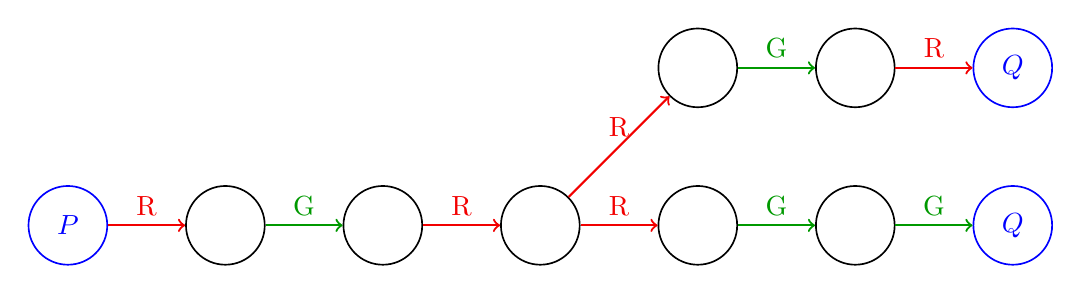
\begin{tikzpicture}[->, semithick]
\tikzset{
    prepost/.style= {circle, draw=blue, color=blue, minimum size=1.0cm},
    pstate/.style= {circle, draw=black, minimum size=1.0cm},
    prel/.style= {above, black!5!red, thick},
    pguar/.style= {above, black!40!green, thick},
}

\node[prepost] (P) at (0,0) {$P$};
\node[pstate] (s1) at (2,0) {};
\node[pstate] (s2) at (4,0) {};
\node[pstate] (s3) at (6,0) {};
\node[pstate] (s4) at (8,0) {};
\node[pstate] (s5) at (10,0) {};
\node[prepost] (s6) at (12,0) {$Q$};

\node[pstate] (s8) at (8,2) {};
\node[pstate] (s9) at (10,2) {};
\node[prepost] (s10) at (12,2) {$Q$};

\draw
(P) edge[prel] node {R} (s1)
(s1) edge[pguar] node {G} (s2)
(s2) edge[prel] node {R} (s3)
(s3) edge[prel] node {R} (s4)
(s4) edge[pguar] node {G} (s5)
(s5) edge[pguar] node {G} (s6)
(s3) edge[prel] node {R} (s8)
(s8) edge[pguar] node {G} (s9)
(s9) edge[prel] node {R} (s10);
\end{tikzpicture}
\captionof{figure}{An interleaving of environment and thread actions abstracted using rely/guarantee relations.}
\end{center}

A predicate $P$ that refers to the structure of a single state, describes a set of possible states, while binary relations represent a set of transitions that can happen in the system \cite{viktor}. The latter are predicates of the form $P_a(\vec{\sigma}, \sigma)$ that relate the state before action $a$ to the one right after. Given a single predicate we can define the two-state relation by placing no constraint on the old state, $P(\sigma) \triangleq P(\vec{\sigma}, \sigma)$ or on the other hand by not restricting the new state $\sigma$, $P(\vec{\sigma}) \triangleq P(\vec{\sigma}, \sigma)$. State relations can be sequentially composed in order to reflect the effect of actual program commands as follows $(P; Q)(\vec{\sigma}, \sigma) \triangleq \exists \alpha \ldotp P(\vec{\sigma}, \alpha) \land Q(\alpha, \sigma)$. We can now define that a binary relation $P$ is stable under another relation $Q$ if and only if $(P; Q) \Rightarrow P \land (Q; P) \Rightarrow P$ which means that whenever an action in $Q$ is done before or after a transition in $P$, this must not invalidate $P$ itself.

Every specification will now take the form $\triplena{R, G}{P}{C}{Q}$ and include the standard pre and postconditions, plus $R$ and $G$, the rely and guarantee relations. The rely relation models all actions that the environment can perform while the guarantee one describes what the thread executing $C$ has the ability to do. In order for the proof to be valid, $G$ needs to be stable under the interference of $R$. Stability is only explicitly checked at the atomic command level \cite{viktor} as the following inference rule describes.

\[
\infer[\textsc{RG-Atomic}]
{
	\triplena{R, G}{P}{\patomic{C}}{Q}
}
{
	\triplena{\mathsf{ID}, \top}{P}{C}{Q}
	\ \
	(P, Q) \in G
	\ \
	\pred{stable}{P, R}
	\ \
	\pred{stable}{Q, R}
}
\]

Given that $C$ executes atomically, there can be no interference from the environment, so $R \equiv \mathsf{ID}$, the identity relation, meaning that the state will be kept as it is. On the other hand, the guarantee relation $G \equiv \top$, allows any operation, although, as part of the premiss, we require the state pair $(P, Q)$ to be part of the original guarantee relation. The hard requirement is the explicit check of stability of $P$ and $Q$ under relation $R$.

\[
\infer[\textsc{RG-Par}]
{
	\triplena{R, G_1 \cup G_2}{P_1 \land P_2}{C_1\ ||\ C_2}{Q_1 \land Q_2}
}
{
	\triplena{R \cup G_2, G_1}{P_1}{C_1}{Q_1}
	\ \
	\triplena{R \cup G_1, G_2}{P_2}{C_2}{Q_2}
}
\]

Commands are composed in parallel using the \textsc{RG-Par} rule that makes the guarantee of the first command be part of the rely relation of the second one and vice-versa. This makes sure that we model all interference coming from concurrent threads.

\newpage

\subsection{Modern Concurrent Reasoning}

\subsection{Hoare Logic}

As a starting point in proving correctness, or generally properties of computer programs, Hoare explains in \cite{hoare} how to use deductive reasoning in applying inference rules to a set of predefined language axioms. He specifies the use of what was later on referred to as a ``Hoare triple" of the shape $\triple{P}{C}{Q}$ where $P$ and $Q$ are first-order assertions while $C$ is the program executed. $P$ is called the precondition of $C$ while $Q$ is its postcondition. The triple thus describes that whenever the assertion $P$ holds before $C$ runs and at some point terminates, then $Q$ will hold on its completion. The kind of logic adopted, allows to reason about relatively simple programs involving integers and local variables living in the \textit{stack} of a function. Classic proofs performed using Hoare logic take the form of a proof tree with axioms as leaves and rules as intermediate steps. Such notation has the downside that complete proofs tend to explode in size. For this reason, proof sketches are utilized. They represent the holding assertions before and after every command that appears in the analyzed code. We can see an example of such in Figure \ref{fig:abshoare}.
\begin{gather*}
\begin{array}{l}
\specline{\top} \\
\pfunctions{abs}{\pvar{x}} \\
	\quad \passign{\pvar{r}}{\pvar{x}}; \\
	\quad \specline{\pvar{x} = \pvar{r}} \\
	\quad \pifelses{\pvar{x} < 0} \\
		\quad \quad \specline{\pvar{x} < 0 \land \pvar{x} = \pvar{r}} \\
		\quad \quad \passign{\pvar{r}}{-\pvar{x}}; \\
		\quad \quad \specline{\pvar{x} < 0 \land \pvar{r} = - \pvar{x}} \\
		\quad \quad \specline{(\pvar{x} < 0 \land \pvar{r} = -\pvar{x}) \lor (\pvar{x} \geq 0 \land \pvar{r} = \pvar{x})} \\
	\quad \pifelsem \\
		\quad \quad \specline{\pvar{x} \geq 0 \land \pvar{x} = \pvar{r}} \\
		\quad \quad \pskip; \\
		\quad \quad \specline{\pvar{x} \geq 0 \land \pvar{x} = \pvar{r}} \\
		\quad \quad \specline{(\pvar{x} < 0 \land \pvar{r} = -\pvar{x}) \lor (\pvar{x} \geq 0 \land \pvar{r} = \pvar{x})} \\
	\quad \pifelsee \\
	\quad \specline{(\pvar{x} < 0 \land \pvar{r} = -\pvar{x}) \lor (\pvar{x} \geq 0 \land \pvar{r} = \pvar{x})} \\
	\quad \preturn{\pvar{r}}; \\
\pfunctione \\
\specline{(\pvar{x} < 0 \land \pvar{ret} = -\pvar{x}) \lor (\pvar{x} \geq 0 \land \pvar{ret} = \pvar{x})} \\
\end{array}
\end{gather*}
\captionof{figure}{A proof sketch of the absolute value function using Hoare logic.}
\label{fig:abshoare} 

The $\mathtt{abs}(\pvar{x})$ function simply returns the absolute value of the input argument $\pvar{x}$. We notice that the procedure's precondition is $\top$ ($true$), which means that there is no particular assertion which needs to hold in order for the code to perform its task. On the other hand, the postcondition states that the return value, which is referred to using a special variable named $\pvar{ret}$, will effectively be the absolute value of $\pvar{x}$. Note how the postcondition of every command in a sequence becomes the precondition of the following one, respecting the rule specified in \cite{hoare}.

\subsection{Owicki-Gries}

In a concurrent setting, the first approach that allowed reasoning of programs was presented in \cite{owicki} and is referred to as the ``Owicki-Gries" method from the name of its authors. Its main contribution is the parallel composition rule.

\[
\infer[\textsc{Owicki-Gries}]
{\vdash \triple{P_1 \land P_2}{C_1\ ||\ C_2}{Q_1 \land Q_2}}
{\vdash \triple{P_1}{C_1}{Q_1} \ \vdash \triple{P_2}{C_2}{Q_2} \ \textsf{interference-free}}
\]

The rule states that we perform a regular sequential proof for each of the threads that are composed together and the resulting postcondition will be the conjunction of all the components' ones. This holds as long as the proofs of the individual thread runs are not interfering with each other. In other words, every intermediate assertion between atomic commands in the sequential proof of $C_1$ must be kept valid by the actions of $C_2$ and vice versa \cite{viktor}.
\[
\infer[\textsc{Cons}]
{
	\triple
	{\pvar{x} = 0}
	{\passign{\pvar{x}}{\pvar{x} + 1}\ ||\ \passign{\pvar{x}}{\pvar{x} + 2}}
	{\pvar{x} = 3}
}
{
	\infer[\textsc{Owicki-Gries}]
	{
		\triple
		{\pvar{x} = 0 \land \pvar{x} = 0}
		{\passign{\pvar{x}}{\pvar{x} + 1}\ ||\ \passign{\pvar{x}}{\pvar{x} + 2}}
		{(\pvar{x} = 1 \lor \pvar{x} = 3) \land (\pvar{x} = 2 \lor \pvar{x} = 3)}
	}
	{
		(\dag)
		\ \ \ \ \ \ \ \ \ \ \ \ \ \ \ \	
		(\spadesuit)
	}
}
\]

\[
(\dag) =
\infer[\textsc{Cons}]
		{
			\triple
			{\pvar{x} = 0}
			{\passign{\pvar{x}}{\pvar{x} + 1}}
			{\pvar{x} = 1 \lor \pvar{x} = 3}
		}
		{
			\infer[\textsc{Assign}]
			{
				\triple
				{\pvar{x} = 0 \lor \pvar{x} = 2}
				{\passign{\pvar{x}}{\pvar{x} + 1}}
				{\pvar{x} = 1 \lor \pvar{x} = 3}
			}
			{\ldots}		
		}
\]

\[
(\spadesuit) = 
\infer[\textsc{Cons}]
		{
			\triple
			{\pvar{x} = 0}
			{\passign{\pvar{x}}{\pvar{x} + 2}}
			{\pvar{x} = 2 \lor \pvar{x} = 3}
		}
		{
			\infer[\textsc{Assign}]
			{
				\triple
				{\pvar{x} = 0 \lor \pvar{x} = 1}
				{\passign{\pvar{x}}{\pvar{x} + 2}}
				{\pvar{x} = 2 \lor \pvar{x} = 3}
			}
			{\ldots}		
		}
\]

\[
\infer[\textsc{Cons}]
	{
		\triple
		{P}
		{C}
		{Q}
	}
	{
		P \Rightarrow P'\ \
		\triple
		{P'}
		{C}
		{Q'}\ \
		Q' \Rightarrow Q
	}
\]
\captionof{figure}{Partial proof tree of a parallel program incrementing variable $\pvar{x}$ which also uses the \textsc{Cons} rule (provided).}

The method's main burden is the \textsf{interference-free} constraint which makes non-trivial commands very complicated to prove. As a consequence, most specifications that satisfy the requirement will be too weak to prove any interesting properties about the concurrent code. This is the reason why such a method is only able to give stronger specifications using auxiliary or ghost variables whose task is to keep track of past program states. In addition, the actual code needs to be augmented with statements that refer to the ghost variables themselves. Any modular use of proofs that involve auxiliary variables would require new specifications, since the number of variables needed to express strong specifications would increase based on the way the module is used (e.g. the number of threads running). This becomes clear by looking at an example of two threads incrementing the same counter concurrently. We first define the counter's methods and then show a summarized proof \cite{modularsteps} of clients' usage through ghost variables.
\begin{gather*}
\begin{array}{@{}l@{\qquad}l@{\qquad}l@{}}
\begin{array}{@{}l@{}}
\pfunctions{makeCounter}{} \\
\quad \palloc{\pvar{c}}{1}; \\
\quad \pmutate{\pvar{c}}{0}; \\
\quad \preturn{\pvar{c}}; \\
\pfunctione
\end{array}
&
\begin{array}{@{}l@{}}
\pfunctions{increment}{\pvar{c}} \\
\quad \texttt{do } \{ \\
	\quad \quad \pderef{\pvar{n}}{\pvar{c}}; \\
	\quad \quad \pfuncall{\pvar{b}}{CAS}{\pvar{c}, \pvar{n}, \pvar{n} + 1}; \\
\quad \} \texttt{ while }(\pvar{b} = 0); \\
\quad \preturn{\pvar{n}}; \\
\pfunctione
\end{array}
\end{array} \\ \\
\pfuncall{\pvar{c}}{makeCounter}{};
\color{ForestGreen}\passign{\pvar{inc}_1}{0};
\passign{\pvar{inc}_2}{0}; \\
\color{blue} \{ \cell{\pvar{c}}{0} \land \pvar{inc}_1 = 0 \land \pvar{inc}_2 = 0 \} \\
\begin{array}{c || c}
\begin{array}{l}
\color{blue} \{ \cell{\pvar{c}}{\pvar{inc}_1 + \pvar{inc}_2} \land \pvar{inc}_1 = 0 \} \\
\texttt{do } \{ \\
	\quad \pderef{\pvar{n}}{\pvar{c}}; \\
	\quad \patomic{\pfuncall{\pvar{b}}{CAS}{\pvar{c}, \pvar{n}, \pvar{n} + 1}; \\
		\quad \quad \textcolor{ForestGreen}{\pifelses{\pvar{b}} \pvar{inc}_1\texttt{++}\pifelsee}} \\
\} \texttt{ while }(\pvar{b} = 0); \\
\color{blue} \{ \cell{\pvar{c}}{\pvar{inc}_1 + \pvar{inc}_2} \land \pvar{inc}_1 = 1 \} \\
\end{array}
&
\begin{array}{l}
\color{blue} \{ \cell{\pvar{c}}{\pvar{inc}_1 + \pvar{inc}_2} \land \pvar{inc}_2 = 0 \} \\
\texttt{do } \{ \\
	\quad \pderef{\pvar{n}'}{\pvar{c}}; \\
	\quad \patomic{\pfuncall{\pvar{b}'}{CAS}{\pvar{c}, \pvar{n}', \pvar{n}' + 1}; \\
		\quad \quad \textcolor{ForestGreen}{\pifelses{\pvar{b}'} \pvar{inc}_2\texttt{++}\pifelsee}} \\
\} \texttt{ while }(\pvar{b}' = 0); \\
\color{blue} \{ \cell{\pvar{c}}{\pvar{inc}_1 + \pvar{inc}_2} \land \pvar{inc}_2 = 1 \} \\
\end{array}
\end{array} \\
\color{blue} \{ \cell{\pvar{c}}{\pvar{inc}_1 + \pvar{inc}_2} \land \pvar{inc}_1 = 1 \land \pvar{inc}_2 = 1 \} \\
\color{blue} \{ \cell{\pvar{c}}{2} \}
\end{gather*}

As we can see, the parts of code in \textcolor{ForestGreen}{green} are auxiliary, i.e. they are not part of the executed code but are there to aid the proof. We use them to build the invariant that each of the two concurrent commands will use to prove its postcondition. In fact, at any point in the concurrent execution, the counter value will be the sum of the two auxiliary variables. Note that the increments to the ghost variables $\mathtt{inc}_1$ and $\mathtt{inc}_2$ must happen atomically with the respective $\mathtt{CAS}$ commands and this is the reason why they are included in an atomic context $\patomic{-}$.

If we now were to prove three separate threads incrementing the same counter in parallel, we would have to redo the proof, adding a new auxiliary variable $\mathtt{inc}_3$ and changing the invariants in all of the other bodies. The solution proposed is therefore not compositional. This implies that whenever we add a new method to a verified module which interacts with some shared state, we need to cross check every new command with all the others already present.

\subsection{Rely/Guarantee}

Jones \cite{jones} introduces a way of explicitly stating the interference coming from the environment as part of concurrent composition of code. This replaces the implicit and tedious side condition in the parallel rule of the ``Owicki-Gries" method. The result is rely/guarantee reasoning which is a compositional method. The specifications that arise from the use of such technique, adopt binary relations to express how the state might change as a result of the running thread's or the environment's actions.

\begin{center}
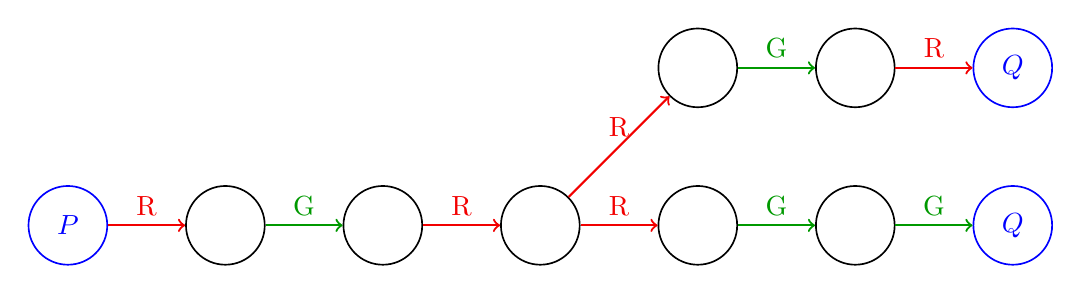
\begin{tikzpicture}[->, semithick]
\tikzset{
    prepost/.style= {circle, draw=blue, color=blue, minimum size=1.0cm},
    pstate/.style= {circle, draw=black, minimum size=1.0cm},
    prel/.style= {above, black!5!red, thick},
    pguar/.style= {above, black!40!green, thick},
}

\node[prepost] (P) at (0,0) {$P$};
\node[pstate] (s1) at (2,0) {};
\node[pstate] (s2) at (4,0) {};
\node[pstate] (s3) at (6,0) {};
\node[pstate] (s4) at (8,0) {};
\node[pstate] (s5) at (10,0) {};
\node[prepost] (s6) at (12,0) {$Q$};

\node[pstate] (s8) at (8,2) {};
\node[pstate] (s9) at (10,2) {};
\node[prepost] (s10) at (12,2) {$Q$};

\draw
(P) edge[prel] node {R} (s1)
(s1) edge[pguar] node {G} (s2)
(s2) edge[prel] node {R} (s3)
(s3) edge[prel] node {R} (s4)
(s4) edge[pguar] node {G} (s5)
(s5) edge[pguar] node {G} (s6)
(s3) edge[prel] node {R} (s8)
(s8) edge[pguar] node {G} (s9)
(s9) edge[prel] node {R} (s10);
\end{tikzpicture}
\captionof{figure}{An interleaving of environment and thread actions abstracted using rely/guarantee relations.}
\end{center}

A predicate $P$ that refers to the structure of a single state, describes a set of possible states, while binary relations represent a set of transitions that can happen in the system \cite{viktor}. The latter are predicates of the form $P_a(\vec{\sigma}, \sigma)$ that relate the state before action $a$ to the one right after. Given a single predicate we can define the two-state relation by placing no constraint on the old state, $P(\sigma) \triangleq P(\vec{\sigma}, \sigma)$ or on the other hand by not restricting the new state $\sigma$, $P(\vec{\sigma}) \triangleq P(\vec{\sigma}, \sigma)$. State relations can be sequentially composed in order to reflect the effect of actual program commands as follows $(P; Q)(\vec{\sigma}, \sigma) \triangleq \exists \alpha \ldotp P(\vec{\sigma}, \alpha) \land Q(\alpha, \sigma)$. We can now define that a binary relation $P$ is stable under another relation $Q$ if and only if $(P; Q) \Rightarrow P \land (Q; P) \Rightarrow P$ which means that whenever an action in $Q$ is done before or after a transition in $P$, this must not invalidate $P$ itself.

Every specification will now take the form $\triplena{R, G}{P}{C}{Q}$ and include the standard pre and postconditions, plus $R$ and $G$, the rely and guarantee relations. The rely relation models all actions that the environment can perform while the guarantee one describes what the thread executing $C$ has the ability to do. In order for the proof to be valid, $G$ needs to be stable under the interference of $R$. Stability is only explicitly checked at the atomic command level \cite{viktor} as the following inference rule describes.

\[
\infer[\textsc{RG-Atomic}]
{
	\triplena{R, G}{P}{\patomic{C}}{Q}
}
{
	\triplena{\mathsf{ID}, \top}{P}{C}{Q}
	\ \
	(P, Q) \in G
	\ \
	\pred{stable}{P, R}
	\ \
	\pred{stable}{Q, R}
}
\]

Given that $C$ executes atomically, there can be no interference from the environment, so $R \equiv \mathsf{ID}$, the identity relation, meaning that the state will be kept as it is. On the other hand, the guarantee relation $G \equiv \top$, allows any operation, although, as part of the premiss, we require the state pair $(P, Q)$ to be part of the original guarantee relation. The hard requirement is the explicit check of stability of $P$ and $Q$ under relation $R$.

\[
\infer[\textsc{RG-Par}]
{
	\triplena{R, G_1 \cup G_2}{P_1 \land P_2}{C_1\ ||\ C_2}{Q_1 \land Q_2}
}
{
	\triplena{R \cup G_2, G_1}{P_1}{C_1}{Q_1}
	\ \
	\triplena{R \cup G_1, G_2}{P_2}{C_2}{Q_2}
}
\]

Commands are composed in parallel using the \textsc{RG-Par} rule that makes the guarantee of the first command be part of the rely relation of the second one and vice-versa. This makes sure that we model all interference coming from concurrent threads.

\subsection{Concurrent Separation Logic}

In order to reason about heap manipulating programs, separation logic was introduced in \cite{seplogic} as a program logic which revolves around the concept of resource owning. The program state does not just involve values local to a method, but also ones that live in the shared \textit{heap} and that variables refer to through pointers. In terms of assertions, the main additions to Hoare's constructs are explained in the following list.
\begin{itemize}
\item The separating conjunction $P \lstar Q$ asserts that the state can be divided into two disjoint parts, one of which satisfies predicate $P$ and the other one $Q$.
\item $\cell{E_1}{E_2}$ asserts that there exists a memory cell whose address can be obtained by evaluating $E_1$ and whose value is $E_2$.
\item The empty assertion $emp$ states that the \textit{heap} must contain no allocated cells.
\end{itemize}

The separating conjunction empowers the program logic to have a frame rule which allows to prove a specification by temporarily not considering additional resources in the heap that are not accessed as part of the command we are verifying.

\[
\infer[\textsc{Frame}]
{\vdash \triple{P \lstar R}{C}{Q \lstar R}}
{\vdash \triple{P}{C}{Q} \ \ \pred{mod}{C} \cap \pred{fv}{R} \equiv \emptyset}
\]

The requirement for it to work, is that no variable which is modified as part of running command $C$ can be free in predicate $R$. Another way of looking at the rule is that if we are able to prove a triple, then adding an arbitrary resource, which is not touched by the command, will not invalidate our original proof. In later work \cite{csl}, O'Hearn included support for disjoint concurrency through a new rule.
\begin{gather*}
\infer[\textsc{SL-Par}]
{\vdash \triple{P_1 \lstar P_2}{C_1\ ||\ C_2}{Q_1 \lstar Q_2}}
{\vdash \triple{P_1}{C_1}{Q_1} \ \vdash \triple{P_2}{C_2}{Q_2} \ \pred{nc}{C_1, C_2, P_2, Q_2} \ \pred{nc}{C_2, C_1, P_1, Q_1}}
\\
\pred{nc}{C, C', P, Q} \triangleq \pred{mod}{C} \cap (\pred{fv}{C'} \cup \pred{fv}{P} \cup \pred{fv}{Q}) \equiv \emptyset
\end{gather*}

The rule states that as long as two threads only access disjoint parts of memory to execute, then they can safely be composed in parallel. The disjointness requirement appears as a side-condition to the rule, expressed through the non conflict predicate $\mathsf{nc}$.

\subsection{RGSep} \label{rgsep}

The efforts developed as part of separation logic and rely/guarantee reasoning were brought together by RGSep \cite{viktor}. Its main contribution was related to the separation between the local state $l$ and shared one $s$. In an abstract sense, $l$ and $s$ are members of a resource algebra $(M, \odot, \mathsf{u})$ such that $l \odot s$ is defined if and only if the two are disjoint. In the latter case, the entirety of the state is defined to be the union of $l$ and $s$. In order to distinguish them, a new kind of assertion, the shared assertion, is introduced and often referred to as the ``boxed assertion". In fact, $\boxed{P}$ expresses a generic separation logic assertion $P$ which refers to the shared state $s$. The separating conjunction $\lstar$ works in the usual way inside of the local state but behaves additively for the shared one. As a consequence we have that $\boxed{P} \lstar \boxed{Q} \Leftrightarrow \boxed{P \land Q}$.

Interference between parallel threads is modelled using actions of the form $P \transto Q$. The action meaning is that the part of the shared state where $P$ holds will be replaced with a part that satisfies $Q$ leaving the rest of $s$ intact. For example, if we were describing the action that allows to increment a counter stored at address $x$, we would have something along the lines of $\cell{x}{n} \transto \cell{x, m} \land m \geq n$.

RGSep requires all preconditions and postconditions of commands in a proof to be stable under interference coming from the environment. We can syntactically check for stability as follows.
\begin{align*}
\pred{stable}{S, \sem{P \transto Q}} &\Leftrightarrow\ \vDash ((P \sepimp S) \lstar Q) \Rightarrow S
\\
\pred{stable}{S, (R_1 \cup R_2)^*} &\Leftrightarrow\ \vDash \pred{stable}{S, R_1} \land \pred{stable}{S, R_2}
\end{align*}
The first property states that if we take a state $S$ and remove the part satisfying $P$ and add one where $Q$ holds then $S$ will hold again. On the other hand, the second property defines that a statement is stable with respect to a set of actions when it is stable under the interference of every action in the set. Given that actions can only affect the shared state $s$, the stability check only needs to be performed on assertions which refer to $s$ itself.

\subsection{CAP}

The program logic explained in \cite{cap} makes use of separation logic constructs to allow abstraction on shared data structures using concurrent abstract predicates. These provide a disjointness of shared resources at the abstraction level which might not be reflected in the actual implementation. For example, if we consider a set module and formulate a predicate stating that ``the set is $\{ 1,2 \}$", then we want to remove element $2$ and be able to assert that the set is now $\{ 1 \}$. In order to reason about the module in such a fine-grained manner, we want element $2$ to be manipulated independently from the rest of the set. This kind of disjointness expressed at the level of abstraction does not need to be part of the implementation. In fact one could implement the set module using a singly linked list which requires traversing some elements before reaching the desired item.

Concurrent abstract predicates also hold information regarding what kind of interference is allowed on the shared memory from the thread and the environment. Fractional permissions \cite{fractional} are utilized in order to model the type of control a thread has on a particular shared structure. On top of this, implementation code can be formally verified against high level specifications and later be \textit{hidden} to clients that make use of it by allowing them not to refer to low-level details in their own proof derivations.

Standard separation logic is augmented with two novel assertions, the shared region and the permission one. The first takes the shape $\sharedr{P}$ and represents a part of memory, associated with an identifier $r$, which is shared among several threads and satisfies predicate $P$. The region is indivisible so that all threads accessing it always get a consistent view of it; we can enforce such behaviour as $\sharedr{P} \lstar \sharedr{Q} \Leftrightarrow \sharedr{P \land Q}$. The permission assertion $[\tguard{A}]_\pi^r$ gives the thread the possibility to perform action $\tguard{A}$ on region $r$ with fractional permission $\pi$. The latter will be a real value in $(0, 1)$ when both the thread and the environment can execute $\tguard{A}$ or equals to $1$ in the case where the thread is the only one to be able to do so. We can combine permissions to perform the same action in the same region in the following way, $[\tguard{A}]_{\pi_1}^r \lstar [\tguard{A}]_{\pi_2}^r \Leftrightarrow [\tguard{A}]_{\pi_1 + \pi_2}^r$. Actions in CAP are similar to the ones seen in Section \ref{rgsep} and have the form $\tguard{A}: P \transto Q$ where the label is followed by two assertions that describe the part of the region needed for $\tguard{A}$ and the same part after the action has taken place. All possible actions for a particular region $r$ are summarized inside $I(r, \vec{x})$. We can create a shared region from a predicate $P \Rrightarrow \exists r \ldotp \sharedr{P} \lstar \pred{all}{I(r, \vec{x})}$ by including every action permission available.

We now have all the ingredients to prove the specification \cite{cap} of a lock module in CAP. The latter will provide three methods, namely \texttt{makeLock()}, \texttt{lock(x)} and \texttt{unlock(x)}. As the names suggest, the first method will allocate the necessary resources for a lock and initiate it while the other two will acquire or release the lock at address $\pvar{x}$. Following these English specifications we can provide formal ones.
\begin{gather*}
\triple
{emp}
{\mathtt{makeLock}()}
{\exists x \ldotp \pvar{ret} = x \land \pred{isLock}{x} \lstar \pred{Locked}{x}}
\\
\triple
{\pred{isLock}{\pvar{x}}}
{\mathtt{lock}(\pvar{x})}
{\pred{isLock}{\pvar{x}} \lstar \pred{Locked}{\pvar{x}}}
\\
\triple
{\pred{Locked}{\pvar{x}}}
{\mathtt{unlock}(\pvar{x})}
{emp}
\end{gather*}

The actions allowed on the lock are $\tguard{L}$ and $\tguard{U}$ which are used to interpret the abstract predicates used in the specification.
\begin{align*}
\pred{isLock}{x} &\equiv \exists r, \pi \ldotp [\tguard{L}]_\pi^r \lstar \sharedrs{(\cell{x}{0} \lstar [\tguard{U}]_1^r) \lor \cell{x}{1}}
\\
\pred{Locked}{x} &\equiv \exists r \ldotp [\tguard{U}]_1^r \lstar \sharedrs{\cell{x}{1}}
\\
I(r, x) &\triangleq 
\left\lbrace
\begin{array}{rl}
\tguard{L}: & [\tguard{U}]_1^r \lstar \cell{x}{0} \transto \cell{x}{1} \\
\tguard{U}: & \cell{x}{1} \transto [\tguard{U}]_1^r \lstar \cell{x}{0}
\end{array}
\right\rbrace
\end{align*}

The $\pred{isLock}{x}$ predicate gives a thread knowledge of the existence of a lock at address $x$ which can either be in the locked or unlocked state based on the value $x$ points to. It also provides a permission to perform the $\tguard{L}$ action to acquire the lock. Given the nature of the predicate we can state that $\pred{isLock}{x} \Rightarrow \pred{isLock}{x} \lstar \pred{isLock}{x}$ holds as we are simply sharing the knowledge of $x$ being a lock.

On the other hand, $\pred{Locked}{x}$ describes that the lock at $x$ is currently locked and has been previously acquired by the thread that holds the predicate. As the $\pred{Locked}{x}$ predicate gives us full permission of $[\tguard{U}]_1^r$, we have that $\pred{Locked}{x} \lstar \pred{Locked}{x} \Rightarrow \bot$ since a thread cannot acquire the lock twice sequentially. Action $\tguard{L}$'s effect requires the lock to be unlocked and for the region to include the permission to perform $\tguard{U}$. In fact, once the action is performed, the latter permission will be removed from the region and included in the thread's local state so that no other thread can release the lock. $\tguard{U}$ has instead the opposite behaviour: it requires the lock to be acquired and once done, it will put the unlock permission back in the shared region. The specification provided will be used to verify a concrete implementation of the lock module using a spin lock whose code is given in Figure \ref{fig:spinlock}.

\begin{figure}
\[
\begin{array}{@{}l@{\qquad}l@{\qquad}l@{}}
\begin{array}{@{}l@{}}
\pfunctions{lock}{\pvar{x}} \\
	\quad \mathtt{do}\ \{ \\
		\quad \quad \pfuncall{\pvar{b}}{CAS}{\pvar{x}, 0, 1}; \\
	\quad \}\ \mathtt{while}\ (\pvar{b} = 0); \\
\pfunctione
\end{array}
&
\begin{array}{@{}l@{}}
\pfunctions{unlock}{\pvar{x}} \\
	\quad \patomic{\pmutate{\pvar{x}}{0}}; \\
\pfunctione
\end{array}
&
\begin{array}{@{}l@{}}
\pfunctions{makeLock}{} \\
	\quad \palloc{\pvar{x}}{1}; \\
	\quad \pmutate{\pvar{x}}{1}; \\
	\quad \preturn{\pvar{x}}; \\
\pfunctione
\end{array}
\end{array}
\]
\captionof{figure}{A spin lock implementation using \texttt{CAS}.}
\label{fig:spinlock}
\end{figure}

The \texttt{lock} method uses a popular mechanism to handle synchronization, namely compare-and-swap. \texttt{CAS}($a$, $c$, $v$) works by atomically comparing the dereferenced value of $a$ with $c$ and in case of a match, $a$ is set to point to $v$. In case of a successful swap, \texttt{CAS} returns 1, otherwise it returns 0.

\begin{figure}
\[
\begin{array}{l}
\specline{\pred{isLock}{\pvar{x}}} \\
\pfunctions{lock}{\pvar{x}} \\
	\quad \specline{\exists r, \pi \ldotp [\tguard{L}]_\pi^r \lstar \sharedrs{(\cell{\pvar{x}}{0} \lstar [\tguard{U}]_1^r) \lor \cell{\pvar{x}}{1}}} \\
	\quad \mathtt{do}\ \{ \\
		\quad \quad \pfuncall{\pvar{b}}{CAS}{\pvar{x}, 0, 1}; \\
		\quad \quad \specline{\exists r, \pi \ldotp \left( [\tguard{L}]_\pi^r \lstar \sharedrs{(\cell{\pvar{x}}{0} \lstar [\tguard{U}]_1^r) \lor \cell{\pvar{x}}{1}} \land \pvar{b} = 0 \right) \\ \lor \left( [\tguard{L}]_\pi^r \lstar [\tguard{U}]_1^r \lstar \sharedr{\cell{\pvar{x}}{1}} \land \pvar{b} = 1 \right)} \\
	\quad \}\ \mathtt{while}\ (\pvar{b} = 0); \\
	\quad \specline{[\tguard{L}]_\pi^r \lstar [\tguard{U}]_1^r \lstar \sharedr{\cell{\pvar{x}}{1}}} \\
\pfunctione \\
\specline{\pred{isLock}{\pvar{x}} \lstar \pred{Locked}{\pvar{x}}}
\end{array}
\]
\captionof{figure}{The spin lock's \texttt{lock} function implementation proof.}
\label{fig:spinproof}
\end{figure}

In Figure \ref{fig:spinproof} we give a CAP sketch proof of the \texttt{lock(x)} method which is shown to satisfy its specification. Note how the use of \texttt{CAS} is combined with a while loop whose condition is the outcome of the swap. This way we can be sure that once the control flow of the program exits the loop, the lock's state is updated and the $\tguard{L}$ action has taken place.

\subsection{Abstract atomicity and Linearizability}

We refer to an operation as atomic when it happens at a single discrete point in time \cite{modularsteps}. Whenever atomic actions are performed concurrently, the actual execution will always be an interleaving of those. In general, even if a command is built from multiple operations, abstract atomicity can be obtained if the overall effect appears to be atomic.

Linearizability \cite{linearizability} is a correctness condition which allows methods of a concurrent module to be used by clients as atomic. All of such module operations are provided with sequential specifications that are proven to behave atomically with respect to each other. As a consequence, the moment a new method is added to the module, the linearizability proof for all methods needs to be performed. The main contribution of the approach is the fact that specifications that guarantee linearizability are an abstraction which can be directly used by clients of the module to reason without having to worry about the implementation details.

\subsection{TaDA} \label{s:tada}

TaDA \cite{tada} is a modern program logic that combines the perks of the CAP approach and of linearizability to allow modular proofs of concurrent programs. Its main novelty is the introduction of atomic specifications as a first-order construct through the use of atomic triples. These have the form $\atriplenl{}{x \in X}{P(x)}{C}{Q(x)}$ and indicate that command $C$ will atomically update the state from $P$ to $Q$ in a single, discrete step.

\begin{center}
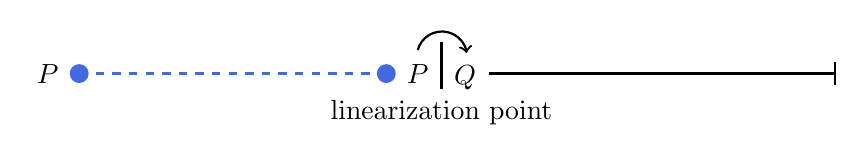
\begin{tikzpicture}[thick]
\node (Ps) at (0, 0) {$P$};
\node (P) at (4.7, 0) {$P$};
\node (Q) at (5.3, -0.05) {$Q$};
\node (L) at (5, -0.5) {linearization point};

\filldraw[color=RoyalBlue] (0.4, 0) circle (3pt);
\filldraw[color=RoyalBlue] (4.3, 0) circle (3pt);
\draw[color=RoyalBlue, dashed] (0.4, 0) -- (4.3, 0);
\draw (5, 0.4) -- (5, -0.2);
\draw (5.6, 0) -- (10, 0);
\draw (10, 0.15) -- (10, -0.15);
\draw [->] (4.7, 0.3) arc (165:8:9pt); 
\end{tikzpicture}
\end{center}

More specifically, the triple actually states that, due to the environment's interference, the variable bound by the pseudo-quantifier $\aall$ (in this case $x$) can vary within the values of set $X$ as long as it still satisfies precondition $P(x)$. Then, right at the function's linearization point, the $C$ command will atomically bring the state to satisfy $Q(x)$. After this, the command does not give any guarantees on the validity of $Q(x)$ since it might be changed by another thread running concurrently. On the other hand, $C$ will not change the state of $x$ again after the linearization point but it can use it to refer to its value right before the event. The specifications give a notion of atomicity which is only maintained at the level of abstraction defined by $P$. In fact, observing the state at a lower level might show several distinct steps involved as part of the command.

We will explore TaDA's rules and constructs while going through a concrete program example of a stack data structure module, which supports concurrent access. The concurrent stack module will have a simple interface for clients to use that allows the creation of a new stack and the ability to push and pop items from it.

Note that the full atomic triple has the shape $\atriplee{}{x \in X}{P_p}{P(x)}{C}{y \in Y}{Q_p(x, y)}{Q(x, y)}$ where the first part of the state is private to the thread. This includes all assertions which are stable under the environment's intereference. Everything which is instead on the public side of the state, accepts interference as described by the guarded transitions for regions. Whenever we encounter a standard Hoare triple $\triple{P}{C}{Q}$ in TaDA, we can see it as pure syntactic sugar for $\atriplenq{}{P}{\top}{C}{Q}{\top}$ where there is effectively no public state.	
\begin{gather*}
\triple{emp}{\mathtt{makeStack}()}{\exists r \ldotp \pred{S}{r, \pvar{ret}, []}}
\\
\atriplenl
{}
{l}
{\pred{S}{r, \pvar{x}, l} \land \pvar{v} \neq 0}
{\pfuncallnr{push}{\pvar{x}, \pvar{v}}}
{\pred{S}{r, \pvar{x}, \pvar{v}\cons l}}
\\
\vatriplenl
{}
{l}
{\pred{S}{r, \pvar{x}, l}}
{\mathtt{pop}(\pvar{x})}
{(\pred{S}{r, \pvar{x}, []} \land \pvar{ret} = 0) \lor (\exists l'\ldotp \pred{S}{r, \pvar{x}, l'} \land l = \pvar{ret}\cons l' \land \pvar{ret} \neq 0)}
\end{gather*}

The \texttt{makeStack()} method is given a sequential specification, since it would be unreal to use a shared structure during its creation. In a more likely setup, a single thread creates the stack and then passes its reference to other (potentially child) threads. The function's return value will be a pointer to the new data structure. Adding elements to the stack is done through the use of \texttt{push}(\texttt{x},\texttt{v}) which puts the item \texttt{v} on top of the stack. We require an atomic specification for the method as the environment might interact with the structure while we are pushing to it. The inserted value must be different from $0$ due to the fact that the return value of \texttt{pop(x)} will be $0$ in the case of an empty stack. This is just a simplified convention, given the abscence of error handling in this demonstrating example. The abstract predicate $\pred{S}{r, x, l}$, in a style similar to CAP, indicates the presence of a stack in the shared region identified by $r$, at memory address $x$ with contents $l$. We can formally define it as follows.
\begin{align*}
\pred{S}{r, x, l} \triangleq &\exists h, ns, ds \ldotp \textbf{Stack}_r(x, h, ns, ds) \lstar [\tguard{G}]_r \land l = \pred{values}{ns}
\\
\text{where } &\pred{values}{[]} \triangleq []
\\
&\pred{values}{(-, v) \cons l} \triangleq v \cons \pred{values}{l}
\end{align*}

The $\textbf{Stack}_r(x, h, ns, ds)$ predicate is a region type describing the structure of a shared region in memory. In addition to that, $[\tguard{G}]_r$ is a guard that is associated to the region as an abstract resource. It gives a thread the permission to perform action $\tguard{G}$ on shared region $r$. Actions in TaDA are defined inside a labelled transition system that maps guards to possible updates to the region. In our case, we express a single guard which gives the ability to both push and pop from the stack. In the second case, the update actually only happens when the stack is non-empty.
\begin{align*}
&\tguard{G}: \forall n, v \neq 0, ns, ds \ldotp (ns, ds) \transto ((n, v) \cons ns, ds)
\\
&\tguard{G}: \forall n, v, ns, ds \ldotp (ns, ds) \transto \ite{ns = (n, v) \cons ns'}{(ns', (n, v) \cons ds)}{(ns, ds)}
\end{align*}

We unveil the meaning of the additional arguments of $\textbf{Stack}_r$ by providing a region interpretation for the latter.
\begin{align*}
I(\textbf{Stack}_r(x, h, ns, ds)) \triangleq &\cell{x}{h} \lstar \mathsf{stack}(h, ns) \lstar \bigoast_{(n, v) \in ds} \twocell{n}{v}{-}
\\
\text{where } &\mathsf{stack}(h, []) \triangleq h = \snull
\\
&\mathsf{stack}(h, (h, v) \cons l) \triangleq v \neq 0 \land \exists z . \twocell{h}{v}{z} \lstar \mathsf{stack}(z, l)
\end{align*}

The stack's address $x$ points to the head node, $h$, which is the first node of the structure that will be either $\snull$ for an empty stack or point to a value and a subsequent node. On top of this, $ns$ is a logical list including all active node pairs $(n, v)$ in the stack where $n$ is the node's address and $v$ the value it points to. Those nodes that were at one point part of the stack but have been popped since, are called dead nodes and included in the set $ds$. As we can see from the transition system, every time an item is popped, it is virtually moved from $ns$ to $ds$ to keep track of it. This additional information, which can be seen as a ghost state of the program, is particularly helpful when proving the \texttt{pop} function implementation. In fact, if the function pops an item $n$ which has been concurrently removed since we first read it, then it is necessary to know that it had the $\twocell{n}{-}{-}$ structure and this information is provided as part of the dead nodes assertion.

\begin{figure}[h]
\[
	\begin{array}{l}
		\pfunction{\pvar{makeStack}}
		{}
		{
		\\
		\quad \palloc{\pvar{x}}{1};
		\\
		\quad \preturn{\pvar{x}}; \\
		}
		\end{array}
		\ \ \ \
		\begin{array}{l}
		\pfunction{\pvar{push}}
		{\pvar{x}, \pvar{v}}
		{
		\\
		\quad \palloc{\pvar{fst}}{2};
		\\
		\quad \pmutate{\pvar{fst}}{\pvar{v}};
		\\
		\\
		\quad \mathtt{do} \ \{
		\\
		\quad \quad \pderef{\pvar{h}}{\pvar{x}};
		\\
		\quad \quad \pmutate{\pvar{fst} + 1}{\pvar{h}};
		\\
		\quad \quad \pfuncall{\pvar{b}}{CAS}{\pvar{x}, \pvar{h}, \pvar{fst}};
		\\
		\quad\} \ \mathtt{while}\ (\pvar{b} = 0);
		\\
		}
		\end{array}
		\ \ \ \
		\begin{array}{l}
		\pfunction{\pvar{pop}}
		{\pvar{x}}
		{
		\\
		\quad \passign{\pvar{r}}{0};
		\\
		\quad \mathtt{do} \ \{
		\\
		\quad \quad \passign{\pvar{b}}{0};
		\\
		\quad \quad \pderef{\pvar{h}}{\pvar{x}};
		\\
		\quad\quad \pifelses{\pvar{h} = \snull}
		\\
		\quad\quad \quad \preturn{0};
		\\
		\quad\quad \pifelsem
		\\
		\quad \quad \quad \pderef{\pvar{r}}{\pvar{h}};
		\\
		\quad \quad \quad \pderef{\pvar{next}}{\pvar{h} + 1};
		\\
		\quad \quad \quad \pfuncall{\pvar{b}}{CAS}{\pvar{x}, \pvar{h}, \pvar{next}};
		\\
		\quad\quad \pifelsee
		\\
		\quad\} \ \mathtt{while}\ (\pvar{b} = 0);
		\\
		\\
		\quad \preturn{\pvar{r}};
		\\
		}
	\end{array}
	\label{fig:concurrentstack}
	\]
	\captionof{figure}{The concurrent stack \textsc{While} language implementation with the addition of the compare-and-swap (\texttt{CAS}) command.}
\end{figure}

We provide an implementation of the three methods in Figure \ref{fig:concurrentstack} followed by a full TaDA proof of the $\pfuncallnr{push}{\pvar{x}, \pvar{v}}$ function. The proof begins by unwrapping the $\pred{S}{r, \pvar{x}, l}$ abstract predicate into its definition which includes the $\textbf{Stack}_r$ region predicate and the $[\tguard{G}]_r$  action guard. We use the latter as part of the \textsc{MakeAtomic} rule, in order to modify the underlying stack structure to insert a new element, $\pvar{v}$. This step gives us the atomicity tracking component $\atomtok$ and the ability of treating a sequence of commands as if they happened atomically. As part of the function's body, we allocate memory for the node (\texttt{fst}) that will host the new element and begin a loop whose task is to read the stack's head node into \texttt{h} and use \texttt{CAS} to atomically set it to \texttt{fst} only when \texttt{h} is equivalent to $[\pvar{x}]$ (meaning that the value of the stack's head has not changed since we first read it into \texttt{h}). We prove all of this using the following inference rules:
\begin{itemize}
\item \textsc{Existential} in order to get rid of the existential quantifiers on logical variables $h, ns, ds$ and to be able to apply the next rules.
\item The \textsc{AWeakening} rule to turn the logical variables $h, ns, ds$ into pseudo-quantified ones (bound by $\aall$) and to prove an atomic triple referring to the update that follows.
\item \textsc{UpdateRegion} consumes the atomicity tracking component to try and update the shared region $\textbf{Stack}_r$ by first opening it up and revealing its interpretation. Later, the update can either succeed or fail, as described by the rule's postcondition that includes a disjunction.
\item We \textsc{Frame} out all assertions only leaving $\cell{\pvar{x}}{h}$ since this is all we need to conclude the proof. In fact, the $\pfuncallnr{CAS}{\pvar{x}, \pvar{h}, \pvar{fst}}$ command does not modify any other variables a part from $\pvar{x}$.
\item The \textsc{CAS} rule finally allows us to condition the actual update on the boolean return value, $\pvar{b}$ which is used inside the following postconditions to understand whether the swap has happened or not.
\end{itemize}

\newgeometry{margin=2cm}
\[
\small{
\begin{array}{l}
	\quantifierline{\aall l \ldotp} \\
	\aspecline{\pred{S}{r, \pvar{x}, l} \land \pvar{v} \neq 0} \\
	\pfunction{\pvar{push}}{\pvar{x}, \pvar{v}}{ \\
		\quad \aspecline{\pred{S}{r, \pvar{x}, l} \land \pvar{v} \neq 0} \\
		\quad \begin{leftvruled}{abstract}
			\aspecline{\exists h, ns, ds \ldotp \textbf{Stack}_r(\pvar{x}, h, ns, ds) \lstar [\tguard{G}]_r \land l = \pred{values}{ns} \land \pvar{v} \neq 0} \\
			\begin{leftvruled}{atomic exists on $ns$, $ds$}
				\quantifierline{\aall ns, ds \ldotp} \\
				\aspecline{\exists h \ldotp \textbf{Stack}_r(\pvar{x}, h, ns, ds) \lstar [\tguard{G}]_r \land l = \pred{values}{ns} \land \pvar{v} \neq 0} \\
				\begin{leftvruled}{make atomic}
					\acontextline{r : (ns, ds) \transto ((-, \pvar{v}) \cons ns, ds) \land \pvar{v} \neq 0 \vdash} \\
					\specline{\exists h, ns, ds \ldotp \textbf{Stack}_r(\pvar{x}, h, ns, ds) \land l = \pred{values}{ns} \lstar r \Mapsto \atomtok \land \pvar{v} \neq 0} \\
					\palloc{\pvar{fst}}{2}; \pmutate{\pvar{fst}}{\pvar{l}}; \\
					\specline{\exists h, ns, ds \ldotp \textbf{Stack}_r(\pvar{x}, h, ns, ds) \land l = \pred{values}{ns} \lstar r \Mapsto \atomtok \lstar \twocell{\pvar{fst}}{\pvar{v}}{\snull} \land \pvar{v} \neq 0} \\
					\mathtt{do} \ \{ \\
						\quad \specline{\exists h, ns, ds, s \ldotp \textbf{Stack}_r(\pvar{x}, h, ns, ds) \land l = \pred{values}{ns} \lstar r \Mapsto \atomtok \lstar \twocell{\pvar{fst}}{\pvar{v}}{s} \land \pvar{v} \neq 0} \\
						\quad \begin{leftvruled}{open region}
							\quantifierline{\aall h, ns, ds \ldotp}
							\aspecline{\cell{\pvar{x}}{h} \lstar \mathsf{stack}(h, ns) \lstar \bigoast_{(n, v) \in ds} \twocell{n}{v}{-}} \\
							\begin{leftvruled}{frame}
								\quantifierline{\aall h \ldotp} \aspecline{\cell{\pvar{x}}{h}} \\
								\pderef{\pvar{h}}{\pvar{x}}; \\
								\aspecline{\cell{\pvar{x}}{h} \land \pvar{h} = h}
							\quad \end{leftvruled} \\
							\aspecline{\cell{\pvar{x}}{h} \lstar \mathsf{stack}(h, ns) \lstar \bigoast_{(n, v) \in ds} \twocell{n}{v}{-} \land \pvar{h} = h} \\
						\end{leftvruled} \\
						\quad \specline{\exists h, ns, ds, s, a \ldotp \textbf{Stack}_r(\pvar{x}, h, ns, ds) \land l = \pred{values}{ns} \lstar r \Mapsto \atomtok \lstar \twocell{\pvar{fst}}{\pvar{v}}{s} \land \pvar{h} = a \land \pvar{v} \neq 0} \\
						\quad \pmutate{\pvar{fst} + 1}{\pvar{h}}; \\
						\quad \specline{\exists h, ns, ds \ldotp \textbf{Stack}_r(\pvar{x}, h, ns, ds) \land l = \pred{values}{ns} \lstar r \Mapsto \atomtok \lstar \twocell{\pvar{fst}}{\pvar{v}}{\pvar{h}} \land \pvar{v} \neq 0} \\
						\quad \begin{leftvruled}{existential on $h, ns, ds$}
							\specline{\textbf{Stack}_r(\pvar{x}, h, ns, ds) \land l = \pred{values}{ns} \lstar r \Mapsto \atomtok \lstar \twocell{\pvar{fst}}{\pvar{v}}{\pvar{h}} \land \pvar{v} \neq 0} \\
							\begin{leftvruled}{weakening on $h$, $ns$, $ds$}
								\quantifierline{\aall h, ns, ds \ldotp} \\
								\aspecline{\textbf{Stack}_r(\pvar{x}, h, ns, ds) \land l = \pred{values}{ns} \lstar r \Mapsto \atomtok \lstar \twocell{\pvar{fst}}{\pvar{v}}{\pvar{h}} \land \pvar{v} \neq 0} \\
								\begin{leftvruled}{update region}
									\aspecline{\cell{\pvar{x}}{h} \lstar \mathsf{stack}(h, ns) \lstar \bigoast_{(n, v) \in ds} \twocell{n}{v}{-} \land l = \pred{values}{ns} \lstar \twocell{\pvar{fst}}{\pvar{v}}{\pvar{h}} \land \pvar{v} \neq 0} \\
									\begin{leftvruled}{frame, CAS}
										\quantifierline{\aall h \ldotp} \\
										\aspecline{\cell{\pvar{x}}{h}} \\
										\pfuncall{\pvar{b}}{CAS}{\pvar{x}, \pvar{h}, \pvar{fst}}; \\
										\aspecline{(\pvar{b} = 0 \land \cell{\pvar{x}}{h} \land \pvar{h} \neq h)
										\lor (\pvar{b} = 1 \land \cell{\pvar{x}}{\pvar{fst}} \land \pvar{h} = h)}
									\end{leftvruled} \\
									\aspecline{(\pvar{b} = 0 \land \pvar{h} \neq h \land \cell{\pvar{x}}{h} \lstar
									\mathsf{stack}(h, ns) \lstar \twocell{\pvar{fst}}{\pvar{v}}{\pvar{h}}) \\
									\lor (\pvar{b} = 1 \land \pvar{h} = h \land \cell{\pvar{x}}{\pvar{fst}} \lstar
									\twocell{\pvar{fst}}{\pvar{v}}{\pvar{h}} \lstar \mathsf{stack}(\pvar{h}, ns)) \\
									\lstar \bigoast_{(n, v) \in ds} \twocell{n}{v}{-} \land l = \pred{values}{ns} \land \pvar{v} \neq 0}
								\end{leftvruled} \\
								\aspecline{l = \pred{values}{ns} \land \pvar{v} \neq 0 \land ((\pvar{b} = 0 \land \textbf{Stack}_r(\pvar{x}, h, ns, ds) \lstar \twocell{\pvar{fst}}{\pvar{v}}{\pvar{h}} \lstar r \Mapsto \atomtok) \\
								\lor (\pvar{b} = 1 \land \textbf{Stack}_r(\pvar{x}, h, (\pvar{fst}, \pvar{v}) \cons ns, ds)) \lstar r \Mapsto ((ns, ds), ((-, \pvar{v}) \cons ns, ds)))}
							\end{leftvruled} \\
							\specline{((\pvar{b} = 0 \land \textbf{Stack}_r(\pvar{x}, h, ns, ds) \lstar \twocell{\pvar{fst}}{\pvar{v}}{\pvar{h}} \lstar r \Mapsto \atomtok) \\ \lor (\pvar{b} = 1 \lstar r \Mapsto ((ns, ds), ((-, \pvar{v}) \cons ns, ds))) \land l = \pred{values}{ns} \land \pvar{v} \neq 0}
						\end{leftvruled} \\
						\quad \specline{\exists h, ns, ds \ldotp ((\pvar{b} = 0 \land
						\textbf{Stack}_r(\pvar{x}, h, ns, ds) \lstar \twocell{\pvar{fst}}{\pvar{v}}{\pvar{h}}
						\lstar r \Mapsto \atomtok) \\
						\lor (\pvar{b} = 1 \lstar r \Mapsto ((ns, ds), ((-, \pvar{v}) \cons ns, ds)))  \land l = \pred{values}{ns} \land \pvar{v} \neq 0} \\
					\} \ \mathtt{while}(\pvar{b} = 0); \\
					\specline{\exists h, ns, ds \ldotp l = \pred{values}{ns} \lstar r \Mapsto ((ns, ds), ((-, \pvar{v}) \cons ns, ds))} \\
				\end{leftvruled} \\
				\aspecline{\exists h \ldotp \textbf{Stack}_r(\pvar{x}, h, (-, \pvar{v}) \cons ns, ds) \lstar [\tguard{G}]_r \land l = \pred{values}{ns}} \\
			\end{leftvruled} \\
			\aspecline{\exists h, ns, ds \ldotp \textbf{Stack}_r(\pvar{x}, h, (-, \pvar{v}) \cons ns, ds) \lstar [\tguard{G}]_r \land l = \pred{values}{ns}} \\
		\end{leftvruled} \\
		\quad \aspecline{\pred{S}{r, \pvar{x}, \pvar{v}\cons l}} \\
	}
\end{array}
}
\]
\restoregeometry

As part of the logic, there are some key inference rules that are displayed in the \texttt{push} proof. For an exhaustive list and explanation we point the reader to \cite{tada}. First of all, \textsc{MakeAtomic} allows to take an atomic specification and prove the abstract atomicity of a sequence of non-atomic commands where a single linearization point will appear and update the shared state. In order to do so, we must hold the guard of the appropriate action for the region. In the premiss, we obtain the atomicity tracker component in the form of an abstract resource ($\atomtok$). This works like a token used to recognize whether the atomic update declared in the atomicity context ($\acontextline{a : x \transto f(x)}$) has already happened or not. On a successful update, the token will be converted into the state transition described by the guarded action. As we can see from the postcondition of the premiss, the atomic update \textit{must} happen at some point in order to satisfy the rule.
\begin{gather*}
f : X \rightarrow Y \ \ \left\lbrace (x, y)\ |\ x \in X, y \in f(x) \right\rbrace \subseteq \mathcal{T}_\textbf{t}^* \\
\infer
{
\atriplenl
	{}
	{x \in X}
	{\textbf{t}_a(\vec{z}, x) \lstar [\tguard{G}]_a}
	{C}
	{\exists y \in f(x) \ldotp \textbf{t}_a(\vec{z}, y) \lstar [\tguard{G}]_a}
}
{
\triplena
	{\acontextline{a : x \in X \transto f(x)}}
	{\exists x \in X \ldotp \textbf{t}_a(\vec{z}, x) \lstar a \Mapsto \atomtok}
	{C}
	{\exists x \in X, y \in f(x) \ldotp a \Mapsto (x, y)}
}
\\
\textsc{MakeAtomic}
\end{gather*}

The moment we need to access the contents of a shared region to unveil its interpretation, we can use one of two rules: \textsc{OpenRegion} and \textsc{UpdateRegion}. The first one allows to view the underlying content of a region but it forbids any update to its abstract state. For this reason, it neither needs an explicit guard nor a tracking component to be used. On the other hand the \textsc{UpdateRegion} rule is employed to perform the atomic update of the region's abstract state. It requires the update not to have happened already and we can guarantee that with the presence of the atomicity token in the precondition. Inside the postcondition we need to take into account whether the update has succeeded or not and we do that by having a disjunction on the two possible predicates that hold for the region.
\begin{gather*}
\infer
{
\atriplenl
{\acontextline{a : x \in X \transto f(x)}}
{x \in X}
{\textbf{t}_a(\vec{z}, x) \lstar P(x) \\
	\lstar a \Mapsto \atomtok}
{C}
{\exists y \in f(x) \ldotp \textbf{t}_a(\vec{z}, y) \\ \lstar Q_1(x, y) \lstar
		a \Mapsto (x, y) \lor \\ \textbf{t}_a(\vec{z}, x) \lstar Q_2(x) \lstar a \Mapsto \atomtok}
}
{
\atriplenl
	{}
	{x \in X}
	{I(\textbf{t}_a(\vec{z}, x)) \lstar P(x)}
	{C}
	{\exists y \in f(x) \ldotp I(\textbf{t}_a(\vec{z}, y)) \lstar Q_1(x, y) \\
		\lor I(\textbf{t}_a(\vec{z}, x)) \lstar Q_2(x)}
}
\\
\textsc{UpdateRegion}
\end{gather*}

Another way to update a shared region is to apply the \textsc{UseAtomic} rule which grants the permission to perform such change through an explicit guard held in the precondition, in contrast with the atomicity tracking component in \textsc{UpdateRegion}. The use of this inference rule implies that command $C$ acts atomically at an abstraction level which is lower than the one of region $a$ and as a consequence, it will be atomic at the higher level as well. This way we can stack a layer of abstraction on top of another which gives a lot of flexibility in terms of writing program modules that extend or make use of other pre-verified modules.
\begin{gather*}
f : X \rightarrow Y \ \ \left\lbrace (x, y)\ |\ x \in X, y \in f(x) \right\rbrace \subseteq \mathcal{T}_\textbf{t}^* \\
\infer
{
\atriplenl
{}
{x \in X}
{\textbf{t}_a(\vec{z}, x) \lstar [\tguard{G}]_a}
{C}
{\exists y \in f(x) \ldotp \textbf{t}_a(\vec{z}, y) \lstar [\tguard{G}]_a}
}
{
\atriplenl
{}
{x \in X}
{I(\textbf{t}_a(\vec{z}, x)) \lstar [\tguard{G}]_a}
{C}
{\exists y \in f(x) \ldotp I(\textbf{t}_a(\vec{z}, y)) \lstar [\tguard{G}]_a}
}
\\
\textsc{UseAtomic}
\end{gather*}

Finally, the \textsc{Frame} rule works in the same way as in separation logic, by adding resources to the precondition and postcondition of a command that does not modify them. As we can notice in the \texttt{push} proof, we can also frame out predicates referring to variables bound by $\aall$.
\begin{gather*}
\pred{mod}{C} \cap \pred{vars}{R_p} \equiv \emptyset\ \
\pred{mod}{C} \cap \pred{vars}{R(x)} \equiv \emptyset \\
\infer
{
	\atriple
	{}
	{x \in X}
	{P_p \lstar R_p}
	{P(x) \lstar R(x)}
	{C}
	{Q_p(x, y) \lstar R_p}
	{Q(x, y) \lstar R(x)}
}
{
	\atriplee
	{}
	{x \in X}
	{P_p}
	{P(x)}
	{C}
	{y \in Y}
	{Q_p(x, y)}
	{Q(x, y)}
}
\\
\textsc{Frame}
\end{gather*}

\newpage

\subsection{Database Theory}

\tocless\subsection{Transactions}

A database is a collection of data items that hold values. A database system (\textit{DBS}) is a tool comprised of software and hardware components that manages access to the underlying database. It allows its users to perform specific operations on the database items. Those can be summarized as being one of two kinds, reads and writes. In the following, we will use the notation \tread{x} to represent a read operation of the database item named \textit{x} while \twrite{x}{v} to depict a write operation which sets item \textit{x}'s value to \textit{v}. We will use the shorthand notation \twritee{x} to mean that some value is written to item $x$. Both the mentioned kind of operations are executed atomically \cite{ccontrol}. This means that the execution of a set of such operations appears to be sequential in terms of its constituents.

It is often the case that several operations are grouped together in order to make them behave as if they were a single unit of work. In such situations, database transactions are used: an ordered collection of operations. For example, considering a database for bank accounts, we consider a transfer of funds as a single operation from the user's point of view even if in reality the \textit{DBS} performs multiple sequential reads and writes to achieve the goal, as shown in Figure \ref{fig:transfer}. A transaction execution must provide guarantees on the well known \textbf{ACID} properties \cite{dbconcepts}, an acronym for:
\begin{enumerate}[ref=(\arabic*)]
\item \label{acid.a} Atomicity: all of the transaction's operations are executed or none of them; there is no possible partial execution of a transaction.
\item \label{acid.c} Consistency: an isolated execution of a transaction maintains the consistency constraints of the database. In our bank example, the property would be maintained when money is neither created nor destroyed as part of a transfer, but simply \textit{moved}.
\item \label{acid.i} Isolation: a transaction executes as if no other one is running in the \textit{DBS} at the same time. More generally, a given isolation level determines the correct behaviours of transactions that run concurrently. For example, serializability implies that any two transactions running in parallel believe that the other one has either finished before they started or it will start after they finished executing.
\item \label{acid.d} Durability: once a transaction has completed its work, all of its changes are kept in the database even if failures happen in the future.
\end{enumerate}

In order to maintain property \ref{acid.a}, a transaction needs to communicate the completion of its operations or its interruption in case of failure. This is done by introducing two new types of operation, namely commit and abort, which are notated \tcommit and \tabort respectively. In the case of an abort, the \textit{DBS} must roll-back the state of the database to what it was prior to the start of the transaction in order to undo the changes performed up to the failure point.

\begin{center}
\begin{tabular}{c@{\hskip 0.5in}c}
\begin{lstlisting}
BEGIN
	balance := R[a]
	W[a, balance-100]
	balance := R[b]
	W[b, balance+100]
	C
END
\end{lstlisting}
&
\begin{lstlisting}
BEGIN
	balance := R[a]
	W[a, balance-5000]
	A
END
\end{lstlisting}
\end{tabular}
\captionof{figure}{Two examples of transactions on the bank database. Note how the second one aborts due to a failure (potentially insufficient funds).}
\label{fig:transfer}
\end{center}

Following the explanation in \cite{ccontrol}, we formally define a transaction $T$ as the tuple $(\theta, \sqsubset)$ where $\theta$ is the set of all operations in $T$ and $\sqsubset$ is a partial order on $\theta$. The latter is defined as:
\[
	\theta \subseteq \left\lbrace op\ |\ op \in \lbrace \tread{x}^i, \twritee{x}^i \rbrace, x \in \pred{items}{db}, i \in \mathds{N} \right\rbrace \cup \left\lbrace \tcommit, \tabort \right\rbrace
\]
The set of operations, $\theta$, maintains the constraint $\left(\tcommit \in \theta \Leftrightarrow \tabort \notin \theta\right)$ while the ordering relation, $\sqsubset$, must satisfy the property that if the transaction contains an operation $t$ which is either a commit or an abort, then all operations must appear in a transaction before $t$. Formally,
\[
	\forall t \in \{\tcommit, \tabort\} \ldotp t \in \theta \Rightarrow \left( \forall op \in \theta \ldotp op \neq t \Rightarrow op \sqsubset t \right)
\]

Also, we state that, as part of a single transaction, any two operations that involve a particular item, with at least one of them being a write, must be ordered according to $\sqsubset$:
\begin{gather*}
	\forall x \in \pred{items}{db}, op, i, j \ldotp \left( op \in \left\lbrace \tread{x}^i, \twritee{x}^i \right\rbrace \land \lbrace op, \twritee{x}^j \rbrace \subseteq \theta \land i \neq j \right) \\ \implies (\twritee{x}^j \sqsubset op \lor op \sqsubset \twritee{x}^j)
\end{gather*}
For the example in Figure \ref{fig:transfer} we would have the following transaction definition:
\begin{gather*}
\theta \equiv \left\lbrace \tmread{\texttt{a}}^1, \tmread{\texttt{b}}^2, \tmwritee{\texttt{a}}^3, \tmwritee{\texttt{b}}^4, \tcommit \right\rbrace
\\[0.4em]
\sqsubset\ \equiv \{ (\tmread{\texttt{a}}^1, \tmwritee{\texttt{a}}^3), (\tmread{\texttt{b}}^2, \tmwritee{\texttt{b}}^4), (\tmread{\texttt{a}}^1, \tcommit), (\tmread{\texttt{b}}^2, \tcommit), (\tmwritee{\texttt{a}}^3, \tcommit), (\tmwritee{\texttt{b}}^4, \tcommit) \}
\end{gather*}
This gives the \textit{DBS} the option to arbitrarily schedule the operations which are not ordered according to $\sqsubset$. In fact, under the mentioned example, one could invert the order of the two reads (or even run them in parallel) and still always get to the same final result. As we will see in section \ref{histories}, if a history is proven to be serializable, then we can guarantee valuable properties about it.

\tocless\subsection{Histories} \label{histories}

Modern database systems employ concurrency in order to run multiple transactions at the same time to achieve a higher performance and better operations throughput. On the downside, running operations in parallel on shared data items can lead to race conditions and a potential loss of two of the aforementioned ACID properties, consistency and isolation.

% In order to investigate the matter further, we will introduce some definitions which will prove useful.
The interleaving of operations which arises from a concurrent run of transactions, is referred to as a history. It records the order in which operations actually happen on the database and given that some of them could effectively execute in parallel, they are not totally ordered. A history $H$ \cite{ccontrol} is therefore a tuple $(\Theta, \pord)$ such that for a set of $n$ transactions $T_H = \left\lbrace T_i \right\rbrace_{i \in I}$, where $I = \{ i\ |\ 1 \leq i \leq n\}$, we have the operations set $\Theta$ and the partial order $\pord$ such that:
\[
	\begin{array}{c}
		\Theta \triangleq \bigcup_{i = 1}^{n} \theta_i\
		\text{ and }\
		\bigcup_{i = 1}^{n} \sqsubset_i\ \subseteq \pord
	\end{array}
\]
When inside a history, single operations are tagged with the transaction they belong to, e.g. $\tread{x}^n_i$ refers to a read with identifier $n$ performed on item $x$ by transaction $i$. Whenever we omit the superscript and the subscript, we assume that they are implicitly existentially quantified.

Let's now define two operations as conflicting if they both access the same data item and one of them is a write; formally we describe the property as:
\begin{gather*}
	\pred{conflict}{op_\alpha, op_\beta} \\
	\iff \\
	op_\alpha \neq op_\beta \land \left(\left( op_\alpha \in \{ \tread{x}, \twritee{x} \} \land op_\beta = \twritee{x} \right) \lor \left( op_\alpha = \twritee{x} \land op_\beta \in \{ \tread{x}, \twritee{x} \} \right)\right)
\end{gather*}
We then require that all conflicting operations appearing in a history must be somehow ordered by $\pord$.
\[
	\forall op_\alpha, op_\beta \ldotp (\pred{conflict}{op_\alpha, op_\beta} \land\left\lbrace op_\alpha, op_\beta \right\rbrace \subseteq \Theta) \Rightarrow (op_\alpha \pord op_\beta \lor op_\beta \pord op_\alpha)
\]
When considering a history $H_{total}$ which is a total order over the operations of its transactions, we can refer to it simply by $\twritee{x}_i^1, $ $\twritee{y}_j^1, $ $\tcommit_i, $ $\tread{x}_j^2, $ $\twritee{x}_j^3, $ $\tcommit_j$ for example.

For every history $H = (\Theta, \pord)$ we can compute the group of transactions which committed as part of it as the set:
\[
	\pred{committed}{H} \triangleq \{ T_i\ |\ \tcommit_i \in \Theta \}
\]
This definition will aid us in describing a fundamental structure for the analysis of histories, the precedence or serialization graph. The latter allows to establish relationships between the transactions committing their operations as part a history. We can now build a history's precedence graph $G(H) = (V, E)$ where the set of vertices $V = \pred{committed}{H}$ includes all committed transactions in $H$ and an edge $(T_i, T_j)$ is in $E$, if transaction $T_i$ has an operation which is ordered before one in $T_j$ and the two are conflicting \cite{dbconcepts}. Formally, the set of edges is defined as:
\[
	E \triangleq \{ (T_i, T_j)\ |\ i \neq j \land \exists op_\alpha, op_\beta \ldotp op_\alpha \in \theta_i \land op_\beta \in \theta_j \land op_\alpha\ \pord\ op_\beta \land \pred{conflict}{op_\alpha, op_\beta} \}
\]

In Figure \ref{fig:exPrecGraph} we can see a concrete instance of a history with $3$ transactions and its corresponding precedence graph. Note that the graph's nodes include the three transactions since they all commit as part of $H$. On top of this, the edge from $T_1$ to $T_2$ is justified by pair the conflicting operations $(\tmread{x}_1^1, \tmwritee{x}_2^2)$, while the one from $T_1$ to $T_2$ by the pair $(\tmread{y}_1^2, \tmwritee{y}_3^1)$.\\

\begin{center}
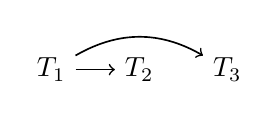
\begin{tikzpicture}[->, semithick]
\node (1) {$T_1$};
\node (2) [right = 0.5cm of 1] {$T_2$};
\node (3) [right = 0.5cm of 2] {$T_3$};

\path
(1) edge node {} (2)
(1) edge [bend left] node {} (3);
\end{tikzpicture}
\\[0.4em]
$H \equiv \tmread{x}_1^1, \tmread{x}_2^1, \tmread{y}_1^2, \tmwritee{x}_2^2, \tcommit_2, \tmwritee{y}_3^1, \tcommit_1, \tcommit_3$
\captionof{figure}{An example history with its corresponding precedence graph.}
\label{fig:exPrecGraph}
\end{center}

A history $H_i$ is said to be equivalent to another history $H_j$ \cite{ccontrol}, when they have the same set of transactions which committed as part of them, and they order conflicting operations in the same way. We formally write $H_i \equiv H_j$, and this holds if and only if:
\begin{gather*}
	\pred{committed}{H_i} \equiv \pred{committed}{H_j} \\
	\land \forall op_\alpha, op_\beta \ldotp (\pred{conflict}{op_\alpha, op_\beta} \land \left\lbrace op_\alpha, op_\beta \right\rbrace \subseteq \Theta_i) \Rightarrow (op_\alpha\ \pord_i\ op_\beta \Leftrightarrow op_\alpha\ \pord_j\ op_\beta)
\end{gather*}
The latter condition is necessary because the result of a concurrent execution of a set of transactions only depends upon the relative ordering of conflicting operations. We describe a history as serial if all of its constituent transactions are run one after the other, without an interleaving of their operations. Such histories guarantee the highest possible database isolation. It is possible to further state that any history $H$ is serializable if and only if it is equivalent to some serial history $H'$. The serializability theorem states that any history $H$, such that its precedence graph $G(H)$ contains no cycles, is serializable \cite{ccontrol}.

\tocless\subsection{Anomalies and Isolation Levels}

The \textsc{Ansi/Iso Sql-92} standard \cite{ansi92} defines a set of different transaction isolation levels based on partial histories they allow as part of the possible interleavings. We will call these sequences of actions phenomena. The original standard describes 3 of such phenomena, while Berenson et al. \cite{isolationansi} add an extra one \ref{ansi:0} for completeness. \\

\begin{enumerate}[label=(\textbf{P\arabic*})]\addtocounter{enumi}{-1}
\item \label{ansi:0} A \textbf{dirty write} appears when a transaction $T_i$ writes to a data item and, before it commits or aborts, another transaction $T_j$ writes to the same item. If any of $T_i$ and $T_j$ were to abort, it is not clear what value the item should contain.
\\
E.g. $H_{DW} \equiv \ldots \tmwritee{x}_i \ldots \tmwritee{x}_j \ldots$
\item We have the \textbf{dirty read} phenomenon in the case where transaction $T_i$ writes to an item, then, before it commits or aborts, another transaction $T_j$ reads that same data item. In fact if $T_i$ would abort after $T_j$ has already read, the latter would have retrieved a value for the item that never actually existed.
\\
E.g. $H_{DR} \equiv \ldots \twritee{x}_i \ldots \tread{x}_j \ldots$
\item A \textbf{non-repeatable read} happens when a transaction $T_i$ reads a data item which is later written to by another transaction $T_j$ that also commits. At this point, if $T_i$ is to read the same item again, it would either discover a new value or fail due to a removal.
\\
E.g. $H_{NR} \equiv \ldots \tread{x}_i \ldots \twritee{x}_j \ldots \tcommit_j \ldots$
\item The \textbf{phantom} phenomenon appears when transaction $T_i$ queries all data items satisfying a particular condition $\gamma$. Transaction $T_j$ then inserts some new items that satisfy $\gamma$. Now, if $T_i$ were to reproduce the initial query, it would see new items appear.
\\
E.g. $H_{P} \equiv \ldots \tmread{\gamma}_i \ldots \tmwritee{\gamma}_j \ldots \tmread{\gamma}_i \ldots$ here we abuse the transaction notation in the following way $\tmread{\gamma} \triangleq \left\lbrace x\ |\ x \in \pred{items}{db} \land \gamma(x) \right\rbrace$ and $\tmwritee{\gamma} \triangleq \exists x, v \ldotp \gamma(x) \land \tmwrite{x}{v}$.
\end{enumerate}

The listed definitions can be used to formulate the \textsc{Ansi} isolation levels as they appear in Table \ref{table:isolation}. The choice of how to concurrently run several transactions given by a $DBS$ allows clients to achieve a better performance or stronger consistency depending on how strict the isolation level is. In fact, allowing some of the phenomena can lead to failing constraint checks in the database.
\begin{center}
\captionof{table}{\textsc{Ansi} isolation levels and the phenomena they allow \cite{ansi92} \cite{isolationansi}.}
\def\arraystretch{1.4}
	\begin{tabular}{l|c c c c}
		\hline
		\textbf{Isolation Level} & \textbf{Dirty Write} & \textbf{Dirty Read} & \textbf{N-R Read} & \textbf{Phantom} \\
		\hline
		Read Uncommitted & $\times$ & \checkmark & \checkmark & \checkmark \\
		Read Committed & $\times$ & $\times$ & \checkmark & \checkmark \\
		Repeatable Read & $\times$ & $\times$ & $\times$ & \checkmark \\
		Serializable & $\times$ & $\times$ & $\times$ & $\times$ \\
		\hline
	\end{tabular}
\label{table:isolation}
\end{center}

A concrete example of how the presence of the described phenomena can lead to a lack of correctness is shown in Table \ref{table:inconsistent} where transactions run at the read committed level. Let's assume that $T_i$ is executed by a bank's agent that wants to read what percentage of the overall funds are held by customer $a$ and $T_j$ is directly performed by $a$ as a cash withdrawal from an ATM machine. The former would first read the balance of $a$ then sum the funds of all customers (in this case $a$, $b$, $c$) and perform a simple division. On the other hand, $T_j$ will first read the cash availability, then subtract $\$100$ and provide the money to the customer. Given the isolation level selected, a non-repeatable read appears as part of history $H$ as $T_j$ removes the money after $T_i$ has read the initial balance for $a$ and before it has computed the overall sum. Therefore the end result $(\texttt{b}\div\texttt{total})$ will be incorrect and larger than the actual one. Moreover, this is a consequence to the fact that $H$ is not serializable. We can show this by first noticing that there are two possible serial histories:
\begin{align*}
	H_1 &= \tmread{a}_1^1, \tmread{a}_1^2, \tmread{b}_1^3, \tmread{c}_1^4, \tcommit_1, \tmread{a}_2^1, \tmwritee{a}_2^2, \tcommit_2 \\[0.5em]
	H_2 &= \tmread{a}_2^1, \tmwritee{a}_2^2, \tcommit_2, \tmread{a}_1^1, \tmread{a}_1^2, \tmread{b}_1^3, \tmread{c}_1^4, \tcommit_1
\end{align*}
The conflicting operations that happen as part of the execution are the pairs $(\tmread{a}_1^1, \tmwritee{a}_2^2)$ and $(\tmread{a}_1^2, \tmwritee{a}_2^2)$. The relative order in which they appear in the histories we consider is expressed as follows:
\[
	\begin{array}{c}
		H: \tmread{a}_1^1\ \pord_H\ \tmwritee{a}_2^2\ \pord_H\ \tmread{a}_1^2
		\\[0.5em]
		\begin{array}{c c}
			H_1 : \tmread{a}_1^1\ \pord_{H_1}\ \tmread{a}_1^2\ \pord_{H_1}\ \tmwritee{a}_2^2\
			&\
			H_2 : \tmwritee{a}_2^2\ \pord_{H_2}\ \tmread{a}_1^1\ \pord_{H_2}\ \tmread{a}_1^2
		\end{array}
	\end{array}
\]
It is clear that the particular ordering of conflicts in $H$ is neither the same as the one in $H_1$, nor to the one in $H_2$. Therefore since $H$ is not equivalent to any of $H_1$ and $H_2$, it is clearly not serializable. A plausible solution for this kind of issue is to change the isolation level of the $DBS$ to repeatable read which forbids the presence of the culprit phenomenon.
\begin{center}
\captionof{table}{History $H$ showing a concurrent run of two transactions $T_i$ and $T_j$.}
\def\arraystretch{1.4}
\begin{tabular}{c|@{\hspace{15pt}} c @{\hspace{15pt}} c}
\hline
\textbf{Time $t$} & $T_i$ & $T_j$ \\
\hline
0 & \texttt{b} = $\tmread{a}_i^1$ & \texttt{c} = $\tmread{a}_j^1$ \\
1 & - & $\tmwrite{a}{\texttt{c}-100}_j^2$ \\
2 & - & \tcommit \\
3 & \texttt{total} = $\tmread{a}_i^2$ + $\tmread{b}_i^3$ + $\tmread{c}_i^4$ & - \\
4 & \tcommit & - \\
\hline
\end{tabular}
\label{table:inconsistent}
\end{center}

\tocless\subsection{Locking Protocols}

The most popular mechanism to enforce a particular isolation level is to use some form of locking. We can consider each data item $x \in \pred{items}{db}$ to be associated with a lock that manages the access to its value. When a transaction runs an operation which accesses $x$, it is required to hold the lock relative to the item. The exact synchronization structure used in this case is a read/write lock that works under two modes, a shared one and an exclusive one. The former allows multiple read operations to happen in parallel while the latter makes sure that there is only one write operation executing at any point in time. This way, execution blocking only happens when transactions perform concurrent conflicting operations on the same data item. In terms of notation, a transaction $T_i$ can lock an item using $\tlock{\kappa}{x}_i$ and unlock it with $\tunlock{\kappa}{x}_i$ where $\kappa \in \{ \tshared, \texclusive \}$ is the lock mode (shared or exclusive). If a transaction requests access to item $x$ and gets an immediate grant even if $x$'s lock is held by another transaction, we say that the two locks are compatible \cite{dbconcepts}. We define this property for lock modes as follows:
\[
	\pred{compatible}{\kappa, \kappa'} \iff (\kappa = \tshared \land \kappa' = \tshared)
\]

We can specify the usage of locks in a formal way by describing histories $H$ that arise from locking protocols. Given that all accesses to database items are well locked, we know that they must be guarded by the corresponding and appropriate locks which are later released, so:
\begin{gather*}
	\forall x, i \ldotp \left( \tmwritee{x}_i \in \Theta_H \implies \tlock{\texclusive}{x}_i\ \pord\ \tmwritee{x}_i\ \pord\ \tunlock{\texclusive}{x}_i \right) \\[0.3em]
	\land \left( \tmread{x}_i \in \Theta_H \implies \exists \kappa \ldotp \tlock{\kappa}{x}_i\ \pord\ \tmread{x}_i\ \pord\ \tunlock{\kappa}{x}_i \right)
\end{gather*}
On top of this, when that a transaction requests an already acquired and non-compatible lock, it must wait for the counterpart to release. This implies that as part of locking protocols' histories, we will see that:
\begin{gather*}
	\forall x, \kappa_a, \kappa_b, i, j \ldotp \\
	(i \neq j \land \lnot \pred{compatible}{\kappa_a, \kappa_b} \land \{ \tlock{\kappa_a}{x}_i, \tunlock{\kappa_a}{x}_i, \tlock{\kappa_b}{x}_j, \tunlock{\kappa_b}{x}_j \}\subseteq \Theta_H) \\
	 \implies (\tunlock{\kappa_b}{x}_j\ \pord\ \tlock{\kappa_a}{x}_i \lor \tunlock{\kappa_a}{x}_i\ \pord\ \tlock{\kappa_b}{x}_j)
\end{gather*}

Two-Phase-Locking (\tpl) is a concurrency control protocol which is vastly used in commercial $DBS$ products. In its base version, as the name suggests, each transaction $T_i$'s execution can be divided into two phases \cite{ccontrol}: a growing phase where $T_i$ sequentially acquires locks for all the data items it is going to access, and a shrinking phase that starts on the first lock release and will unlock all the items it holds, one after the other. According to \tpl, during the growing phase no locks are released, and once the shrinking phase has started, no locks are acquired. Formally, all histories that result from the use of \tpl\ will have an additional property in comparison to the ones already mentioned for locking protocols. In fact lock operations will be further ordered as to comply with the two phase separation:
\[
	\forall x, y, \kappa_a, \kappa_b, i \ldotp (\{ \tlock{\kappa_a}{x}_i, \tunlock{\kappa_b}{y}_i \} \subset \Theta_H \implies \tlock{\kappa_a}{x}_i\ \pord\ \tunlock{\kappa_b}{y}_i)
\]

A variation of the method is Conservative Two-Phase-Locking (\textsc{c2pl}) that works in a similar way with the key difference that all locks ever needed as part of a transaction are acquired before any read or write operation happens. As a consequence, we can state that all histories $H$ adhering to \textsc{c2pl} will be such that:
\[
	\forall x, op, \kappa, i \ldotp (op \neq \textsf{L} \land \{ \tlock{\kappa}{x}_i, op \} \subseteq \Theta_H) \Rightarrow \tlock{\kappa}{x}_i\ \pord\ op
\]
This is done primarily in order to prevent situations in which \tpl\ would exhibit deadlocks, since lock acquisitions can be done in some precise order that all transactions need to follow.

Another version of \tpl\ which is widely used inside concrete implementations is Strict Two-Phase-Locking (\stpl) which imposes a different kind of constraint. Specifically, it only allows transactions to release the locks they hold after they have either committed or aborted. Its histories follow the rules listed for standard \tpl\ and moreover they guarantee that:
\[
	\forall x, op, \kappa, i \ldotp (op \in \{ \tcommit_i, \tabort_i \} \land \{ \tunlock{\kappa}{x}_i, op \} \subset \Theta_H) \Rightarrow op\ \pord\ \tunlock{\kappa}{x}_i
\]
The Strong-Strict Two-Phase-Locking (\textsc{ss2pl}) protocol works by combining the two previous approaches in a way that all locking operations happen before any access to items and all unlocking operations appear after a transaction's commit or abort completion. We summarize the pecularities of the four variants of the protocol in Table \ref{table:2plvariants}. Gradual locking refers to a transaction acquiring locks for cells as it needs to, while the extreme version makes it obtain all needed locks before starting. Similarly, gradual unlocking releases locks whenever they are no longer needed (while still following the two phases rule) and, on the other hand, extreme unlocking only releases locks after a transaction has committed.
\begin{center}
\captionof{table}{Two-Phase-Locking variants' constraints.}
\setlength{\tabcolsep}{14pt}
\def\arraystretch{1.6}
\begin{tabular}{l|c c c c}
\hline
\textbf{Constraint} & \textsc{2pl} & \textsc{c2pl} & \textsc{s2pl} & \textsc{ss2pl} \\
\hline
Gradual Locking & \checkmark & $\times$ & \checkmark & $\times$ \\
Extreme Locking & $\times$ & \checkmark & $\times$ & \checkmark \\
Gradual Unlocking & \checkmark & \checkmark & $\times$ & $\times$ \\
Extreme Unlocking & $\times$ & $\times$ & \checkmark & \checkmark \\
\hline
\end{tabular}
\label{table:2plvariants}
\end{center}

\tocless\subsection{Serializability \& Transactional Models}

\label{sec:serTransMod}

The theory for database transactions that we introduced so far has recently had a large number of applications to the more general context of programming languages. Transactions are being effectively used in the latter to provide an overall simplification to shared-memory concurrency. Popular commercial programming languages provide syntactic constructs to embed a chunk of code into an atomic transaction. This allows to free programmers from the burden of mantaining the fictional atomicity of operations, and delegate everything to the language implementation. We explore two models of transactions in this setting. On top of this, we later explain work related to reasoning about consistency models within distributed databases. \\

\paragraph{Push/Pull Model}
The model of transactions described in \cite{pushPull} is presented as a general theory of serializability, that abstracts away all of the algorithm and implementation details, in order to find a compact set of operations used in the vast majority of cases. The model does not use a concrete machine state, i.e. a global storage or memory heap, to track the effect of transactions' operations such as writes. Instead, it assigns a local \textit{log} of operations to each transaction and considers a unique shared log, which records the history of all globally visible operations. The semantics allow transactions to \textsc{Push} or \textsc{Unpush}, in order to share their local effects with the global log or to recall them from it. Conversely, they can \textsc{Pull} an operation from the shared log into their local view, together with detangling from one through an \textsc{Unpull}. These two types of actions can be seen as reading or \textit{forgetting} a read from the global storage. The framework comes with a proof of serializability within the semantic model, meaning that once users map their algorithms to the \textit{Push/Pull} semantic rules, they obtain a proof of serializability as a consequence.

\paragraph{Semantics for Transactions} The work done in \cite{semanticsTransactions} presents a set of formal languages which are able to describe particular behaviours that arise from the use of transactions within a programming language. Those are defined in terms of small-step operational semantics that allow the interleaving of parallel operations. They are high-level in order not to appear too complicated to the eyes of a programmer, while still detailed enough to express the required features. The languages of the \textsf{AtomsFamily} are listed here, in increasing order of consistency strictness:
\begin{enumerate}
	\item \label{highLevel.1} As part of \textsf{StrongBasic} only one single thread is allowed to execute a transaction at one time. On top of this, a running transaction cannot spawn a new thread and other parallel threads cannot read or write memory cells from the global heap. This is the strongest and simplest of the languages.
	
	\item The \textsf{StrongNestedParallel} language is an extension of the one described in (\ref{highLevel.1}). It allows to spawn threads within transactions in multiple ways. The expression $\mathsf{spawn_{oc}}$, \textit{spawn on commit}, is allowed anywhere in a program, but if included in a transaction, the spawned thread only starts reducing once the parent transaction completes execution. $\mathsf{spawn_{ip}}$, \textit{internally parallel}, is only allowed within a transaction and the latter can only commit once the spawned thread has completed.
	
	\item \label{highLevel.2} \textsf{Weak} is a modified version of the language in (\ref{highLevel.1}) with the removal of the nontransactional code constraint. As a consequence, threads running in parallel to a transaction can access the shared heap through nontransactional commands.
	
	\item Finally, the \textsf{WeakUndo} language has all the features of the one in (\ref{highLevel.2}) together with the possibility for a transaction to abort, undo all of the heap updates and retry.
\end{enumerate}

\paragraph{Consistency Models} Cerone et al. \cite{ceroneConcur15} define a general framework for transactional consistency models within the context of distributed systems, in particular of geo-replicated databases. In this scenario, guaranteeing that the database behaves as if transactions get executed serially is often too slow, or unfeasible due to network failures. This is the main reason why weaker consistency guarantees are taken into account, which allows the occurrence of behaviours prohibited by serializability. The framework itself enables to uniformly specify a variety of such models by taking an axiomatic approach, with the goal of reasoning about databases at a high level of abstraction. What is key in finding common ground among a number of consistency models is the property of atomic visibility. This states that it is guaranteed that all or none of the effects of a transaction are visible to others. Replicated database systems typically enforce this behaviour. The crucial difference is then to understand and analyse when the effects become visible.

As part of the framework, reasoning happens at the level of abstract database executions, which are structures of events with particular relations established on them. Each introduced consistency model is specified through consistency axioms that restrict the possible abstract executions. We will go through the high-level details of two of such models to understand how they are generally developed.

The baseline model is \textbf{Read Atomic}, which is defined through two axioms. The internal consistency axiom, \textsc{Int}, ensures that, as part of the body of a transaction, the value read from a database item $x$ is equivalent to the last value written to $x$ or the last value read from it. On the other hand, the external consistency axiom, \textsc{Ext}, enforces that any time a transaction $T$ reads a value from item $x$ before it writes to it, it will obtain a value which was written to $x$ by transactions preceding $T$. In the case where no transaction wrote to $x$, the default value of $0$ will be returned.

The \textit{precedence} between transactions is given by the visibility relation, \textsf{VIS}. We write $T_1 \xrightarrow{\mathsf{VIS}} T_2$ in order to express that $T_2$'s internal operations can be influenced by $T_1$'s effect on the database. Another fundamental relation of abstract executions is arbitration, \textsf{AR}, which is defined on transactions. The meaning of $T_1 \xrightarrow{\mathsf{AR}} T_2$ is that transaction $T_2$'s version of database items supersedes the one written to by $T_1$.

The adoption of the \textbf{Read Atomic} model leads to a variety of anomalies including the one of causality violation, an example of which is graphically shown in Figure \ref{fig:causVio}. In order to forbid this kind of behaviour we are required to strengthen the consistency model with a new axiom, \textsc{TransVis}. Causal consistency will in fact be obtained by enforcing the \textsf{VIS} relation to be transitive. It follows that the effects of transactions ordered by \textsf{VIS} are observed by others in this same order.
\begin{center}
	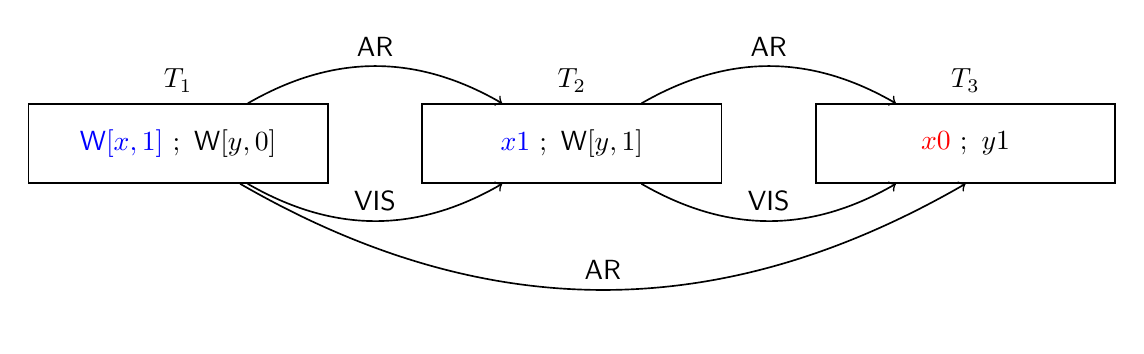
\begin{tikzpicture}[->, semithick]
		\tikzset{
		    trans/.style= {rectangle, draw=black, color=black, minimum width=3.8cm, minimum height=1cm},
		    vis/.style= {above, black!5!black, semithick},
		}
		
		\node[trans] (s1) at (0, 0) {$\textcolor{blue}{\tmwrite{x}{1}}\ ;\ \tmwrite{y}{0}$};
		\node[trans] (s2) at (5, 0) {$\textcolor{blue}{\tmreade{x}{1}}\ ;\ \tmwrite{y}{1}$};
		\node[trans] (s3) at (10, 0) {$\textcolor{red}{\tmreade{x}{0}}\ ;\ \tmreade{y}{1}$};
		\node at (0, 0.8) {$T_1$};
		\node at (5, 0.8) {$T_2$};
		\node at (10, 0.8) {$T_3$};
		
		\draw
		(s1) edge[vis, bend right] node[midway, above] {$\mathsf{VIS}$} (s2)
		(s1) edge[vis, bend left] node[midway, above] {$\mathsf{AR}$} (s2)
		(s1) edge[vis, bend right] node[midway, above] {$\mathsf{AR}$} (s3.270)
		(s2) edge[vis, bend right] node[midway, above] {$\mathsf{VIS}$} (s3)
		(s2) edge[vis, bend left] node[midway, above] {$\mathsf{AR}$} (s3);
	\end{tikzpicture}
	\captionof{figure}{An example of the causality violation anomaly.}
	\label{fig:causVio}
\end{center}


\newpage

\section{mCAP Model and Assertions}

\label{sec:mcapModel}

In the following section we provide the first formalisation of the mCAP logic model (where the \textit{m} stands for \textit{modern}). This work builds upon the CAP program logic, presented in Section \ref{sec:cap} and first introduced in \cite{cap}, and borrows some of the definitions and proof strategies from CoLoSL \cite{colosl}. The main novelties introduced in mCAP, as compared to regular CAP, are concerned with freeing its usage as a logic from some hard constraints. mCAP is in fact parametric with respect to the region capabilities (or \textit{guards}) used, it allows multiple region updates at once through the repartitioning operation, and does not enforce the entirety of a region capability to be held in order to construct the region itself.

\subsection{Separation Algebra}

The concept of a \textit{separation algebra} was introduced in \cite{sepalgebra} to abstract from the standard separation logic model for heaps equipped with an operator to compose them. We introduce such concept here and list some of its core properties.

\defn (Separation algebra). A separation agebra $(\mathcal{M}, \bullet, I)$ \cite{views} is a partial, commutative monoid with multiple units, where $\mathcal{M}$ is a set equipped with a partial operator $\bullet : \mathcal{M} \times \mathcal{M} \rightharpoonup \mathcal{M}$ and a unit set $I \subseteq \mathcal{M}$ satisfying:
\begin{itemize}
\item Commutativity: $m_1 \bullet m_2 = m_2 \bullet m_1$ when either is defined.
\item Associativity: $m_1 \bullet (m_2 \bullet m_3) = (m_1 \bullet m_2) \bullet m_3$ when either is defined.
\item Existence of unit: for all $m \in \mathcal{M}$ there exists $i \in I$ such that $i \bullet m = m$.
\item Minimality of unit: for all $m \in \mathcal{M}$ and $i \in I$, if $i \bullet m$ is defined then $i \bullet m = m$.
\item Cancellativity: for all $m_1, m_2, y, z \in \mathcal{M}$ if $m_1 \bullet y = z$ and $m_2 \bullet y = z$ then $m_1 = m_2$.
\end{itemize}

\defn (Ordering). Given a separation algebra $(\mathcal{M}, \bullet, \mathbf{0})$, the ordering relation $\leq : \mathcal{M} \times \mathcal{M}$ is defined as:
\[
	\leq \triangleq \{ (m_1, m_2)\ |\ \exists m \ldotp m_1 \bullet m = m_2 \}
\]
We write $m_1 \leq m_2$ for $(m_1, m_2) \in \leq$.

\defn (Compatibility). Given a separation algebra $(\mathcal{M}, \bullet, \mathbf{0})$, the compatibility property $\sharp : \mathcal{M} \times \mathcal{M}$ is defined as:
\[
	\sharp \triangleq \{ (m_1, m_2)\ |\ \exists m \ldotp m_1 \bullet m_2 = m \}
\]

\defn (Orthogonal). Given a separation algebra $(\mathcal{M}, \bullet, \mathbf{0})$ and an element $m \in \mathcal{M}$, its orthogonal $(-)^\bot_\mathcal{M} : \mathcal{M} \rightarrow \mathcal{P}(\mathcal{M})$ is the set of all elements in $\mathcal{M}$ which are compatible with it.
\[
	(m)^\bot_\mathcal{M} \triangleq \{m'\ |\ m\ \sharp\ m' \}
\]

\defn (Cross-split property) A separation agebra $(\mathcal{M}, \bullet, I)$ complies with the cross-split property iff:
\begin{gather*}
	\forall a, b, c, d, z \ldotp a \bullet b = z \land c \bullet d = z \implies \\ \exists ac, ad, bc, bd \ldotp ac \bullet ad = a \land ac \bullet bc = c \land bc \bullet bd = b \land ad \bullet bd = d
\end{gather*}

\newpage

\subsection{Worlds} \label{worlds}

A \textit{world} is the structure that represents all of the existing resources and their states, together with a way to describe how these can be modified. We now informally present all of a world's components and properties which are later formalised. A world is in fact a \textit{well-formed} triple $(l, g, \mathcal{J})$, where:
\begin{itemize}
	\item The \textit{logical local state} $l$ represents the resources which are locally owned by a thread and are not externally accessible, i.e. no other thread can see nor update them.
	\item The \textit{shared state} $g$ represents all of the globally shared resources which are divided into regions and accessible to all threads.
	\item The \textit{action model} $\mathcal{J}$ describes how, for every region in the shared state, a thread holding a particular \textit{capability} can update the region. Action models include partial functions, one per region, which associate capabilities to \textit{actions}. An action is a pair $(s, s')$ of logical states where $s$ is the \textit{pre-state}, the state of the region before the action is applied, and $s'$ is the \textit{post-state} which is the state of the region after the action takes place.
\end{itemize}

Worlds can be composed whenever they have the same shared state, action model and a disjoint local logical state. We now proceed to define the latter as tuples whose first component is a machine state, the heap, while the second one is a mapping from regions to capabilities held by the thread for that particular region. Given that mCAP is parametric with respect to the partial commutative monoid representing machine states and capabilities, we allow users of the framework to chose a suitable instantiation to tackle a particular program verification.

\begin{param}
	\label{param:machineStates}
	(Machine states pcm).
	Assume a partial, commutative monoid with multiple units which represents \emph{machine states}, $(\mathbb{M}, \bullet_\mathbb{M}, \mathbf{0}_\mathbb{M})$. Elements of $\mathbb{M}$ are ranged over by $m, m_1, \ldots, m_n$.
\end{param}

\begin{param}
	(Primitive capability pcm).
	Assume a partial, commutative monoid with multiple units which represents \emph{primitive capability resources}, $(\mathbb{K}, \bullet_\mathbb{K}, \mathbf{0}_\mathbb{K})$. Elements of $\mathbb{K}$ are ranged over by $\kappa, \kappa_1, \ldots, \kappa_n$.
\end{param}

Given that the shared state in a mCAP world is organized into regions, we require a way to uniquely characterize each of those. We therefore define distinct region identifiers.
\begin{defn}
	(Region identifiers).
	Assume a set of \emph{region identifiers} $\mathsf{Rid}$, ranged over by $r, r_1, \ldots, r_n$.
\end{defn}

\begin{defn}
	(Capability).
	Given a pcm for primitive capabilities, $(\mathbb{K}, \bullet_\mathbb{K}, \mathbf{0}_\mathbb{K})$, the set of \emph{capabilities}, $\mathsf{RKap}$, is defined as the set of partial functions with a finite domain from region identifiers to primitive capabilities.
	\[
		\mathsf{RKap} \triangleq \mathsf{Rid} \overset{\text{fin}}{\rightharpoonup} \mathbb{K}
	\]
	The $\mathsf{RKap}$ set is ranged over by $\rho, \rho_1, \ldots, \rho_n$. Composition on capabilities, $\circ : \mathsf{RKap} \times \mathsf{RKap} \rightharpoonup \mathsf{RKap}$, is defined as follows:
	\[
		(\rho \circ \rho') (r)
			\triangleq
		\begin{cases}
			\rho(r), & \text{if } r \not\in \pred{dom}{\rho'}
			\\
			\rho'(r), & \text{if } r \not\in \pred{dom}{\rho}
			\\
			\rho(r) \bullet_\mathbb{K} \rho'(r), & \text{otherwise}
		\end{cases}
	\]
	The capabilities pcm is defined as $(\mathsf{RKap}, \circ, \mathbf{0}_{\mathsf{RK}})$, where the capability unit set, $\mathbf{0}_{\mathsf{RK}} : \mathsf{Rid} \overset{\text{fin}}{\rightharpoonup} \mathbb{K}$, is the function with an empty domain. 
\end{defn}
One can see region capabilities as a way to record what capabilities are held for regions present in the world's shared state. Such capabilities can be owned by a thread in its local state or be included inside of a region.

A logical state is therefore a pair $(m, \rho)$ where $m \in \mathbb{M}$ is a machine state and $\rho \in \mathsf{RKap}$ is a region capability, describing what resources are owned and which capabilities are held.
\begin{defn}
	(Logical states).
	Given a pcm for machine states $(\mathbb{M}, \bullet_\mathbb{M}, \mathbf{0}_\mathbb{M})$, and one for capabilities $(\mathbb{K}, \bullet_\mathbb{K}, \mathbf{0}_\mathbb{K})$, the set of \emph{logical states}, $\mathsf{LStates}$, ranged over by $l, l_1, \ldots, l_n$ is defined as:
	\[
		\mathsf{LState} \triangleq \mathbb{M} \times \mathsf{RKap}
	\]
	Composition on logical states, $\circ : \mathsf{LState} \times \mathsf{LState} \rightharpoonup \mathsf{LState}$, is defined as:
	\[
		(m, \rho) \circ (m', \rho') \triangleq (m \bullet_\mathbb{M} m', \rho \circ \rho')
	\]
	The logical states unit set is $\mathbf{0}_\mathsf{L} = \{ (m, \rho)\ |\ m \in \mathbf{0}_\mathbb{M} \land \rho \in \mathbf{0}_\mathsf{RK} \}$ and the pcm of logical states is defined as $(\mathsf{LState}, \circ, \mathbf{0}_\mathsf{L})$.
\end{defn}
Given a logical state $l$ we use $l_\mathsf{M}$ and $l_\mathsf{K}$ to refer to its first and second projections respectively.

\begin{defn}
	(Shared states).
	The set of \emph{shared states} $\mathsf{GState}$, ranged over by $g, g_1, \ldots g_n$, is defined as the set of partial functions with a finite domain, mapping region identifiers to logical states:
	\[
		\mathsf{GState} \triangleq \mathsf{Rid} \overset{\text{fin}}{\rightharpoonup} \mathsf{LState}
	\]
	The \emph{combination function}, $\llfloor - \rrfloor : \mathsf{GState} \rightarrow \mathsf{LState}$ is defined as:
	\[
		\llfloor g \rrfloor \triangleq \prod^{\circ}_{r \in \pred{dom}{g}} g(r)
	\]
	The \textit{cross-composition} function between logical states and shared states, $\oplus : \mathsf{LState} \times \mathsf{GState} \rightharpoonup \mathsf{LState}$, is defined as:
	\[
		l \oplus g \triangleq l \circ \llfloor g \rrfloor
	\]
\end{defn}

\begin{defn}
	(Action models).
	The set of \emph{actions} $\mathsf{Action}$, is defined as the set of tuples of logical states.
	\[
		\mathsf{Action} \triangleq \mathsf{LState} \times \mathsf{LState}
	\]
	Actions are used as part of of action models. The set of \emph{action models}, $\mathsf{AMod}$, ranged over by $\mathcal{J}, \mathcal{J}_1, \ldots, \mathcal{J}_n$, is defined as follows.
	\[
		\mathsf{AMod} \triangleq \mathsf{Rid} \overset{\text{fin}}{\rightharpoonup} \mathbb{K} \overset{\text{fin}}{\rightharpoonup} \mathcal{P}(\mathsf{Action})
	\]
	An action model with an empty domain is simply denoted by $\emptyset$.
\end{defn}
We refer to the first component of an action $(l, l')$ as the \emph{pre-state} while the second one as the \emph{post-state}. 

\begin{defn}
	(Well-formedness).
	A given triple $(l, g, \mathcal{J}) : \mathsf{LState} \times \mathsf{GState} \times \mathsf{AMod}$ is \emph{well-formed}, written $\pred{wf}{(l, g, \mathcal{J})}$ when the cross-composition of the local and shared state is defined, the resulting region capability is contained in the action model and the regions in the shared state are the same as the ones described by the action model.
	\[
		\pred{wf}{(l, g, \mathcal{J})} \iff \exists l' \ldotp l \oplus g = l' \land \pred{dom}{l'_\mathsf{K}} \subseteq \pred{dom}{\mathcal{J}} \land \pred{dom}{g} = \pred{dom}{\mathcal{J}}
	\]
\end{defn}

\begin{defn}
	(World).
	The set of all \emph{worlds}, $\mathsf{World}$, ranged over by $w, w_1, \ldots w_n$, is defined as the set of well-formed triples containing a local state, a global one and an action model.
	\[
		\mathsf{World} \triangleq \{ w \in \mathsf{LState} \times \mathsf{GState} \times \mathsf{AMod}\ |\ \pred{wf}{w} \}
	\]
	Composition on worlds, $\bullet : \mathsf{World} \times \mathsf{World} \rightharpoonup \mathsf{World}$, is defined by composing local states and requiring that shared states and action models be identical.
	\[
		(l, g, \mathcal{J}) \bullet (l', g', \mathcal{J}') \triangleq
		\begin{cases}
			(l \circ l', g, \mathcal{J}), & \text{if } g = g' \text{ and } \mathcal{J} = \mathcal{J}' \\ & \text{and } \pred{wf}{(l \circ l', g, \mathcal{J})}
			\\
			\mathsf{undef} & \text{otherwise}
		\end{cases}
	\]
	The worlds pcm is defined as $(\mathsf{World}, \bullet, \mathbf{0}_\mathsf{W})$, where the worlds unit set is defined as any well-defined world whose local state is part of the logical state unit set, $\mathbf{0}_\mathsf{L}$:
	\[
		\mathbf{0}_\mathsf{W} = \{ (l, g, \mathcal{J})\ |\ (l, g, \mathcal{J}) \in \mathsf{World} \land l \in \mathbf{0}_\mathsf{L} \}
	\]
\end{defn}
Given a world $w$, we write $w_\mathsf{L}, w_\mathsf{S}$ and $w_\mathsf{A}$ for its first, second and third projections.

\newpage

\section{Assertions}

Assertions in mCAP follow the ones in standard CAP with the only difference of being parametric with respect to the machine state assertions and capability assertions that describe elements of the given sets $\mathbb{M}$ and $\mathbb{K}$ respectively. Judgements in mCAP have the shape $\Delta \vdash \triple{P}{\mathds{P}}{Q}$ where $P, Q$ are \textit{assertions}, $\mathds{P}$ is a program and $\Delta$ is an \textit{axiom definition}, all defined in this section.

We assume the presence of an infinite set of logical variables, $x \in \mathsf{LVar}$ and logical environments, $\mathsf{LEnv}$, such that $e \in \mathsf{LEnv} \triangleq \mathsf{LVar} \rightarrow \mathsf{Val}$. Logical environments associate logical variables with their values. Also, since mCAP is an extension of CAP, we provide support for abstract predicates used to express concrete properties. We assume to be given a set of predicate environments, $\mathsf{PEnv}$ that associate each predicate name (coming from the set $\mathsf{PName}$) and its arguments, to a set of worlds that satisfy them. Formally $\delta \in \mathsf{PEnv} \triangleq \mathsf{PName} \times \mathsf{Val}^* \rightarrow \mathcal{P}(\mathsf{World})$.

\begin{param}
	(Machine state assertions).
	Assume a set of \emph{machine state assertions} $\mathsf{MAssn}$, ranged over by $\mathcal{M}, \mathcal{M}_1, \ldots, \mathcal{M}_n$. Given the machine states pcm $(\mathbb{M}, \bullet_\mathbb{M}, \mathbf{0}_\mathbb{M})$, assume an assertion semantics function, that maps machine state assertions to the elements of $\mathbb{M}$ it describes:
	\[
		\tsem{-}_-^\textsc{m} : \mathsf{MAssn} \rightarrow \mathsf{LEnv} \rightarrow \mathcal{P}(\mathbb{M})
	\]
\end{param}

\begin{param}
	(Capability assertions).
	Assume a set of \emph{capability assertions} $\mathsf{KAssn}$ ranged over by $\mathcal{K}, \mathcal{K}_1, \ldots, \mathcal{K}_n$ and an associated semantics function that maps such assertions to elements of the capability separation algebra given as $(\mathbb{K}, \bullet_\mathbb{K}, \mathbf{0}_\mathbb{K})$.
	\[
		\tsem{-}_-^\textsc{k} : \mathsf{KAssn} \rightarrow \mathsf{LEnv} \rightarrow \mathcal{P}(\mathbb{K})
	\]
\end{param}

\begin{defn}
	(Assertion syntax).
	Assertions are elements of the $\mathsf{Assn}$ set defined by the following grammar, where $x \in \mathsf{LVar}, r \in \mathsf{Rid}$ and $\alpha \in \mathsf{PName}$. 
	\begin{align*}
		A &::= \mathtt{false}\ |\ \mathtt{emp}\ |\ \mathcal{M}\ |\ [\mathcal{K}]^r \\
		p, q \in \mathsf{LAssn} &::= A\ |\ \lnot p\ |\ \exists x \ldotp p\ |\ p \lor q\ |\ p \sep q\ |\ p \sepimp q \\
		P, Q \in \mathsf{Assn} &::= p\ |\ P \lor Q\ |\ \exists x \ldotp P\ |\ P \sep Q\ |\ \boxed{P}_I^r\ |\ \alpha(\mathds{E}_1, \ldots, \mathds{E}_n) \\
		I \in \mathsf{IAssn} &::= \emptyset\ |\ \{ \mathcal{K} : \exists \vec{y} \ldotp P \leadsto Q \} \cup I \\
		\Delta \in \mathsf{Ax} &::= \emptyset\ |\ \forall \vec{x} \ldotp P \implies Q\ |\ \forall \vec{x} \ldotp \alpha(\vec{x}) \equiv P\ |\ \Delta_1, \Delta_2
	\end{align*}
\end{defn}

The structure of assertions follows from the separation logic one, with the addition of the given capability assertions $[\mathcal{K}]^r$, shared region (or \textit{boxed}) assertions $\boxed{P}^r_I$ and \textit{interference} assertions $I$. Machine state assertions, $\mathcal{M}$ are interpreted over a world's local logical state, i.e. $\mathcal{M}$ holds true when it is satisfied by $m$, as part of $(m, \rho)$, for a $\rho \in \mathbf{0}_\mathsf{RK}$. In a similar way, a capability assertion $[\mathcal{K}]^r$ is true in a logical state $(m, [r \mapsto \kappa])$ for $m \in\mathbf{0}_\mathbb{M}$, a shared region $r$ and capability $\kappa$ that satisfies $\mathcal{K}$. The assertion $\mathtt{emp}$ is only satisfied by the unit of logical states, formally any $l \in \mathbf{0}_\mathsf{L}$. The separating assertion $P \sep Q$ is true of worlds that can be split in two parts such that the first one satisfies $P$ while the second one $Q$. A predicate assertion holds in all worlds belonging to its semantic interpretation as given by the environment $\delta$. The predicate's arguments are evaluated with respect to the logical environment $e$.

An interference assertion $I$, describes actions that are enabled by a particular capability in the form of pre-condition and post-condition. $I$ is checked against the action model $\mathcal{J}$ to verify that, for the region $r$ it describes, every pre-condition $P$ and post-condition $Q$ are satisfied by $\mathcal{J}$'s actions pre- and post-state. The variables that are existentially bound as part of $I$'s action ($\vec{y}$) are set in the logical environment $e$ to be the same when checking for satisfaction of $P$ and $Q$. This is practically done by building (in Definition \ref{defn:interferenceSem}) a \textit{tiny} action model out of the assertions in $I$ and then checking that it is contained inside of $\mathcal{J}$.

Boxed assertions of the shape $\boxed{P}^r_I$ are true of worlds $(l, g, \mathcal{J})$ where the local state is empty, $l \in \mathbf{0}_\mathsf{L}$, and the logical state associated to $r$ inside of $g$ satisfies $P$. We also need to make sure that the interference assertion $I$, attached to region $r$, is satisfied by $\mathcal{J}(r)$, as described in the previous paragraph.

Finally, a syntactic predicate environment $\Delta$, allows to use assertions in order to build a parametric predicate and store its meaning throughout a proof. In Section \ref{sec:mcapLogic} we will study their semantic interpretation and see how are they used.

\begin{defn}
	\label{defn:interferenceSem}
	(Interference assertion semantics).
	The semantics of \emph{interference assertions}, $\tsem{-}^\textsc{i}_{r, e, \delta, \mathcal{J}} : \mathsf{IAssn} \times \mathsf{Rid} \times \mathsf{LEnv} \times \mathsf{PEnv} \times \mathsf{AMod} \rightarrow \mathsf{Rid} \overset{\text{fin}}{\rightharpoonup} \mathbb{K} \overset{\text{fin}}{\rightharpoonup} \mathcal{P}(\mathsf{Action})$, are defined as:
	\begin{align*}
		\tsem{\emptyset}^\textsc{i}_{r, e, \delta, \mathcal{J}}(r')(\kappa) &\triangleq \emptyset
		\\
		\tsem{\mathcal{K}: \exists \vec{y} \ldotp P \transto Q \cup I}^\textsc{i}_{r, e, \delta, \mathcal{J}}(r')(\kappa) &\triangleq
			\tsem{I}^\textsc{i}_{r, e, \delta, \mathcal{J}}(r')(\kappa)
			\cup 
			\begin{cases}
				\emptyset, & \text{if } r' \neq r
				\\
				(l_p, l_q), & \text{if } \exists g_p, g_q, e', \vec{v} \ldotp
				\kappa \in \tsem{\mathcal{K}}^\textsc{k}_e
				\\
				& \land g_p(r) = l_p \land g_q(r) = l_q
				\\
				& \land \forall \dot{r} \neq r \ldotp g_p(\dot{r}) = g_q(\dot{r})
				\\
				& \land (l_p, g_p, \mathcal{J}), e', \delta \vDash P
				\\
				& \land (l_q, g_q, \mathcal{J}), e', \delta \vDash Q
				\\
				& \land e' = e[\vec{y} \mapsto \vec{v}] 
			\end{cases}
	\end{align*}
\end{defn}
The way we determine semantics for interference assertions requires a precise analysis. We are effectively building a function that, once given an interference assertion $I$, region identifier $r$, logical environment, predicate environment and action model returns a new action model, $\mathcal{J}_I$. The latter only describes all of the actions modelled by $I$ and referring to region $r$. In fact, when we intepret a single action's intereference assertion $\mathcal{K}: \exists \vec{y} \ldotp P \transto Q$, we build a function that, once queried for actions in region $r$ associated to a given capability $\kappa$, will return a tuple of logical states $(l_p, l_q)$. Here, $l_p$ is the local state of the a world built as $(l_p, g_p, \mathcal{J})$ that is used, together with a logical environment $e'$ where all of the $\vec{y}$ in $P$ and $Q$ are bound to values, in order to satisfy assertion $P$. In a similary way, $(l_q, g_q, \mathcal{J})$ is constructed to satisfy $Q$ with the same environment $e'$. The shared state components of these \textit{artificial} worlds are such that they are equivalent for all regions but $r$. On top of this, $g_p(r) = l_p$ and $g_q(r) = l_q$. For interference assertions describing a number of actions, we recursively union the result of a single interpretation with the rest of the actions in $I$.

\begin{defn}
	(Assertion semantics).
	Assertion semantics are given with respect to a world $w \in \mathsf{World}$, a logical environment $e \in \mathsf{LEnv}$ and a predicate environment $\delta \in \mathsf{PEnv}$. They tell us whether a configuration $w, e, \delta$ satisfies a particular assertion.
	\begingroup
	\renewcommand*{\arraystretch}{1.5}
	\[
	\begin{array}{r c l}
		(l, g, \mathcal{J}), e, \delta \vDash p
		&
		\iff
		&
		l, e \vDash_\mathsf{SL} p
	\\
		(l, g, \mathcal{J}), e, delta \vDash \boxed{P}_I^r
		&
		\iff
		&
		l \in \mathbf{0}_\mathsf{L} \text{ and } \exists l' \ldotp (l', g, \mathcal{J}), e, \delta \vDash P
		\\ && \text{and } \exists r' \ldotp r' = e(r) \land g(r') = l' \land \tsem{I}^\textsc{i}_{r', e, \delta, \mathcal{J}} \subseteq \mathcal{J}
	\\
		w, e, \delta \vDash \alpha(\mathds{E}_1, \ldots, \mathds{E}_n)
		&
		\iff
		&
		w \in \delta(\alpha, \tsem{\mathds{E}_1}_e^\textsc{e}, \ldots, \tsem{\mathds{E}_n}_e^\textsc{e})
	\\
		w, e, \delta \vDash \exists x \ldotp P
		&
		\iff
		&
		\exists v \ldotp w, e[x \mapsto v], \delta \vDash P
	\\
		w, e, \delta \vDash P \lor Q
		&
		\iff
		&
		w, e, \delta \vDash P \text{ or } w, e, \delta \vDash Q
	\\
		w, e, \delta \vDash P \sep Q
		&
		\iff
		&
		\exists w_1, w_2 \ldotp w = w_1 \bullet w_2 \text{ and } \\ && w_1, e \vDash P \text{ and } w_2, e \vDash Q
	\\
		l, e \vDash_\mathsf{SL} \mathtt{false}
		&&
		\text{never}
	\\
		l, e \vDash_\mathsf{SL}  \mathtt{emp}
		&
		\iff
		&
		l \in \mathbf{0}_\mathsf{L}
	\\
		l, e \vDash_\mathsf{SL} \mathcal{M}
		&
		\iff
		&
		\exists m, \rho \ldotp l = (m, \rho) \text{ and } m \in \tsem{\mathcal{M}}_e^\textsc{m} \text{ and } \rho \in \mathbf{0}_\mathsf{RK}
	\\
		l, e \vDash_\mathsf{SL} [\mathcal{K}]^r
		&
		\iff
		&
		\exists m, \kappa \ldotp l = (m, [r \mapsto \kappa]) \text{ and } \kappa \in \tsem{\mathcal{K}}_e^\textsc{k} \text{ and } m \in \mathbf{0}_\mathbb{M}
	\\
		l, e \vDash_\mathsf{SL} \lnot p
		&
		\iff
		&
		l, e \not\vDash_\mathsf{SL} p
	\\
		l, e \vDash_\mathsf{SL} p \sepimp q
		&
		\iff
		&
		\forall l' \ldotp l', e \vDash_\mathsf{SL} p \text{ implies } l \circ l', e \vDash_\mathsf{SL} q
	\\
		l, e \vDash_\mathsf{SL} p \sep q
		&
		\iff
		&
		\exists l_1, l_2 \ldotp l = l_1 \circ l_2 \text{ and } \\
		&& l_1, e \vDash_\mathsf{SL} p \text{ and } l_2, e \vDash_\mathsf{SL} q
	\\
		 l, e \vDash_\mathsf{SL} p \lor q
		 &
		 \iff
		 &
		 l, e \vDash_\mathsf{SL} p \text{ or } l, e \vDash_\mathsf{SL} q
	\\
		l, e \vDash_\mathsf{SL} \exists x \ldotp p
		&
		\iff
		&
		\exists v \ldotp l, e[x \mapsto v] \vDash_\mathsf{SL} p
	\end{array}
	\]
	\endgroup
\end{defn}
Now, given a logical environment $e \in \mathsf{LEnv}$ and a predicate environment $\delta \in \mathsf{PEnv}$, we write $\tsem{P}_{e, \delta}$ for the set of all worlds satisfying assertion $P$ under the environments $e$ and $\delta$.
\[
	\tsem{P}_{e, \delta} \triangleq \{ w\ |\ w, e, \delta \vDash P \}
\]

Similarly to CAP, the separating conjunction of shared state assertions on the same region is interpreted as a regular non-separating conjunction, $\land$, formally:
\[
	\boxed{P}^r_I \sep \boxed{Q}^r_I \iff \boxed{P \land Q}^r_I
\]
We also syntactically allow nested regions, but they can always be separated. Their semantic meaning is therefore expressed as follows:
\[
	\boxed{\boxed{P}^r_I \sep Q}^{r'}_{I'} \iff \boxed{P}^r_I \sep \boxed{Q}^{r'}_{I'}
\]

\newpage

\section{mCAP Program Logic}

This section is dedicated to the description of a program logic for transactions using the concepts that have already been introduced in **MCAP SECTION**. We start by formally defining what the rely and guarantee relations are for each thread. This allows us to describe the effects of a thread and of the environment on the current world. Such relations allow us to further state \textit{stability} for assertions and for predicate environments, a fundamental property to later on build our proofs. All of these components are then used to formalise the concept of \textit{repartitioning} \cite{cap}\cite{colosl} that logically represents a thread's atomic actions included in its guarantee relation.

\subsection{Environment Semantics}

The rely relation models how the environment, i.e. other running threads, can reorganize or modify a world. All these behaviours are depicted as \textit{interference} from the environment and they can be divided into two kinds: region construction and region update. Before we move on, it is important to state what it means for a region identifier to be fresh inside of a world, as such definition will be used throughout the section.

\begin{defn}
	(Region freshness).
	A region identifier $r$ is \emph{fresh} with respect to a world $w = (l, g, \mathcal{J})$, when $r$ does not appear as part of $w$'s shared state, $g$.
	\[
		\pred{fresh}{r, (l, g, \mathcal{J})}
			\iff
		r \not\in \pred{dom}{g}
	\]
\end{defn}

We model how the environment can create a new region out of existing resources in its own logical local state through the construction rely relation between worlds.
\begin{defn}
	(Construction rely).
	The \emph{construction rely} relation, $R^c : \mathsf{Worlds} \times \mathsf{World}$, is defined as:
	\[
		R^c \triangleq \big\{ (w, w')\ |\ 
			\exists r, l, a \ldotp \pred{fresh}{r, w} \land w'_\mathsf{L} = w_\mathsf{L} \land w'_\mathsf{S} = w_\mathsf{S}[r \mapsto l] \land w'_\mathsf{A} = w_\mathsf{A}[r \mapsto a]
		\big\}
	\]
\end{defn}
The created region must have a fresh identifier $r$, used to map the new shared resources inside of the global state and the allowed actions in the action model. The updated world's local state $w'_\mathsf{L}$, as seen by a thread, will obviously be unmodified given that the environment cannot touch it. The fact that $R^c$ is defined over worlds, which are well-defined by definition, ensures that $w'_\mathsf{L} \circ w'_\mathsf{S}$ is always defined. On top of this, it will also be the case that the local state will not contain any capability for the region that has just been constructed.

The environment can also update an already existing region inside the global state, as long as it holds a capability that entitles it to perform the change.
\begin{defn}
	(Update rely).
	The \emph{update rely} relation, $R^u : \mathsf{Worlds} \times \mathsf{World}$, is defined as:
	\[
		R^u \triangleq \big\{ \left( (l, g, \mathcal{J}), (l, g', \mathcal{J}) \right)\ |\ \exists r, \kappa \ldotp  \kappa\ \sharp\ (l \oplus g)_\mathsf{K}(r) \land (g, g') \in \lceil \mathcal{J}(r) \rceil (\kappa) \big\}
	\]
\end{defn}
An update done by the environment is only allowed to modify the world's shared state $g$, while the local state $l$ and action model $\mathcal{J}$ stay the same. The actual region update is only allowed when the environment makes use of a capability $\kappa$ that is compatible with the capabilities that are currently in the local and shared states. Moreover, $\kappa$ needs to enable the shared state transition as described by $\mathcal{J}(r)$. Since we allow actions to only describe a part of the region they are modifying, and not the entirety of it, we introduce and use the \emph{action framing} function, $\lceil - \rceil : \left( \mathbb{K} \rightarrow \mathcal{P}(\mathsf{Action}) \right) \times \mathbb{K} \rightarrow \mathcal{P}(\mathsf{Action})$.
	\[
		\lceil a \rceil (\kappa) \triangleq \{ (p \circ f, q \circ f)\ |\ (p, q) \in a(\kappa) \land f \in \mathsf{LState} \}
	\]
This way, all of the region resources that are not affected by the update, i.e. $f$, will stay the same in the resulting world.

We now have all of the ingredients to define the overall rely relation between worlds, which describes any behaviour of the environment on the global state and action model.
\begin{defn}
	(Rely relation).
	The \emph{rely} relation, $R : \mathsf{World} \times \mathsf{World}$, is defined as follows.
	\[
		R \triangleq (R^c \cup R^u)^*
	\]
\end{defn}
The transitive closure allows the environment to perform multiple updates and region constructions in one single atomic step, as seen by a thread. This definition is different from CAP's original one \cite{cap}, since the latter only allowed one single update and multiple constructions.

\begin{defn}
	(Stability).
	An assertion $P$ is said to be stable with respect to a predicate environment $\delta \in \mathsf{PEnv}$, written $\mathsf{stable}_\delta(P)$, if and only if, for all $e \in \mathsf{LEnv}$ and $w, w' \in \mathsf{World}$, if $w, e, \delta \vDash P$ and $(w, w') \in R$, then $w', e, \delta \vDash P$.
\end{defn}	
Intuitively, we require the stability property as we need to be sure that any given assertion $P$ which is currently satisfiable, is not going to be invalidated by a rely step done by the environment and modelled through $R$.

\begin{defn}
	(Predicate environment stability).
	A predicate environment $\delta$ is said to be stable, written $\pred{pstable}{\delta}$, if and only if, for all $W \in \pred{range}{\delta}$, for all $w, w' \in \mathsf{World}$, if $w \in W$ and $(w, w') \in R$, then $w' \in W$. The semantics of a syntactic predicate environment $\Delta \in \mathsf{Ax}$ are defined as a set of stable predicate environments that satisfy them:
	\begin{align*}
		\tsem{\emptyset}^\textsc{p} &\triangleq \{ \delta\ |\ \pred{pstable}{\delta} \} \\
		\tsem{\forall \vec{x} \ldotp P \implies Q}^\textsc{p} &\triangleq \{ \delta\ |\ \pred{pstable}{\delta} \land \forall \vec{v} \ldotp \tsem{P}_{\emptyset[\vec{x} \mapsto \vec{v}], \delta} \subseteq \tsem{Q}_{\emptyset[\vec{x} \mapsto \vec{v}], \delta} \} \\
		\tsem{\forall \vec{x} \ldotp \alpha(\vec{x}) \equiv P}^\textsc{p} &\triangleq \{ \delta\ |\ \pred{pstable}{\delta} \land \forall \vec{v} \ldotp \delta(\alpha, \vec{v}) = \tsem{P}_{\emptyset[\vec{x} \mapsto \vec{v}], \delta} \} \\
		\tsem{\Delta_1, \Delta_2}^\textsc{p} &\triangleq \tsem{\Delta_1}^\textsc{p} \cap \tsem{\Delta_2}^\textsc{p}
	\end{align*}
\end{defn}

The effect of a particular thread's actions is modelled through the guarantee relation. A thread can create a new region using currently owned resources in its local state and such behaviour is formally described through the $G^c$ between worlds. On the other hand, we leave region destruction as implicit, i.e. the user can encode it as a special action in the action model associated to the region, which gets rid of everything inside of it.
\begin{defn}
	(Construction guarantee).
	The \emph{construction guarantee} relation, $G^c : \mathsf{World} \times \mathsf{World}$, is defined as:
	\[
	\begin{array}{r | l}
		G^c \triangleq \Bigg\{ (w, w')
		&
		\begin{array}{c}
			\exists r, m, l, l', a, \rho \ldotp \pred{fresh}{r, w} \land \pred{dom}{\rho} = \{r\} \land
			\\
			w_\mathsf{L} = l \circ l' \land w'_\mathsf{L} = l \circ (m, \rho) \land m \in \mathbf{0}_\mathbb{M} \land
			\\
			w'_\mathsf{S} = w_\mathsf{S}[r \mapsto l'] \land w'_\mathsf{A} = w_\mathsf{A}[r \mapsto a]
		\end{array}
		\Bigg\}
	\end{array}
	\]
\end{defn}
As we can see from the definition, a thread is allowed to create a region as long as its identifier $r$ is entirely fresh and the new shared state includes a part of its local state that is moved out of it. In exchange, $w'_\mathsf{L}$ will include capabilities for the new region. The action model is accordingly updated to describe all of the actions allowed on $r$.

We instead model how a thread can modify an existing region in the shared state for which it holds the appropriate capabilities, through the guarantee update relation between worlds. As part of the relation definition, we will make use of the orthogonal of the machine state and capability pcm which is generally defined in the following definition.

\begin{defn}
	\label{defn:orthogonal}
	(Orthogonal).
	Given a pcm $(\mathcal{M}, \bullet, \mathbf{0})$ and an element $m \in \mathcal{M}$, its \emph{orthogonal} $(-)^\bot_\mathcal{M} : \mathcal{M} \rightarrow \mathcal{P}(\mathcal{M})$ is the set of all elements in $\mathcal{M}$ which are compatible with it.
\[
	(m)^\bot_\mathcal{M} \triangleq \{m'\ |\ m\ \sharp\ m' \}
\]
\end{defn}

\begin{defn}
	(Update guarantee).
	The \emph{update guarantee} relation, $G^u : \mathsf{World} \times \mathsf{World}$, is defined as:
	\[
	\begin{array}{r | l}
		G^u \triangleq \Bigg\{ ((l, g, \mathcal{J}), (l', g', \mathcal{J}))
		&
		\begin{array}{c}
			((l \oplus g)_\mathsf{K})_\mathbb{K}^\bot = ((l' \oplus g')_\mathsf{K})_\mathbb{K}^\bot \land \\
			(g = g' \lor \exists r, \kappa \leq l_\mathsf{K}(r) \ldotp (g, g') \in \lceil \mathcal{J}(r) \rceil(\kappa)  \\ \land ((l \oplus g)_\mathsf{M})_\mathbb{M}^\bot = ((l' \oplus g')_\mathsf{M})_\mathbb{M}^\bot )
		\end{array}
		\Bigg\}
	\end{array}
	\]
\end{defn}
A guarantee update enables a thread to change $l$ and $g$ (while not introducing new regions), leaving the action model $\mathcal{J}$ unmodified. During the update, a thread cannot introduce new capabilities as part of its local state or the global shared one. This requirement is enforced by checking that the orthogonal (Definition \ref{defn:orthogonal}) of all capabilities stays the same as part of the transition from $l, g$ to $l', g'$. The update can further leave the global state unmodified (thus only performing a local change) or it is entitled to modify it through an action, as long as the running thread holds an appropriate capability in its local state. As part of an update, there can be a transfer of resources from the local to the shared state together with their mutation. Since we do not want to enable \textit{fictitious} resource creation, we require the guarantee relation to preserve the orthogonal of the local and global machine state's composition as well.

We can finally define the overall guarantee relation between worlds, expressed through $G$.
\begin{defn}
	(Guarantee).
	The \emph{guarantee} relation, $G : \mathsf{World} \times \mathsf{World}$, is defined as:
	\[
		G \triangleq (G^c \cup G^u)^*
	\]
\end{defn}
Similar to the rely relation, the definition uses a transitive closure to allow multiple region creations and updates as part of a single atomic step performed by a thread. This gives the main reason behind the \textit{orthogonal} constraint as part of the update guarantee definition. A practical explanation of why this condition is required is illustrated in the following example. Assume a situation where we instantiate machine states as standard variable stores and we leave capabilities as abstract or not explicitly specified (through the use of $-$). Let's consider what happens when the action model $\mathcal{J}$ has the following action mapping for shared region $r$ and the orthogonal preservation is not required.
\[
	\mathcal{J}(r)
		=
	\left\{
		\begin{array}{r r}
			\kappa_1: & ([x \mapsto 1], \kappa_2) \transto ([x \mapsto 2, y \mapsto 1], \emptyset) \\
			\kappa_2: & ([x \mapsto 2, y \mapsto 1], \emptyset) \transto ([x \mapsto 3], \kappa_2)
		\end{array}
	\right\}
\]
A thread holding capability $\kappa_1$ can use it when $r$ contains $x \mapsto 1$ to update it to $x \mapsto 2$ and introduce out of nowhere, a new resource $y \mapsto 1$, which was not previously held in the thread's local logical state. Moreover, if the obtained capability $\kappa_2$ is used by the same thread as part of the same atomic update to bring the state of the region $r$ directly from $x \mapsto 1$ to $x \mapsto 3$ without one noticing the introduction of the \textit{fictitious} resource $y$. We therefore have the strong constraint on the orthogonal preservation in order to cope with these kind of scenarios.

At this point, we are enabled to explain the fundamental notion of repartitioning with respect to an update from $p$ to $q$, written $P \Rrightarrow^{\{p\}\{q\}} Q$ \cite{cap}. The latter indicates that any world $w_1$ satisfying the assertion $P$ has a machine-state component $(w_1)_\mathsf{M}$ that includes a part, $m_1$, which satisfies the separation logic assertion $p$. Moreover, when $m_1$ is replaced by $m_2$ that satisfies assertion $q$, we are able to reconstruct a world $w_2$ that satisfies $Q$ and for which the transition from $w_1$ to $w_2$ is allowed by the guarantee relation $G$.

\begin{defn}
	(Repartitioning).
	\label{repartitioning}
	The \emph{repartioning} of worlds, written $P \Rrightarrow^{\{p\}\{q\}} Q$, holds if and only if, for every logical environment $e \in \mathsf{LEnv}$, predicate environment $\delta \in \mathsf{PEnv}$, and world $w_1 = (l_1, g_1, \mathcal{J}_1) \in \mathsf{World}$ such that $w_1, e, \delta \vDash P$, there exist states $m_1, m' \in \mathbb{M}$, such that for a $\rho_1 \in \mathbf{0}_\mathsf{RK}$:
	\begin{itemize}
		\item $(m_1, \rho_1), e \vDash_\mathsf{SL} p$ and
		\item $m_1 \bullet_\mathbb{M} m' = (l_1 \oplus g_1)_\mathsf{M}$ and
		\item for every $m_2 \in \mathbb{M}$ and $\rho_2 \in  \mathbf{0}_\mathsf{RK}$ where $(m_2, \rho_2), e \vDash_\mathsf{SL} q$, there exists a world $w_2 = (l_2, g_2, \mathcal{J}_2) \in \mathsf{World}$ such that $w_2, e, \delta \vDash Q$ and
			\begin{itemize}
				\item $m_2 \bullet_\mathbb{M} m' = (l_2 \oplus g_2)_\mathsf{M}$
				\item $(w_1, w_2) \in G$
			\end{itemize}
	\end{itemize}
\end{defn}

We write $P \Rrightarrow Q$ in order to express $P \Rrightarrow^{\{\mathtt{emp}\}\{\mathtt{emp}\}}Q$. The latter allows the shared state to be reorganized around but not to be effectively mutated.


\newpage

\subsection{Programming Language}

\newpage

\subsection{Proof System}

\newpage

\subsection{Operational Semantics}

The operational semantics of the programming language are defined in terms of concrete program states. Given the fact that we are defining an instantiation of the views framework, the operational semantics described here follow the structure defined in \cite{views} provided with the set of concrete states and the interpretation of transactions (i.e. atomic commands).

\begin{param}
	(Concrete states).
	Assume a set of concrete states $\mathcal{S}$ ranged over by $\sigma, \sigma_1, \ldots, \sigma_n$.
\end{param}

\begin{param}
	\label{param:ecmdInt}
	(Elementary command interpretation).
	Given the set of concrete states $\mathcal{S}$, assume an \emph{elementary command interpretation} function associating elementary commands to a state-transformer function:
	\[
		\tsem{\hat{\mathds{C}}}_{\hat{\mathsf{C}}} : \mathsf{ECmd} \rightarrow \mathcal{S} \rightarrow \mathcal{P}(\mathcal{S})
	\]
	The interpretation function is also lifted to a set of concrete states, such that for $S \in \mathcal{P}(\mathcal{S})$:
	\[
		\tsem{\hat{\mathds{C}}}_{\hat{\mathsf{C}}}(S) \triangleq \bigcup_{\sigma \in S} \tsem{\hat{\mathds{C}}}_{\hat{\mathsf{C}}}(\sigma)
	\]
\end{param}

\begin{defn}
	(Commands interpretation).
	The interpretation function for elementary commands, formally $\tsem{-}^s_{\mathsf{C}} : \mathsf{Cmd} \rightarrow \mathcal{S} \rightarrow \mathcal{P}(\mathcal{S})$, is defined as:
	\begin{align*}
		\tsem{\hat{\mathds{C}}}_{\mathsf{C}}(\sigma) &\triangleq \tsem{\hat{\mathds{C}}}_{\hat{\mathsf{C}}}(\sigma)
		\\
		\tsem{\pskip}_{\mathsf{C}}(\sigma) &\triangleq \{ \sigma \}
		\\
		\tsem{\mathds{C}_1 ; \mathds{C}_2}_{\mathsf{C}}(\sigma) &\triangleq \{ \sigma'\ |\ S = \tsem{\mathds{C}_1}_\mathsf{C}(\sigma) \land \sigma' \in \tsem{\mathds{C}_2}_\mathsf{C}(S) \}
		\\
		\tsem{\pif{\mathds{B}}{\mathds{C}_1}{\mathds{C}_2}}_\mathsf{C}(\sigma) &\triangleq \mathbf{if}\ \tsem{\mathds{B}}^\textsc{b}_\sigma\ \mathbf{then}\ \tsem{\mathds{C}_1}_\mathsf{C}(\sigma)\ \mathbf{else}\ \tsem{\mathds{C}_2}_\mathsf{C}(\sigma)
		\\
		\tsem{\ploop{\mathds{B}}{\mathds{C}}}_\mathsf{C}(\sigma) &\triangleq \tsem{\pif{\mathds{B}}{\left(\mathds{C};\ploop{\mathds{B}}{\mathds{C}}\right)}{\pskip}}_\mathsf{C}(\sigma)
	\end{align*}
	where we assume a function for the semantics of boolean expression, $\tsem{-}^\textsc{b}_\sigma : \mathsf{BExpr} \rightarrow \mathcal{S} \rightarrow \mathsf{Bool}$.
	
	The interpretation function is lifted to a set of concrete state such that for $S \in \mathcal{P}(\mathcal{S})$:
	\[
		\tsem{\mathds{C}}_\mathsf{C}(S) \triangleq \bigcup_{\sigma \in S} \tsem{\mathds{C}}_\mathsf{C}(\sigma)
	\]	
\end{defn}
In the case of an elementary command, we simply use Definition \ref{param:ecmdInt} while the interpretation of $\pskip$ is the identity function on the input state $\sigma$. The effect of a sequential composition of two commands is defined as the set of all states arising from the execution of the first command, followed by the second command applied to the resulting states. Loops are rewritten as conditionals, where the if body contains the loop body composed with the same loop. If statements are instead applied to a state by branching on the boolean condition, semantically evaluated under $\sigma$.

\defn (Transactions interpretation). Finally, we can provide the interpretation function for transactions, which is formally defined as $\tsem{-}_\mathsf{T} : \mathsf{Atom} \rightarrow \mathcal{S} \rightarrow \mathcal{P}(\mathcal{S})$,
\[
	\tsem{\ptdef{\mathds{C}}_\iota}_\mathsf{T}(h) \triangleq \{ h'\ |\ \exists s' \ldotp (h', s') = \tsem{\mathds{C}}_\mathsf{C}(h, \emptyset) \}
\]
Therefore, the semantic meaning of running an atomic transaction on the concrete state $h$, is any resulting state $h'$ that results from executing the transaction's body $\mathds{C}$, starting with the same state $h$ and an empty local stack.

We also lift the interpretation function to a set of concrete state such that for $H \in \mathcal{P}(\mathcal{S})$:
\[
	\tsem{\mathds{T}}_\mathsf{T}(H) \triangleq \bigcup_{h \in H}  \tsem{\mathds{T}}_\mathsf{T}(h)
\]	

\newpage

\subsection{Soundness}

\label{sec:mcapSound}

The soundness of mCAP is established by relating its proof judgements to the operational semantics. The link is created through a \textit{reification} function that transforms worlds, as defined in Section \ref{worlds}, to concrete machine states. As we constructed mCAP as an instantiation of the views framework \cite{views}, its soundness follows from the soundness of views, given that the transactions (atomic commands) are shown to be sound with respect to their operational semantics.

\begin{param}
	(Machine state reification).
	Given the partial commutative monoid for machine states $(\mathbb{M}, \bullet_\mathbb{M}, \mathbf{0}_\mathbb{M})$, assume a \emph{reification function} $\lfloor - \rfloor_\mathbb{M} : \mathbb{M} \rightarrow \mathcal{P}(\mathcal{S})$ which associates machine states to sets of concrete ones.
\end{param}

The views framework guarantees soundness of an instantiated logic once we are able to prove its \textit{Axiom Soundness} property, specifically \textbf{Property L} in \cite{views}. This is formulated and proven in Theorem \ref{thm:soundTrans}. Given the structure of the operational semantics for transactions, the proof relies on two other results, namely the axiom soundness of sequential commands and elementary commands. The latter is provided to the framework as a further parameter since elementary commands are themselves parametric.

\begin{param}
	\label{param:ecmdSound}
	(Elementary command soundness).
	Given the pcm for machine states $(\mathbb{M}, \bullet_\mathbb{M}, \mathbf{0}_\mathbb{M})$ and its associated reification function $\lfloor - \rfloor_\mathbb{M}$, assume that for every elementary command $\hat{\mathds{C}} \in \mathsf{ECmd}$, the corresponding axiom $(M_1, \hat{\mathds{C}}, M_2) \in \textsc{Ax}_{\hat{\mathsf{C}}}$ and any given machine state $m \in \mathbb{M}$ the following \emph{soundness} property holds:
	\[
		\tsem{\hat{\mathds{C}}}(\lfloor M_1 \bullet_\mathbb{M} \{m\} \rfloor_\mathbb{M}) \subseteq \lfloor M_2 \bullet_\mathbb{M} \{m\} \rfloor_\mathbb{M}
	\]
\end{param}
Intuitively, the property establishes that, for any given axiom of elementary commands $(M_1, \hat{\mathds{C}}, M_2)$, the operational semantics of $\hat{\mathds{C}}$ are able to transform elements of the reificated machine states set $M_1$ into ones that belong to the reification of $M_2$. Moreover, the property also enforces frame preservation. In fact, it suggests that if we apply the command to the composition of the elements in $\lfloor M_1 \rfloor_\mathbb{M}$ with an arbitrary machine state $m$, then the result will be a subset the reification of elements in $\lfloor M_2 \rfloor_\mathbb{M}$, composed with the same $m$.

\begin{defn}
	(Reification).
	The \emph{reification of worlds}, $\lfloor - \rfloor_W : \mathsf{World} \rightarrow \mathcal{P}(\mathcal{S})$, is defined as follows.
	\[
		\lfloor (l, g, \mathcal{J}) \rfloor_W \triangleq \lfloor (l \circ g)_\mathsf{M} \rfloor_\mathbb{M}
	\]
\end{defn}
We transform worlds into machine states by dropping the action model, composing the local and the shared state together, and removing all of the region capabilities from it in order to only end up with the machine component of the resulting logical state.

\begin{defn}
	(Judgements).
	The syntactic triple $\Delta \vdash \triple{P}{\mathds{P}}{Q}$ is defined in terms of the semantic triple as stated in Views \cite{views} and it holds if and only if
	\[
		\forall e, \delta \ldotp \delta \in \tsem{\Delta}^\textsc{p} \implies \vDash \triple{\tsem{P}_{e, \delta}}{\mathds{P}}{\tsem{Q}_{e, \delta}}
	\]
\end{defn}

In a comparable way to elementary commands, the soundness of transactions is proven by considering an arbitrary transactions' axiom $(W_1, \mathds{T}, W_2)$, built according to Definition \ref{defn:transAx}, together with a world $w$. It is required to show that the operational semantics of $\mathds{T}$, when applied to elements of the reification of $W_1 \bullet_\mathbb{M} \{w\}$, output a concrete state which is a subset of $\lfloor W_1 \bullet_\mathbb{M} R(\{w\}) \rfloor_\mathbb{M}$. Not only we require the semantics to work correctly in terms of what the axioms impose, but also to preserve frames even under the effects of the rely relation. The property in fact ensures that whatever additional world component, $w$, which is not needed by $\mathds{T}$, i.e. its corresponding axiom does not describe it, will remain unchanged upto its rely relation evolutions.
\begin{thm}
	\label{thm:soundTrans}
	(Transaction soundness).
	For all $\mathds{T} \in \mathsf{Trans}, (W_1, \mathds{T}, W_2) \in \textsc{Ax}_\mathsf{T}$ and $w \in \mathsf{World}$:
	\[
		\tsem{\mathds{T}}_\mathsf{T}(\lfloor W_1 \bullet_\mathbb{M} \{ w \} \rfloor_W) \subseteq \lfloor W_2 \bullet_\mathbb{M} R(\{ w \}) \rfloor_W
	\]
	
	{\parindent0pt
	\begin{proof}
	By induction on the structure of $\mathds{T}$. \\	
	
	\textit{Case}: $\ptdef{\mathds{C}}$
	
	Let's pick an arbitrary $\mathds{C} \in \mathsf{Cmd}, w \in \mathsf{World}$ and $W_1, W_2 \in \mathcal{P}(\mathsf{World})$ such that the following holds:
	\[
		(W_1, \ptdef{\mathds{C}}_\iota, W_2) \in \textsc{Ax}_\mathsf{T}
	\]
	From the definition of $\textsc{Ax}_\mathsf{T}$ we know that there exists $M_1, M_2 \in \mathcal{P}(\mathbb{M})$ such that:
	\begin{gather}\label{tsound:1}
		(M_1, \mathds{C}, M_2) \in \textsc{Ax}_\mathsf{C} \land W_1 \Rrightarrow^{\{M_1\}\{M_2\}} W_2
	\end{gather}
	
	\textit{To show}:
	\[
		\tsem{\ptdef{\mathds{C}}}_\mathsf{T}(\lfloor W_1 \bullet \{w\} \rfloor_W) \subseteq \lfloor W_2 \bullet R(\{w\}) \rfloor_W
	\]
	
	Let's pick an arbitrary $w_1 = (l_1, g_1, \mathcal{J}_1) \in W_1$. We are now left to show that there exists a $w_2 \in \mathsf{World}$ and $w' \in R(w)$ such that:
	\[
		\tsem{\ptdef{\mathds{C}}}_\mathsf{T}(\lfloor w_1 \bullet w \rfloor_W) = \lfloor w_2 \bullet w' \rfloor_W
	\]
	
	From the definition of $\tsem{-}_\mathsf{T}, \lfloor - \rfloor_W$, and the properties of $\bullet$ and $\bullet_\mathbb{M}$ we have:
	\begin{align}
		\tsem{\ptdef{\mathds{C}}}_\mathsf{T}(\lfloor w_1 \bullet w \rfloor_W) =\
			&\tsem{\mathds{C}}_\mathsf{C}(\lfloor w_1 \bullet w \rfloor_W) \\
			\label{tsound:2} =\ &\tsem{\mathds{C}}_\mathsf{C}\left( \lfloor (l_1 \oplus g_1)_\mathsf{M} \bullet_\mathbb{M} (w_\mathsf{L})_\mathsf{M} \rfloor_\mathbb{M} \right)
	\end{align}
	
	From (\ref{tsound:1}) and the definition of $\Rrightarrow$ we know there exists $m_1 \in M_1$ and $m' \in \mathbb{M}$ such that:
	\begin{gather}
	\label{tsound:3} m_1 \bullet_\mathbb{M} m' = (l_1 \oplus g_1)_\mathsf{M} \land \\
	\label{tsound:4} \forall m_2 \in M_2 \ldotp \exists w_2 = (l_2, g_2, \mathcal{J}_2) \in W_2 \ldotp m_2 \bullet_\mathbb{M} m' = (l_2 \oplus g_2)_\mathsf{M} \land (w_1, w_2) \in G
	\end{gather}
	
	From (\ref{tsound:2}) and (\ref{tsound:3}) we get:
	\begin{gather}\label{tsound:5}
	\tsem{\ptdef{\mathds{C}}}_\mathsf{T}(\lfloor w_1 \bullet w \rfloor_W) =
	\tsem{\mathds{C}}_\mathsf{C}(\lfloor m_1 \bullet_\mathbb{M} m' \bullet_\mathbb{M} (w_\mathsf{L})_\mathsf{M} \rfloor_\mathbb{M})
	\end{gather}
	
	From (\ref{tsound:1}) and the soundness of commands shown in Theorem \ref{thm:cSound}, we can rewrite (\ref{tsound:5}) as:
	\[
		\tsem{\ptdef{\mathds{C}}}_\mathsf{T}(\lfloor w_1 \bullet w \rfloor_W)
		\subseteq
		\lfloor M_2 \bullet_\mathbb{M} \{m' \bullet_\mathbb{M} (w_\mathsf{L})_\mathsf{M}\} \rfloor_\mathbb{M}
	\]
	
	Which means that there exists a $m_2 \in M_2$ such that:
	\begin{gather}\label{tsound:6}
		\tsem{\ptdef{\mathds{C}}}_\mathsf{T}(\lfloor w_1 \bullet w \rfloor_W)
		=
		\lfloor m_2 \bullet_\mathbb{M} m' \bullet_\mathbb{M} (w_\mathsf{L})_\mathsf{M} \rfloor_\mathbb{M}
	\end{gather}
	
	From (\ref{tsound:4}) we know that there exists $w_2 \in \mathsf{World}$ such that:
	\begin{gather}
	\label{tsound:8} w_2 = (l_2, g_2, \mathcal{J}_2) \in W_2 \land m_2 \bullet_\mathbb{M} m' = (l_2 \oplus g_2)_\mathsf{M} \\
	\label{tsound:7} \land\ (w_1, w_2) \in G
	\end{gather}
	
	From the definition of $\lfloor - \rfloor_W$ and the properties of $\bullet_\mathbb{M}$ and $\bullet$ we can rewrite (\ref{tsound:6}) as:
	\begin{gather}\label{tsound:9}
		\tsem{\ptdef{\mathds{C}}}_\mathsf{T}(\lfloor w_1 \bullet w \rfloor_W)
		=
		\lfloor (l_2 \circ w_\mathsf{L}, g_2, \mathcal{J}_2) \rfloor_W
	\end{gather}
	
	From (\ref{tsound:7}) and Lemma \ref{lem:R} we know that there exists a $w' \in \mathsf{World}$ such that:
	\begin{gather}\label{tsound:10}
		w' = (w_\mathsf{L}, g_2, \mathcal{J}_2) \land w' \in R(w)
	\end{gather}
	
	From (\ref{tsound:8}), (\ref{tsound:9}) and (\ref{tsound:10}) we know that there exists a $w_2 \in W_2$ and $w' \in R(w)$ such that:
	\[
		\tsem{\ptdef{\mathds{C}}}_\mathsf{T}(\lfloor w_1 \bullet w \rfloor_W) = \lfloor w_2 \bullet R(w) \rfloor_W
	\]
	\end{proof}
	}
\end{thm}

\begin{thm}
	\label{thm:mcapSound}
	(Soundness).
	For all predicate axioms $\Delta \in \mathsf{Ax}$, assertions $P, Q \in \mathsf{Assn}$ and program $\mathds{P} \in \mathsf{Prog}$, if $\Delta \vdash \triple{P}{\mathds{P}}{Q}$ then $\Delta \vDash \triple{P}{\mathds{P}}{Q}$.
\end{thm}

\newpage

%\section{Two-Phase-Locking}

\subsection{Model}

\label{sec:2plMod}

In order to formally describe the behaviours that arise from adopting \tpl\ as a concurrency control protocol, we extend the model presented in Section \ref{sec:transLogicMod} by adding two new global constructs and a way to keep track of the locking phase each transaction is currently in. These changes are necessary since we need to enable a real interleaving of concurrent executions and to introduce the concept of locking storage items.

In fact, under the \textsc{2pl} protocol, all accesses to the shared storage cells must be protected by a corresponding lock. This means that any transaction that needs to read or write a particular cell must be granted an appropriate lock for that same cell. The abstract locks we use, behave in a standard way: depending on the mode, they can have zero, one or more \textit{owners}, i.e. threads that have been granted access to the protected cells.

\begin{defn}
	(Lock modes).
	The set of \emph{lock modes}, $\mathsf{Lock}$, is ranged over by $\kappa, \kappa_1, \ldots, \kappa_n$ and defined as:
	\[
		\mathsf{Lock} \triangleq \{ \textsc{u}, \textsc{s}, \textsc{x} \}
	\]
	The associated strict total order, $>$, is defined in the following way:
	\[
		>\ \triangleq \{ (\textsc{x}, \textsc{u}), (\textsc{x}, \textsc{s}), (\textsc{s}, \textsc{u}) \}
	\]
	The total order $\geq$ on the set $\mathsf{Lock}$ is equivalent to $>$ unioned with all of the reflexive pairs.
\end{defn}
We informally refer to each of the lock mode entries as \textit{unlocked}, \textit{shared} and \textit{exclusive} respectively. This reflects the fact that either no transaction is accessing a cell, one or more transactions are allowed to read the cell's content or a single transaction has been given the permission to write to the cell.

The \textsc{2pl} protocol sets a precise constraint on the pattern of acquisition and release of locks. A transaction $\mathds{T}$'s lifecycle is clearly distinguished between two phases. It initially starts executing in the \textit{growing} phase ($\curlywedge$), where it is free to sequentially acquire locks  for any cell it needs. Once it releases one of the locks it is holding, the transaction enters the \textit{shrinking} phase ($\curlyvee$). Here $\mathds{T}$ is denied any new lock acquisitions while it is allowed to gradually release the locks that are still being held.
\begin{defn}
	(Locking phase).
	 The set of \emph{locking phases}, ranged over by $p$, is defined as:
	 \[
	 	\mathsf{Phase} \triangleq \{ \curlywedge, \curlyvee \}
	 \]
\end{defn}
We sometimes refer to the growing and shirinking phase using \textit{acquiring} and \textit{releasing} phase respectively.

At this point we have all of the ingredients to introduce the other main component of our model, the lock manager. This global structure records the status of all locks on storage cells.

\begin{defn}
	(Lock manager).
	A \emph{lock manager} is defined as a total function with a finite domain from storage keys to pairs of transaction identifiers and lock modes.
	\[
		\mathsf{LMan} \triangleq \mathsf{Key} \xrightarrow{\text{fin}} \mathcal{P}(\mathsf{Tid}) \times \mathsf{Lock}
	\]
	The $\mathsf{LMan}$ set is ranged over by $\Phi, \Phi_1, \ldots, \Phi_n$. In order to cope with the default state of locks associated to keys initially absent from the domain of a lock manager, a total function, $\hat{-}(-) : \mathsf{LMan} \times \mathsf{Key} \rightarrow \mathcal{P}(\mathsf{Tid}) \times \mathsf{Lock}$, is defined as:
	\[
		\hat{\Phi}(k)
			\triangleq
		\begin{cases}
			\Phi(k), & \text{if } k \in \pred{dom}{\Phi} \\
			(\emptyset, \textsc{u}), & \text{otherwise}
		\end{cases}
	\]	
\end{defn}
In fact, every cell starts in the unlocked state with no transaction owning it. We say that a lock manager is \textit{empty} and write it as $\Phi = \emptyset$, if and only if all of the keys in its domain are mapped to locks with no owners. Formally:
	\[
		\Phi = \emptyset \iff \forall k \in \pred{dom}{\Phi} \ldotp (\emptyset, \textsc{u}) = \Phi(k)
	\]

We keep track of each transaction's stack and locking phase inside of another global structure which we call the transactions state.
\begin{defn}
	(Transactions state).
	The \emph{state} of all transactions running as part of a program is defined as a total function with a finite domain:
	\[
		\mathsf{TState} \triangleq \mathsf{Tid} \rightharpoonup \mathsf{Stack} \times \mathsf{Phase}
	\]
	Elements of $\mathsf{TState}$ are ranged over by $S, S_1, \ldots, S_n$. Another total function is also defined, $\hat{-}(-) : \mathsf{TState} \times \mathsf{Tid} \rightarrow \mathsf{Stack} \times \mathsf{Phase}$. Such function overrides the original function lookup in order to cope with newly created transactions with an empty stack starting in the growing phase.
	\[
		\hat{S}(\iota)
			\triangleq
		\begin{cases}
			S(\iota), & \text{if } \iota \in \pred{dom}{S} \\
			(\emptyset, \curlywedge), & \text{otherwise}
		\end{cases}
	\]	
\end{defn}

\newpage

%\subsection{Operational Semantics}

The formal behaviour of transactional programs that run under \tpl\ is expressed through operational semantics.

\begin{defn}
	(Action labels).
	Atomic actions performed by transactions are represented using transition \emph{action labels} from the set \textsf{Act}, ranged over by $\alpha, \alpha_1, \ldots, \alpha_n$ and defined with the following grammar:
	\begin{align*}
		\alpha \in \mathsf{Act} ::=
		\ &\actprog\
		|\ \actid{\iota}\
		|\ \actalloc{\iota}{n}{l}\
		|\ \actread{\iota}{k}{v}\
		|\ \actwrite{\iota}{k}{v}\\
		|\ &\actlock{\iota}{k}{\kappa}\
		|\ \actunlock{\iota}{k}
	\end{align*}
	where $k, l \in \mathsf{Key}, n \in \mathds{N}, v \in \mathsf{Val}, \kappa \in \mathsf{Lock}, \iota \in \mathsf{Tid}$.
\end{defn}

System transitions are labelled with $\actprog$ and describe program-level execution. For this reason they are not part of any transaction. Control flow actions that happen at the level of transactions are labelled through $\actid{\iota}$, where $\iota$ is the identifier of the transaction performing the action. A transaction $\iota$ reads a particular value $v$ from cell indexed with $k$ via $\actread{\iota}{k}{v}$ while similarly it can write a value $v$ to $k$ through the $\actwrite{\iota}{k}{v}$.

\newpage

%\subsection{Serializability}

The operational semantics for \tpl\ defined in Section \ref{sec:2plSemantics} claim that, given the adherence to the two phase protocol, they guarantee the serializability of the histories of operations that arise from program executions. This section is dedicated to proving such statement by analyzing traces produced by programs. We begin with some preliminary definitions followed by auxiliary lemmata and finally a proof of serializability following the guidelines in \cite{ccontrol}.

\subsubsection{Traces}

Since serializability is a property of program histories our proof will use them and we therefore here introduce and formalize the concept of a trace.

\begin{defn}
	(Trace).
	A \emph{trace} is an ordered sequence of operations that are generated by the reduction of a generic program under the \tpl\ semantics. It comes from the set $[\mathsf{Act} \times \mathds{N}]$ which is ranged over by $\tau, \tau_1, \ldots, \tau_n$. Every element of a trace is a tuple with an action label and an ordinal number to represent the numerical index of the operation.
\end{defn}

We refer to elements of a trace as operations, often using $op, x, y$ to range over them. We only study the particular kind of traces that arises from a program which succesfully terminates and reduces to $\pskip$. Such traces can be retrieved from program executions using the $\mathsf{trace}$ function, that given a storage, transactions stack and program, returns one of the possible traces that are produced by the operational semantics starting with the input state.
\begin{align*}
	\pred{trace}{h, \Phi, S, \mathds{P}} &\triangleq \pred{trace'}{h, \Phi, S, \mathds{P}, 0} \\
	\pred{trace'}{h, \emptyset, S, \pskip, n} &\triangleq [] \\
	\pred{trace'}{h, \Phi, S, \mathds{P}, n} &\triangleq (\alpha, n) : \pred{trace'}{h', \Phi', S', \mathds{P}', n+ 1}
	\\
	\text{where }& (h, \Phi, S, \mathds{P}) \xrightarrow{\alpha} (h', \Phi', S', \mathds{P}') \rightarrow^* (h'', \emptyset, S'', \pskip)
\end{align*}

To better illustrate concrete traces we provide an example program with its corresponding formally generated trace. Consider the program and trace in Figure. The first transaction assigns $5$ value to variable $\pvar{x}$ and later mutates the same cell to write value $2$. The other one checks whether cell indexed with $5$ has a value of $2$ and if so, it updates it back to $0$. In the execution preliminaries, the two user transactions get converted into system one and are assigned with identifiers, $4$ and $1$ respectively. Later, transaction $4$ acquires the lock on $5$ in exclusive mode, meaning it will complete the reduction of its commands before $1$ starts with its own ones. since it needs the same lock in shared mode first, then in the exclusive one to complete the update.

\[
	\begin{array}{l r}
		\begin{array}{l || l}
			\begin{array}{l}
				\mathtt{begin} \\
					\quad \passign{\pvar{x}}{5} ; \\
					\quad \pmutate{\pvar{x}}{2} \\
				\mathtt{end}
			\end{array}
				&
			\begin{array}{l}
				\mathtt{begin} \\
					\quad \pderef{\pvar{y}}{5} ; \\
					\quad \pifs{\pvar{y} = 2} \\
					\quad \quad \pmutate{5}{0} \\
					\quad \pifm \\
					\quad \quad \pskip \\
				\mathtt{end}
			\end{array}
		\end{array}
		&
		\begin{array}{r l}
			\tau =
			&
			\left[
			\begin{aligned}
				&(\actid{1}, 0), (\actid{4}, 1), (\actid{4}, 2), (\actlock{4}{5}{\textsc{x}}, 3), \\
				&(\actid{4}, 4), (\actwrite{4}{5}{2}, 5), (\actunlock{4}{5}, 6), \\
				&(\actlock{1}{5}{\textsc{s}}, 7), (\actid{4}, 8), (\actread{1}{5}{2}, 9), \\
				&(\actid{4}, 10), (\actid{4}, 11), (\actlock{1}{5}{\textsc{x}}, 12), \\
				&(\actwrite{1}{5}{0}, 13),  (\actunlock{1}{5}, 14), \\
				&(\actid{4}, 15), (\actprog, 16)
			\end{aligned}
			\right]
		\end{array}
	\end{array}
\]

Going back to formal definitions, we say that an operation $op \in \mathsf{Act} \times \mathds{N}$ belongs to a trace $\tau$, written $op \in \tau$ if and only if $op \in \tau = \top$ where the $\in$ function is defined as follows:
\begin{align*}
	(\alpha, n) \in [] &\triangleq \bot \\
	(\alpha, n) \in (\alpha, n):\tau &\triangleq \top \\
	(\alpha, n) \in (\alpha', n'):\tau &\triangleq (\alpha, n) \in \tau
\end{align*}

It is often useful to express the order of operations as part of a trace. For this reason, we introduce the precedence of operations which asserts that two operations belong to the trace and their respective indexes are correctly ordered.
\begin{defn}
	(Operation precedence).
	The \emph{operation precedence} as part of a trace $\tau$, written $\tau \vDash x < y$, is defined in the following way:
	\[
		\tau \vDash (\alpha, n) < (\alpha', n') \overset{\text{def}}{\iff}
(\alpha, n) \in \tau \land (\alpha', n') \in \tau \land n < n'
	\]
\end{defn}

For conciseness, we overload the definition of $<$ to cope with the ordering of a concrete operation and a generic action (i.e. the first component of an operation) and of two generic actions without an associated index.
\begin{align*}
	\tau \vDash op < \alpha \overset{\text{def}}{\iff}&
	\exists n \ldotp \tau \vDash op < (\alpha, n)
		\\
	\tau \vDash \alpha < op \overset{\text{def}}{\iff}&
	\exists n \ldotp \tau \vDash (\alpha, n) < op
		\\
	\tau \vDash \alpha < \alpha' \overset{\text{def}}{\iff}&
	\exists n, n' \ldotp \tau \vDash (\alpha, n) < (\alpha', n')
\end{align*}

This allows to assert on the existence of some particular action appearing before or after another one as part of a trace which will prove very useful in proofs. Two different actions which are part of the same trace are in conflict if they are performed by different transactions and one of them is a write or alloc while the other one is a read, write or alloc on the same key. These are treated specially since the order in which they appear might affect the end result of the program execution.

\begin{defn}
	\label{defn:conflict}
	(Conflicting actions).
	Actions $\alpha$ and $\alpha'$ are \emph{conflicting} if and only if they both belong to the same trace $\tau$ and $\pred{conflict}{\alpha, \alpha'} = \top$, where the $\mathsf{conflict}$ function is defined as:
	\begin{align*}
		\pred{conflict}{\actwrite{i}{k}{v}, \actwrite{j}{k}{v'}} &\triangleq i \neq j
			\\
		\pred{conflict}{\actwrite{i}{k}{v}, \actread{j}{k}{v'}} &\triangleq i \neq j
			\\
		\pred{conflict}{\actread{i}{k}{v}, \actwrite{j}{k}{v'}} &\triangleq i \neq j
			\\
		\pred{conflict}{\actalloc{i}{n}{l}, \actread{j}{k}{v'}} &\triangleq i \neq j \land l \leq k < l + n
			\\
		\pred{conflict}{\actalloc{i}{n}{l}, \actwrite{j}{k}{v'}} &\triangleq i \neq j \land l \leq k < l + n
			\\
		\pred{conflict}{\alpha, \alpha'} &\triangleq \bot
	\end{align*}
\end{defn}
We overload Definition \ref{defn:conflict} to also cope with trace operations, by simply unwrapping them and extracting the corresponding action part of the tuple.
\[
	\pred{conflict}{(\alpha, n), (\alpha', n')} \triangleq \pred{conflict}{\alpha, \alpha'}
\]

Finally, in order to aid the clarity of property definitions regarding traces, we define two predicates describing particular operations. The first one, $op(\iota)$, refers to any action performed by transaction $\mathds{T}_\iota$.
\begin{align*}
	op(\iota) \triangleq (\alpha, n) \text{ s.t. } \alpha \in \{ &\actid{\iota}, \actwrite{\iota}{k}{v}, \actlock{\iota}{k}{\kappa}, \actunlock{\iota}{k}, \actread{\iota}{k}{v},
	\\
	&\actalloc{\iota}{m}{l}\ |\ k, l \in \mathsf{Key}, v \in \mathsf{Val}, n \in \mathds{N}, \kappa \in \mathsf{Lock}, m \in \mathds{N} \} \land n \in \mathds{N} \}
\end{align*}
Similarly, the $op(\iota, k)$ predicate describes any operation done by the transaction identified with $\iota$, which accesses item $k$, i.e. either reading, writing or allocating it.
\begin{align*}
	op(\iota, k) \triangleq (\alpha, n) \text{ s.t. } \alpha \in\ &\{ \actread{\iota}{k}{v}, \actwrite{\iota}{k}{v}\ |\ v \in \mathsf{Val} \}\
	\cup \\
	&\{\actalloc{\iota}{m}{l}\ |\ m \in \mathds{N}, l \in \mathsf{Key}, l \leq k < l + m \} \land n \in \mathds{N}
\end{align*}

The two following definitions empower us to formally define the serializability of traces. We start by describing what it means for a trace $\tau$ to be serial: intuitively, $\tau$ is the result of running a program where transactions are executed in a sequential fashion, with no interleaving of operations. Next, we define the concept of equivalence between traces. This is expressed by imposing the equality on their operations and transactions, but not strictly on the order in which they appear. In fact, only conflicting operations are required to be ordered in the same way.

\begin{defn}
	(Trace equivalence).
	Two traces $\tau, \tau' \in [\mathsf{Act} \times \mathds{N}]$ are defined to be \emph{equivalent}, written $\tau \equiv \tau'$, if and only if they contain the same transactions and operations and if they order conflicting operations in the same way.
	\begin{gather*}
		\tau \equiv \tau' \iff \\
		(\forall \iota, x \ldotp x = op(\iota) \lor x = \actprog \implies (x \in \tau \iff x \in \tau'))\ \land \\
		(\forall x, x', i, j, k \ldotp x = op(i, k) \land x' = op(j, k) \land \pred{conflict}{x, x'}
		\implies (\tau \vDash x < x' \iff \tau' \vDash x < x'))
	\end{gather*}
\end{defn}

\begin{defn}
	(Serial trace).
	A trace $\tau$ is defined as \emph{serial} if and only if for any two transactions, $i$ and $j$, inside of it either all of $i$'s operations appear before $j$'s ones or all of $j$'s operations appear before $i$'s ones.
	\begin{gather*}
		\pred{serial}{\tau} \iff \\
		\forall i, j \ldotp i \neq j \land op(i) \in \tau \land op(j) \in \tau \implies \\
		(\forall x, x' \ldotp x = op(i) \in \tau \land x' = op(j) \in \tau \implies \tau \vDash x < x') \\
		\lor \\
		(\forall x, x' \ldotp x = op(i) \in \tau \land x' = op(j) \in \tau \implies \tau \vDash x' < x)
	\end{gather*}
\end{defn}

\begin{defn}
	(Serializable).
	A trace $\tau$ is \emph{serializable} if and only if it is equivalent to some serial trace $\tau'$.
	\[
		\pred{serializable}{\tau} \iff \exists \tau' \ldotp \pred{serial}{\tau'} \land \tau \equiv \tau'
	\]
\end{defn}

\begin{center}
	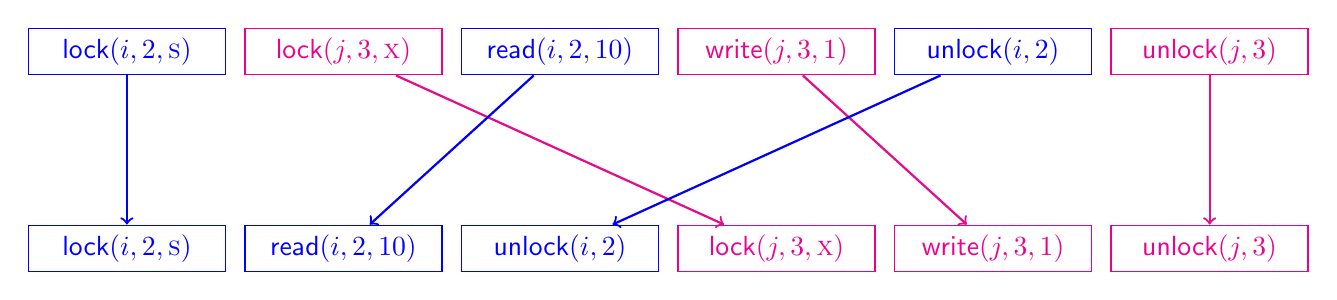
\begin{tikzpicture}[->, semithick]
		\tikzset{
		    tleft/.style= {rectangle, draw=blue, color=blue, minimum width=2.5cm},
		    tright/.style= {rectangle, draw=magenta, color=magenta, minimum width=2.5cm},
		    pleft/.style= {above, black!5!blue, thick},
		    pright/.style= {above, black!5!magenta, thick},
		}
		
		\node[tleft] (s1) at (0, 0) {$\actlock{i}{2}{\textsc{s}}$};
		\node[tright] (s2) at (2.75, 0) {$\actlock{j}{3}{\textsc{x}}$};
		\node[tleft] (s3) at (5.5, 0) {$\actread{i}{2}{10}$};
		\node[tright] (s4) at (8.25, 0) {$\actwrite{j}{3}{1}$};
		\node[tleft] (s5) at (11, 0) {$\actunlock{i}{2}$};
		\node[tright] (s6) at (13.75, 0) {$\actunlock{j}{3}$};
		
		\node[tleft] (s7) at (0,-2.5) {$\actlock{i}{2}{\textsc{s}}$};
		\node[tleft] (s8) at (2.75,-2.5) {$\actread{i}{2}{10}$};
		\node[tleft] (s9) at (5.5,-2.5) {$\actunlock{i}{2}$};
		\node[tright] (s10) at (8.25,-2.5) {$\actlock{j}{3}{\textsc{x}}$};
		\node[tright] (s11) at (11,-2.5) {$\actwrite{j}{3}{1}$};
		\node[tright] (s12) at (13.75,-2.5) {$\actunlock{j}{3}$};
		
		\draw
		(s1) edge[pleft] (s7)
		(s2) edge[pright] (s10)
		(s3) edge[pleft] (s8)
		(s4) edge[pright] (s11)
		(s5) edge[pleft] (s9)
		(s6) edge[pright] (s12);
	\end{tikzpicture}
	\captionof{figure}{A serializable trace at the top with the corresponding equivalent and serial trace.}
\end{center}

\subsubsection{Graphs}

The proof of serializability will be carried over a particular representation of traces that we introduce in this section. We utilize serialization graphs in order to describe relationships between transactions participating in a program execution.

\begin{defn}
	(Serialization graph).
	The \emph{serialization graph} of a given trace $\tau$ is a directed graph whose nodes are the identifiers of all the transactions that perform an action as part of $\tau$ and whose edges are between transactions that have ordered conflicting operations according to $\tau$.
	\begin{align*}
		\pred{SG}{\tau} &\triangleq (N, E) \\
		\text{where } N &\triangleq \{ \iota\ |\ op(\iota) \in \tau \} \\
		E &\triangleq
			\begin{aligned}
				\{
					(i, j)\ |&\ x = op(i, k) \land x' = op(j, k) \\
					&\land \pred{conflict}{x, x'} \land \tau \vDash x < x' 
				\}	
			\end{aligned}
	\end{align*}
\end{defn}

Edge connections and paths within a graph $G = (N, E)$ are described by introducing an arrow notation. We write $i \rightarrow j \in G$ to indicate that there is an edge from node $i$ to node $j$ in $E$. In the following list of statements, we make an abuse of notation to allow more expressive formulas and add a transitive closure arrow ($\rightarrow^*$) that is able to describe a path in the graph.
\[
	\begin{array}{l l}
		i \rightarrow j \in E \triangleq (i, j) \in E
			&
		i \rightarrow j \in G \triangleq i \rightarrow j \in G \downarrow_2
			\\
		i \rightarrow^1 j \in E \triangleq i \rightarrow j \in E
			&
		i \rightarrow^n j \in E \triangleq \exists t \ldotp i \rightarrow t \in E \land t \rightarrow^{n-1} \in E
			\\
		i \rightarrow^* j \in E \triangleq \exists n \ldotp i \rightarrow^n j \in E
			\ \ \ \ &
		i \rightarrow^* j \in G \triangleq i \rightarrow^* j \in G \downarrow_2
	\end{array}		
\]

Our goal is now to prove that all traces whose serialization graph contains no cyclic paths are serializable. We do this by first formally introducing the acyclic property of graphs and later the concept of a topological order of a graph.

\begin{defn}
	(Acyclic graph).
	A graph $G = (N, E)$ is \emph{acyclic} if and only if there is no path in $G$ that connects a node in $N$ to itself.
	\[
		\pred{acyclic}{G} \iff \forall a \ldotp a \in G \downarrow_1 \implies \lnot a \rightarrow^* a \in G
	\]
\end{defn}

\begin{defn}
	(Topological sort).
	A \emph{topological sort} of a graph $G = (N, E)$ is an ordered sequence of all nodes in $N$ such that if node $a$ appears before node $b$ in the sequence, then there is no path from $b$ to $a$ in $G$.
	\begin{gather*}
		t = \pred{topo}{(N, E)} \iff \\
		(\forall n \ldotp n \in t \iff n \in N) \land (\forall a, b \ldotp t \vDash a < b \implies \lnot b \rightarrow^* a \not\in E)
	\end{gather*}
\end{defn}

The following theorem establishes a key property we later need in order to prove serializability of the operational semantics introduced in Section \ref{sec:2plSemantics}. The process will in fact start by building the serialization graph of an arbitrary trace arising from \tpl\ semantics, showing that under any circumstance it is acyclic and from Theorem \ref{thm:acySer} we obtain the result needed.
\begin{thm}
	\label{thm:acySer}
	(Acyclic means serializable).
	Every trace that has a serialization graph with no cycles is serializable.
	\[
		\forall \tau \ldotp \pred{acyclic}{\pred{SG}{\tau}} \implies \pred{serializable}{\tau}
	\]
	
	\begin{proof}
	Let's assume that $\tau \in [\mathsf{Act} \times \mathds{N}]$ is a trace which includes operations coming from transactions identified with $N = \{ \iota_1, \ldots, \iota_m \}$ for a finite $m$. It follows that $N$ is also the set of nodes of $\pred{SG}{\tau}$. By our original assumption we know that $\pred{SG}{\tau}$ is acyclic. For this reason we can always find a topological sort $t = \pred{topo}{\pred{SG}{\tau}} = [t_{\iota_1}, \ldots, t_{\iota_m}]$. Let $\tau'$ be the serial trace that includes transactions (in the presented order) identified with $t_{\iota_1}, \ldots, t_{\iota_m}$ and has all of the same operations as $\tau$. Let $x = op(i, k)$ and $x' = op(j, k)$ such that $\pred{conflict}{x, x'}$ holds and $\tau \vDash x < x'$. By definition of serialization graph, $i \rightarrow j \in \pred{SG}{\tau}$. Therefore, in any topological sort of $\pred{SG}{\tau}$, $i$ must appear before $j$. As a consequence, all of $i$'s operations appear before $j$'s ones in $\tau'$ and in particular $\tau' \vDash x < x'$. By construction, $\tau'$ is serial and it contains all of $\tau$'s operations and we showed that any two conflicting operations are ordered in the same way. We can conclude that $\tau \equiv \tau'$ which implies that $\tau$ is serializable.
	\end{proof}
\end{thm}

\subsubsection{Proof}

\begin{lem}
	All read, write or alloc operations are followed by an unlock action on the same key done by the same transaction.
	\[
		\forall \tau, \iota, k, \kappa, x \ldotp
		x = op(\iota, k) \land x \in \tau \implies \left( \tau \vDash x < \actunlock{\iota}{k} \right)
	\]
\end{lem}

\begin{lem}
	All reads are preceded by the appropriate shared lock acquisition.
	\begin{gather*}
		\forall \tau, \iota, k, v, \kappa, x, n \ldotp \\
		x = (\actread{\iota}{k}{v}, n) \land x \in \tau \implies \left( \tau \vDash \actlock{\iota}{k}{\kappa} < x \land \kappa \geq \textsc{s} \right)
	\end{gather*}
\end{lem}

\begin{lem}
	All writes to a cell are preceded by the appropriate exclusive lock acquisition.
	\begin{gather*}
		\forall \tau, x, i, k, v, n \ldotp
		x = (\actwrite{i}{k}{v}, n) \land x \in \tau \implies
		\tau \vDash \actlock{i}{k}{\textsc{x}} < x
	\end{gather*}
\end{lem}

\begin{lem}
	A read or write operation accessing a cell allocated as part of the trace, must appear after the corresponding alloc action.
	\begin{gather*}
		\forall \tau, i, j, x, x', n, n', l, m, k, v, \kappa \ldotp \\
		x = (\actalloc{i}{m}{l}, n) \land x' \in \{ (\actread{j}{k}{v}, n'), (\actwrite{j}{k}{v}, n') \} \land l \leq k < l + m
		\\
		\land x \in \tau \land x' \in \tau
		\implies
		\left( \tau \vDash x < x'  \land \tau \vDash \actunlock{i}{k} < \actlock{j}{k}{\kappa} \right)
	\end{gather*}
\end{lem}

\begin{lem}
	No lock is acquired by a transaction after one gets released by the same transaction.
	\begin{gather*}
		\forall \tau, \iota, k, k', n, n', x, x', \kappa \ldotp \\
		\left( x = (\actlock{\iota}{k}{\kappa}, n) \land x' = (\actunlock{\iota}{k'}, n') \land x \in \tau \land x' 	\in \tau \right) \\
		\implies \left( \tau \vDash x < x' \right)
	\end{gather*}
\end{lem}

\begin{lem}
	If two transactions run conflicting operations on the same item, either one releases its lock before the other acquires it or vice versa.
	\begin{gather*}
		\forall \tau, i, j, k, \kappa, \kappa', x, x' \ldotp \\
		x = op(i, k) \in \tau \land x' = op(j, k) \in \tau \land \pred{conflict}{x, x'} \\
		\implies \left( \tau \vDash \actunlock{i}{k} < \actlock{j}{k}{\kappa} \right) \lor \left( \tau \vDash \actunlock{j}{k} < \actlock{i}{k}{\kappa'} \right)
	\end{gather*}
\end{lem}

\lem \label{lem:sg1}
\begin{gather*}
\forall \tau, i, j \ldotp i \rightarrow j \in \pred{SG}{\tau} \implies \\
\exists k, \kappa, x, x' \ldotp x = op(i, k) \in \tau \land x' = op(j, k) \in \tau \\
\land\ \pred{conflict}{x, x'} \land \tau \vDash \actunlock{i}{k} < \actlock{j}{k}{\kappa}
\end{gather*}
\begin{proof}
Let's pick an arbitrary trace $\tau \in [(\mathsf{Act}, \mathds{N})]$, such that $\tau = \pred{trace}{h, \emptyset, \emptyset, \mathds{P}}$ for some $h \in \mathsf{Storage}$, $\mathds{P} \in \mathsf{Prog}$ and transaction identifiers $i, j \in \mathsf{Tid}$. Now we assume that $i \rightarrow j \in \pred{SG}{\tau}$. By definition of a serialization graph built through $\mathsf{SG}$ we directly obtain that there must be two operations $x = op(i, k)$ and $x' = op(j, k)$ in $\tau$ which are conflicting, so $\pred{conflict}{x, x'}$ holds and $\tau \vDash x < x'$ (\textsc{i}).

In the case where $x = (\actalloc{i}{n}{l}, n')$ for some $n, n' \in \mathds{N}$, then we obtain the needed result from Lemma \ref{lem:allocBefore}.

Otherwise $x$ and $x'$ are conflicting read/write operations. By Lemma \ref{lem:read}, Lemma \ref{lem:write} and Lemma \ref{lem:unlock} we obtain the following, for $x_i^l = (\actlock{i}{k}{\kappa}, n_1), x_i^u = (\actunlock{i}{k}, n_2), x_j^l = (\actlock{j}{k}{\kappa'}, n_3), x_j^u = (\actunlock{j}{k}, n_4)$ and $n_1, n_2, n_3, n_4 \in \mathds{N}, \kappa, \kappa' \in \mathsf{Lock}$.
\begin{enumerate}
	\item \label{sg1.1} $\tau \vDash x_i^l < x < x_j^u$
	\item \label{sg1.2} $\tau \vDash x_j^l < x' < x_j^u$
\end{enumerate}
By Lemma \ref{lem:conflict} we know that either $\tau \vDash x_i^u < x_j^l$ or $\tau \vDash x_j^u < x_i^l$ holds. In the case where $\tau \vDash x_j^u < x_i^l$ holds, by points \ref{sg1.1} and \ref{sg1.2} we would get that $\tau \vDash x' < x$ which contradicts (\textsc{i}). Therefore it must be the case that $\tau \vDash x_i^u < x_j^l$ holds.
\end{proof}

\lem \label{lem:sg2}
\begin{gather*}
\forall \tau, i, j, n > 0 \ldotp i \rightarrow^n j \in \pred{SG}{\tau} \implies \\
\exists k, k', \kappa \ldotp op(i, k) \in \tau \land op(j, k') \in \tau \land \tau \vDash \actunlock{i}{k} < \actlock{j}{k}{\kappa}
\end{gather*}

{\parindent0pt
\begin{proof}
Let's pick an arbitrary trace $\tau \in [(\mathsf{Act}, \mathds{N})]$, such that $\tau = \pred{trace}{h, \emptyset, \emptyset, \mathds{P}}$ for some $h \in \mathsf{Storage}$, $\mathds{P} \in \mathsf{Prog}$, $n \in \mathds{Z}$ such that $n > 0$ and transaction identifiers $i, j \in \mathsf{Tid}$. We will prove the lemma by induction on $n$. \\

\textit{Base case}: $n = 1$

We assume that $i \rightarrow^1 j \in \pred{SG}{\tau}$ which, by definition, is equivalent to $i \rightarrow j \in \pred{SG}{\tau}$. By Lemma \ref{lem:sg1} we get that $\exists k, \kappa \ldotp \alpha_i(k) \in \tau \land \alpha_j(k) \in \tau \land \tau \vDash \actunlock{i}{k} < \actlock{j}{k}{\kappa}$ that concludes the proof for this case. \\

\textit{Inductive case}: $n > 1$

\textit{Inductive hypothesis}: Assume the property holds for $n$.

We now want to prove the same property for $n + 1$ so we assume that $i \rightarrow^{n+1} j \in \pred{SG}{\tau}$. By definition, we know that for $n$ and some $t \in \mathsf{Tid}$, $i \rightarrow^n t \in \pred{SG}{\tau}$ and $t \rightarrow j \in \pred{SG}{\tau}$ holds. By inductive hypothesis on $n$ we obtain that, for keys $k_1, k_2 \in \mathsf{Key}$ and lock mode $\kappa_t \in \mathsf{Lock}$, there are two operations $op(i, k_1)$ and $op(t, k_2)$ which are part of $\tau$ and that $\tau \vDash \actunlock{i}{k_1} < \actlock{t}{k_2}{\kappa_t}$ holds. By the fact that $t \rightarrow j \in \pred{SG}{\tau}$ holds and Lemma \ref{lem:sg1} we know that, for a storage key $k \in \mathsf{Key}$ and lock mode $\kappa \in \mathsf{Lock}$, there are two conflicting actions $op(t, k)$ and $op(j, k)$ inside $\tau$ such that $\tau \vDash \actunlock{t}{k} < \actlock{j}{k}{\kappa}$. By Lemma \ref{lem:2phase} we obtain that $\tau \vDash \actlock{t}{k_2}{\kappa_t} < \actunlock{t}{k}$ holds. As a consequence, it follows that $\tau \vDash \actunlock{i}{k_1} < \actlock{j}{k}{\kappa}$.
\end{proof}
}

\thm \label{thm:sgAcyclic}
\[
\forall \tau, i \ldotp i \in \pred{SG}{\tau} \downarrow_1 \implies \lnot i \rightarrow^* i \in \pred{SG}{\tau}
\]

\begin{proof}
Let's pick an arbitrary trace $\tau \in [(\mathsf{Act}, \mathds{N})]$, such that $\tau = \pred{trace}{h, \emptyset, \emptyset, \mathds{P}}$ for some $h \in \mathsf{Storage}$, $\mathds{P} \in \mathsf{Prog}$ and transaction identifier $i \in \mathsf{Tid}$. We assume that $i$ is part of the transaction identifiers in the serialization graph, i.e. $i \in \pred{SG}{\tau} \downarrow_1$. Let's also assume that the graph contains a cycle on $i$, which means that $\exists n \ldotp i \rightarrow^n i \in \pred{SG}{\tau}$. By Lemma \ref{lem:sg2} we obtain that for some keys $k, k' \in \mathsf{Key}$ and lock mode $\kappa \in \mathsf{Lock}$, $\tau \vDash \actunlock{i}{k} < \actlock{i}{k'}{\kappa}$ which contradicts Lemma \ref{lem:2phase}. Therefore, by contradiction we get that $\lnot i \rightarrow^* i \in \pred{SG}{\tau}$.
\end{proof}

\newpage

\subsection{Semantics Equivalence}

\label{sec:semEquiv}

Serializability gives us an important consistency property on the \tpl\ operational semantics that we defined. In abstract terms, it allows us to think about program executions in some sequential order, without having to consider all possible interleavings that may arise. At this point, we want to show an even stronger result which is the semantics equivalence between the semantics defined in Section \ref{sec:2plSemantics} and some \textit{atomic} operational semantics, defined in Section \ref{sec:atomicSem}, that reduce transactions in one go, as if the system stops when they begin execution and starts again when they are done. In database terms, this is referred to as \textit{strict serializability}, where, on top of order between parallel transactions, the internal program order is also preserved. The equivalence not only allows us to forget about the peculiar locking details of \tpl\ and thus only to focus on \textit{atomic} reductions, but also provides us with soundness with respect to the mCAP program logic defined in Section \ref{sec:mcapModel}. This empowers us to build mCAP proofs of programs running under the \tpl\ semantics.

The final outcome of this section will be a proof of the following statement, which says that any program that terminates, i.e. reduces to $\pskip$, under the \tpl\ operational semantics will have the same overall effect on the global storage as the same terminating program running under the \textsc{Atom} semantics and starting with the same state.
\[
	\forall h, h', S, S', \mathds{P} \ldotp
	(h, \emptyset, S, \mathds{P}) \rightarrow^* (h', \emptyset, S', \pskip) \implies 
	(h, \mathds{P}) \tred^* (h', \pskip)
\]

In order for the semantics equivalence claim to be complete, the inverse implication also needs to be established. This states that the final storage of any terminating program reduction in \textsc{Atom}, will be reachable by reducing the same program starting from the same initial state in \textsc{2pl}, where the transactions' state components are existentially quantified.
\[
	\forall h, h' \ldotp
	(h, \mathds{P}) \tred^* (h', \pskip)
	\implies
	\exists S, S' \ldotp
	(h, \emptyset, S, \mathds{P}) \rightarrow^* (h', \emptyset, S', \pskip)
\]
We do not formally prove this result given that it is trivial to understand that the \textsc{Atom} semantics can be replicated by the \tpl\ ones, simply by always chosing to reduce the same transaction until it reaches $\pskip$, without allowing concurrent interleaving. Given that we start with an empty lock manager component $\emptyset$, run transactions one after the other and each of those needs to remove its footprint from locks before terminating, no transaction will get \textit{stuck} as part of the overall reduction.

\subsubsection{Atomic semantics}

\label{sec:atomicSem}

The atomic operational semantics shown here are behaviourally equivalent to the ones presented in Section \ref{sec:mcapOpSem}. They are converted to a transition relation for clarity and in order to ease the general proof, since the \tpl\ semantics are also expressed with a comparable structure.

The rules that follow determine a relation between storages under the effect of a program. At the level of programs, they are very similar to the \tpl\ ones, a part from the absence of a lock manager or a transactions stack. These two structures are not needed here, since there is no interleaving which happens as a result of running transactions concurrently. For this reason, there is no need to globally track information about a transaction's internal execution. Note how such behaviour is obtained through the \textsc{AtExec} rule, which reduces a transaction's body at once, by running a multi-step reduction on command $\mathds{C}$ until it hits $\pskip$. Parallelism is again obtained by nondeterministically reducing one of the two programs that are composed together.

\[
(-, -) \rightarrow (-, -) : (\mathsf{Storage} \times \mathsf{Prog})^2
\]
\[\footnotesize\def\arraystretch{3.5}
	\begin{array}{c c}
		\infer[\textsc{AtTrans}]
		{
			(h, \mathds{T}) \tred (h', \pskip)
		}
		{
			(h, \mathds{T}) \tred (h', \ptdef{\pskip})
		}
		&
		\infer[\textsc{AtPSkip}]
		{
			(h, \pskip ; \mathds{P}) \tred (h, \mathds{P})
		}
		{}
		\\
		\infer[\textsc{AtPSeq}]
		{
			(h, \mathds{P}_1 ; \mathds{P}_2) \tred (h', \mathds{P}_1' ; \mathds{P}_2)
		}
		{
			(h, \mathds{P}_1) \tred (h', \mathds{P}_1')
		}
		&
		\infer[\textsc{AtPar}]
		{
			(h, \pskip \| \pskip) \tred (h, \pskip)
		}
		{}
		\\
		\infer[\textsc{AtParL}]
		{
			(h, \mathds{P}_1 \| \mathds{P}_2) \tred (h', \mathds{P}_1' \| \mathds{P}_2)
		}
		{
			(h, \mathds{P}_1) \tred (h', \mathds{P}_1')
		}
		&
		\infer[\textsc{AtParR}]
		{
			(h, \mathds{P}_1 \| \mathds{P}_2) \tred (h', \mathds{P}_1 \| \mathds{P}_2')
		}
		{
			(h, \mathds{P}_2) \tred (h', \mathds{P}_2')
		}
		\\
		\infer[\textsc{AtChoiceL}]
		{
			(h, \mathds{P}_1 + \mathds{P}_2)
			\tred
			(h, \mathds{P}_1)
		}
		{}
		&
		\infer[\textsc{AtChoiceR}]
		{
			(h, \mathds{P}_1 + \mathds{P}_2)
			\tred
			(h, \mathds{P}_2)
		}
		{}
		\\
		\infer[\textsc{AtLoop}]
		{
			(h, \mathds{P}^*)
			\tred
			(h, \pskip + (\mathds{P} ; \mathds{P}^*))
		}
		{}
		&
		\infer[\textsc{AtExec}]
		{
			(h, \ptdef{\mathds{C}})
			\tred
			(h', \ptdef{\pskip})
		}
		{
			(h, \emptyset, \mathds{C})
			\tred^*
			(h', -, \pskip)
		}
	\end{array}
\]

The atomic operational semantics of commands are defined through the rules that follow. They show the reduction of a command when executed on a storage $h$ and variable stack $s$. The rules are equivalent to the \tpl\ ones but, given the atomic setting, there is no need for a state component that determines the phase of a transaction. There are no rules concerned with locking and unlocking either, since under the atomic semantics, transactions run in concrete and real isolation without the need to be managed when accessing storage cells.

\[
(-, -, -) \tred (-, -, -) : (\mathsf{Storage} \times \mathsf{Stack} \times \mathsf{Cmd})^2
\]
\[\footnotesize\def\arraystretch{3.5}
	\begin{array}{@{\hspace*{-28pt}}c @{\hspace{2pt}} c @{}}
		\infer[\textsc{AtSkip}]
		{
			(h, s, \pskip ; \mathds{C})
			\tred
			(h, s, \mathds{C})
		}
		{}
		&
		\infer[\textsc{AtCondT}]
		{
			(h, s, \pif{\mathds{B}}{\mathds{C}_1}{\mathds{C}_2})
			\tred
			(h, s, \mathds{C}_1)
		}
		{
			\tsem{\mathds{B}}^\textsc{b} = \top
		}
		\\
		\infer[\textsc{AtSeq}]
		{
			(h, s, \mathds{C}_1 ; \mathds{C}_2)
			\tred
			(h', s', \mathds{C}_1' ; \mathds{C}_2)
		}
		{
			(h, s, \mathds{C}_1)
			\tred
			(h', s',\mathds{C}_1')
		}
		&
		\infer[\textsc{AtWrite}]
		{
			(h, s, \pmutate{\mathds{E}_1}{\mathds{E}_2})
			\tred
			(h[k \mapsto v], s, \pskip)
		}
		{
			k = \llbracket \mathds{E}_1 \rrbracket_s\ \
			k \in \pred{dom}{h}\ \
			v = \llbracket \mathds{E}_2 \rrbracket_s
		}
		\\
		\infer[\textsc{AtAssign}]
		{
			(h, s, \passign{\pvar{x}}{\mathds{E}})
			\tred
			(h, s[\pvar{x} \mapsto v], \pskip)
		}
		{
			v = \llbracket \mathds{E} \rrbracket_s
		}
		&
		\infer[\textsc{AtLoopF}]
		{
			(h, s, \ploop{\mathds{B}}{\mathds{C}})
			\tred
			(h, s, \pskip)
		}
		{
			\tsem{\mathds{B}}^\textsc{b}
		}
		\\
		\infer[\textsc{AtCondF}]
		{
			(h, s, \pif{\mathds{B}}{\mathds{C}_1}{\mathds{C}_2})
			\tred
			(h, s, \mathds{C}_2)
		}
		{
			\tsem{\mathds{B}}^\textsc{b} = \bot
		}
		&
		\infer[\textsc{AtRead}]
		{
			(h, s, \pderef{\pvar{x}}{\mathds{E}})
			\tred
			(h, s[\pvar{x} \mapsto v], \pskip)
		}
		{
			k = \llbracket \mathds{E} \rrbracket_s\ \
			k \in \pred{dom}{h}\ \
			v = h(k)
		}
		\\
		\infer[\textsc{AtLoopT}]
		{
			(h, s, \ploop{\mathds{B}}{\mathds{C}})
			\tred
			(h, s, \mathds{C}; \ploop{\mathds{B}}{\mathds{C}})
		}
		{
			\tsem{\mathds{B}}^\textsc{b} = \top
		}
	\end{array}
\]
\[\footnotesize
\infer[\textsc{AtAlloc}]
{
	(h, s, \palloc{\pvar{x}}{\mathds{E}})
	\tred
	(h[l \mapsto 0] \ldots [l + n - 1 \mapsto 0], s[\pvar{x} \mapsto l], \pskip)
}
{
	n = \llbracket \mathds{E} \rrbracket_s\ \
	l, \ldots, l + n - 1 \not\in \pred{dom}{h}
}
\]

\subsubsection{Trace equivalence}

\[
	\alpha(\iota, k) \triangleq \alpha \text{ s.t. }
	\alpha \in 
		\{
			\actread{\iota}{k}{v},
			\actwrite{\iota}{k}{v},
			\actlock{\iota}{k}{\kappa},
			\actunlock{\iota}{k}\
			|\ v \in \mathsf{Val}, \kappa \in \mathsf{Lock}
		\}
\]
\begin{align*}
	\pred{tgen}{[], h, \underline{h}, \Phi, S, \mathds{P}}
		\iff&
	h = \underline{h} \land \mathds{P} = \pskip \land \Phi = \emptyset
		\\
	\pred{tgen}{(\alpha, n) : \tau, h, \underline{h}, \Phi, S, \mathds{P}}
		\iff&
	\exists h', \Phi', S', \mathds{P}' \ldotp (h, \Phi, S, \mathds{P}) \xrightarrow{\alpha} (h', \Phi', S', \mathds{P}') \\ &\land \pred{tgen}{\tau, h', \underline{h}, \Phi', S', \mathds{P}'}
\end{align*}
\[
	\pred{absent}{\iota, k, \tau}
		\iff
	\lnot \exists v, n \ldotp (\actread{\iota}{k}{v}, n) \in \tau \lor (\actwrite{\iota}{k}{v}, n) \in \tau
\]
\[
	\pred{clean}{\tau} \iff \forall \iota, k, \kappa, n \ldotp \left( (\actlock{\iota}{k}{\kappa}, n) \in \tau \lor (\actunlock{\iota}{k}, n) \in \tau \right) \implies \lnot \pred{absent}{\iota, k, \tau}
\]

\lem \label{lem:alman} A lock on an item is not needed for any reductions a part from a read, a write or an unlock action performed by the same transaction on the same item.
\begin{gather*}
	\forall \mathds{P}, \mathds{P}', h, h', \Phi, \Phi', S, S', \alpha, i, k, v, I, \kappa \ldotp \\
	(h, \Phi, S, \mathds{P}) \xrightarrow{\alpha} (h', \Phi', S', \mathds{P}')
		\land
	(\{i\} \uplus I, \kappa) = \Phi(k)
		\land \\
	\alpha \not\in \{ \actread{i}{k}{v}, \actwrite{i}{k}{v}, \actunlock{i}{k} \}
		\implies
	\exists \Phi_m, \Phi_m', I', \kappa', \kappa'' \ldotp \\
	(h, \Phi_m, S, \mathds{P}) \xrightarrow{\alpha} (h', \Phi_m', S, \mathds{P}')
		\land
	\Phi_m = \Phi[k \mapsto (I, \kappa')]
		\land
	\Phi_m' = \Phi'[k \mapsto (I', \kappa'')]
		\land
	\kappa' \leq \textsc{s}
\end{gather*}
\begin{proof}
Let's pick arbitrary $\mathds{P}, \mathds{P}' \in \mathsf{Prog}, h, h' \in \mathsf{Storage}, \Phi, \Phi' \in \mathsf{LMan}, S, S' \in \mathsf{TState}, \alpha \in \mathsf{Act}, i \in \mathsf{Tid}, k \in \mathsf{Key}, v \in \mathsf{Val}, I \in \mathcal{P}(\mathsf{Tid}), \kappa \in \mathsf{Lock}$. We now assume that the following holds:
\begin{gather}
	\label{lem:alman1}
	(h, \Phi, S, \mathds{P}) \xrightarrow{\alpha} (h', \Phi', S', \mathds{P}')
		\land
	(\{i\} \uplus I, \kappa) = \Phi(k)
		\land
	\alpha \not\in \{ \actread{i}{k}{v}, \actwrite{i}{k}{v} \}
\end{gather}
From (\ref{lem:alman1}) we directly obtain that $\kappa \geq \textsc{s}$ given that $i$ is in the owners' set for item $k$. The proof proceeds with a case-by-case analysis on $\alpha$.
\begin{itemize}
	\item If $\alpha = \actprog$, $\alpha = \actid{\iota}$ or $\alpha = \actalloc{\iota}{n}{l}$ for some $\iota \in \mathsf{Tid}, n \in \mathds{N}, l \in \mathsf{Key}$, then the result trivially follows given that in these cases $\alpha$ has no requirementes on $\Phi$ to succesfully reduce.
	
	\item If $\alpha = \actread{j}{k'}{v'}$ for $j \in \mathsf{Tid}, k' \in \mathsf{Key}, v' \in \mathsf{Val}$ then from (\ref{lem:alman1}) we know that $i \neq j$. Next we consider the following two cases:
		\begin{itemize}
			\item If $k = k'$ then from (\ref{lem:alman1}) we obtain that, given the $\alpha$ action has succesfully reduced, $\kappa = \textsc{s}$ and $j \in I$. Therefore we can find $\kappa' = \textsc{s}, \kappa'' = \textsc{s}$ and $I' = I$.
			\item If $k \neq k'$ then $\alpha$ has no requirement on $\Phi(k)$ to succesfully reduce and the result follows.
		\end{itemize}
		
	\item If $\alpha = \actwrite{j}{k'}{v'}$ for $j \in \mathsf{Tid}, k' \in \mathsf{Key}, v' \in \mathsf{Val}$ then from (\ref{lem:alman1}) we know that $i \neq j$. Next we consider the following two cases:
		\begin{itemize}
			\item If $k = k'$ then it is not possible that $\alpha$ succesfully reduced since from (\ref{lem:alman1}) we know that $i$ was in the owners set for key $k$, then it must be the case that $k \neq k'$.
			\item If $k \neq k'$ then $\alpha$ has no requirement on $\Phi(k)$ to succesfully reduce and the result follows.
		\end{itemize}
		
	\item If $\alpha = \actlock{j}{k'}{\kappa_j}$ for some $j \in \mathsf{Tid}, k' \in \mathsf{Key}, \kappa_j \in \mathsf{Lock}$.
		\begin{itemize}
			\item If $k \neq k'$ then $\alpha$ has no requirement on $\Phi(k)$ to succesfully reduce and the result follows.
			\item If $k = k'$ and $i \neq j$ then from (\ref{lem:alman1}) we know that $\alpha$ succesfully reduced, and therefore $\kappa = \textsc{s}$ and $\kappa_j = \textsc{s}$. This also implies that we can find $\kappa' = \textsc{s}, I' = I \cup \{j\}$ and $\kappa'' = \textsc{s}$.
			\item If $k = k'$ and $i = j$ then given that $\Phi(k)$ already had $i$ as part of the owners, it must be the case that $\kappa = \textsc{s}, I = \emptyset$ and $\kappa_j = \textsc{x}$ in order for $\alpha$ to reduce as imposed by (\ref{lem:alman1}). It follows that we can find $\kappa' = \textsc{u}, I' = \{i\}$ and $\kappa'' = \textsc{x}$.
		\end{itemize}
		
	\item If $\alpha = \actunlock{j}{k'}$ for $j \in \mathsf{Tid}, k' \in \mathsf{Key}$ then from (\ref{lem:alman1}) we know that $i \neq j$. Next we consider the following two cases:
		\begin{itemize}
			\item If $k \neq k'$ then $\alpha$ has no requirement on $\Phi(k)$ to succesfully reduce and the result follows.
			\item If $k = k'$ then from (\ref{lem:alman1}) we know that $\alpha$ succesfully reduced meaning that $i$ and $j$ were holding the lock at the same time, making $\kappa = \textsc{s}, \kappa' = \textsc{s}, \kappa'' = \textsc{s}$ and $I' = I \setminus \{ i, j \}$.
		\end{itemize}
\end{itemize}
\end{proof}


\lem \label{lem:lockAbsent} Lock and unlock operations done by a transaction on items which it does not read or write can be removed without affecting the program or the global state.
\begin{gather*}
	\forall \tau, \tau', h, h', \Phi, S, \mathds{P}, n, n', \iota, k, \kappa, x, y \ldotp
		\\
	\pred{tgen}{\tau, h, h', \Phi, S, \mathds{P}} \land  \pred{absent}{\iota, k, \tau} \land x = (\actlock{\iota}{k}{\kappa}, n) \land y = (\actunlock{\iota}{k}, n') \\ \land x \in \tau \land y \in \tau
	\land \tau' = \tau \setminus \{ x, y \}
		\implies
	\pred{tgen}{\tau', h, h', \Phi, S, \mathds{P}}
\end{gather*}
\begin{proof}
Let's pick arbitrary $\tau, \tau' \in [\mathsf{Act} \times \mathds{N}], h, h' \in \mathsf{Storage}, \Phi \in \mathsf{LMan}, S \in \mathsf{TState}, \mathds{P} \in \mathds{Prog}, n, n' \in \mathds{N}, \iota \in \mathsf{Tid}, k \in \mathsf{Key}, \kappa \in \mathsf{Lock}, x, y \in \mathsf{Act} \times \mathds{N}$. We now assume that the following holds:
\begin{gather*}
	\pred{tgen}{\tau, h, h', \Phi, S, \mathds{P}} \land  \pred{absent}{\iota, k, \tau} \land x = (\actlock{\iota}{k}{\kappa}, n) \land y = (\actunlock{\iota}{k}, n') \\ \land x \in \tau \land y \in \tau
	\land \tau' = \tau \setminus \{ x, y \}
\end{gather*}
From Lemma \ref{lem:2phase} we obtain that $\tau \vDash x < y$. From the definition of $\mathsf{tgen}$ and the fact that both $x$ and $y$ are in $\tau$ it follows that $\kappa \geq \textsc{s}$ and:
\begin{gather}
	(h, \Phi, S, \mathds{P}) \rightarrow^* (h_1, \Phi_1, S_1, \mathds{P}_1) \xrightarrow{\actlock{\iota}{k}{\kappa}} (h_1', \Phi_1', S_1', \mathds{P}_1') \\ \rightarrow^* (h_2, \Phi_2, S_2, \mathds{P}_2) \xrightarrow{\actunlock{\iota}{k}} (h_2', \Phi_2', S_2', \mathds{P}_2') \rightarrow^* (h', \emptyset, S', \pskip)
\end{gather}
From the semantic interpretation of $\mathsf{lock}$ and $\mathsf{unlock}$, we know that it is the case that $h_1' = h_1, S_1' = S_1, \mathds{P}_1' = \mathds{P}_1, h_2' = h_2, S_2' = S_2, \mathds{P}_2' = \mathds{P}_2$ and $\Phi_1' = \Phi_1[k \mapsto (\{\iota\} \cup I, \kappa)], \Phi_2' = \Phi_2[k \mapsto (I', \kappa')]$ for $I, I' \in \mathcal{P}(\mathsf{Tid})$ such that $\iota \not\in I'$ and $\kappa' \leq \textsc{s}$. From the assumption that $\pred{absent}{\iota, k, \tau}$ holds, we know there is no read or write action on $k$ done by $\iota$ happening in $(h_1', \Phi_1', S_1', \mathds{P}_1') \rightarrow^* (h_2, \Phi_2, S_2, \mathds{P}_2)$ meaning that actions which need a presence of $\iota$'s lock acquisition on $k$ to succeed (i.e. read and write) are not there. From Lemma \ref{lem:alman} we obtain that all actions that are part of the sequence of reductions $(h_1', \Phi_1', S_1', \mathds{P}_1') \rightarrow^* (h_2, \Phi_2, S_2, \mathds{P}_2)$ will succesfully reduce with the $\Phi_1$ lock manager not containing $\iota$ as an owner for $k$. It follows that, for $(\alpha, n+1) \in \tau$ and $(\alpha', n'+1) \in \tau$:
\begin{gather}
	\label{lem:spur1} (h, \Phi, S, \mathds{P}) \rightarrow^* (h_1, \Phi_1, S_1, \mathds{P}_1) \xrightarrow{\alpha} (h_1'', \Phi_1'', S_1'', \mathds{P}_1'')
		\\
	\label{lem:spur2} \rightarrow^* (h_2'', \Phi_2'', S_2'',\mathds{P}_2'') \xrightarrow{\alpha'} (h_2, \Phi_2, S_2, \mathds{P}_2) \rightarrow^* (h', \emptyset, S', \pskip)
\end{gather}
From the initial assumption we also know that $\tau' = \tau \setminus \{ x, y \}$ meaning that $\tau'$ has all of $\tau$'s actions a part from the ones at position $n$ and $n'$. As a consequence we have that by following $\tau'$ up to (and not including) position $n$ we have $(h, \Phi, S, \mathds{P}) \rightarrow^* (h_1, \Phi_1, S_1, \mathds{P}_1)$. Skipping the operation at position $n$ which is not present in $\tau'$, we proceed with the one in position $n + 1$ all the way to (and not including) the one in position $n'$ to get by (\ref{lem:spur1}) and (\ref{lem:spur2}) that $(h_1, \Phi_1, S_1, \mathds{P}_1) \xrightarrow{\alpha} (h_1'', \Phi_1'', S_1'', \mathds{P}_1'') \rightarrow^* (h_2'', \Phi_2'', S_2'',\mathds{P}_2'')$ holds. Now we apply the action from position $n' + 1$ to the end in $\tau'$ to obtain $(h_2'', \Phi_2'', S_2'',\mathds{P}_2'') \xrightarrow{\alpha'} (h_2, \Phi_2, S_2, \mathds{P}_2) \rightarrow^* (h', \emptyset, S', \pskip)$. From the definition of $\mathsf{tgen}$ we can state that $\pred{tgen}{\tau', h, h', \Phi, S, \mathds{P}}$ holds as needed.
\end{proof}

\lem \label{lem:rr} The order of two consecutive reads can be swapped as long as the transactions performing them are distinct.
\begin{gather*}
	\forall \tau, \tau', h, h', \Phi, S, \mathds{P}, i, j, k, k', v, v', \alpha, \alpha', n \ldotp \\
	i \neq j \land \alpha = \actread{i}{k}{v} \land \alpha' = \actread{j}{k'}{v'} \land (\alpha, n) \in \tau \land (\alpha', n+1) \in \tau \\ \land \pred{tgen}{\tau, h, h', \Phi, S, \mathds{P}} \land \tau' = \tau \setminus \{(\alpha, n), (\alpha', n+1)\} \cup \{ (\alpha, n+1), (\alpha', n) \}
		\\	 
	 \implies \pred{tgen}{\tau', h, h', \Phi, S, \mathds{P}}
\end{gather*}
\begin{proof}
Let's pick arbitrary $\tau, \tau' \in [\mathsf{Act} \times \mathds{N}], h, h' \in \mathsf{Storage}, \Phi \in \mathsf{LMan}, S \in \mathsf{TState}, \mathds{P} \in \mathsf{Prog}, i, j \in \mathsf{Tid}, k, k' \in \mathsf{Key}, v, v' \in \mathsf{Val}, \alpha, \alpha' \in \mathsf{Act}, n \in \mathds{N}$. We assume that the following holds:
\begin{gather*}
	i \neq j \land \alpha = \actread{i}{k}{v} \land \alpha' = \actread{j}{k'}{v'} \land (\alpha, n) \in \tau \land (\alpha', n+1) \in \tau \\ \land \pred{tgen}{\tau, h, h', \Phi, S, \mathds{P}} \land \tau' = \tau \setminus \{(\alpha, n), (\alpha', n+1)\} \cup \{ (\alpha, n+1), (\alpha', n) \}
\end{gather*}
The above means that the two transactions performing the consecutive read actions $\alpha$ and $\alpha'$ are distinct and in $\tau$. Also, $\tau'$ is equivalent to $\tau$ with the $\alpha$ and $\alpha'$ actions swapped. From the definition of $\mathsf{tgen}$ we know that following the actions in $\tau$ we obtain the following:
\begin{gather}
	\label{lem:rr1} (h, \Phi, S, \mathds{P}) \rightarrow^* (h_1, \Phi_1, S_1, \mathds{P}_1) \xrightarrow{\alpha} (h_0, \Phi_0, S_0, \mathds{P}_0) \\
	\label{lem:rr2} \xrightarrow{\alpha'} (h_2, \Phi_2, S_2, \mathds{P}_2) \rightarrow^* (h', \emptyset, S, \pskip)
\end{gather}
It is now required to show that trace $\tau'$ is executing the following:
\[
	(h, \Phi, S, \mathds{P}) \rightarrow^* (h_1, \Phi_1, S_1, \mathds{P}_1) \xrightarrow{\alpha'} (h_0', \Phi_0', S_0', \mathds{P}_0') \xrightarrow{\alpha} (h_2, \Phi_2, S_2, \mathds{P}_2) \rightarrow^* (h', \emptyset, S', \pskip)
\]
Since $i \neq j$ we know that the two action labels $\alpha$ and $\alpha'$ were produced by the two transactions running in parallel executing a single step each meaning we can write $\mathds{P}_1 = \mathds{P}_i \| \mathds{P}_j$ (or equivalently $\mathds{P}_j \| \mathds{P}_i$) for some $\mathds{P}_i, \mathds{P}_j \in \mathsf{Prog}$. It follows that $\mathds{P}_2 = \mathds{P}_i' \| \mathds{P}_j'$ for $(h_1, \Phi_1, S_1, \mathds{P}_i) \xrightarrow{\alpha} (h_0, \Phi_0, S_0, \mathds{P}_i')$ and $(h_0, \Phi_0, S_0, \mathds{P}_j) \xrightarrow{\alpha'} (h_2, \Phi_2, S_2, \mathds{P}_j')$. Given the effect of the $\mathsf{read}$ action, we know that $h_1 = h_0 = h_2, \Phi_1 = \Phi_0 = \Phi_2$. We can immediately find a $h_0' = h_1 = h_2$ and a $\Phi_0' = \Phi_1 = \Phi_2$. $\mathds{P}_0'$ will be the program $\mathds{P}_1$ that has executed a step in the program where transaction $j$ resides, formally $\mathds{P}_0' = \mathds{P}_i \| \mathds{P}_j'$ for $(h_1, \Phi_1, S_1, \mathds{P}_j) \xrightarrow{\alpha'} (h_0', \Phi_0', S_0', \mathds{P}_j')$. We know that this will always succeed since the $\mathsf{read}$ action requirements on $h_0, \Phi_0$ are all satisfied by (\ref{lem:rr2}). From this, $\mathds{P}_0'$ can always reduce to $\mathds{P}_2$ by chosing to run the program in which transaction $i$ is, i.e. $\mathds{P}_i$ as part of $(h_0', \Phi_0', S_0', \mathds{P}_i) \xrightarrow{\alpha} (h_2, \Phi_2, S_2, \mathds{P}_i')$, which is possible thanks to the assumption in (\ref{lem:rr1}). Given that by assumption $i \neq j$, it must be the case that $S(i)$ and $S(j)$ are disjoint therefore the relative ordering on the updates to the local variables does not matter.
\end{proof}

\lem \label{lem:rwlu} The order of two consecutive read, write, lock or unlock operations can be swapped as long as the transactions performing them are distinct and the keys they refer to are different.
\begin{gather*}
	\forall \tau, \tau', h, h', \Phi, S, \mathds{P}, i, j, k, k', x, y, n \ldotp \\
		i \neq j \land x = \alpha(i, k) \land y = \alpha(j, k') \land k \neq k' \land (x, n) \in \tau \land (y, n+1) \in \tau \\ \land \pred{tgen}{\tau, h, h', \Phi, S, \mathds{P}} \land \tau' = \tau \setminus \{(x, n), (y, n+1)\} \cup \{ (x, n+1), (y, n) \}
		\\	 
	 \implies \pred{tgen}{\tau', h, h', \Phi, S, \mathds{P}}
\end{gather*}
\begin{proof}
Let's pick arbitrary $\tau, \tau' \in [\mathsf{Act} \times \mathds{N}], h, h' \in \mathsf{Storage}, \Phi \in \mathsf{LMan}, S \in \mathsf{TState}, \mathds{P} \in \mathsf{Prog}, i, j \in \mathsf{Tid}, k, k' \in \mathsf{Key}, x, y \in \mathsf{Act}, n \in \mathds{N}$. We assume that the following holds:
\begin{gather}
	i \neq j \land x = \alpha(i, k) \land y = \alpha(j, k') \land (x, n) \in \tau \land (y, n+1) \in \tau \\ \land \pred{tgen}{\tau, h, h', \Phi, S, \mathds{P}} \land \tau' = \tau \setminus \{(x, n), (y, n+1)\} \cup \{ (x, n+1), (y, n) \}
\end{gather}
The above means that the two transactions performing the consecutive actions $x$ and $y$ are distinct and in $\tau$. Also, $\tau'$ is equivalent to $\tau$ with the $x$ and $y$ actions swapped. From the definition of $\mathsf{tgen}$ we know that following the actions in $\tau$ we obtain the following:
\begin{gather}
	\label{lem:xy1} (h, \Phi, S, \mathds{P}) \rightarrow^* (h_1, \Phi_1, S_1, \mathds{P}_1) \xrightarrow{x} (h_0, \Phi_0, S_0, \mathds{P}_0) \\
	\label{lem:xy2} \xrightarrow{y} (h_2, \Phi_2, S_2, \mathds{P}_2) \rightarrow^* (h', \emptyset, S, \pskip)
\end{gather}
It is now required to show that trace $\tau'$ is executing the following:
\[
	(h, \Phi, S, \mathds{P}) \rightarrow^* (h_1, \Phi_1, S_1, \mathds{P}_1) \xrightarrow{y} (h_0', \Phi_0', S_0', \mathds{P}_0') \xrightarrow{x} (h_2, \Phi_2, S_2, \mathds{P}_2) \rightarrow^* (h', \emptyset, S', \pskip)
\]
Since $i \neq j$ we know that the two action labels $x$ and $y$ were produced by the two transactions running in parallel executing a single step each meaning we can write $\mathds{P}_1 = \mathds{P}_i \| \mathds{P}_j$ (or equivalently $\mathds{P}_j \| \mathds{P}_i$) for some $\mathds{P}_i, \mathds{P}_j \in \mathsf{Prog}$. It follows that $\mathds{P}_2 = \mathds{P}_i' \| \mathds{P}_j'$ for $(h_1, \Phi_1, S_1, \mathds{P}_i) \xrightarrow{x} (h_0, \Phi_0, S_0, \mathds{P}_i')$ and $(h_0, \Phi_0, S_0, \mathds{P}_j) \xrightarrow{y} (h_2, \Phi_2, S_2, \mathds{P}_j')$. We will proceed with a case-by-case analysis on $x$ and $y$ in order to find suitable $h_0'$ and $\Phi_0'$.
\begin{itemize}
	\item If $x = \actread{i}{k}{v}$ and $y = \actread{j}{k'}{v'}$ for $v, v' \in \mathsf{Val}$ then the result follows directly from Lemma \ref{lem:rr}.
	
	\item If $x = \actwrite{i}{k}{v}$ and $y = \actwrite{j}{k'}{v'}$ for $v, v' \in \mathsf{Val}$ then $h_2 = h_1[k \mapsto v][k' \mapsto v']$ since $k \neq k'$ and $\Phi_2 = \Phi_1$ meaning we can find $h_0' = h_1[k \mapsto v']$ and $\Phi_0' = \Phi_1$.
	
	\item If $x = \actread{i}{k}{v}$ and $y = \actwrite{j}{k'}{v'}$ for $v, v' \in \mathsf{Val}$ then $h_2 = h_1[k' \mapsto v']$ and $\Phi_2 = \Phi_1$ meaning we can find $h_0' = h_1[k' \mapsto v']$ and $\Phi_0' = \Phi_1$.
	
	\item If $x = \actlock{i}{k}{\kappa}$ and $y = \actunlock{j}{k'}$ for $\kappa \in \mathsf{Lock}$ then $h_2 = h_1$ and $\Phi_2 = \Phi_1[k \mapsto (I, \kappa)][k' \mapsto (I' \setminus \{j\}, \kappa')]$ since $k \neq k'$ for $I, I' \in \mathcal{P}(\mathsf{Tid})$ and $\kappa' \in \mathsf{Lock}$, meaning we can find $h_0' = h_1$ and $\Phi_0' = \Phi_1[k' \mapsto (I' \setminus \{j\}, \kappa')]$.
	
	\item If $x = \actlock{i}{k}{\kappa}$ and $y = \actlock{j}{k'}{\kappa'}$ for $\kappa, \kappa' \in \mathsf{Lock}$ then $h_2 = h_1$ and $\Phi_2 = \Phi_1[k \mapsto (I, \kappa)][k' \mapsto (I', \kappa')]$ since $k \neq k'$ for $I, I' \in \mathcal{P}(\mathsf{Tid})$ meaning we can find $h_0' = h_1$ and $\Phi_0' = \Phi_1[k' \mapsto (I', \kappa')]$.
	
	\item If $x = \actunlock{i}{k}$ and $y = \actunlock{j}{k'}$ then $h_2 = h_1$ and $\Phi_2 = \Phi_1[k \mapsto (I \setminus \{i\}, \kappa)][k' \mapsto (I' \setminus \{j\}, \kappa')]$ since $k \neq k'$ for $I, I' \in \mathcal{P}(\mathsf{Tid})$ and $\kappa, \kappa' \in \mathsf{Lock}$, meaning we can find $h_0' = h_1$ and $\Phi_0' = \Phi_1[k' \mapsto (I' \setminus \{j\}, \kappa')]$.
	
	\item If $x = \actlock{i}{k}{\kappa}$ and $y = \actread{j}{k'}{v}$ for $\kappa \in \mathsf{Lock}$ and $v \in \mathsf{Val}$ then $h_2 = h_1$ and $\Phi_2 = \Phi_1[k \mapsto (I, \kappa)]$ for $I \in \mathcal{P}(\mathsf{Tid})$, meaning we can find $h_0' = h_1$ and $\Phi_0' = \Phi_1$.
	
	\item If $x = \actlock{i}{k}{\kappa}$ and $y = \actwrite{j}{k'}{v}$ for $\kappa \in \mathsf{Lock}$ and $v \in \mathsf{Val}$ then $h_2 = h_1[k' \mapsto v]$ and $\Phi_2 = \Phi_1[k \mapsto (I, \kappa)]$ for $I \in \mathcal{P}(\mathsf{Tid})$, meaning we can find $h_0' = h_1[k \mapsto v]$ and $\Phi_0' = \Phi_1$.
	
	\item If $x = \actunlock{i}{k}$ and $y = \actread{j}{k'}{v}$ for $v \in \mathsf{Val}$ then $h_2 = h_1$ and $\Phi_2 = \Phi_1[k \mapsto (I \setminus \{j\}, \kappa)]$ for $\kappa \in \{\textsc{u}, \textsc{s}\}$ and $I \in \mathcal{P}(\mathsf{Tid})$, meaning we can find $h_0' = h_1$ and $\Phi_0' = \Phi_1$.
	
	\item If $x = \actunlock{i}{k}$ and $y = \actwrite{j}{k'}{v}$ for $v \in \mathsf{Val}$ then $h_2 = h_1[k' \mapsto v]$ and $\Phi_2 = \Phi_1[k \mapsto (I \setminus \{j\}, \kappa)]$ for $\kappa \in \{\textsc{u}, \textsc{s}\}$ and $I \in \mathcal{P}(\mathsf{Tid})$, meaning we can find $h_0' = h_1[k \mapsto v]$ and $\Phi_0' = \Phi_1$.
\end{itemize}
The inverted cases that are not included in the list can be trivially found as a consequence of the presented ones, with the appropriate substitions.

From (\ref{lem:xy1}) we obtain that $\mathds{P}_0'$ is the program $\mathds{P}_1$ that has executed a step in the program where transaction $j$ resides, formally $\mathds{P}_0' = \mathds{P}_i \| \mathds{P}_j'$ for $(h_1, \Phi_1, S_1, \mathds{P}_j) \xrightarrow{y} (h_0', \Phi_0', S_0', \mathds{P}_j')$. We know that this will always succeed since the actions act on disjoint parts of the global heap and lock manager, as showed in the case-by-case analysis above, meaning that their requirements are all satisfied by (\ref{lem:xy2}). From this, $\mathds{P}_0'$ can always reduce to $\mathds{P}_2$ by chosing to run the program in which transaction $i$ is, i.e. $\mathds{P}_i$ as part of $(h_0', \Phi_0', S_0', \mathds{P}_i) \xrightarrow{x} (h_2, \Phi_2, S_2, \mathds{P}_i')$, which is possible thanks to the assumption in (\ref{lem:xy1}). Given that by assumption $i \neq j$, it must be the case that $S(i)$ and $S(j)$ are disjoint therefore the relative ordering on the eventual updates to the local variables does not matter.
\end{proof}

\lem \label{lem:aa} The order of two consecutive allocations can be swapped as long as the transactions performing them are distinct.
\begin{gather*}
	\forall \tau, \tau', h, h', \Phi, S, \mathds{P}, i, j, m, m', l, l', \alpha, \alpha', n \ldotp \\
		i \neq j \land \alpha = \actalloc{i}{m}{l} \land \alpha' = \actalloc{j}{m'}{l'} \land (\alpha, n) \in \tau \land (\alpha', n+1) \in \tau \\ \land \pred{tgen}{\tau, h, h', \Phi, S, \mathds{P}} \land \tau' = \tau \setminus \{(\alpha, n), (\alpha', n+1)\} \cup \{ (\alpha, n+1), (\alpha', n) \}
		\\	 
	 \implies \pred{tgen}{\tau', h, h', \Phi, S, \mathds{P}}
\end{gather*}
\begin{proof}
Let's pick arbitrary $\tau, \tau' \in [\mathsf{Act} \times \mathds{N}], h, h' \in \mathsf{Storage}, \Phi \in \mathsf{LMan}, S \in \mathsf{TState}, \mathds{P} \in \mathsf{Prog}, i, j \in \mathsf{Tid}, l, l' \in \mathsf{Key}, \alpha, \alpha' \in \mathsf{Act}, n, m, m' \in \mathds{N}$. We assume that the following holds:
\begin{gather}
	i \neq j \land \alpha = \actalloc{i}{m}{l} \land \alpha' = \actalloc{j}{m'}{l'} \land (\alpha, n) \in \tau \land (\alpha', n+1) \in \tau \\ \land \pred{tgen}{\tau, h, h', \Phi, S, \mathds{P}} \land \tau' = \tau \setminus \{(\alpha, n), (\alpha', n+1)\} \cup \{ (\alpha, n+1), (\alpha', n) \}
\end{gather}
The above means that the two transactions performing the consecutive allocation actions $\alpha$ and $\alpha'$ are distinct and in $\tau$. Also, $\tau'$ is equivalent to $\tau$ with the $\alpha$ and $\alpha'$ actions swapped. From the definition of $\mathsf{tgen}$ we know that following the actions in $\tau$ we obtain the following:
\begin{gather}
	\label{lem:aa1} (h, \Phi, S, \mathds{P}) \rightarrow^* (h_1, \Phi_1, S_1, \mathds{P}_1) \xrightarrow{\alpha} (h_0, \Phi_0, S_0, \mathds{P}_0) \\
	\label{lem:aa2} \xrightarrow{\alpha'} (h_2, \Phi_2, S_2, \mathds{P}_2) \rightarrow^* (h', \emptyset, S, \pskip)
\end{gather}
It is now required to show that trace $\tau'$ is executing the following:
\[
	(h, \Phi, S, \mathds{P}) \rightarrow^* (h_1, \Phi_1, S_1, \mathds{P}_1) \xrightarrow{\alpha'} (h_0', \Phi_0', S_0', \mathds{P}_0') \xrightarrow{\alpha} (h_2, \Phi_2, S_2, \mathds{P}_2) \rightarrow^* (h', \emptyset, S', \pskip)
\]
Since $i \neq j$ we know that the two action labels $\alpha$ and $\alpha'$ were produced by the two transactions running in parallel executing a single step each meaning we can write $\mathds{P}_1 = \mathds{P}_i \| \mathds{P}_j$ (or equivalently $\mathds{P}_j \| \mathds{P}_i$) for some $\mathds{P}_i, \mathds{P}_j \in \mathsf{Prog}$. It follows that $\mathds{P}_2 = \mathds{P}_i' \| \mathds{P}_j'$ for $(h_1, \Phi_1, S_1, \mathds{P}_i) \xrightarrow{\alpha} (h_0, \Phi_0, S_0, \mathds{P}_i')$ and $(h_0, \Phi_0, S_0, \mathds{P}_j) \xrightarrow{\alpha'} (h_2, \Phi_2, S_2, \mathds{P}_j')$. Given the effect of the $\mathsf{alloc}$ action, we know that $\Phi_2 = \Phi_1 = \Phi_0$. We can immediately find a $\Phi_0' = \Phi_1 = \Phi_2$. We also know that $\{l, \ldots, l + n - 1\} \subseteq \pred{dom}{h_0}$ and in order for $\actalloc{j}{n'}{l'}$ to suceed, which it does by (\ref{lem:aa2}), $\{l', \ldots, l' + n' - 1\} \cap \pred{dom}{h_0} \equiv \emptyset$ which means that the two ranges of memory locations are disjoint. As a consequence the order of allocation does not matter in terms of reaching the final heap $h_2$; our $h_0'$ will therefore be $h_1[l' \mapsto 0]\ldots[l' + n' - 1 \mapsto 0]$. $\mathds{P}_0'$ will be the program $\mathds{P}_1$ that has executed a step in the program where transaction $j$ resides, formally $\mathds{P}_0' = \mathds{P}_i \| \mathds{P}_j'$ for $(h_1, \Phi_1, S_1, \mathds{P}_j) \xrightarrow{\alpha'} (h_0', \Phi_0', S_0', \mathds{P}_j')$. We know that this will always succeed since the $\mathsf{alloc}$ action requirements are all satisfied by (\ref{lem:aa2}). From this, $\mathds{P}_0'$ can always reduce to $\mathds{P}_2$ by chosing to run the program in which transaction $i$ is, i.e. $\mathds{P}_i$ as part of $(h_0', \Phi_0', S_0', \mathds{P}_i) \xrightarrow{\alpha} (h_2, \Phi_2, S_2, \mathds{P}_i')$, which is possible thanks to the assumption in (\ref{lem:aa1}). Given that by assumption $i \neq j$, it must be the case that $S(i)$ and $S(j)$ are disjoint therefore the relative ordering on the updates to the local variables does not matter.
\end{proof}

\lem \label{lem:ax} The order of an allocation followed by a read, write, lock or unlock can be swapped as long as the transactions performing them are distinct and the keys accessed are not part of the ones created by the allocation.
\begin{gather*}
	\forall \tau, \tau', h, h', \Phi, S, \mathds{P}, i, j, k, x, y, n, m, l \ldotp \\
		i \neq j \land x = \alpha(j, k) \land y = \actalloc{i}{m}{l} \land (x, n) \in \tau \land (y, n+1) \in \tau \land (k < l \lor k \geq l + n) \\ \land \pred{tgen}{\tau, h, h', \Phi, S, \mathds{P}} \land \tau' = \tau \setminus \{(x, n), (y, n+1)\} \cup \{ (x, n+1), (y, n) \}
		\\	 
	 \implies \pred{tgen}{\tau', h, h', \Phi, S, \mathds{P}}
\end{gather*}
\begin{proof}
Let's pick arbitrary $\tau, \tau' \in [\mathsf{Act} \times \mathds{N}], h, h' \in \mathsf{Storage}, \Phi \in \mathsf{LMan}, S \in \mathsf{TState}, \mathds{P} \in \mathsf{Prog}, i, j \in \mathsf{Tid}, k, l \in \mathsf{Key}, x, y \in \mathsf{Act}, n, m \in \mathds{N}$. We assume that the following holds:
\begin{gather*}
	i \neq j \land x = \alpha(j, k) \land y = \actalloc{i}{m}{l} \land (x, n) \in \tau \land (y, n+1) \in \tau \land (k < l \lor k \geq l + n) \\ \land \pred{tgen}{\tau, h, h', \Phi, S, \mathds{P}} \land \tau' = \tau \setminus \{(x, n), (y, n+1)\} \cup \{ (x, n+1), (y, n) \}
\end{gather*}
The above means that the two transactions performing the consecutive actions $x$ and $y$ are distinct and in $\tau$. Also, $\tau'$ is equivalent to $\tau$ with the $x$ and $y$ actions swapped. From the definition of $\mathsf{tgen}$ we know that following the actions in $\tau$ we obtain the following:
\begin{gather}
	\label{lem:ax1} (h, \Phi, S, \mathds{P}) \rightarrow^* (h_1, \Phi_1, S_1, \mathds{P}_1) \xrightarrow{x} (h_0, \Phi_0, S_0, \mathds{P}_0) \\
	\label{lem:ax2} \xrightarrow{y} (h_2, \Phi_2, S_2, \mathds{P}_2) \rightarrow^* (h', \emptyset, S, \pskip)
\end{gather}
It is now required to show that trace $\tau'$ is executing the following:
\[
	(h, \Phi, S, \mathds{P}) \rightarrow^* (h_1, \Phi_1, S_1, \mathds{P}_1) \xrightarrow{y} (h_0', \Phi_0', S_0', \mathds{P}_0') \xrightarrow{x} (h_2, \Phi_2, S_2, \mathds{P}_2) \rightarrow^* (h', \emptyset, S', \pskip)
\]
Since $i \neq j$ we know that the two action labels $x$ and $y$ were produced by the two transactions running in parallel executing a single step each meaning we can write $\mathds{P}_1 = \mathds{P}_i \| \mathds{P}_j$ (or equivalently $\mathds{P}_j \| \mathds{P}_i$) for some $\mathds{P}_i, \mathds{P}_j \in \mathsf{Prog}$. It follows that $\mathds{P}_2 = \mathds{P}_i' \| \mathds{P}_j'$ for $(h_1, \Phi_1, S_1, \mathds{P}_i) \xrightarrow{x} (h_0, \Phi_0, S_0, \mathds{P}_i')$ and $(h_0, \Phi_0, S_0, \mathds{P}_j) \xrightarrow{y} (h_2, \Phi_2, S_2, \mathds{P}_j')$. Given the effect of the $\mathsf{alloc}$ action, we know that $\Phi_2 = \Phi_1 = \Phi_0$. Given the effect of the $\mathsf{alloc}$ action, we know that $\Phi_2 = \Phi_1 = \Phi_0$ and $h_0 = h_1[l \mapsto 0]\ldots[l + n - 1 \mapsto 0]$. In order to find $h_0'$ and $\Phi_0'$, we now proceed with a case-by-case analysis on the kind of action $x$.
\begin{itemize}
	\item If $x = \actread{j}{k}{v}$ for $v \in \mathsf{Val}$ then $h_2 = h_1$ and $\Phi_2 = \Phi_1$ meaning we can find $h_0' = h_1$ and $\Phi_0' = \Phi_1$.
	
	\item If $x = \actwrite{j}{k}{v}$ for $v \in \mathsf{Val}$ then $h_2 = h_1[k \mapsto v]$ and $\Phi_2 = \Phi_1$ meaning we can find $h_0' = h_1[k \mapsto v]$ and $\Phi_0' = \Phi_1$.
	
	\item If $x = \actlock{j}{k}{\kappa}$ for some $\kappa \in \mathsf{Lock}$ then $h_2 = h_1$ and $\Phi_2 = \Phi_1[k \mapsto (I, \kappa)]$ meaning we can find $h_0' = h_1$ and $\Phi_0' = \Phi_1[k \mapsto (I, \kappa)]$ for $I \in \mathcal{P}(\mathsf{Tid})$.
	
	\item If $x = \actunlock{j}{k}$ then $h_2 = h_1$ and $\Phi_2 = \Phi_1[k \mapsto (I \setminus \{j\}, \kappa)]$ for $I \in \mathcal{P}(\mathsf{Tid})$ and $\kappa \in \{\textsc{u}, \textsc{s}\}$ meaning we can find $h_0' = h_1$ and $\Phi_0' = \Phi_1[k \mapsto (I \setminus \{j\}, \kappa)]$.
\end{itemize}
$\mathds{P}_0'$ will be the program $\mathds{P}_1$ that has executed a step in the program where transaction $j$ resides, formally $\mathds{P}_0' = \mathds{P}_i \| \mathds{P}_j'$ for $(h_1, \Phi_1, S_1, \mathds{P}_j) \xrightarrow{y} (h_0', \Phi_0', S_0', \mathds{P}_j')$. We know that this will always succeed since the $\mathsf{alloc}$ action requirements are all satisfied by (\ref{lem:ax2}). From this, $\mathds{P}_0'$ can always reduce to $\mathds{P}_2$ by chosing to run the program in which transaction $i$ is, i.e. $\mathds{P}_i$ as part of $(h_0', \Phi_0', S_0', \mathds{P}_i) \xrightarrow{x} (h_2, \Phi_2, S_2, \mathds{P}_i')$, which is possible thanks to the assumption in (\ref{lem:ax1}). Given that by assumption $i \neq j$, it must be the case that $S(i)$ and $S(j)$ are disjoint therefore the relative ordering on the updates to the local variables does not matter.
\end{proof}

\lem \label{lem:idx} The order of an $\mathsf{id}$ operation followed by any other action performed by a different transaction can be swapped.
\begin{gather*}
	\forall \tau, \tau', h, h', \Phi, S, \mathds{P}, i, j, x, y, n \ldotp \\
		i \neq j \land x = \actid{i} \land y = \alpha(j) \land (x, n) \in \tau \land (y, n+1) \in \tau \\ \land \pred{tgen}{\tau, h, h', \Phi, S, \mathds{P}} \land \tau' = \tau \setminus \{(x, n), (y, n+1)\} \cup \{ (x, n+1), (y, n) \}
		\\	 
	 \implies \pred{tgen}{\tau', h, h', \Phi, S, \mathds{P}}
\end{gather*}
Let's pick arbitrary $\tau, \tau' \in [\mathsf{Act} \times \mathds{N}], h, h' \in \mathsf{Storage}, \Phi \in \mathsf{LMan}, S \in \mathsf{TState}, \mathds{P} \in \mathsf{Prog}, i, j \in \mathsf{Tid}, x, y \in \mathsf{Act}, n \in \mathds{N}$. We assume that the following holds:
\begin{gather*}
	i \neq j \land x = \actid{i} \land y = \alpha(j) \land (x, n) \in \tau \land (y, n+1) \in \tau \land (k < l \lor k \geq l + n) \\ \land \pred{tgen}{\tau, h, h', \Phi, S, \mathds{P}} \land \tau' = \tau \setminus \{(x, n), (y, n+1)\} \cup \{ (x, n+1), (y, n) \}
\end{gather*}
The above means that the two transactions performing the consecutive actions $x$ and $y$ are performed by distinct transactions and in $\tau$. Also, $\tau'$ is equivalent to $\tau$ with the $x$ and $y$ actions swapped. From the definition of $\mathsf{tgen}$ we know that following the actions in $\tau$ we obtain the following:
\begin{gather}
	\label{lem:idx1} (h, \Phi, S, \mathds{P}) \rightarrow^* (h_1, \Phi_1, S_1, \mathds{P}_1) \xrightarrow{x} (h_0, \Phi_0, S_0, \mathds{P}_0) \\
	\label{lem:idx2} \xrightarrow{y} (h_2, \Phi_2, S_2, \mathds{P}_2) \rightarrow^* (h', \emptyset, S, \pskip)
\end{gather}
It is now required to show that trace $\tau'$ is executing the following:
\[
	(h, \Phi, S, \mathds{P}) \rightarrow^* (h_1, \Phi_1, S_1, \mathds{P}_1) \xrightarrow{y} (h_0', \Phi_0', S_0', \mathds{P}_0') \xrightarrow{x} (h_2, \Phi_2, S_2, \mathds{P}_2) \rightarrow^* (h', \emptyset, S', \pskip)
\]
Since $i \neq j$ we know that the two action labels $x$ and $y$ were produced by the two transactions running in parallel executing a single step each meaning we can write $\mathds{P}_1 = \mathds{P}_i \| \mathds{P}_j$ (or equivalently $\mathds{P}_j \| \mathds{P}_i$) for some $\mathds{P}_i, \mathds{P}_j \in \mathsf{Prog}$. It follows that $\mathds{P}_2 = \mathds{P}_i' \| \mathds{P}_j'$ for $(h_1, \Phi_1, S_1, \mathds{P}_i) \xrightarrow{x} (h_0, \Phi_0, S_0, \mathds{P}_i')$ and $(h_0, \Phi_0, S_0, \mathds{P}_j) \xrightarrow{y} (h_2, \Phi_2, S_2, \mathds{P}_j')$. Given the effect of the $\mathsf{id}$ action, we know that $h_1 = h_0, \Phi_1 = \Phi_0, S_1 = S_0$ meaning that $y$ reduced succesfully as per (\ref{lem:idx2}), with a configuration equivalent to the one after $x$ reduced. It follows that we can find $h_0' = h_1, \Phi_0' = \Phi_1, S_0' = S_1$.

$\mathds{P}_0'$ will be the program $\mathds{P}_1$ that has executed a step in the program where transaction $j$ resides, formally $\mathds{P}_0' = \mathds{P}_i \| \mathds{P}_j'$ for $(h_1, \Phi_1, S_1, \mathds{P}_j) \xrightarrow{y} (h_0', \Phi_0', S_0', \mathds{P}_j')$. We know that this will always succeed since the $\mathsf{alloc}$ action requirements are all satisfied by (\ref{lem:idx2}). From this, $\mathds{P}_0'$ can always reduce to $\mathds{P}_2$ by chosing to run the program in which transaction $i$ is, i.e. $\mathds{P}_i$ as part of $(h_0', \Phi_0', S_0', \mathds{P}_i) \xrightarrow{x} (h_2, \Phi_2, S_2, \mathds{P}_i')$, which is possible thanks to the assumption in (\ref{lem:idx1}).


\subsubsection{Strict total order}

Given that we want to be able to compare traces produced under the \tpl\ operational semantics, to the ones achieved from the \textsc{Atom} one, we need to establish a strict total order on the transactions that appear in a trace. This enables us to effectively simulate a serial reduction, as we know that, from an abstract point of view, there is a precise order of transaction where one \textit{happens before} another.

The serialization graph structure, which was formalised in Definition \ref{defn:sg}, implicitly gives us a relation on the transactions participating to a given trace through its edges. The latter is in fact a partial order relation on the transaction identifiers which represents the set of ordered conflicts inside of a trace. It is acyclic as shown in Theorem \ref{thm:sgAcyclic} and therefore a great starting point from which to build the total order we need.

\begin{defn}
	(Reflexive image).
	The reflexive image of a set $X$, written $\pred{Id}{X}$, is defined as:
	\[
		\pred{Id}{X} = \{ (x, x)\ |\ x \in X \}
	\]
\end{defn}

\begin{defn}
	(Reflexive closure).
	The reflexive closure of a given relation $R$ on a set $X$, written $R^\mathsf{id}$, is defined as:
	\[
		R^\mathsf{id} = R \cup \pred{Id}{X}
	\]
\end{defn}

\begin{defn}
	(\tpl\ Transactions order)
	\begin{align*}
		\text{let } (N, E) = \pred{SG}{\tau} \text{ in }
		\sqsubset_0 &= E^* \\
		\sqsubset_{n + 1} &=\ \sqsubset_n \cup \left( \sqsubset_n^\mathsf{id} ; \{ (i, j) \} ; \sqsubset_n^\mathsf{id} \right) \\
		&\text{where } i, j \in N \text{ and } i < j \\
		&\text{and } i \not\sqsubset_n j \text{ and } j \not\sqsubset_n i
	\end{align*}
\end{defn}

\begin{thm}
	\label{thm:totOrder}
	(Order of transactions).
	The $\sqsubset$ relation is a strict total order on the set of transactions $N$ in $(N, E) = \pred{SG}{\tau}, \tau = \pred{trace}{h, \emptyset, \emptyset, \mathds{P}}, \mathds{P} \in \mathsf{Prog}, h \in \mathsf{Storage}$.

	\begin{proof}
	In order to show the theorem, we are required to prove that for all $a, b, c \in N$:
	\begin{itemize}
		\item (Irreflexivity). $a \not\sqsubset a$
		\item (Asymmetry). If $a \sqsubset b$ then $b \not\sqsubset a$
		\item (Transitivity). If $a \sqsubset b$ and $b \sqsubset c$ then $a \sqsubset c$
		\item (Totality). $a \sqsubset b$ or $b \sqsubset a$ or $a = b$
	\end{itemize}
	
	Let's pick an arbitrary program $\mathds{P} \in \mathsf{Prog}$, initial storage $h \in \mathsf{Storage}$ and get a trace out of it $\tau = \pred{trace}{h, \emptyset, \emptyset, \mathds{P}}$. We now consider the incrementally built $\sqsubset$ relation on $N$, where $(N, E) = \pred{SG}{\tau}$. \\
	
	(Irreflexivity). The proof follows by induction on the number of $\sqsubset$ relation construction steps, $n$. Let's pick an arbitrary transaction identifier $a \in N$.
	
	{\parindent0pt
	\textit{Base case}: $n = 0$
	
	\textit{To show}: $a \not\sqsubset_0 a$
	
	By definition we know that $\sqsubset_0 = E^*$, i.e. the transitive closure on the edges of the serialization graph $\pred{SG}{\tau}$. We directly obtain that $a \not\sqsubset_0 a$ from Theorem \ref{thm:sgAcyclic}. \\
	
	\textit{Inductive case}: $n > 0$
	
	\textit{Inductive hypothesis}: $a \not\sqsubset_n a$
	
	\textit{To show}: $a \not\sqsubset_{n+1} a$
	
	Let's assume that $a \sqsubset_{n+1} a$ and by definition we know it means that, for some $i, j \in N$ such that $i < j, i \not\sqsubset_n j, j \not\sqsubset_n i$ we have:
	\[
		(a, a) \in \sqsubset_n \cup \left( \sqsubset_n^\mathsf{id} ; \{ (i, j) \} ; \sqsubset_n ^\mathsf{id} \right)
	\]
	and by I.H. we can rewrite it as $(a, a) \in \left( \sqsubset_n^\mathsf{id} ; \{ (i, j) \} ; \sqsubset_n ^\mathsf{id} \right)$ given we assumed that $\sqsubset_n$ is irreflexive. It follows that it must be the case that $(a, i)$ and $(j, a)$ are in $\sqsubset_n^\mathsf{id}$ and moreover they must be in $\sqsubset_n$ given that $i < j$ and therefore $i \neq j$. By transitivity of $\sqsubset_n$, there must be a $(j, i) \in \sqsubset_n$. By contradiction we state that $a \not\sqsubset_{n+1} a$. \\
	}
	
	(Asymmetry). The proof follows by induction on the number of $\sqsubset$ relation construction steps, $n$. Let's pick arbitrary transaction identifiers $a, b \in N$.
	
	{\parindent0pt
	\textit{Base case}: $n = 0$
	
	\textit{To show}: $a \sqsubset_0 b \implies b \not\sqsubset_0 a$
	
	By definition we know that $\sqsubset_0 = E^*$, i.e. the transitive closure on the edges of the serialization graph $\pred{SG}{\tau}$. Let's assume that $a \sqsubset_0 b$ meaning that $a \rightarrow^* b \in E$. We directly obtain that $b \not\sqsubset_0 a$ from Theorem \ref{thm:sgAcyclic}. \\
	
	\textit{Inductive case}: $n > 0$
	
	\textit{Inductive hypothesis}: $a \sqsubset_n b \implies b \not\sqsubset_n a$
	
	\textit{To show}: $a \sqsubset_{n + 1} b \implies b \not\sqsubset_{n + 1} a$
	
	Let's assume that $a \sqsubset_{n + 1} b$ and by definition we know it means that, for some $i, j \in N$ such that $i < j, i \not\sqsubset_n j, j \not\sqsubset_n i$ we have:
	\[
		(a, b) \in \sqsubset_n \cup \left( \sqsubset_n^\mathsf{id} ; \{ (i, j) \} ; \sqsubset_n ^\mathsf{id} \right)
	\]
	\begin{itemize}
		\item If $a \sqsubset_n b$ we know by I.H. that $b \not\sqsubset_n a$. Let's instead assume that $(b, a) \in \left( \sqsubset_n^\mathsf{id} ; \{ (i, j) \} ; \sqsubset_n ^\mathsf{id} \right)$ from which it follows that there is a $(b, i) \in \sqsubset_n^\mathsf{id}$ and $(j, a) \in \sqsubset_n^\mathsf{id}$. By transitivity of $\sqsubset_n$ we obtain that $(j, i) \in \sqsubset_n^\mathsf{id}$ and moreover that $j \sqsubset_n i$ since $i \neq j$ as $i < j$. By contradiction we obtain that $(b, a) \not\in \left( \sqsubset_n^\mathsf{id} ; \{ (i, j) \} ; \sqsubset_n ^\mathsf{id} \right)$. We conclude that $b \not\sqsubset_{n + 1} a$.
		\item If $(a, b) \in \left( \sqsubset_n^\mathsf{id} ; \{ (i, j) \} ; \sqsubset_n ^\mathsf{id} \right)$ which means there is a $(a, i) \in \sqsubset_n^\mathsf{id}$ and $(j, b) \in \sqsubset_n^\mathsf{id}$. Let's now assume that $(b, a) \in \left( \sqsubset_n^\mathsf{id} ; \{ (i, j) \} ; \sqsubset_n ^\mathsf{id} \right)$ meaning that there is a $(b, i) \in \sqsubset_n^\mathsf{id}$ and $(j, a) \in \sqsubset_n^\mathsf{id}$. By transitivity of $\sqsubset_n$ we obtain that $(j, i) \in \sqsubset_n^\mathsf{id}$ and moreover that $j \sqsubset_n i$ since $i \neq j$ as $i < j$. By contradiction we obtain that $(b, a) \not\in \left( \sqsubset_n^\mathsf{id} ; \{ (i, j) \} ; \sqsubset_n ^\mathsf{id} \right)$. We now assume that $b \sqsubset_n a$ which implies that $(b, a) \in \sqsubset_n^\mathsf{id}$. By transitivity of $\sqsubset_n$ we obtain that $(j, i) \in \sqsubset_n^\mathsf{id}$ and moreover that $j \sqsubset_n i$ since $i \neq j$ as $i < j$. By contradiction we obtain that $(b, a) \not\in \sqsubset_n$. We conclude that $b \not\sqsubset_{n + 1} a$.
	\end{itemize}
	}
	
	(Transitivity). We are required to show that $\forall m \geq 1 \ldotp \sqsubset^m\ \subseteq\ \sqsubset$ The proof follows by induction on the number of self-composition steps, $m$.
	
	{\parindent0pt
	\textit{Base case}: $m = 1$
	
	\textit{To show}: $\sqsubset^1\ \subseteq\ \sqsubset$ \\
	
	The result follows directly by definition $\sqsubset^1\ =\ \sqsubset\ \subseteq\ \sqsubset$. \\
	
	\textit{Inductive case}: $m > 1$
	
	\textit{Inductive hypothesis}: $\sqsubset^m\ \subseteq\ \sqsubset$
	
	\textit{To show}: $\sqsubset^{m + 1}\ \subseteq\ \sqsubset$
	\begin{align*}
		\sqsubset^{m + 1}
		&=\ \sqsubset^m ; \sqsubset \text{ by associativity} \\
		&\subseteq\ \sqsubset ; \sqsubset \text{ by I.H.} \\
		&=\ \sqsubset^2 \text{by definition} \\
		&\subseteq\ \sqsubset \text{ by Lemma \ref{lem:total2}}
	\end{align*}
	}
	
	(Totality). Let's pick arbitrary transaction identifiers $a, b \in N$ (\textsc{i}) for a finite $N$ and build the $\sqsubset$ relation on it until convergence, i.e. in a finite number of steps. If $(a, b) \in E^*$ or $(b, a) \in E*$ then we know that either $a \sqsubset b$ or $b \sqsubset a$ holds. On the other hand if there is no edge connecting $a$ to $b$ or $b$ to $a$ in $E^*$ (\textsc{ii}) then:
	\begin{itemize}
		\item If $a = b$ then by irreflexivity of $\sqsubset$ we are done, as totality is met.
		\item Without loss of generality, we say that $a < b$ (\textsc{iii}). Given that the construction of $\sqsubset$ terminated in some $m > 0$ steps (being $N$ a finite set), by (\textsc{i}), (\textsc{ii}) and (\textsc{iii}) we know that there must exist a construction step $n$ such that $0 < n < m$ where the tuple $(a, b)$ was inserted in the relation given that $\sqsubset_{n-1} \cup \left( \sqsubset_{n-1}^\mathsf{id} ; \{(a,b)\} ; \sqsubset_{n-1}^\mathsf{id} \right) \implies a \sqsubset_n b \implies a \sqsubset b$. 
	\end{itemize}
	\end{proof}
\end{thm}
	
\begin{lem}
	\label{lem:total2}
	Given a serialization graph $(N, E) = \pred{SG}{\tau}$ for $\tau = \pred{trace}{h, \emptyset, \emptyset, \mathds{P}}, \mathds{P} \in \mathsf{Prog}, h \in \mathsf{Storage}$, and the $\sqsubset$ relation on the set $N$ we say that $\sqsubset^2\ \subseteq\ \sqsubset$.
	
	{\parindent0pt
	\begin{proof}
	We proceed by induction on the number of $\sqsubset$ construction steps, $n$. \\
	
	\textit{Base case}: $n = 0$
	
	\textit{To show}: $\sqsubset_0^2\ \subseteq\ \sqsubset_0$
	
	By definition we know that $\sqsubset_0 = E^*$, i.e. the transitive closure on the edges of the serialization graph $\pred{SG}{\tau}$. It follows that by definition of transitive closure, $\sqsubset_0^2\ = E^* ; E^* = E^*$ meaning that $\sqsubset_0^2\ \subseteq\ \sqsubset_0$. \\
	
	\textit{Inductive case}: $n > 0$
	
	\textit{Inductive hypothesis}: $\sqsubset_n^2\ \subseteq\ \sqsubset_n$
	
	\textit{To show}: $\sqsubset_{n + 1}^2\ \subseteq\ \sqsubset_{n + 1}$
	
	We can rewrite the formula to be proven as the following, for some $i, j \in N$ such that $i < j, i \not\sqsubset_n j, j \not\sqsubset_n i$:
	\begin{align}
		\left( \sqsubset_n \cup \underbrace{\left( \sqsubset_n^\mathsf{id} ; \{ (i, j) \} ; \sqsubset_n^\mathsf{id} \right)}_{R} \right) ; \left( \sqsubset_n \cup \left( \sqsubset_n^\mathsf{id} ; \{ (i, j) \} ; \sqsubset_n^\mathsf{id} \right) \right) &\subseteq \sqsubset_{n + 1} \\
		\label{thm:total1} \sqsubset_n ; \sqsubset_n \cup \sqsubset_n ; R \cup R ; \sqsubset_n \cup R ; R &\subseteq\ \sqsubset_{n + 1} \text{ by distributivity}
	\end{align}
	It now suffices to show that each unioned set in the L.H.S. of (\ref{thm:total1}) is a subset of $\sqsubset_{n + 1}$ itself.
	\begin{itemize}
		\item \textit{To show}: $\sqsubset_n ; \sqsubset_n\ \subseteq\ \sqsubset_{n + 1}$
			\begin{align}
				\sqsubset_n ; \sqsubset_n\ &=\ \sqsubset_n^2 \\
				\text{by I.H.}&\subseteq\ \sqsubset_n\ \subseteq\ \sqsubset_{n + 1}
			\end{align}
		\item \textit{To show}: $\sqsubset_n ; \left( \sqsubset_n^\mathsf{id} ; \{ (i, j) \} ; \sqsubset_n^\mathsf{id} \right) \subseteq\ \sqsubset_{n + 1}$
			\begin{align}
				S  &=\ \sqsubset_n ; \sqsubset_n^\mathsf{id} \\
					&=\ \sqsubset_n ; \left( \sqsubset_n \cup\ \pred{Id}{N} \right) \text{by definition} \\
					&=\ \sqsubset_n ; \sqsubset_n \cup \sqsubset_n ; \pred{Id}{N} \\
					&=\ \sqsubset_n^2 \cup \sqsubset_n \\
					&\subseteq\ \sqsubset_n \text{by I.H.} \\
					\label{thm:total2} &\subseteq\ \sqsubset_n^\mathsf{id} \text{by definition} \\
				\sqsubset_n ; \left( \sqsubset_n^\mathsf{id} ; \{ (i, j) \} ; \sqsubset_n^\mathsf{id} \right) &= \left( \sqsubset_n ; \sqsubset_n^\mathsf{id} ; \{ (i, j) \} \right) ; \sqsubset_n^\mathsf{id} \text{ by associativity} \\
				&= \left( S ; \{ (i, j) \} \right) ; \sqsubset_n^\mathsf{id} \text{ by associativity} \\
				&\subseteq\ \sqsubset_n^\mathsf{id} ; \{ (i, j) \} ; \sqsubset_n^\mathsf{id} \text{by (\ref{thm:total2})} \\
				&\subseteq\ \sqsubset_{n + 1}
			\end{align}
		\item \textit{To show}: $\left( \sqsubset_n^\mathsf{id} ; \{ (i, j) \} ; \sqsubset_n^\mathsf{id} \right) ; \sqsubset_n \subseteq\ \sqsubset_{n + 1}$
			\begin{align}
				S' &=\ \sqsubset_n^\mathsf{id} ; \sqsubset_n \\
					&= \left( \sqsubset_n \cup\ \pred{Id}{N} \right) ; \sqsubset_n \text{by definition} \\
					&=\ \sqsubset_n ; \sqsubset_n \cup\ \pred{Id}{N} ; \sqsubset_n \\
					&=\ \sqsubset_n^2 \cup \sqsubset_n \\
					&\subseteq\ \sqsubset_n \text{by I.H.} \\
					\label{thm:total3} &\subseteq\ \sqsubset_n^\mathsf{id} \text{by definition} \\
				\left( \sqsubset_n^\mathsf{id} ; \{ (i, j) \} ; \sqsubset_n^\mathsf{id} \right) ; \sqsubset_n &=\ \sqsubset_n^\mathsf{id} ; \left( \{ (i, j) \} ; \sqsubset_n^\mathsf{id} ; \sqsubset_n \right) \text{ by associativity} \\
				&=\ \sqsubset_n^\mathsf{id} ; \left( \{ (i, j) \} ; S' \right) \text{ by associativity} \\
				&\subseteq\ \sqsubset_n^\mathsf{id} ; \{ (i, j) \} ; \sqsubset_n^\mathsf{id} \text{by (\ref{thm:total3})} \\
				&\subseteq\ \sqsubset_{n + 1}
			\end{align}
		\item \textit{To show}: $\left( \sqsubset_n^\mathsf{id} ; \{ (i, j) \} ; \sqsubset_n^\mathsf{id} \right) ; \left( \sqsubset_n^\mathsf{id} ; \{ (i, j) \} ; \sqsubset_n^\mathsf{id} \right) \subseteq\ \sqsubset_{n + 1}$
		
			Let's assume that $\left( \sqsubset_n^\mathsf{id} ; \{ (i, j) \} ; \sqsubset_n^\mathsf{id} \right) ; \left( \sqsubset_n^\mathsf{id} ; \{ (i, j) \} ; \sqsubset_n^\mathsf{id} \right) \neq \emptyset$ meaning that the set at least contains a tuple $(a, b)$, for $a, b \in N$. 
			\begin{align}
				(a, b) \in \left( \sqsubset_n^\mathsf{id} ; \{ (i, j) \} ; \sqsubset_n^\mathsf{id} \right) ; \left( \sqsubset_n^\mathsf{id} ; \{ (i, j) \} ; \sqsubset_n^\mathsf{id} \right)
					&\iff \\
				\exists c \ldotp (a, c) \in \left( \sqsubset_n^\mathsf{id} ; \{ (i, j) \} ; \sqsubset_n^\mathsf{id} \right) \land (c, b) \in \left( \sqsubset_n^\mathsf{id} ; \{ (i, j) \} ; \sqsubset_n^\mathsf{id} \right)
					&\iff \\
				\exists c \ldotp (a, i) \in\ \sqsubset_n^\mathsf{id} \land (i, j) \in  \{(i, j)\} \land (j, c) \in\ \sqsubset_n^\mathsf{id} \\ \land (c, i) \in\ \sqsubset_n^\mathsf{id} \land (i, j) \in  \{(i, j)\} \land (j, b) \in\ \sqsubset_n^\mathsf{id}
					&\implies \\
				\label{thm:total4} \exists c \ldotp (j, c) \in\ \sqsubset_n^\mathsf{id} \land (c, i) \in\ \sqsubset_n^\mathsf{id}
			\end{align}
			We know that $i \neq j$ since $i < j$ so the proof proceeds with a case-by-case analysis on $c$.
			\begin{itemize}
				\item If $c = i$ then we know that $c \neq j$ and by (\ref{thm:total4}) we have that $(j, i) \in\ \sqsubset_n^\mathsf{id} \land (i, i) \in\ \sqsubset_n^\mathsf{id}$ from which it follows that $(j, i) \in\ \sqsubset_n$, a contradiction.
				\item If $c = j$ then we know that $c \neq i$ and by (\ref{thm:total4}) we have that $(j, j) \in\ \sqsubset_n^\mathsf{id} \land (j, i) \in\ \sqsubset_n^\mathsf{id}$ from which it follows that $(j, i) \in\ \sqsubset_n$, a contradiction.
				\item If $c \neq i$ and $c \neq j$ then (\ref{thm:total4}) it follows that $(j, c) \in\ \sqsubset_n \land (c, i) \in\ \sqsubset_n$. By I.H. we know that $\sqsubset_n^2\ \subseteq\ \sqsubset_n$. By definition we know that if $(j, c) \in\ \sqsubset_n$ and $(c, i) \in\ \sqsubset_n$ then $(j, i) \in\ \sqsubset_n^2$. By I.H. this means that $(j, i) \in\ \sqsubset_n$ which is again a contradiction.
			\end{itemize}
			By contradiction we conclude that $\left( \sqsubset_n^\mathsf{id} ; \{ (i, j) \} ; \sqsubset_n^\mathsf{id} \right) ; \left( \sqsubset_n^\mathsf{id} ; \{ (i, j) \} ; \sqsubset_n^\mathsf{id} \right) = \emptyset$ meaning that $\left( \sqsubset_n^\mathsf{id} ; \{ (i, j) \} ; \sqsubset_n^\mathsf{id} \right) ; \left( \sqsubset_n^\mathsf{id} ; \{ (i, j) \} ; \sqsubset_n^\mathsf{id} \right) \subseteq\ \sqsubset_{n + 1}$.
			
			Direct proof.
			\begin{align*}
				\{ (i, j) \} ; \sqsubset_n^\mathsf{id} ; \{ (i, j) \}
					&=
				\{ (i, j) \} ; \left( \sqsubset_n \cup \pred{Id}{N} \right) ; \{ (i, j) \} \\
					&=
				\{ (i, j) \} ; \left( \sqsubset_n ; \{ (i, j) \} \cup \{ (i, j) \} \right) \\
					&=
				\left( \{ (i, j) \} ; \sqsubset_n ; \{ (i, j) \} \right) \cup \left(\{ (i, j) \} ; \{ (i, j) \} \right) \\
				 	&=
				 \left( \{ (i, j) \} ; \sqsubset_n ; \{ (i, j) \} \right) = \emptyset \\
				\left( \sqsubset_n^\mathsf{id} ; \{ (i, j) \} ; \sqsubset_n^\mathsf{id} \right) ; \left( \sqsubset_n^\mathsf{id} ; \{ (i, j) \} ; \sqsubset_n^\mathsf{id} \right)
					&=
				\left( \sqsubset_n^\mathsf{id} ; \{ (i, j) \} \right) ; \left( \sqsubset_n^\mathsf{id} ; \left( \sqsubset_n^\mathsf{id} ; \{ (i, j) \} ; \sqsubset_n^\mathsf{id} \right) \right) \\
					&=
				\left( \sqsubset_n^\mathsf{id} ; \{ (i, j) \} \right) ; \left( \left( \sqsubset_n^\mathsf{id} ;  \sqsubset_n^\mathsf{id} \right) ; \left( \{ (i, j) \} ; \sqsubset_n^\mathsf{id} \right) \right) \\
					&=
				\left( \sqsubset_n^\mathsf{id} ; \{ (i, j) \} \right) ; \left( \sqsubset_n^\mathsf{id} ; \left( \{ (i, j) \} ; \sqsubset_n^\mathsf{id} \right) \right) \\
					&=\
				\sqsubset_n^\mathsf{id} ; \left( \{ (i, j) \} ; \sqsubset_n^\mathsf{id} ; \{ (i, j) \} \right) ; \sqsubset_n^\mathsf{id} \\
					&=\
				\sqsubset_n^\mathsf{id} ; \emptyset ; \sqsubset_n^\mathsf{id} = \emptyset
			\end{align*}
	\end{itemize}
	\end{proof}
	}
\end{lem}

\subsubsection{Proof}

\begin{thm}

\label{thm:atom}

\[
\begin{array}{r l}
	\pred{atom}{\mathds{P}} \triangleq&
	\begin{array}{l}
	\forall h, h', S, S', \Phi \ldotp \\
	(h, \Phi, S, \mathds{P}) \rightarrow^* (h', \emptyset, S', \pskip) \implies 
	(h, \mathds{P}) \tred^* (h', \pskip)
	\end{array}
\end{array}
\]

{\parindent0pt
\begin{proof}
$\forall \mathds{P} \in \mathsf{Prog} \ldotp \pred{atom}{\mathds{P}}$ by induction on the structure of programs $\mathsf{Prog}$. \\

\textit{Base case 1}: $\pskip \in \mathsf{Prog}$

\textit{To show}: $\pred{atom}{\pskip}$

For arbitrary $h, h', S, S', \Phi$ we assume that $(h, \Phi, S, \pskip) \rightarrow^* (h', \emptyset, S', \pskip)$ holds, and given that $\pskip$ has no possible one-step reductions, it must be the case that it is a zero-step reduction. Therefore we have $h = h', \Phi = \emptyset, S = S'$. Starting from $(h, \pskip)$ through the $\tred$ relation, we can always reach $(h, \pskip)$ via a zero-step reduction $(h, \pskip) \tred^0 (h, \pskip)$. We can conclude that $(h, \Phi, S, \pskip) \rightarrow^* (h', \emptyset, S', \pskip) \implies (h, \pskip) \tred^* (h', \pskip)$ where $h = h'$. \\

\textit{Base case 2}: $\mathds{T} \in \mathsf{Prog}$

\textit{To show}: $\pred{atom}{\mathds{T}}$ by induction on the structure of transactions $\mathsf{Trans}$. This leaves us to prove that $\pred{atom}{\mathtt{begin}\ \mathds{C}\ \mathtt{end}_\iota}$ holds, given that $\mathtt{begin}\ \mathds{C}\ \mathtt{end} \in \mathsf{UTrans}$ will always be reduced to the previous case by the \textsc{Start} rule in the \textsc{2pl} semantics and by \textsc{AtStart} in the \textsc{Atom} one.

For arbitrary $h, h', S, S', \Phi$ we assume that $(h, \Phi, S, \ptdef{\mathds{C}}_\iota) \rightarrow^* (h', \emptyset, S', \pskip)$ holds. Given the overall reduction from $\ptdef{\mathds{C}}_\iota$ to $\pskip$ it must be the case that the following holds.
\[
(h, \Phi, S, \ptdef{\mathds{C}}_\iota) \rightarrow^* (h', \emptyset, S', \ptdef{\pskip}_\iota) \xrightarrow{\actprog} (h', \emptyset, S', \pskip)
\]
Which implies that $\mathds{C}$ reduces to $\pskip$ through the repeated use of the \textsc{Exec} rule. From the transitive closure of the $\rightarrow$ relation and Lemma \ref{lem:catom} we obtain the result that $(h, \ptdef{\mathds{C}}) \tred^* (h', \pskip)$. \\

\textit{Inductive case 1}: $\mathds{P}_1 + \mathds{P}_2 \in \mathsf{Prog}$

\textit{To show}: $\pred{atom}{\mathds{P}_1 + \mathds{P}_2}$

\textit{Inductive hypothesis}: $\pred{atom}{\mathds{P}_1} \land \pred{atom}{\mathds{P}_2}.$

For arbitrary $h, h', S, S', \Phi$ we assume that $(h, \Phi, S, \mathds{P}_1 + \mathds{P}_2) \rightarrow^* (h', \emptyset, S', \pskip)$ holds. Now we are presented with two cases:
\begin{enumerate}
\item We can reduce $(h, \Phi, S, \mathds{P}_1 + \mathds{P}_2) \xrightarrow{\actprog} (h, \Phi, S, \mathds{P}_1)$ with one step through the rule \textsc{ChoiceL}, which we can always apply since it has an empty premiss. We can also always reduce $(h, \mathds{P}_1 + \mathds{P}_2) \tred (h, \mathds{P}_1)$ through the rule \textsc{AtChoiceL} given it has an empty premiss. By inductive hypothesis on $\mathds{P}_1$ we obtain that $(h, \Phi, S, \mathds{P}_1) \rightarrow^* (h', \emptyset, S', \pskip) \implies (h, \mathds{P}_1) \tred^* (h', \pskip)$. Therefore we can conclude that $(h, \Phi, S, \mathds{P}_1 + \mathds{P}_2) \rightarrow^* (h', \emptyset, S', \pskip) \implies  (h, \mathds{P}_1 + \mathds{P}_2) \tred^* (h', \pskip)$.
\item We can reduce $(h, \Phi, S, \mathds{P}_1 + \mathds{P}_2) \xrightarrow{\actprog} (h, \Phi, S, \mathds{P}_2)$ with one step through the rule \textsc{ChoiceR}, which we can always apply since it has an empty premiss. We can also always reduce $(h, \mathds{P}_1 + \mathds{P}_2) \tred (h, \mathds{P}_2)$ through the rule \textsc{AtChoiceR} given it has an empty premiss. By inductive hypothesis on $\mathds{P}_2$ we obtain that $(h, \Phi, S, \mathds{P}_2) \rightarrow^* (h', \emptyset, S', \pskip) \implies (h, \mathds{P}_2) \tred^* (h', \pskip)$. Therefore we can conclude that $(h, \Phi, S, \mathds{P}_1 + \mathds{P}_2) \rightarrow^* (h', \emptyset, S', \pskip) \implies  (h, \mathds{P}_1 + \mathds{P}_2) \tred^* (h', \pskip)$. \\
\end{enumerate}

\textit{Inductive case 2}: $\mathds{P}_1 ; \mathds{P}_2 \in \mathsf{Prog}$

\textit{To show}: $\pred{atom}{\mathds{P}_1 ; \mathds{P}_2}$

\textit{Inductive hypothesis}: $\pred{atom}{\mathds{P}_1} \land \pred{atom}{\mathds{P}_2}$

For arbitrary $h, h', S, S', \Phi$ we assume that $(h, \Phi, S, \mathds{P}_1 ; \mathds{P}_2) \rightarrow^* (h', \emptyset, S', \pskip)$ holds. Given the overall reduction from $\mathds{P}_1 ; \mathds{P}_2$ to $\pskip$ we must have a chain of reductions of the following shape, for some $h'', \Phi'', S''$ where $\Phi'' = \emptyset$ by Lemma \ref{ref:phiemp}.
\[
\underbrace{(h, \Phi, S, \mathds{P}_1 ; \mathds{P}_2) \rightarrow^* (h'', \Phi'', S'', \pskip; \mathds{P}_2)}_{(\textsc{i})}
\rightarrow (h'', \Phi'', S'', \mathds{P}_2) \rightarrow^* (h', \emptyset, S', \pskip)
\]
\begin{enumerate}
\item \label{seq:1} By (\textsc{i}) and Lemma \ref{ref:2seq} we get that $(h, \Phi, S, \mathds{P}_1) \rightarrow^* (h'', \Phi'', S'', \pskip)$ holds.
\item \label{seq:2} By \ref{seq:1} and the inductive hypothesis on $\mathds{P}_1$ we obtain that $(h, \mathds{P}_1) \tred^* (h'', \pskip)$.
\item By \ref{seq:2} and Lemma \ref{ref:aseq} we get that $(h, \mathds{P}_1 ; \mathds{P}_2) \tred^* (h'', \pskip ; \mathds{P}_2)$
\end{enumerate}

At this point we can apply the \textsc{PSeqSkip} rule to reduce $(h'', \Phi'', S'', \pskip ; \mathds{P}_2) \rightarrow^* (h'', \Phi'', S'', \mathds{P}_2)$ and rule \textsc{AtPSeqSkip} to reduce $(h'', \pskip ; \mathds{P}_2) \tred^* (h'', \mathds{P}_2)$. By inductive hypothesis on $\mathds{P}_2$ we can conclude that $(h, \Phi, S, \mathds{P}_1 ; \mathds{P}_2) \rightarrow^* (h', \emptyset, S', \pskip) \implies (h, \mathds{P}_1 ; \mathds{P}_2) \tred^* (h', \pskip)$. \\

\textit{Inductive case 3}: $\mathds{P}^* \in \mathsf{Prog}$

\textit{To show}: $\pred{atom}{\mathds{P}^*}$

\textit{Inductive hypothesis}: $\pred{atom}{\mathds{P}}$

For arbitrary $h, h', S, S', \Phi$ we assume that $(h, \Phi, S, \mathds{P}^*) \rightarrow^* (h', \emptyset, S', \pskip)$ holds (\textsc{i}). Given the overall reduction from $\mathds{P}^*$ to $\pskip$ we must have a chain of reductions of the following shape, for some $h'', \Phi'', S''$.
\[
(h, \Phi, S, \mathds{P}^*) \rightarrow^* (h'', \Phi'', S'', \pskip + (\mathds{P} ; \mathds{P}^*)) \rightarrow^*  (h', \emptyset, S', \pskip + (\mathds{P} ; \mathds{P}^*)) \xrightarrow{\actprog} (h', \emptyset, S', \pskip)
\]
Through the \textsc{Loop} rule (\textsc{ii}), we can always reduce $(h, \Phi, S, \mathds{P}^*) \xrightarrow{\actprog} (h, \Phi, S, \pskip + (\mathds{P} ; \mathds{P}^*))$ given that it has an empty premiss. Similarly, we can always reduce any $(h'', \mathds{P}^*) \tred (h'', \pskip + (\mathds{P} ; \mathds{P}^*))$ via the \textsc{AtLoop} rule as it also has an empty premiss. We now consider two possible cases:
\begin{enumerate}
\item \label{loop:1} We reduce $(h, \Phi, S, \pskip + (\mathds{P} ; \mathds{P}^*)) \xrightarrow{\actprog} (h, \Phi, S, \pskip)$ through the \textsc{ChoiceL} rule which we can always do, together with \textsc{AtChoiceL} that reduces $(h, \pskip + (\mathds{P} ; \mathds{P}^*)) \tred (h, \pskip)$ where $\Phi = \emptyset$ by Lemma \ref{ref:phiemp}. In this scenario we directly obtain the result.
\item We reduce $(h, \Phi, S, \pskip + (\mathds{P} ; \mathds{P}^*)) \xrightarrow{\actprog} (h, \Phi, S, \mathds{P} ; \mathds{P}^*)$ through the \textsc{ChoiceL} rule which we can always do, together with \textsc{AtChoiceL} that reduces $(h, \pskip + (\mathds{P} ; \mathds{P}^*)) \tred (h, \mathds{P} ; \mathds{P}^*)$. By Lemma \ref{ref:2seq}, Lemma \ref{ref:aseq} and the inductive hypothesis on $\mathds{P}$ we get that $(h, \Phi, S, \mathds{P} ; \mathds{P}^*) \rightarrow^* (h'', \Phi'', S'', \pskip ; \mathds{P}^*) \implies (h, \mathds{P} ; \mathds{P}^*) \tred^* (h'', \pskip ; \mathds{P}^*)$. It is now possible to further reduce $(h'', \Phi'', S'', \pskip ; \mathds{P}^*) \xrightarrow{\actprog} (h'', \Phi'', S'', \mathds{P}^*)$ via \textsc{PSeqSkip} and $(h'', \pskip ; \mathds{P}^*) \tred (h'', \mathds{P}^*)$ through \textsc{AtPSeqSkip}. We are now in the position to repeat the process from point (\textsc{ii}) until case \ref{loop:1} is encountered at which point we have a reduction to $\pskip$. This will eventually happen given our initial assumption (\textsc{i}). \\
\end{enumerate}

\textit{Inductive case 4}: $\mathds{P}_1 \| \mathds{P}_2 \in \mathsf{Prog}$

\textit{To show}: $\pred{atom}{\mathds{P}_1 \| \mathds{P}_2}$

%\textit{Inductive hypothesis}: $\pred{atom}{\mathds{P}_1} \land \pred{atom}{\mathds{P}_2}$

We will prove the parallel composition case by mathematical induction on the number of reduction steps $n$.

\textit{Base case}: $n = 0$

\textit{To show}:
\begin{gather*}
	\forall h, h', \Phi, S, S', \mathds{P}_1, \mathds{P}_2 \ldotp \\
	(h, \Phi, S, \mathds{P}_1 \| \mathds{P}_2) \rightarrow^0 (h', \emptyset, S', \pskip)
	\implies
	(h, \mathds{P}_1 \| \mathds{P}_2) \tred^* (h', \pskip)
\end{gather*}

For arbitrary $h, h', S, S', \Phi$ we assume that $(h, \Phi, S, \mathds{P}_1 \| \mathds{P}_2) \rightarrow^0 (h', \emptyset, S', \pskip)$ holds. Since a zero-step reduction happened, it must be the case that $\mathds{P}_1 = \mathds{P}_2 = \pskip$, $h' = h$ and $\pskip \| \pskip$ reduced to $\pskip$ through the \textsc{ParEnd} rule. Now, we immediately obtain that $(h, \pskip \| \pskip) \tred (h, \pskip)$ from rule \textsc{AtParEnd}. \\

\textit{Inductive case 4.1}: $n > 0$

\textit{Inductive hypothesis}:
\begin{gather*}
	\forall m \leq n, h, h', \Phi, S, S', \mathds{P}_1, \mathds{P}_2 \ldotp \\
	(h, \Phi, S, \mathds{P}_1 \| \mathds{P}_2) \rightarrow^m (h', \emptyset, S', \pskip)
	\implies
	(h, \mathds{P}_1 \| \mathds{P}_2) \tred^* (h', \pskip)
\end{gather*}

\textit{To show}:
\begin{gather*}
	\forall h, h', \Phi, S, S', \mathds{P}_1, \mathds{P}_2 \ldotp \\
	(h, \Phi, S, \mathds{P}_1 \| \mathds{P}_2) \rightarrow^{n+1} (h', \emptyset, S', \pskip)
	\implies
	(h, \mathds{P}_1 \| \mathds{P}_2) \tred^* (h', \pskip)
\end{gather*}

\newpage 
For arbitrary $h, h', S, S', \Phi$ we assume that $(h, \Phi, S, \mathds{P}_1 \| \mathds{P}_2) \rightarrow^{n+1} (h', \emptyset, S', \pskip)$ holds. As a consequence, from the definition of $\mathsf{trace}$ and $\mathsf{tgen}$ we can state there is a trace $\tau \in [\mathsf{Act} \times \mathds{N}]$ of length $n + 1$ such that:
\begin{gather}
	\label{thm:atom1}
	\tau = \pred{trace}{h, \Phi, S, \mathds{P}_1 \| \mathds{P}_2} \land \pred{tgen}{\tau, h, h', \Phi, S, \mathds{P}_1 \| \mathds{P}_2}
\end{gather}
By repeatedly applying Lemma \ref{lem:lockAbsent} until convergence, we obtain a trace $\tau_c \in [\mathsf{Act} \times \mathds{N}]$ such that $\tau_c$ does not contain spurious lock and unlock operations, i.e. $\pred{clean}{\tau_c}$ holds, and for which the following is true, from (\ref{thm:atom1}).
\begin{gather}
	\label{thm:atom2} \pred{tgen}{\tau_c, h, h', \Phi, S, \mathds{P}_1 \| \mathds{P}_2}
\end{gather}

From Theorem \ref{thm:totOrder} we are always able to build the strict total order $\sqsubset$ on the set of transactions $N$ that appear in $\tau_c$, for which $(N, E) = \pred{SG}{\tau}$.

From the definition of strict total order, we know we can find the minimal (or first) element $\iota$ of $\sqsubset$ such that:
\begin{gather}
	\label{thm:atom3} \forall j \in N \ldotp \iota \neq j \implies \iota \sqsubset j
\end{gather}
At this point we repeatedly apply Lemma \ref{lem:rr}, Lemma \ref{lem:rwlu}, Lemma \ref{lem:aa}, Lemma \ref{lem:ax} until convergence in order to swap and move to the left all operations performed by transaction $\iota$ inside $\tau_c$. Once no more swap is possible, i.e. no aforementioned lemmata can be applied, we obtain a trace $\tau_{seq}$ for which, from (\ref{thm:atom2}) and the fact that $\tau_c$ is clean, we state the following:
\begin{gather}
	\label{thm:atom4} \pred{tgen}{\tau_{seq}, h, h', \Phi, S, \mathds{P}_1 \| \mathds{P}_2} \\
		\land\
	\label{thm:atom7} \pred{clean}{\tau_{seq}}
\end{gather}
We now claim that all of $\iota$'s operations appear in $\tau_{seq}$ before the actions performed by any other transaction $j$ in $N$, formally:
\begin{gather}
	\label{thm:atom6}
	\begin{array}{c}
		\forall x, y, n, n', j \ldotp
	x = (\alpha(\iota), n) \land y = (\alpha(j), n') \land \iota \neq j \land x \in \tau_{seq} \land y \in \tau_{seq} \\
	\implies \tau_{seq} \vDash x < y
	\end{array}
\end{gather}
We justify the statement in (\ref{thm:atom6}) by looking at one particular consecutive sequence (that follows from (\ref{thm:atom4}) and the definition of $\mathsf{tgen}$) of labelled reductions as part of $\tau_{seq}$, for $\alpha' = \alpha(\iota)$ being the first action performed by $\iota$ in $\tau$ such that $\tau \not\vDash \alpha(\iota) < \alpha'$.
\begin{gather*}
	(h, \Phi, S, \mathds{P}_1 \| \mathds{P}_2)
		\rightarrow^*
	(h_a, \Phi_a, S_a, \mathds{P}_a)
		\xrightarrow{\alpha}
	(h_b, \Phi_b, S_b, \mathds{P}_b)
		\xrightarrow{\alpha'}
	(h_c, \Phi_c, S_c, \mathds{P}_c)
		\rightarrow^*
	(h', \emptyset, S', \pskip)
\end{gather*}
Let's assume $\alpha = \alpha(j)$ for $j \in \mathsf{Tid}$. In the case where $\iota = j$, (\ref{thm:atom6}) holds trivially given that the implication condition is false; let's instead focus on the case where $\iota \neq j$ and establish that such situation cannot occur. More specifically, we analyse the cases not covered by the lemmata that allow swapping of actions: we therefore start by considering $\alpha = \alpha(j, k)$ and $\alpha' = \alpha(\iota, k)$ for a key $k \in \mathsf{Key}$.
\begin{enumerate}[label=({\roman*})]
	\item \label{thm:atom8} If at least one of $\alpha$ and $\alpha'$ is a $\mathsf{write}$ operation on $k$ and the other is a $\mathsf{read}$ or $\mathsf{write}$ also on $k$, then from the definition of $\mathsf{conflict}$ it follows that the two must be conflicting. From the definition of $\mathsf{SG(\tau_{seq})}$ and the fact that the strict total order $\sqsubset$ keeps the serialization graph's edges, it must be the case that $j \sqsubset \iota$ which is not possible due to the fact that $\iota$ is the minimal element of the $\sqsubset$ relation from (\ref{thm:atom3}).
	
	\item If $\alpha = \actlock{j}{k}{\kappa}$ and $\alpha' = \actlock{\iota}{k}{\kappa'}$ for some $\kappa \in \mathsf{Lock}$ and $\kappa' = \textsc{x}$, then there is no possible way that $\alpha'$ reduced succesfully from $(h_b, \Phi_b, S_b, \mathds{P}_b)$, since the exclusive mode acquisition requires the set of $k$'s owners, i.e. $I$ in $(I, \textsc{u}) = \Phi_b(k)$, to be empty or to only contain $\iota$ but the action $\alpha$ succesfully reduced, making $\Phi_b = \Phi_a[k \mapsto (I, \kappa)]$ with $j \in I$ and $\iota \neq j$ by assumption.
	
	\item If $\alpha = \actunlock{j}{k}$ and $\alpha' = \actunlock{\iota}{k}$ and $(\{j\}, \textsc{x}) = \Phi_a(k)$, then there is no way action $\alpha'$ could have reduced from $(h_b, \Phi_b, S_b, \mathds{P}_b)$ since from the semantic interpretation of $\mathsf{unlock}$ we obtain $\Phi_b = \Phi_a[k \mapsto (\emptyset, \textsc{u})]$.
	
	\item If $\alpha = \actlock{j}{k}{\kappa}$ and $\alpha' = \actunlock{\iota}{k}$ for $\kappa = \textsc{x}$, then there is no possible way for action $\alpha'$ to succesfully reduce from $(h_b, \Phi_b, S_b, \mathds{P}_b)$, since $j$ acquires the lock on $\kappa$ through $\alpha$ before $\iota$ unlocks it making $(\{j\}, \textsc{x}) = \Phi_b(k)$ and $\iota \neq j$ by assumption.
	
	\item If $\alpha = \actunlock{j}{k}$ and $\alpha' = \actlock{\iota}{k}{\kappa}$ for $\kappa = \textsc{x}$, then from (\ref{thm:atom7}) we know that $\tau_{seq}$ does not contain any spurious locks which implies that $\iota$ is obtaining the exclusive lock on $k$ in order to later write to it. Given that $j$ is releasing a lock on $k$, it means that it either read or wrote to it beforehand (since again $\pred{clean}{\tau_{seq}}$ holds from (\ref{thm:atom7})). This situation is impossible as it leads us back to case \ref{thm:atom8} since there is a conflict between $j$ and $\iota$ on item $k$ which must be accounted for by $\pred{SG}{\tau_{seq}}$.
	
	\item If $\alpha = \actlock{j}{k}{\kappa}$ and $\alpha' = \alpha(\iota, k)$ and $\kappa = \textsc{x}$ then in no way $\alpha'$ could have reduced with $\Phi_b = \Phi_a[k \mapsto (\{j\}, \textsc{x})]$ and $\iota \neq j$. In the case where $\kappa = \textsc{s}$ and $\alpha'$ is a $\mathsf{write}$ we have a similar problem, as $\Phi_b = \Phi_a[k \mapsto (\{j\} \uplus I, \textsc{s})]$ for an $I \in \mathcal{P}(\mathsf{Tid})$.
	
	\item If $\alpha = \actunlock{j}{k}$ and $\alpha' = \alpha(\iota, k)$ and $\alpha'$ is a $\mathsf{write}$, then from (\ref{thm:atom7}) we know that there must be a read or write operation $\alpha_c$ performed by transaction $j$ before $\alpha$. It follows that $\alpha_c$ is conflicting with $\alpha'$ and this leads back to case \ref{thm:atom8}.
	
	\item If $\alpha = \alpha(j, k)$ and $\alpha' = \actlock{\iota}{k}{\kappa}$ and ($\kappa = \textsc{x}$ or $\kappa = \textsc{s}$ and $\alpha$ is a $\mathsf{write}$ action), then from (\ref{thm:atom7}) there must be an action $\alpha_c$ done by transaction $\iota$ happening after $\alpha'$ which is conflicting with $\alpha$. This scenario leads back to \ref{thm:atom8}.
	
	\item If $\alpha = \alpha(j, k)$ and $\alpha' = \actunlock{\iota}{k}$ and $\alpha$ is a $\mathsf{write}$ action then it must be the case that $(\emptyset, \textsc{u}) = \Phi_b(k)$ and $\alpha'$ could have never succesfully reduced from $(h_b, \Phi_b, S_b, \mathds{P}_b)$.
\end{enumerate}

The last cases to be considered, are the ones involving $\mathsf{alloc}$ actions together with read, write, lock and unlock operations performed on keys in the range of the ones allocated. Let $\alpha = \actalloc{j}{n}{l}$ what follows.
\begin{enumerate}[label=({\roman*})]
	\setcounter{enumi}{9}
	\item \label{thm:atom9} If $\alpha' \in \{ \actread{\iota}{k}{v}, \actwrite{\iota}{k}{v} \}$ and $l \leq k < l + n$ then from the definition of $\mathsf{conflict}$ we have that $\alpha$ and $\alpha'$ are conflicting. From the definition of $\mathsf{SG(\tau_{seq})}$ and the fact that the strict total order $\sqsubset$ keeps the serialization graph's edges, it must be the case that $j \sqsubset \iota$ which is not possible due to the fact that $\iota$ is the minimal element of the $\sqsubset$ relation from (\ref{thm:atom3}).
	
	\item If $\alpha' = \actunlock{j}{k}$ and $l \leq k < l + n$ then from (\ref{thm:atom7}) we know there must be a \textsf{read} or \textsf{write} action performed by $\iota$ on $k$ before $\alpha'$. This leads back to case \ref{thm:atom9}.
	
	\item If $\alpha' = \actlock{\iota}{k}{\kappa}$ and $l \leq k < l + n$ then there is no possible wat for $\alpha'$ to reduce from $(h_b, \Phi_b, S_b, \mathds{P}_b)$ since $(\{j\}, \kappa_l) = \Phi_b(k)$ for $\kappa_l = \textsc{x}$ while from the semantic interpretation of $\mathsf{alloc}$, $\alpha'$ requires $\kappa_l$ to be either $\textsc{u}$ or $\textsc{s}$.
\end{enumerate}

We have now established (\ref{thm:atom6}), i.e. that the minimal transaction $\iota$'s operations appear in $\tau_{seq}$ before the ones of any other transaction. Let's now analyse the structure of the reduction described by $\tau_{seq}$, for some fresh $\alpha \in \mathsf{Act}$.
\[
	(h, \Phi, S, \mathds{P}_1 \| \mathds{P}_2) \xrightarrow{\alpha}
	\underbrace{(h'', \Phi'', S'', \mathds{P}'') \rightarrow^* (h', \emptyset, S', \pskip)}_{n \text{ steps}}
\]
\begin{itemize}
	\item If $\alpha = \actprog$ then by Lemma \ref{lem:sameSys} we obtain that $(h, \mathds{P}_1 \| \mathds{P}_2) \tred (h'', \Phi'', S'', \mathds{P}'')$ and the final result follows by I.H.
	
	\item If $\alpha \neq \actprog$ then from (\ref{thm:atom6}) we know that the action was performed by transaction $\iota$, the minimal one according to $\sqsubset$. Without loss of generality, we can assume that the program $\mathds{P}_1 \| \mathds{P}_2$ is of the following shape:
	\begin{gather}
		\left( \mathds{T}_\iota ; \mathds{P}_1' \right) \| \mathds{P}_2
	\end{gather}
	From the assumption that $\alpha \neq \actprog$ and Lemma \ref{lem:sysSwap} we know that all of labels generated from the reduction $\iota$ will appear before any system transition. This means that under $\tau_{seq}$ we are able to reduce the initial state and program as follows, for some $m < n + 1$:
	\begin{gather}
		\label{thm:atom10}
		(h, \Phi, S, \left( \mathds{T}_\iota ; \mathds{P}_1' \right) \| \mathds{P}_2) \rightarrow^{m} (h_{fin}, \Phi_{fin}, S_{fin}, \left( \pskip ; \mathds{P}_1' \right) \| \mathds{P}_2)
	\end{gather}
	From (\ref{thm:atom10}), $\pred{atom}{\mathds{T}}$ proven in \textit{Base case 2} and the fact that by rule \textsc{AtTrans} a transaction can always run without conditions on the global storage, we obtain that:
	\begin{gather}
		\label{thm:atom11}
		(h, \left( \mathds{T}_\iota ; \mathds{P}_1' \right) \| \mathds{P}_2) \tred (h_{fin}, \left( \pskip ; \mathds{P}_1' \right) \| \mathds{P}_2)
	\end{gather}
	From (\ref{thm:atom10}), (\ref{thm:atom11}) and I.H given that we have reduced the starting program for $m$ steps, we know that:
	\begin{gather}
		(h_{fin}, \Phi_{fin}, S_{fin}, \left( \pskip ; \mathds{P}_1' \right) \| \mathds{P}_2) \rightarrow^* (h', \emptyset, S', \pskip) \\
		\implies (h_{fin}, \left( \pskip ; \mathds{P}_1' \right) \| \mathds{P}_2) \tred^* (h', \pskip)
	\end{gather}
	which concludes our proof.
\end{itemize}
\end{proof}
}
\end{thm}

\begin{lem}
	\label{lem:sysSwap}
	Any system action label followed by a transaction label, $\alpha(\iota)$, can be swapped as long as $\alpha$ does not come from $\iota$'s first reduction.
	\begin{gather}
		\forall h, \underline{h}, \Phi, S, \mathds{P}, x, y, n, \tau, \tau', \alpha, \iota \ldotp \\
		\pred{tgen}{\tau, h, \underline{h}, \Phi, S, \mathds{P}} \land \alpha = \alpha(\iota) \land x = (\actprog, n) \land y = (\alpha, n + 1) \land x \in \tau \land y \in \tau \land \\
		\tau \vDash \alpha(\iota) < x \land \tau' = \tau \setminus \{ x, y \} \cup \{ (\alpha, n), (\actprog, n+1) \} \\
		\implies
		\pred{tgen}{\tau', h, \underline{h}, \Phi, S, \mathds{P}}
	\end{gather}
	
	\begin{proof}
	Let's pick arbitrary $h, \underline{h} \in \mathsf{Storage}, \Phi \in \mathsf{LMan}, S \in \mathsf{TState}, \mathds{P} \in \mathsf{Prog}, x, y \in \mathsf{Act} \times \mathds{N}, n \in \mathds{N}, \tau, \tau' \in [\mathsf{Act} \times \mathds{P}], \iota \in \mathsf{Tid}$ and assume that the following holds:
	\begin{gather}
		\pred{tgen}{\tau, h, \underline{h}, \Phi, S, \mathds{P}} \land \alpha = \alpha(\iota) \land x = (\actprog, n) \land y = (\alpha, n + 1) \land x \in \tau \land y \in \tau \land \\
		\tau \vDash \alpha(\iota) < x \land \tau' = \tau \setminus \{ x, y \} \cup \{ (\alpha, n), (\actprog, n+1) \}
	\end{gather}
	The above means that $\tau$ generates $\underline{h}$ starting from $h, \Phi, S, \mathds{P}$ and as part of its operations, it contains a system transition, $x = (\actprog, n)$, immediately followed by an operation, $y = (\alpha, n+1)$, performed by transaction $\iota$. Also, $\alpha$ is not the first reduction of $\mathds{T}_\iota$ since by assumption there exists another action $\alpha(\iota)$ which happens before $x$ in $\tau$, i.e. $\tau \vDash \alpha(\iota) < x$ holds. We now assume another transaction, $\tau'$, which is equivalent to $\tau$ with $x$ and $y$ swapped. We are now required to show that $\pred{tgen}{\tau', h, \underline{h}, \Phi, S, \mathds{P}}$ holds.
	
	From the definition $\mathsf{tgen}$ and the semantic interpretation of $\actprog$ we know that the following must hold:
	\begin{gather}
		\label{lem:sysSwap1}
		\begin{array}{c}
			(h, \Phi, S, \mathds{P}) \rightarrow^* (h_1, \Phi_1, S_1, \mathds{P}_1) \xrightarrow{\actprog} (h_1, \Phi_1, S_1, \mathds{P}_1') \xrightarrow{\alpha} (h_2, \Phi_2, S_2, \mathds{P}_2) \\ \rightarrow^* (\underline{h}, \emptyset, S', \pskip)
		\end{array}
	\end{gather}
	Given that from our assumption, $\alpha$ is not $\iota$'s starting action then from (\ref{lem:sysSwap1}) without loss of generality we can assume that $\mathds{P}_1$ is of the following shape:
	\begin{gather}
		\label{lem:sysSwap2}
		\left( \mathds{T}_\iota ; \mathds{P}_a \right) \|\ \mathds{P}_b
	\end{gather}
	From (\ref{lem:sysSwap1}) and (\ref{lem:sysSwap2}) we know that we can always find a program $\mathds{P}_1''$ such that:
	\begin{gather}
		\label{lem:sysSwap3}
		\begin{array}{c}
			(h, \Phi, S, \mathds{P}) \rightarrow^* (h_1, \Phi_1, S_1, \mathds{P}_1) \xrightarrow{\alpha} (h_2, \Phi_2, S_2, \mathds{P}_1'') \xrightarrow{\actprog} (h_2, \Phi_2, S_2, \mathds{P}_2) \\ \rightarrow^* (\underline{h}, \emptyset, S', \pskip)
		\end{array}
	\end{gather}
	From (\ref{lem:sysSwap3}) and the definition of $\mathsf{tgen}$ we can conclude that $\pred{tgen}{h, \underline{h}, \Phi, S, \mathds{P}}$ holds.
	\end{proof}
\end{lem}

\subsection{Soundness}

All the ingredients necessary to show the soundness of the mCAP logic with respect to the \tpl\ semantics have been illustrated and proven. We are now left to combine all of the results into a proof of soundness, which follows from the fact that mCAP is sound with respect to the \textsc{Atom} semantics, as determined in Theorem \ref{thm:mcapSound}, and every terminating reduction in \tpl\ can be replicated in \textsc{Atom}, by Theorem \ref{thm:atom}.

We first define the meaning of a \tpl\ semantic judgement, and later prove that any syntactic program judgement in mCAP is sound with respect to the \tpl\ semantics.
\begin{defn}
	(\tpl\ Semantic Judgement).
	\begin{gather*}
		\vDash_\textsc{2pl} \triple{P}{\mathds{P}}{Q} \\
		\iff \\
		\left(
		\begin{array}{c}
			\forall e, \delta, w, \sigma, h \ldotp
			w \in \tsem{P}_{e, \delta} \land \sigma \in \lfloor w \rfloor_W \land h = \sigma \downarrow_1 \land (h, \emptyset, \emptyset, \mathds{P}) \rightarrow^* (h', \emptyset, -, \pskip) \\[0.4em]
			\implies \exists w', \sigma' \ldotp w' \in \tsem{Q}_{e, \delta} \land \sigma' \in \lfloor w' \rfloor_W \land \sigma' \downarrow_1 = h'
		\end{array}
		\right)
	\end{gather*}
\end{defn}

The meaning of such judgement is that for any world that satisfies $P$, we take the heap component from its reification, and run it through the \tpl\ semantics until termination. The final storage, $h'$, will then need to be one of the possible reifications of a terminating world $w'$ which satisfies assertion $Q$.

\begin{thm}
	\label{thm:2plSound}
	(\tpl\ Soundness).
	For all $\mathds{P}, P, Q$ if $\vdash \triple{P}{\mathds{P}}{Q}$ then $\vDash_\textsc{2pl} \triple{P}{\mathds{P}}{Q}$.
	\begin{proof}
		Let's pick arbitrary $\mathds{P} \in \mathsf{Prog}$ and $P, Q \in \mathsf{Assn}$. We now assume that $\vdash \triple{P}{\mathds{P}}{Q}$ holds. It is required to show that:
		\begin{gather}
			\forall e, \delta, w, \sigma, h \ldotp \\
			w \in \tsem{P}_{e, \delta} \land \sigma \in \lfloor w \rfloor_W \land h = \sigma \downarrow_1 \land (h, \emptyset, \emptyset, \mathds{P}) \rightarrow^* (h', \emptyset, -, \pskip) \\[0.4em]
			\implies \exists w', \sigma' \ldotp w' \in \tsem{Q}_{e, \delta} \land \sigma' \in \lfloor w' \rfloor_W \land \sigma' \downarrow_1 = h'
		\end{gather}
		We pick an arbitrary $w \in \mathsf{World}, e \in \mathsf{LEnv}, \delta \in \mathsf{PEnv}, \sigma \in \mathcal{S}, h \in \mathsf{Storage}$ and assume that:
		\begin{gather}
			\label{thm:2plSound2} w \in \tsem{P}_{e, \delta} \land \sigma \in \lfloor w \rfloor_W \\
			\label{thm:2plSound1} \land\ h = \sigma \downarrow_1 \land (h, \emptyset, \emptyset, \mathds{P}) \rightarrow^* (h', \emptyset, -, \pskip)
		\end{gather}
		From (\ref{thm:2plSound1}) and Theorem \ref{thm:atom} we know that the following holds:
		\begin{gather}
			\label{thm:2plSound3}
			(h, \mathds{P}) \tred^* (h', \pskip)
		\end{gather}
		From (\ref{thm:2plSound3}) and Theorem \ref{thm:atomViewsProg}, i.e. the one-way equivalence between \textsc{Atom} and the Views operational semantics, we obtain:
		\begin{gather}
			\label{thm:2plSound4}
			\exists \sigma' \ldotp h' = \sigma' \downarrow_1 \land\ \mathds{P}, \sigma \rightarrow^*_{\mathsf{Views}} \pskip, \sigma'
		\end{gather}
		From (\ref{thm:2plSound2}), Theorem \ref{thm:mcapSound}, i.e. soundness of mCAP's transactions instantiation, and (\ref{thm:2plSound4}) we can conclude that, for some $w' \in \mathsf{World}$:
		\[
			w' \in \tsem{Q}_{e, \delta} \land \sigma' \in \lfloor w' \rfloor_W \land \sigma' \downarrow_1 = h'
		\]
	\end{proof}
\end{thm}

\newpage

%\section{Atom Proof}

\[
\begin{array}{r l}
	\pred{atom}{\mathds{P}} \triangleq&
	\begin{array}{l}
	\forall h, h', S, S', \Phi \ldotp \\
	(h, \Phi, S, \mathds{P}) \rightarrow^* (h', \emptyset, S', \pskip) \implies 
	(h, \mathds{P}) \tred^* (h', \pskip)
	\end{array}
\end{array}
\]

{\parindent0pt
\begin{proof}
$\forall \mathds{P} \in \mathsf{Prog} \ldotp \pred{atom}{\mathds{P}}$ by induction on the structure of programs $\mathsf{Prog}$. \\

\textit{Base case}: $\mathds{P} = \pskip$

\textit{To show}: $\pred{atom}{\pskip}$

For arbitrary $h, h', S, S', \Phi$ we assume that $(h, \Phi, S, \pskip) \rightarrow^* (h', \emptyset, S', \pskip)$ holds, and given that $\pskip$ has no possible one-step reductions, it must be the case that it is a zero-step reduction. Therefore we have $h = h', \Phi = \emptyset, S = S'$. Starting from $(h, \pskip)$ through the $\tred$ relation, we can always reach $(h, \pskip)$ via a zero-step reduction $(h, \pskip) \tred^0 (h, \pskip)$. We can conclude that $(h, \Phi, S, \pskip) \rightarrow^* (h', \emptyset, S', \pskip) \implies (h, \pskip) \tred^* (h', \pskip)$ where $h = h'$. \\

\textit{Inductive case 1}: $\mathds{P} = \mathds{P}_1 + \mathds{P}_2$

\textit{To show}: $\pred{atom}{\mathds{P}_1 + \mathds{P}_2}$

\textit{Inductive hypothesys}: $\pred{atom}{\mathds{P}_1} \land \pred{atom}{\mathds{P}_2}.$

For arbitrary $h, h', S, S', \Phi$ we assume that $(h, \Phi, S, \mathds{P}_1 + \mathds{P}_2) \rightarrow^* (h', \emptyset, S', \pskip)$ holds. Now we are presented with two cases:
\begin{enumerate}
\item We can reduce $(h, \Phi, S, \mathds{P}_1 + \mathds{P}_2) \xrightarrow{\actid} (h, \Phi, S, \mathds{P}_1)$ with one step through the rule \textsc{ChoiceL}, which we can always apply since it has an empty premiss. We can also always reduce $(h, \mathds{P}_1 + \mathds{P}_2) \tred (h, \mathds{P}_1)$ through the rule \textsc{AtChoiceL} given it has an empty premiss. By inductive hypothesys on $\mathds{P}_1$ we obtain that $(h, \Phi, S, \mathds{P}_1) \rightarrow^* (h', \emptyset, S', \pskip) \implies (h, \mathds{P}_1) \tred^* (h', \pskip)$. Therefore we can conclude that $(h, \Phi, S, \mathds{P}_1 + \mathds{P}_2) \rightarrow^* (h', \emptyset, S', \pskip) \implies  (h, \mathds{P}_1 + \mathds{P}_2) \tred^* (h', \pskip)$.
\item We can reduce $(h, \Phi, S, \mathds{P}_1 + \mathds{P}_2) \xrightarrow{\actid} (h, \Phi, S, \mathds{P}_2)$ with one step through the rule \textsc{ChoiceR}, which we can always apply since it has an empty premiss. We can also always reduce $(h, \mathds{P}_1 + \mathds{P}_2) \tred (h, \mathds{P}_2)$ through the rule \textsc{AtChoiceR} given it has an empty premiss. By inductive hypothesys on $\mathds{P}_2$ we obtain that $(h, \Phi, S, \mathds{P}_2) \rightarrow^* (h', \emptyset, S', \pskip) \implies (h, \mathds{P}_2) \tred^* (h', \pskip)$. Therefore we can conclude that $(h, \Phi, S, \mathds{P}_1 + \mathds{P}_2) \rightarrow^* (h', \emptyset, S', \pskip) \implies  (h, \mathds{P}_1 + \mathds{P}_2) \tred^* (h', \pskip)$.
\end{enumerate}
\end{proof}
}

\subsection{Lemmas}

\lem \label{ref:aseq}
\[
\begin{array}{r l}
	\pred{aseq}{\mathds{P}_1} \triangleq
	&
	\begin{array}{l}
	\forall h, h', \mathds{P}_2 \ldotp \\
	(h, \mathds{P}_1) \tred^* (h', \pskip) \Rightarrow 
	(h, \mathds{P}_1; \mathds{P}_2) \tred^* (h', \pskip; \mathds{P}_2)
	\end{array}
\end{array}
\]

{\parindent0pt
\begin{proof}
$\forall \mathds{P}_1 \ldotp \pred{aseq}{\mathds{P}_1}$ by induction on $n$, i.e. the number of reduction steps in $\tred^*$. \\

\textit{Base case}: $n = 0$

\textit{To show}: 
\[
\begin{array}{l}
\forall h, h', \mathds{P}_2 \ldotp \\
(h, \mathds{P}_1) \tred^0 (h', \pskip) \implies 
(h, \mathds{P}_1; \mathds{P}_2) \tred^* (h', \pskip; \mathds{P}_2)
\end{array}
\]
We assume $(h, \mathds{P}_1) \tred^0 (h', \pskip)$ holds and given it is a zero-step reduction, the only possible case is for $\mathds{P}_1 = \pskip$. Therefore $(h, \pskip) \tred^0 (h', \pskip)$ where $h = h'$. Now for $m = 0$ we have $(h, \pskip; \mathds{P}_2) \tred^0 (h', \pskip; \mathds{P}_2)$ given that $\tred^*$ is a reflexive relation, again for $h = h'$. \\

\textit{Inductive case}: For some arbitrary $n > 0$

\textit{Inductive hypothesys}: Assume the property holds for some arbitrary program $\mathds{P}_1'$ and $n$ steps, and such that $(h, \mathds{P}_1) \tred (h'', \mathds{P}_1')$.
\[
\begin{array}{l}
\forall h, h', \mathds{P}_2 \ldotp \\
(h, \mathds{P}_1') \tred^n (h', \pskip) \implies 
(h, \mathds{P}_1'; \mathds{P}_2) \tred^* (h', \pskip; \mathds{P}_2)
\end{array}
\]
\textit{To show}:
\[
\begin{array}{l}
\forall h, h', \mathds{P}_2 \ldotp \\
(h, \mathds{P}_1) \tred^{n+1} (h', \pskip) \implies 
(h, \mathds{P}_1; \mathds{P}_2) \tred^* (h', \pskip; \mathds{P}_2)
\end{array}
\]
We assume $(h, \mathds{P}_1) \tred^{n+1} (h', \pskip)$ holds and we also know that $(h, \mathds{P}_1) \tred (h'', \mathds{P}_1')$. The latter is the premiss of rule \textsc{PSeq} for the conclusion $(h, \mathds{P}_1; \mathds{P}_2) \tred (h'', \mathds{P}_1'; \mathds{P}_2)$ in one step of reduction. Therefore by this fact and the inductive hypothesys we obtain that $\pred{aseq}{\mathds{P}_1}$ holds for $n + 1$ steps.

\end{proof}
}

\lem \label{ref:2seq}
\[
\begin{array}{r l}
	\pred{2seq}{\mathds{P}_1} \triangleq
	&
	\begin{array}{l}
	\forall h, h', S, S', \Phi, \mathds{P}_2 \ldotp \\ 
	(h, \Phi, S, \mathds{P}_1; \mathds{P}_2) \rightarrow^* (h', \emptyset, S', \pskip; \mathds{P}_2)
	\Rightarrow
	(h, \Phi, S, \mathds{P}_1) \rightarrow^* (h', \emptyset, S', \pskip)
	\end{array}
\end{array}
\]

{\parindent0pt
\begin{proof}
$\forall \mathds{P}_1 \ldotp \pred{2seq}{\mathds{P}_1}$ by induction on $n$, i.e. the number of reduction steps in $\rightarrow^*$. \\

\textit{Base case}: $n = 0$

\textit{To show}:
\[
\begin{array}{l}
\forall h, h', S, S', \Phi, \mathds{P}_2 \ldotp \\ 
	(h, \Phi, S, \mathds{P}_1; \mathds{P}_2) \rightarrow^0 (h', \emptyset, S', \pskip; \mathds{P}_2)
	\Rightarrow
	(h, \Phi, S, \mathds{P}_1) \rightarrow^* (h', \emptyset, S', \pskip)
\end{array}
\]
We assume that $(h, \Phi, S, \mathds{P}_1; \mathds{P}_2) \rightarrow^0 (h', \emptyset, S', \pskip; \mathds{P}_2)$ holds. A zero-step reduction means that it must be the case that $\mathds{P}_1 = \pskip$. Therefore $(h, \Phi, S, \pskip; \mathds{P}_2) \rightarrow^0 (h', \emptyset, S', \pskip; \mathds{P}_2)$ for $h = h', \Phi = \emptyset, S = S'$. \\

\textit{Inductive case}: For some arbitrary $n > 0$

\textit{Inductive hypothesys}: Assume the property holds for some arbitrary program $\mathds{P}_1'; \mathds{P}_2$ and $n$ steps, and such that $(h, \Phi, S, \mathds{P}_1; \mathds{P}_2) \tred (h'', \Phi'', S'', \mathds{P}_1'; \mathds{P}_2)$.
\[
\begin{array}{l}
\forall h, h', S, S', \Phi, \mathds{P}_2 \ldotp \\ 
	(h, \Phi, S, \mathds{P}_1'; \mathds{P}_2) \rightarrow^n (h', \emptyset, S', \pskip; \mathds{P}_2)
	\Rightarrow
	(h, \Phi, S, \mathds{P}_1') \rightarrow^* (h', \emptyset, S', \pskip)
\end{array}
\]

\textit{To show}:
\[
\begin{array}{l}
\forall h, h', S, S', \Phi, \mathds{P}_2 \ldotp \\ 
	(h, \Phi, S, \mathds{P}_1; \mathds{P}_2) \rightarrow^{n+1} (h', \emptyset, S', \pskip; \mathds{P}_2)
	\Rightarrow
	(h, \Phi, S, \mathds{P}_1) \rightarrow^* (h', \emptyset, S', \pskip)
\end{array}
\]

We assume that $(h, \Phi, S, \mathds{P}_1; \mathds{P}_2) \rightarrow^{n+1} (h', \emptyset, S', \pskip; \mathds{P}_2)$ holds and we also know that in one step of reduction we get $(h, \Phi, S, \mathds{P}_1; \mathds{P}_2) \tred (h'', \Phi'', S'', \mathds{P}_1'; \mathds{P}_2)$. The latter is the conclusion of rule \textsc{PSeq}, so we know that if it happened then it must be the case that $(h, \Phi, S, \mathds{P}_1) \rightarrow (h'', \Phi'', S'', \mathds{P}_1')$ holds in the premiss. Now, by inductive hypothesys we can conclude that the property holds for $n + 1$ steps.

\end{proof}
}

\lem \label{ref:phiemp}
\[
\forall h, h', S, S', \Phi, \Phi', \mathds{P} \ldotp
(h, \Phi, S, \mathds{P}) \rightarrow^* (h', \Phi', S', \pskip) \implies \Phi' \equiv \emptyset
\]

%\section{Trace equivalence}

\begin{gather*}
	\pred{clean}{\tau, \tau'} \iff \\
	(\forall i, k, x, n, n', l \ldotp x \in \{op(i, k), (\actalloc{i}{n}{l}, n')\} \implies (x \in \tau \iff x \in \tau')) \\
	\land \\
	(\forall i, k, x, n, \kappa \ldotp x \in \{ (\actlock{i}{k}{\kappa}, n), (\actunlock{i}{k}, n) \} \land x \in \tau \land op(i, k) \not\in \tau \implies x \not\in \tau')
\end{gather*}

\[
	\alpha(\iota, k) \triangleq \alpha \text{ s. t. }
	\alpha \in 
		\{
			\actread{\iota}{k}{v},
			\actwrite{\iota}{k}{v},
			\actlock{\iota}{k}{\kappa},
			\actunlock{\iota}{k}\
			|\ v \in \mathsf{Val}, \kappa \in \mathsf{Lock}
		\}
\]

\lem \label{lem:rr} The order of two consecutive reads can be swapped as long as the transactions performing them are distinct.
\begin{gather*}
	\forall h, h', \Phi, \Phi', S, S', \mathds{P}, \mathds{P}', i, j, k, k', v, v' \ldotp \\
	 i \neq j \implies
	 \\
	(\exists h_0, \Phi_0, S_0, \mathds{P}_0 \ldotp 
	(h, \Phi, S, \mathds{P}) \xrightarrow{\actread{i}{k}{v}} (h_0, \Phi_0, S_0, \mathds{P}_0)  \xrightarrow{\actread{j}{k'}{v'}} (h', \Phi', S', \mathds{P}') \\
	\iff \\
	\exists h_1, \Phi_1, S_1, \mathds{P}_1 \ldotp
	(h, \Phi, S, \mathds{P}) \xrightarrow{\actread{j}{k'}{v'}} (h_1, \Phi_1, S_1, \mathds{P}_1) \xrightarrow{\actread{i}{k}{v}} (h', \Phi', S', \mathds{P}'))
\end{gather*}
\begin{proof}
Let's pick arbitrary $h, h' \in \mathsf{Storage}, \Phi, \Phi' \in \mathsf{LMan}, S, S' \in \mathsf{TState}, \mathds{P}, \mathds{P}' \in \mathsf{Prog}, i, j \in \mathsf{Tid}, k, k' \in \mathsf{Key}, v, v' \in \mathsf{Val}$. Now we assume that the two transaction identifiers are distinct, i.e. $i \neq j$. (If case) Let's assume that:
\begin{gather} \label{lem:rr1}
	\exists h_0, \Phi_0, S_0, \mathds{P}_0 \ldotp (h, \Phi, S, \mathds{P}) \xrightarrow{\actread{i}{k}{v}} (h_0, \Phi_0, S_0, \mathds{P}_0)  \xrightarrow{\actread{j}{k'}{v'}} (h', \Phi', S', \mathds{P}')
\end{gather}
It follows that the two action labels were produced by two transactions running in parallel executing a single step each. Given the effect of the $\mathsf{read}$ action, we know that $h = h_0 = h_1, \Phi = \Phi_0 = \Phi'$. We can immediately find a $h_1 = h = h'$ and a $\Phi_1 = \Phi = \Phi'$. $\mathds{P}_1$ will be the program $\mathds{P}$ that has executed a step in the program where transaction $j$ resides. We know that this will always succeed since the $\mathsf{read}$ action requirements are all satisfied by (\ref{lem:rr1}). From this, $\mathds{P}_1$ can always reduce to $\mathds{P}'$ by chosing to run the program in which transaction $i$ is which is possible thanks to the assumption in (\ref{lem:rr1}). Given that by assumption $i \neq j$, it must be the case that $S(i)$ and $S(j)$ are disjoint therefore the relative ordering on the updates to the local variables does not matter. (Only if) This case can be built and proven in the same way as the previous one, with the appropriate substitutions.
\end{proof}

\lem The order of two consecutive read, write, lock or unlock operations can be swapped as long as the transactions performing them are distinct and the keys they refer to are different.
\begin{gather*}
	\forall h, h', \Phi, \Phi', S, S', \mathds{P}, \mathds{P}', i, j, k, k', x, y \ldotp \\
	x = \alpha(i, k) \land y = \alpha(j, k') \land i \neq j \land k \neq k' \implies \\
	(\exists h_0, \Phi_0, S_0, \mathds{P}_0 \ldotp
	(h, \Phi, S, \mathds{P}) \xrightarrow{x} (h_0, \Phi_0, S_0, \mathds{P}_0)  \xrightarrow{y} (h', \Phi', S', \mathds{P}') \\
	\iff \\
	\exists h_1, \Phi_1, S_1, \mathds{P}_1 \ldotp
	(h, \Phi, S, \mathds{P}) \xrightarrow{y} (h_1, \Phi_1, S_1, \mathds{P}_1) \xrightarrow{x} (h', \Phi', S', \mathds{P}'))
\end{gather*}
\begin{proof}
Let's pick arbitrary $h, h' \in \mathsf{Storage}, \Phi, \Phi' \in \mathsf{LMan}, S, S' \in \mathsf{TState}, \mathds{P}, \mathds{P}' \in \mathsf{Prog}, i, j \in \mathsf{Tid}, k, k' \in \mathsf{Key}, x, y \in \mathsf{Act}$. Now we assume that the two transaction identifiers are distinct, i.e. $i \neq j$, as well as the storage keys $k \neq k'$. We also assume the two operations $x = \alpha(i, k)$ and $y = \alpha(j, k)$ are read, write, lock or unlock operations on $k$ and $k'$ performed by transactions $i$ and $j$ respectively. (If case) Let's assume that:
\begin{gather} \label{lem:xy1}
	\exists h_0, \Phi_0, S_0, \mathds{P}_0 \ldotp
	(h, \Phi, S, \mathds{P}) \xrightarrow{x} (h_0, \Phi_0, S_0, \mathds{P}_0)  \xrightarrow{y} (h', \Phi', S', \mathds{P}')
\end{gather}
It follows that the two action labels were produced by two transactions running in parallel executing a single step each. We will proceed with a case-by-case analysis on $x$ and $y$ in order to find suitable $h_1$ and $\Phi_1$.
\begin{itemize}
	\item If $x = \actread{i}{k}{v}$ and $y = \actread{j}{k'}{v'}$ for $v, v' \in \mathsf{Val}$ then the result follows directly from Lemma \ref{lem:rr}.
	\item If $x = \actwrite{i}{k}{v}$ and $y = \actwrite{j}{k'}{v'}$ for $v, v' \in \mathsf{Val}$ then $h' = h[k \mapsto v][k \mapsto v']$ and $\Phi' = \Phi$ meaning we can find $h_1 = h[k \mapsto v']$ and $\Phi_1 = \Phi$.
	\item If $x = \actread{i}{k}{v}$ and $y = \actwrite{j}{k'}{v'}$ for $v, v' \in \mathsf{Val}$ then $h' = h[k' \mapsto v']$ and $\Phi' = \Phi$ meaning we can find $h_1 = h[k' \mapsto v']$ and $\Phi_1 = \Phi$.
	\item If $x = \actlock{i}{k}{\kappa}$ and $y = \actunlock{j}{k'}$ for $\kappa \in \mathsf{Lock}$ then $h' = h$ and $\Phi' = \Phi[k \mapsto (I, \kappa)][k' \mapsto (I' \setminus \{j\}, \kappa')]$ for $I, I' \in \mathcal{P}(\mathsf{Tid})$ and $\kappa' \in \mathsf{Lock}$, meaning we can find $h_1 = h$ and $\Phi_1 = \Phi[k' \mapsto (I' \setminus \{j\}, \kappa')]$.
	\item If $x = \actlock{i}{k}{\kappa}$ and $y = \actread{j}{k}{v}$ for $\kappa \in \mathsf{Lock}$ and $v \in \mathsf{Val}$ then $h' = h$ and $\Phi' = \Phi[k \mapsto (I, \kappa)]$ for $I \in \mathcal{P}(\mathsf{Tid})$, meaning we can find $h_1 = h$ and $\Phi_1 = \Phi$.
	\item If $x = \actlock{i}{k}{\kappa}$ and $y = \actwrite{j}{k}{v}$ for $\kappa \in \mathsf{Lock}$ and $v \in \mathsf{Val}$ then $h' = h[k \mapsto v]$ and $\Phi' = \Phi[k \mapsto (I, \kappa)]$ for $I \in \mathcal{P}(\mathsf{Tid})$, meaning we can find $h_1 = h[k \mapsto v]$ and $\Phi_1 = \Phi$.
	\item If $x = \actunlock{i}{k}$ and $y = \actread{j}{k}{v}$ for $v \in \mathsf{Val}$ then $h' = h$ and $\Phi' = \Phi[k \mapsto (I \setminus \{j\}, \kappa)]$ for $\kappa \in \{\textsc{u}, \textsc{s}\}$ and $I \in \mathcal{P}(\mathsf{Tid})$, meaning we can find $h_1 = h$ and $\Phi_1 = \Phi$.
	\item If $x = \actunlock{i}{k}$ and $y = \actwrite{j}{k}{v}$ for $v \in \mathsf{Val}$ then $h' = h[k \mapsto v]$ and $\Phi' = \Phi[k \mapsto (I \setminus \{j\}, \kappa)]$ for $\kappa \in \{\textsc{u}, \textsc{s}\}$ and $I \in \mathcal{P}(\mathsf{Tid})$, meaning we can find $h_1 = h[k \mapsto v]$ and $\Phi_1 = \Phi$.
\end{itemize}
The inverted cases that are not included in the list can be trivially found as a consequence of the presented ones, with the appropriate substitions.

$\mathds{P}_1$ will be the program $\mathds{P}$ that has executed a step in the program where transaction $j$ resides. We know that this will always succeed since the actions act on disjoint parts of the global heap and lock manager, meaning that their requirements are all satisfied by (\ref{lem:xy1}). From this, $\mathds{P}_1$ can always reduce to $\mathds{P}'$ by chosing to run the program in which transaction $i$ is which is possible thanks to the assumption in (\ref{lem:xy1}). Given that by assumption $i \neq j$, it must be the case that $S(i)$ and $S(j)$ are disjoint therefore the relative ordering on the eventual updates to the local variables does not matter. (Only if) This case can be built and proven in the same way as the previous one, with the appropriate substitutions.
\end{proof}

\lem The order of two consecutive allocations can be swapped as long as the transactions performing them are distinct.
\begin{gather*}
	\forall h, h', \Phi, \Phi', S, S', \mathds{P}, \mathds{P}', i, j, n, n', l, l' \ldotp \\
	i \neq j \implies \\
	(\exists h_0, \Phi_0, S_0, \mathds{P}_0 \ldotp 
	(h, \Phi, S, \mathds{P}) \xrightarrow{\actalloc{i}{n}{l}} (h_0, \Phi_0, S_0, \mathds{P}_0)  \xrightarrow{\actalloc{j}{n'}{l'}} (h', \Phi', S', \mathds{P}') \\
	\iff \\
	\exists h_1, \Phi_1, S_1, \mathds{P}_1 \ldotp
	(h, \Phi, S, \mathds{P}) \xrightarrow{\actalloc{j}{n'}{l'}} (h_1, \Phi_1, S_1, \mathds{P}_1) \xrightarrow{\actalloc{i}{n}{l}} (h', \Phi', S', \mathds{P}'))
\end{gather*}
\begin{proof}
Let's pick arbitrary $h, h' \in \mathsf{Storage}, \Phi, \Phi' \in \mathsf{LMan}, S, S' \in \mathsf{TState}, \mathds{P}, \mathds{P}' \in \mathsf{Prog}, i, j \in \mathsf{Tid}, l, l' \in \mathsf{Key}, n, n' \in \mathsf{Val}$. Now we assume that the two transaction identifiers are distinct, i.e. $i \neq j$. (If case) Let's assume that:
\begin{gather} \label{lem:aa1}
	\exists h_0, \Phi_0, S_0, \mathds{P}_0 \ldotp 
	(h, \Phi, S, \mathds{P}) \xrightarrow{\actalloc{i}{n}{l}} (h_0, \Phi_0, S_0, \mathds{P}_0)  \xrightarrow{\actalloc{j}{n'}{l'}} (h', \Phi', S', \mathds{P}')
\end{gather}
It follows that the two action labels were produced by two transactions running in parallel executing a single step each. Given the effect of the $\mathsf{alloc}$ action, we know that $\Phi = \Phi_0 = \Phi'$. We can immediately find a $\Phi_1 = \Phi = \Phi'$. We also know that $\{l, \ldots, l + n - 1\} \subseteq \pred{dom}{h_0}$ and in order for $\actalloc{j}{n'}{l'}$ to suceed, which it does by (\ref{lem:aa1}), $\{l', \ldots, l' + n' - 1\} \cap \pred{dom}{h_0} \equiv \emptyset$ which means that the two ranges of memory locations are disjoint. As a consequence the order of allocation does not matter in terms of reaching the final heap $h'$; our $h_1$ will therefore be $h[l' \mapsto 0]\ldots[l' + n' - 1 \mapsto 9]$. $\mathds{P}_1$ will be the program $\mathds{P}$ that has executed a step in the program where transaction $j$ resides. We know that this will always succeed since the $\mathsf{alloc}$ action requirements are all satisfied by (\ref{lem:aa1}). From this, $\mathds{P}_1$ can always reduce to $\mathds{P}'$ by chosing to run the program in which transaction $i$ is which is possible thanks to the assumption in (\ref{lem:aa1}). Given that by assumption $i \neq j$, it must be the case that $S(i)$ and $S(j)$ are disjoint therefore the relative ordering on the updates to the local variables does not matter. (Only if) This case can be built and proven in the same way as the previous one, with the appropriate substitutions.
\end{proof}

\lem The order of an allocation followed by a read, write, lock or unlock can be swapped as long as the transactions performing them are distinct and the keys accessed are not part of the ones created by the allocation.
\begin{gather*}
	\forall h, h', \Phi, \Phi', S, S', \mathds{P}, \mathds{P}', i, j, n, l, k, x \ldotp \\
	x = \alpha(j, k) \land i \neq j \land (k < l \lor k \geq l + n) \implies \\
	(\exists h_0, \Phi_0, S_0, \mathds{P}_0 \ldotp 
	(h, \Phi, S, \mathds{P}) \xrightarrow{\actalloc{i}{n}{l}} (h_0, \Phi_0, S_0, \mathds{P}_0)  \xrightarrow{x} (h', \Phi', S', \mathds{P}') \\
	\iff \\
	\exists h_1, \Phi_1, S_1, \mathds{P}_1 \ldotp
	(h, \Phi, S, \mathds{P}) \xrightarrow{x} (h_1, \Phi_1, S_1, \mathds{P}_1) \xrightarrow{\actalloc{i}{n}{l}} (h', \Phi', S', \mathds{P}'))
\end{gather*}
\begin{proof}
Let's pick arbitrary $h, h' \in \mathsf{Storage}, \Phi, \Phi' \in \mathsf{LMan}, S, S' \in \mathsf{TState}, \mathds{P}, \mathds{P}' \in \mathsf{Prog}, i, j \in \mathsf{Tid}, l, k \in \mathsf{Key}, n \in \mathsf{Val}, x, y \in \mathsf{Act}$. Now we assume that the two transaction identifiers are distinct, i.e. $i \neq j$, that $x = \alpha(j, k)$ is a read, write, lock or unlock action performed by transaction $j$ on item with key $k$ and that $k < l \lor k \geq l + n$ meaning that $k$ is not part of the keys created by the $\mathsf{alloc}$ operation. (If case) Let's assume that:
\begin{gather} \label{lem:ax1}
	\exists h_0, \Phi_0, S_0, \mathds{P}_0 \ldotp 
	(h, \Phi, S, \mathds{P}) \xrightarrow{\actalloc{i}{n}{l}} (h_0, \Phi_0, S_0, \mathds{P}_0)  \xrightarrow{x} (h', \Phi', S', \mathds{P}')
\end{gather}
It follows that the two action labels were produced by two transactions running in parallel executing a single step each. Given the effect of the $\mathsf{alloc}$ action, we know that $\Phi = \Phi_0 = \Phi'$ and $h_0 = h[l \mapsto 0]\ldots[l + n - 1 \mapsto 0]$. In order to find $h_1$ and $\Phi_1$, we now proceed with a case-by-case analysis on the kind of action $x$.
\begin{itemize}
	\item If $x = \actread{j}{k}{v}$ for $v \in \mathsf{Val}$ then $h' = h_0$ and $\Phi' = \Phi$ meaning we can find $h_1 = h$ and $\Phi_1 = \Phi$.
	\item If $x = \actwrite{j}{k}{v}$ for $v \in \mathsf{Val}$ then $h' = h_0[k \mapsto v]$ and $\Phi' = \Phi$ meaning we can find $h_1 = h[k \mapsto v]$ and $\Phi_1 = \Phi$.
	\item If $x = \actlock{j}{k}{\kappa}$ for some $\kappa \in \mathsf{Lock}$ then $h' = h_0$ and $\Phi' = \Phi[k \mapsto (I, \kappa)]$ meaning we can find $h_1 = h$ and $\Phi_1 = \Phi[k \mapsto (I, \kappa)]$ for $I \in \mathcal{P}(\mathsf{Tid})$.
	\item If $x = \actunlock{j}{k}$ then $h' = h_0$ and $\Phi' = \Phi[k \mapsto (I \setminus \{j\}, \kappa)]$ for $I \in \mathcal{P}(\mathsf{Tid})$ and $\kappa \in \{\textsc{u}, \textsc{s}\}$ meaning we can find $h_1 = h$ and $\Phi_1 = \Phi[k \mapsto (I \setminus \{j\}, \kappa)]$.
\end{itemize}
$\mathds{P}_1$ will be the program $\mathds{P}$ that has executed a step in the program where transaction $j$ resides. We know that this will always succeed since the $\mathsf{alloc}$ action requirements are all satisfied by (\ref{lem:ax1}). From this, $\mathds{P}_1$ can always reduce to $\mathds{P}'$ by chosing to run the program in which transaction $i$ is which is possible thanks to the assumption in (\ref{lem:ax1}). Given that by assumption $i \neq j$, it must be the case that $S(i)$ and $S(j)$ are disjoint therefore the relative ordering on the updates to the local variables does not matter.
\end{proof}

\subsection{Total order}

\begin{align*}
	\pred{total}{\tau} &\triangleq (T, \sqsubset) \\
	\text{where } T &= N \\
	\sqsubset &= E \cup \{ (i, j)\ |\ \lnot \left( i \rightarrow^* j \in E \land j \rightarrow^* i \in E \right) \land i < j \} \\
	(N, E) &= \pred{SG}{\tau}
\end{align*}

%\section{Operational Semantics}

\subsubsection{Storage Values}

The set of storage values is denoted by \textsf{Val} and is defined as the set of integers $\mathds{Z}$. It is ranged over by $v, v_1, v_2, \ldots$

\subsubsection{Storage Keys}

The set of keys used to index the storage is defined as \textsf{Key} and it is equivalent to the set of natural numbers $\mathds{N}$.

\subsubsection{Transaction Stack}

Every transaction is free to assign and use local variables as part of its body. They are defined as a partial function $\mathsf{Stack} \triangleq \mathsf{Var} \rightharpoonup \mathsf{Val}$ and ranged over by $s, s_1, s_2, \ldots$

\subsubsection{Locking Phase}

Under the \textsc{2pl} protocol a running transaction $\mathds{T}$ is initially in the \textit{growing} phase ($\curlywedge$), where it is free to lock any cell it needs. Once it releases a lock, the transaction enters the \textit{shrinking} phase ($\curlyvee$). Here $\mathds{T}$ is denied any new lock acquisitions while it is allowed to gradually release the locks that are still being held. Phases come from the set $\mathsf{Phase} \triangleq \{ \curlywedge, \curlyvee \}$ and are ranged over by $p$.

\subsubsection{Storage}

A storage is defined to be a partial function from storage keys to values and it is denoted by $\mathsf{Storage} \triangleq \mathsf{Key} \rightharpoonup \mathsf{Val}$. We use $h, h_1, h_2$ to range over it.

\subsubsection{Transaction Identifiers}

Every transaction that is executed as part of a program is associated with a numerical and unique identifier. The set of identifiers \textsf{Tid} is defined to be the set of positive integers $\mathds{Z}^+$. We denote a transaction with identifier $\iota$ as $\mathds{T}_\iota$.

\subsubsection{Lock Manager}

A lock manager is defined as a total function from a set of storage keys to transaction identifiers and lock modes. Formally we say that $\mathsf{LMan} \triangleq \mathsf{Key} \rightarrow \{ \mathsf{Tid} \} \times \mathsf{Lock}$ and we can range over the possible functions using $\Phi, \Phi_1, \Phi_2, \ldots$

\subsubsection{Transactions State}

The state of all transactions running as part of a program is a total function $\mathsf{TState} : \mathsf{Tid} \rightarrow (\mathsf{Stack}, \mathsf{Phase})$ which is ranged over by $S$. Informally, it associates each transaction which is currently being executed to its own stack and locking phase.

\subsection{Numerical Expressions}

We define the semantics of expressions with respect to a transaction stack, $\llbracket - \rrbracket_- : \mathsf{Expr} \times \mathsf{Stack} \rightarrow \mathsf{Val}$, as follows.
\begin{align*}
\llbracket v \rrbracket_s &\triangleq v \\
\llbracket \pvar{x} \rrbracket_s &\triangleq
\bigg\{ \begin{array}{l l}
s(\pvar{x}) &\text{if } \pvar{x} \in \textsf{dom}(s)\\
0&\text{otherwise}
\end{array} \\
\llbracket \mathds{E}_1 + \mathds{E}_2 \rrbracket_s &\triangleq \llbracket \mathds{E}_1 \rrbracket_s + \llbracket \mathds{E}_2 \rrbracket_s \\
\llbracket \mathds{E}_1 - \mathds{E}_2 \rrbracket_s &\triangleq \llbracket \mathds{E}_1 \rrbracket_s - \llbracket \mathds{E}_2 \rrbracket_s \\
\llbracket \mathds{E}_1 \times \mathds{E}_2 \rrbracket_s &\triangleq \llbracket \mathds{E}_1 \rrbracket_s \times \llbracket \mathds{E}_2 \rrbracket_s \\
\llbracket \mathds{E}_1 \div \mathds{E}_2 \rrbracket_s &\triangleq 
\Bigg\{ \begin{array}{l l}
1 &\text{ if } \llbracket \mathds{E}_2 \rrbracket_s = 0 \\
\llbracket \mathds{E}_1 \rrbracket_s \div \llbracket \mathds{E}_2 \rrbracket_s &\text{ otherwise} \\
\end{array}
\end{align*}

\subsection{Boolean Expressions}

We define the semantics of boolean expressions with respect to a transaction stack, $\llbracket - \rrbracket_-^B : \mathsf{BExpr} \times \mathsf{Stack} \rightarrow \mathsf{Bool}$, as follows.
\begin{align*}
\llbracket \true \rrbracket_s^B &\triangleq \top \\
\llbracket \false \rrbracket_s^B &\triangleq \bot \\
\llbracket \mathds{B}_1 \land \mathds{B}_2 \rrbracket_s^B &\triangleq \llbracket \mathds{B}_1 \rrbracket_s^B \land \llbracket \mathds{B}_2 \rrbracket_s^B \\
\llbracket \mathds{B}_1 \lor \mathds{B}_2 \rrbracket_s^B &\triangleq \llbracket \mathds{B}_1 \rrbracket_s^B \lor \llbracket \mathds{B}_2 \rrbracket_s^B \\
\llbracket \mathds{E}_1 > \mathds{E}_2 \rrbracket_s^B &\triangleq \llbracket \mathds{E}_1 \rrbracket_s > \llbracket \mathds{E}_2 \rrbracket_s \\
\llbracket \mathds{E}_1 < \mathds{E}_2 \rrbracket_s^B &\triangleq \llbracket \mathds{E}_1 \rrbracket_s < \llbracket \mathds{E}_2 \rrbracket_s \\
\llbracket \mathds{E}_1 \geq \mathds{E}_2 \rrbracket_s^B &\triangleq \llbracket \mathds{E}_1 \rrbracket_s \geq \llbracket \mathds{E}_2 \rrbracket_s \\
\llbracket \mathds{E}_1 \leq \mathds{E}_2 \rrbracket_s^B &\triangleq \llbracket \mathds{E}_1 \rrbracket_s \leq \llbracket \mathds{E}_2 \rrbracket_s \\
\end{align*}

\subsection{Commands}

The operational semantics of commands are defined as a transition relation through the following rules, where $\iota \in \mathsf{Tid}$ is the identifier of the transaction as part of which the command is executed.
\begin{gather*}
(-, -, -, -, -) \rightsquigarrow (-, -, -, -, -) 
: \mathcal{P}(\mathsf{Storage} \times \mathsf{LMan} \times \mathsf{Stack} \times \mathsf{Phase} \times \mathsf{Cmd})
\end{gather*}

The \textsc{Assign} rule works in a standard way, by updating the value associated to a variable in the transaction's stack with the assigned expression evaluated under $s$. It then resolves into a $\pskip$ command without touching the global storage or the lock manager.
\[
\infer[\textsc{Assign}]
{
	\iota \vdash (h, \Phi, s, p, \passign{\pvar{x}}{\mathds{E}})
	\rightsquigarrow
	(h, \Phi, s[\pvar{x} \mapsto v], p, \pskip)
}
{
	v = \llbracket \mathds{E} \rrbracket_s
}
\]

The two conditional rules cope with the two cases where the boolean condition $\mathds{B}$ is evaluated to $\top$ or $\bot$ under the current stack $s$. In the first case, the execution will proceed to the $\mathds{K}_1$ body while in the second one to $\mathds{K}_2$.

\[
\infer[\textsc{CondT}]
{
	\iota \vdash (h, \Phi, s, p, \pif{\mathds{B}}{\mathds{C}_1}{\mathds{C}_2})
	\rightsquigarrow
	(h, \Phi, s, p, \mathds{C}_1)
}
{
	\llbracket \mathds{B} \rrbracket_s^B = \top
}
\]

\[
\infer[\textsc{CondF}]
{
	\iota \vdash (h, \Phi, s, p, \pif{\mathds{B}}{\mathds{C}_1}{\mathds{C}_2})
	\rightsquigarrow
	(h, \Phi, s, p, \mathds{C}_2)
}
{
	\llbracket \mathds{B} \rrbracket_s^B = \bot
}
\]

Loops are supported in a similar way to the if statement, with the \textsc{LoopT} and \textsc{LoopF} rules that either unroll the loop for an iteration at a time, or get out of the loop in the case where $\mathds{B}$ is semantically evaluated to $\bot$.

\[
\infer[\textsc{LoopT}]
{
	\iota \vdash (h, \Phi, s, p, \ploop{\mathds{B}}{\mathds{C}})
	\rightsquigarrow
	(h, \Phi, s, p, \mathds{C}; \ploop{\mathds{B}}{\mathds{C}})
}
{
	\llbracket \mathds{B} \rrbracket_s^B = \top
}
\]

\[
\infer[\textsc{LoopF}]
{
	\iota \vdash (h, \Phi, s, p, \ploop{\mathds{B}}{\mathds{C}})
	\rightsquigarrow
	(h, \Phi, s, p, \pskip)
}
{
	\llbracket \mathds{B} \rrbracket_s^B = \bot
}
\]

The \textsc{Seq} rules cope with sequential composition of commands inside a transaction. The first command in a composition is ran one step at a time until it is eventually resolved to $\pskip$ and at that point, the execution proceeds to the next command $\mathds{K}$.

\[
\infer[\textsc{SeqSkip}]
{
	\iota \vdash (h, \Phi, s, p, \pskip ; \mathds{C})
	\rightsquigarrow
	(h, \Phi, s, p, \mathds{C})
}
{}
\]

\[
\infer[\textsc{Seq}]
{
	\iota \vdash (h, \Phi, s, p, \mathds{C}_1 ; \mathds{C}_2)
	\rightsquigarrow
	(h', \Phi', s', p', \mathds{C}_1' ; \mathds{C}_2)
}
{
	\iota \vdash (h, \Phi, s, p, \mathds{C}_1)
	\rightsquigarrow
	(h', \Phi', s', p', \mathds{C}_1')
}
\]

A transaction can allocate fresh storage cells through the use of the $\mathtt{alloc}$ command by specifying the amount of necessary space $n$ needed. The \textsc{Alloc} rule's premiss requires $n$ to be a natural number and to pick a sequence of $n$ contiguous cells which have not yet been allocated and are therefore not currently part of the storage's domain.
\[
\infer[\textsc{Alloc}]
{
	\iota \vdash (h, \Phi, s, p, \palloc{\pvar{x}}{\mathds{E}})
	\rightsquigarrow
	(h[l \mapsto 0] \ldots [l + n - 1 \mapsto 0], \Phi, s[\pvar{x} \mapsto l], p, \pskip)
}
{
	n = \llbracket \mathds{E} \rrbracket_s\ \
	n \in \mathds{N}\ \
	l, \ldots, l + n - 1 \not\in \pred{dom}{h}
}
\]

In order to read a value from a storage cell we require the current transaction to hold the corresponding lock in a mode $\kappa$ such that $\kappa \geq \textsc{s}$. We indicate this by making sure that the transaction identifier $\iota$ is in the set of owners $I$ as recorded by the lock manager $\Phi$. In fact, there are two scenarios to consider: either $\kappa = \textsc{s}$ and all it's needed is for $\iota$ to already be in the set $I$, or $\kappa = \textsc{x}$ and we require that $I \equiv \{ \iota \}$, since in the exclusive case $I$ is a singleton set, which also implies that $\iota \in I$.

\[
\infer[\textsc{Read}]
{
	\iota \vdash (h, \Phi, s, p, \pderef{\pvar{x}}{\mathds{E}})
	\rightsquigarrow
	(h, \Phi, s[\pvar{x} \mapsto v], p, \pskip)
}
{
	k = \llbracket \mathds{E} \rrbracket_s\ \
	k \in \pred{dom}{h}\ \
	v = h(k)\ \
	(I, \kappa) = \Phi(k)\ \
	\iota \in I
}
\]

In order to write a value to a storage cell, it is mandatory for the transaction to be holding an exclusive lock to the cell or to be the sole owner of a shared one, as described by the \textsc{Write} rule's premiss. The latter case allows a transaction to \textit{upgrade} the shared lock it is currently holding on a cell $k$.

\[
\infer[\textsc{Write}]
{
	\iota \vdash (h, \Phi, s, p, \pmutate{\mathds{E}_1}{\mathds{E}_2})
	\rightsquigarrow
	(h[k \mapsto v], \Phi[k \mapsto (\{\iota\}, \textsc{x})], s, p, \pskip)
}
{
	k = \llbracket \mathds{E}_1 \rrbracket_s\ \
	k \in \pred{dom}{h}\ \
	v = \llbracket \mathds{E}_2 \rrbracket_s\ \
	(\{ \iota \}, \kappa) = \Phi(k)\ \
	\kappa \geq \textsc{s}
}
\]

Whenever the lock manager's entry associated to a cell is in the unlocked mode, a transaction can acquire that lock in shared or exclusive mode and set its identifier as the owner in a singleton set through the \textsc{Lock} rule. Note that this rule applies nondeterministically with any rule for a given command $\mathds{C}$. This means that at any point in time a transaction will either try and reduce command $\mathds{C}$ or acquire a lock for some cell $k$ in the domain of the storage $h$.

\[
\infer[\textsc{Lock}]
{
	\iota \vdash (h, \Phi, s, \curlywedge, \mathds{C})
	\rightsquigarrow
	(h, \Phi[k \mapsto (\{\iota\}, \kappa)], s, \curlywedge, \mathds{C})
}
{
	k \in \pred{dom}{h}\ \
	\kappa \geq \textsc{s}\ \
	(\emptyset, \textsc{u}) = \Phi(k)
}
\]

The \textsc{LockS} rule deals with the situation where a transaction needs to lock a cell $k$ in shared mode and the lock manager already contains a locked entry for $k$. At this point, the transaction can proceed only if the current lock mode $\kappa$ is \textsc{s}.

\[
\infer[\textsc{LockS}]
{
	\iota \vdash (h, \Phi, s, \curlywedge, \mathds{C})
	\rightsquigarrow
	(h, \Phi[k \mapsto (\{\iota\} \cup I, \textsc{s})], s, \curlywedge, \mathds{C})
}
{
	k \in \pred{dom}{h}\ \
	(I, \textsc{s}) = \Phi(k)
}
\]

The two unlock rules have the effect of releasing any cells previously acquired by a transaction with identifier $\iota$. In the first case, \textsc{Unlock} will set the mode to \textsc{u} and clear the owners set when its only member is $\iota$ while \textsc{UnlockS} deals with releasing a shared lock that still has transactions holding the same lock. In this situation, we simply remove $\iota$ from the owners set.

\[
\infer[\textsc{Unlock}]
{
	\iota \vdash (h, \Phi, s, p, \mathds{C})
	\rightsquigarrow
	(h, \Phi[k \mapsto (\emptyset, \textsc{u})], s, \curlyvee, \mathds{C})
}
{
	k = \llbracket \mathds{E} \rrbracket_s\ \
	k \in \pred{dom}{h}\ \
	(\{\iota\}, \kappa) = \Phi(k)
}
\]

\[
\infer[\textsc{UnlockS}]
{
	\iota \vdash (h, \Phi, s, p, \mathds{C})
	\rightsquigarrow
	(h, \Phi[k \mapsto (I, \textsc{s})], s, \curlyvee, \mathds{C})
}
{
	k = \llbracket \mathds{E} \rrbracket_s\ \
	k \in \pred{dom}{h}\ \
	(\{\iota\} \cup I, \textsc{s}) = \Phi(k)\ \
	I \not\equiv \emptyset
}
\]

\subsection{Transactions}
The operational semantics of transactions are defined as a transition relation through the following rule, where $\iota \in \mathsf{Tid}$ is the identifier of the transaction which is being executed.
\begin{gather*}
(-, -, -, -, -) \twoheadrightarrow (-, -, -, -, -) : \mathcal{P}(\mathsf{Storage} \times \mathsf{LMan} \times \mathsf{Stack} \times \mathsf{Phase} \times \mathsf{Trans})
\end{gather*}

\[
\infer[\textsc{Step}]
{
	\iota \vdash (h, \Phi, s, p, \mathtt{begin}\ \mathds{C}\ \mathtt{end})
	\twoheadrightarrow
	(h', \Phi', s', p', \mathtt{begin}\ \mathds{C}'\ \mathtt{end})
}
{
	\iota \vdash (h, \Phi, s, \mathds{C})
	\rightsquigarrow
	(h', \Phi', s', \mathds{C}')
}
\]

\subsection{Programs}

The operational semantics of programs are defined as a transition relation through the following rules.
\begin{gather*}
(-, -, -, -) \rightarrowtail (-, -, -, -) 
: \mathcal{P}(\mathsf{Storage} \times \mathsf{LMan} \times \mathsf{TState} \times \mathsf{Prog})
\end{gather*}

\[
\infer[\textsc{Exec}]
{
	\vdash (h, \Phi, S, \mathds{T}_\iota)
	\rightarrowtail
	(h', \Phi', S[\iota \mapsto (s', p')], \mathds{T}_\iota')
}
{
	(s, p) = S(\iota)\ \
	\iota \vdash (h, \Phi, s, p, \mathds{T}_\iota)
	\twoheadrightarrow
	(h', \Phi', s', p', \mathds{T}_\iota')
}
\]

\[
\infer[\textsc{SeqSkipT}]
{
	\vdash (h, \Phi, S, (\mathtt{begin}\ \pskip\ \mathtt{end})_\iota; \mathds{P})
	\rightarrowtail
	(h, \Phi, S \setminus \{\iota\}, \mathds{P})
}
{}
\]

\[
\infer[\textsc{SeqT}]
{
	\vdash (h, \Phi, s, p, \mathds{P}_1; \mathds{P}_2)
	\rightarrowtail
	(h', \Phi', s', p', \mathds{P}_1'; \mathds{P}_2)
}
{
	\vdash (h, \Phi, s, \mathds{P}_1)
	\rightarrowtail
	(h', \Phi', s', \mathds{P}_1')
}
\]

\[
\infer[\textsc{Par}]
{
	\vdash (h, \Phi, S, \mathds{T}_1 \| \ldots \| \mathds{T}_i \| \ldots \| \mathds{T}_n)
	\rightarrowtail
	(h', \Phi', S', \mathds{T}_1 \| \ldots \| \mathds{T}_i' \| \ldots \| \mathds{T}_n)
}
{
	1 \leq i \leq n\ \
	\vdash (h, \Phi, S, \mathds{T}_i)
	\rightarrowtail
	(h', \Phi', S', \mathds{T}_i')
}
\]

\[
\infer[\textsc{ParEnd}]
{
	\vdash (h, \Phi, S, \mathds{T}_1 \| \ldots \| \mathtt{begin}\ \pskip\ \mathtt{end}_i \| \ldots \| \mathds{T}_n)
	\rightarrowtail
	(h, \Phi, S, \mathds{T}_1 \| \ldots \| \mathds{T}_n)
}
{
	1 \leq i \leq n
}
\]
%\section{Proof of Serializability}

\begin{gather*}
a \rightarrow^*_\alpha b \overset{\text{def}}{\iff} \exists a', b' \ldotp a \rightarrow^* a' \xrightarrow{\alpha} b' \rightarrow^* b
\\
\begin{array}{l l}
	A(h, \mathds{P}) \triangleq &
	\{ \alpha\ |\ \forall h', S' \ldotp (h, \emptyset, \emptyset, \mathds{P}) \rightarrow^* (h', \emptyset, S', \pskip) \\
	& \implies (h, \emptyset, \emptyset, \mathds{P}) \rightarrow_\alpha^* (h', \emptyset, S', \pskip)
	\}
\end{array}
\\
\begin{array}{l l}
h, \mathds{P} \vDash \alpha < \alpha' \overset{\text{def}}{\iff}
&
\forall h', S' \ldotp (h, \emptyset, \emptyset, \mathds{P}) \rightarrow^* (h', \emptyset, S', \pskip) \implies
\\
& \exists b \ldotp (h, \emptyset, \emptyset, \mathds{P}) \rightarrow_\alpha^* b \rightarrow^*_{\alpha'} (h', \emptyset, S', \pskip)
\end{array}
\\
\alpha_\iota \triangleq \alpha \text{ s.t. } \alpha \in \{ \actalloc{\iota}{n}{l}, \actlock{\iota}{k}{\kappa}, \actunlock{\iota}{k}, \\ \actread{\iota}{k}{v}, \actwrite{\iota}{k}{v}\ |\ k, v, n, l \in \mathsf{Val}, \kappa \in \mathsf{Lock} \}
\\
\alpha(\iota, k) \triangleq \alpha \text{ s.t. } \alpha \in \{ \actread{\iota}{k}{v}, \actwrite{\iota}{k}{v}\ |\ v \in \mathsf{Val} \}
\end{gather*}
\begin{align*}
\pred{conflict}{\actwrite{i}{k}{v}, \actwrite{j}{k}{v'}} &\triangleq i \neq j
\\
\pred{conflict}{\actwrite{i}{k}{v}, \actread{j}{k}{v'}} &\triangleq i \neq j
\\
\pred{conflict}{\actread{i}{k}{v}, \actwrite{j}{k}{v'}} &\triangleq i \neq j
\\
\pred{conflict}{\alpha, \alpha'} &\triangleq \bot 
\end{align*}
\begin{align*}
\pred{SG}{h, \mathds{P}} &\triangleq (N, E) \\
\text{where } N &\triangleq \{ \iota\ |\ \exists \alpha_\iota \ldotp \alpha_\iota \in A(h, \mathds{P}) \} \\
E &\triangleq \{ (i, j)\ |\ \pred{conflict}{\alpha(i, k), \alpha(j, k)} \land h, P \vDash \alpha(i, k) < \alpha(j, k) \}
\end{align*}

\lem \label{lem:read} All reads are preceded by the appropriate shared lock acquisition which is later released.
\begin{gather*}
\forall h, \iota, k, v, \kappa \ldotp \\
\actread{\iota}{k}{v} \in A(h, \mathds{P}) \implies \left( h, \mathds{P} \vDash \actlock{\iota}{k}{\kappa} < \actread{\iota}{k}{v} < \actunlock{\iota}{k} \land \kappa \geq \textsc{s} \right)
\end{gather*}

\begin{proof}
Let's pick an arbitrary storage $h \in \mathsf{Storage}$, transaction identifier $\iota \in \mathsf{Tid}$, storage key $k \in \mathsf{Key}$, storage value $v \in \mathsf{Val}$ and lock mode $\kappa \in \mathsf{Lock}$. Now we assume that there exists an action label $\alpha = \actread{\iota}{k}{v}$ such that $\alpha \in A(h, \mathds{P})$ (\textsc{i}). So $\alpha$ labels one of the transitions which is part of the sequence that reduces $\mathds{P}$ to $\pskip$ starting with storage $h$ (reduced to $h_{end}$), empty lock manager $\Phi_0 \equiv \emptyset$ (reduced to another empty one $\Phi_{end} \equiv \emptyset$) and empty transactions' state (reduced to $S_{end}$). It must be the case that the $\alpha$ action label was produced by the following \textsc{Read} reduction rule $(h', \Phi', S', \mathds{P}') \xrightarrow{\alpha} (h', \Phi', S'', \mathds{P}'')$, which, in order to succeed, requires that $\hat{\Phi}'(k) = (\{ \iota \} \cup I, \kappa)$ for some set of transaction identifiers $I$ and lock mode $\kappa \geq \textsc{s}$.

Then we assume that there is no action $\alpha' = \actlock{\iota}{k}{\kappa}$ such that $h, \mathds{P} \vDash \alpha' < \alpha$, and given that the lock manager is only updated for acquisition through reductions labelled with \textsf{lock} as part of the explicit \textsc{Lock} rule, then there is no possible way that the state $(h', \Phi', S', \mathds{P}')$ succesfully reduced through $\alpha$ since $\hat{\Phi}'(k) = (I'
, \kappa)$ would be such that $\iota \not\in I'$. By contradiction, this means that we must have an $\alpha' = \actlock{\iota}{k}{\kappa}$ such that $h, \mathds{P} \vDash \alpha' < \alpha$.

Now we assume that there is no action $\alpha'' = \actunlock{\iota}{k}$ such that $h, \mathds{P} \vDash \alpha < \alpha ''$. We know $\alpha$ required $\hat{\Phi}'(k) = (\{ \iota \} \cup I, \kappa)$ which means that $\Phi' \not\equiv \emptyset$ but then by assumption (\textsc{i}) we know that $\mathds{P}''$ succesfully reduces to $\pskip$ with $\Phi_{end} \equiv \emptyset$. This means that along the chain of reductions that brought $\Phi'$ to $\Phi_{end}$ there has been an update to the lock manager which removed the entry associated with $k$. This can only happen explicitly through actions labelled with \textsf{unlock} that are only produced by the \textsc{Unlock} rule. This means that there is no possible way that $\mathds{P}''$ reduces to $\pskip$ with $\Phi_{end} \equiv \emptyset$, therefore by contradiction we must have an $\alpha'' = \actunlock{\iota}{k}$ such that $h, \mathds{P} \vDash \alpha < \alpha ''$.
\end{proof}

\lem \label{lem:write} All writes are preceded by the appropriate exclusive lock acquisition which is later released.
\begin{gather*}
\forall h, \iota, k, v \ldotp \\
\actwrite{\iota}{k}{v} \in A(h, \mathds{P}) \implies \left( h, \mathds{P} \vDash \actlock{\iota}{k}{\textsc{x}} < \actwrite{\iota}{k}{v} < \actunlock{\iota}{k} \right)
\end{gather*}

\lem If two transactions run conflicting operations on the same item, either one releases its lock before the other acquires it or vice versa.
\begin{gather*}
\forall h, i, j, k, \kappa, \kappa' \ldotp 
\{ \alpha(i, k), \alpha(j, k) \} \subseteq A(h, \mathds{P}) \land \pred{conflict}{\alpha(i, k), \alpha(j, k)} 
\\
\implies \left( h, \mathds{P} \vDash \actunlock{i}{k} < \actlock{j}{k}{\kappa} \right) \lor \left( h, \mathds{P} \vDash \actunlock{j}{k} < \actlock{i}{k}{\kappa'} \right)
\end{gather*}

\begin{proof}
Let's pick an arbitrary storage $h \in \mathsf{Storage}$, transaction identifiers $i, j \in \mathsf{Tid}$, storage key $k \in \mathsf{Key}$ and lock modes $\kappa, \kappa' \in \mathsf{Lock}$. We assume that the statements $\alpha(i, k) \in A(h, \mathds{P})$, $\alpha(j, k) \in A(h, \mathds{P})$ and $\pred{conflict}{\alpha(i, k), \alpha(j, k)}$ hold, we also reasonably assume that $\kappa$ and $\kappa'$ are the needed lock modes for transactions $i$ and $j$ to perform the $\alpha(i, k)$ and $\alpha(j, k)$ respectively. Let $\alpha_l^i = \actlock{i}{k}{\kappa}, \alpha_u^i = \actunlock{i}{k}, \alpha_l^j = \actlock{j}{k}{\kappa'}, \alpha_u^j = \actunlock{j}{k}$. From Lemma \ref{lem:read} and Lemma \ref{lem:write} it follows that $\alpha_l^i, \alpha_u^i, \alpha_l^j, \alpha_u^j \in A(h, \mathds{P})$. We now assume that $\lnot \left( h, \mathds{P} \vDash \alpha_u^i < \alpha_l^j  \lor h, \mathds{P} \vDash \alpha_u^j < \alpha_l^i \right)$ which implies that there exists a reduction chain that brings $\mathds{P}$ to $\pskip$ for which $(h, \emptyset, \emptyset, \mathds{P}) \rightarrow^*_{\alpha}$.
\end{proof}

\lem No lock is acquired by a transaction after one gets released by the same transaction.
\begin{gather*}
\forall h, \iota, k, k', \kappa \ldotp 
\{ \alpha(\iota, k), \alpha(\iota, k') \} \subseteq A(h, \mathds{P})
\implies \left( h, \mathds{P} \vDash \actlock{\iota}{k}{\kappa} < \actunlock{\iota}{k'} \right)
\end{gather*}

\begin{proof}
Let's pick an arbitrary storage $h \in \mathsf{Storage}$, transaction identifier $\iota \in \mathsf{Tid}$, storage keys $k, k' \in \mathsf{Key}$ and lock mode $\kappa \in \mathsf{Lock}$. Now we assume that  $\alpha \in A(h, \mathds{P})$ and $\alpha' \in A(h, \mathds{P})$ (\textsc{i}), where $\alpha = \alpha(\iota, k)$ and $\alpha' = \alpha(\iota, k')$ are two read or write operations performed by the same transaction identified with $\iota$.

In the case of $k = k'$ then the result is easily obtained as a consequence of Lemma \ref{lem:read} and Lemma \ref{lem:write}, since a thread cannot acquire the same lock twice due to the premiss of rule \textsc{Lock}.

We can instead assume that $k \neq k'$. Let $\alpha_l = \actlock{\iota}{k}{\kappa}$ and $\alpha_u = \actunlock{\iota}{k'}$. Using Lemma \ref{lem:read}, Lemma \ref{lem:write} and our original assumption (\textsc{i}) we obtain that $\alpha_l \in A(h, \mathds{P}) \land \alpha_u \in A(h, \mathds{P})$ (\textsc{ii}) must hold. Let's assume that $h, \mathds{P} \vDash \alpha_u < \alpha_l$ (\textsc{iii}). The action label \textsf{unlock} is only generated by the reduction rule \textsc{Unlock}. Therefore it must be the case that $(h, \emptyset, \emptyset, \mathds{P}) \rightarrow^* (h', \Phi', S', \mathds{P}') \xrightarrow{\alpha_u} (h'', \Phi'', S'', \mathds{P}'')$ (\textsc{iv}), for some $h', h'', \Phi', \Phi'', S', S'', \mathds{P}', \mathds{P}''$, which only reduces when $(s', p', \mathds{C}) \xrightarrow{\alpha_u} (s', \pshrink, \mathds{C})$, for some command $\mathds{C}$ in $\mathds{P}'$, where $(s', p') = S'(\iota)$ and $S'' = S'[\iota \mapsto (s', \pshrink)]$.

The action label \textsf{lock} is only generated by the reduction rule \textsc{Lock}. By (\textsc{iii}) and (\textsc{iv}), it must be the case that $(h'', \Phi'', S'', \mathds{P}'') \rightarrow^* (h_l, \Phi_l, S_l, \mathds{P}_l) \xrightarrow{\alpha_l} (h_l', \Phi_l', S_l', \mathds{P}_l)$, for some $h_l, h_l', S_l, S_l', \Phi_l, \Phi_l', \mathds{P}_l, \mathds{P}_l'$, that reduces only when $(s_l, \pgrow, \mathds{C}') \xrightarrow{\alpha_l} (s_l, \pgrow, \mathds{C}')$, for some $\mathds{C}'$ in $\mathds{P}_l'$, where $(s_l, \pgrow) = S_l(\iota)$. The latter condition is impossible since there is no semantic rule that allows a transaction phase to go from shrinking to growing, and $(s', \pshrink) = S''(\iota)$ which is set before $S_l$. By contradiction, we obtain that $h, \mathds{P} \vDash \alpha_l < \alpha_u$ must hold.
\end{proof}
%\section{Assertions}

\subsection{Syntax}

\begin{align*}
P, P' \in \mathsf{Ass} ::=&
\ \mathtt{false} \\
|&\ \mathtt{emp} \\
|&\ \mathds{E}_1 \mapsto \mathds{E}_2 \\
|&\ \boxed{\mathds{E}_1 \mapsto \mathds{E}_2}^r \\
|&\ P \land P' \\
|&\ P \lor P' \\
|&\ P \sep P' \\
|&\ P \Rightarrow P' \\
|&\ \exists x \ldotp P \\
|&\ \circledast x \ldotp P
\end{align*}

\subsection{Proof System}

\[
\infer[\textsc{Assign}]
{
	\vdash \triple
	{P}
	{\passign{\pvar{x}}{\mathds{E}}}
	{\exists x\ldotp P[x/\pvar{x}] \land \pvar{x} = \mathds{E}[x/\pvar{x}]}
}
{}
\]

\[
\infer[\textsc{Read}]
{
	\vdash \triple
	{\cell{\mathds{E}}{n}}
	{\pderef{\pvar{x}}{\mathds{E}}}
	{\pvar{x} = n \land \cell{\mathds{E}}{n}}
}
{}
\]

\[
\infer[\textsc{ReadS}]
{
	\vdash \triple
	{\boxed{\cell{\mathds{E}}{\mathds{E}_r}}^r}
	{\pderef{\pvar{x}}{\mathds{E}}}
	{\pvar{x} = \mathds{E}_r \land \boxed{\cell{\mathds{E}}{\mathds{E}_r}}^r}
}
{}
\]

\[
\infer[\textsc{Write}]
{
	\vdash \triple
	{\cell{\mathds{E}_1}{-}}
	{\pmutate{\mathds{E}_1}{\mathds{E}_2}}
	{\cell{\mathds{E}_1}{\mathds{E}_2}}
}
{}
\]

\[
\infer[\textsc{WriteS}]
{
	\vdash \triple
	{\boxed{\cell{\mathds{E}_1}{-}}^r}
	{\pmutate{\mathds{E}_1}{\mathds{E}_2}}
	{\boxed{\cell{\mathds{E}_1}{\mathds{E}_2}}^r}
}
{}
\]

\[
\infer[\textsc{Alloc}]
{
	\vdash \triple
	{\mathtt{emp}}
	{\palloc{\pvar{x}}{\mathds{E}}}
	{\circledast_{0 \leq i < \mathds{E}}\cell{(\pvar{x} + i)}{0}}
}
{}
\]

\[
\infer[\textsc{AllocS}]
{
	\vdash \triple
	{\mathtt{emp}}
	{\palloc{\pvar{x}}{\mathds{1}}}
	{\exists r \ldotp \boxed{\cell{\pvar{x}}{0}}^r}
}
{}
\]

\[
\infer[\textsc{CmdSeq}]
{
	\vdash \triple
	{P}
	{\mathds{C}_1; \mathds{C}_2}
	{Q}
}
{
	\vdash \triple
	{P}
	{\mathds{C}_1}
	{R}\ \
	\vdash \triple
	{R}
	{\mathds{C}_2}
	{Q}
}
\]

\[
\infer[\textsc{Trans}]
{
	\vdash \triple
	{P}
	{\mathtt{begin}\ \mathds{C}\ \mathtt{end}}
	{Q}
}
{
	\vdash \triple
	{P}
	{\mathds{C}}
	{Q}
}
\]

\[
\infer[\textsc{Par}]
{
	\vdash \triple
	{P_1 \sep \ldots \sep P_n}
	{\mathds{T}_1 \| \ldots \| \mathds{T}_n}
	{Q}
}
{
	\vdash \triple
	{P_1}
	{\mathds{T}_1}
	{Q_1}\ \
	\ldots\ \
	\vdash \triple
	{P_n}
	{\mathds{T}_n}
	{Q_n}\
	Q = \pred{join}{[Q_1, \ldots, Q_n]}
}
\]

\[
\infer[\textsc{Seq}]
{
	\vdash \triple
	{P}
	{\mathds{P}_1; \mathds{P}_2}
	{Q}
}
{
	\vdash \triple
	{P}
	{\mathds{P}_1}
	{P'}\ \
	\vdash \triple
	{P'}
	{\mathds{P}_2}
	{Q}
}
\]

\[
\infer[\textsc{Lift}]
{
	\vdash \triple
	{p}
	{\mathds{P}}
	{q}
}
{
	P = \pred{lift}{p}\
	\vdash \triple
	{P}
	{\mathds{P}}
	{Q}\
	q = \pred{apply}{Q, p}
}
\]

\begin{align*}
\mathsf{lift} :&\ \mathsf{Ass} \rightarrow \mathsf{Ass} \\
\pred{lift}{\boxed{\mathds{E}_1 \mapsto \mathds{E}_2}^r} \triangleq&\ \boxed{\mathds{E}_1 \mapsto v_r}^r \\
\pred{lift}{P \lor P'} \triangleq&\ \pred{lift}{P} \lor \pred{lift}{P'} \\
\pred{lift}{P \land P'} \triangleq&\ \pred{lift}{P} \land \pred{lift}{P'} \\
\pred{lift}{P \sep P'} \triangleq&\ \pred{lift}{P} \sep \pred{lift}{P'} \\
\pred{lift}{P \Rightarrow P'} \triangleq&\ \pred{lift}{P} \Rightarrow \pred{lift}{P'} \\
\pred{lift}{\exists x \ldotp P} \triangleq&\ \exists x \ldotp \pred{lift}{P} \\
\pred{lift}{\circledast x \ldotp P} \triangleq&\ \circledast x \ldotp \pred{lift}{P} \\
\pred{lift}{P} \triangleq&\ P
\end{align*}

\begin{align*}
\mathsf{apply} :&\ \mathsf{Ass} \rightarrow \mathsf{Ass} \\
\pred{apply}{\boxed{\mathds{E}_1 \mapsto \mathds{E}_2}^r, p} \triangleq&\ \boxed{\mathds{E}_1[\mathds{E}/v_r] \mapsto \mathds{E}_2[\mathds{E}/v_r]}^r \\
\text{where }& \mathds{E} = \pred{find}{r, p} \\
\pred{apply}{\mathds{E}_1 \mapsto \mathds{E}_2, p} \triangleq&\ \pred{suball}{\mathds{E}_1, p} \mapsto \pred{suball}{\mathds{E}_2, p} \\
\pred{apply}{Q \lor Q', p} \triangleq&\ \pred{apply}{Q, p} \lor \pred{apply}{Q', p} \\
\pred{apply}{Q \land Q', p} \triangleq&\ \pred{apply}{Q, p} \land \pred{apply}{Q', p} \\
\pred{apply}{Q \sep Q', p} \triangleq&\ \pred{apply}{Q, p} \sep \pred{apply}{Q', p} \\
\pred{apply}{Q \Rightarrow Q', p} \triangleq&\ \pred{apply}{Q, p} \Rightarrow \pred{apply}{Q', p} \\
\pred{apply}{\exists x \ldotp Q, p} \triangleq&\ \exists x \ldotp \pred{apply}{Q, p} \\
\pred{apply}{\circledast x \ldotp Q, p} \triangleq&\ \circledast x \ldotp \pred{apply}{Q, p} \\
\pred{apply}{Q, p} \triangleq&\ P
\end{align*}

\iffalse
\begin{gather*}
\color{blue} \left\lbrace \boxed{\pvar{a} \mapsto 0}^r \right\rbrace \\
\begin{array}{c || c}
\begin{array}{l}
\color{blue} \left\lbrace \pvar{a} \mapsto n_r \right\rbrace \\
\pderef{\pvar{x}}{\pvar{a}}; \\
\pmutate{\pvar{a}}{\pvar{x} + 1} \\
\color{blue} \left\lbrace \pvar{a} \mapsto n_r + 1 \right\rbrace
\end{array}
&
\begin{array}{l}
\color{blue} \left\lbrace \pvar{a} \mapsto n_r \right\rbrace \\
\pmutate{\pvar{a}}{2} \\
\color{blue} \left\lbrace \pvar{a} \mapsto 2 \right\rbrace
\end{array}
\end{array} \\
\color{blue} \left\lbrace \boxed{\pvar{a} \mapsto 2 \lor \pvar{a} \mapsto 3}^r \right\rbrace
\end{gather*}

\begin{gather*}
\color{blue} \left\lbrace \boxed{\pvar{a} \mapsto 0}^r \right\rbrace \\
\begin{array}{c || c || c}
\begin{array}{l}
\color{blue} \left\lbrace \pvar{a} \mapsto n_r \right\rbrace \\
\pderef{\pvar{x}}{\pvar{a}}; \\
\pmutate{\pvar{a}}{\pvar{x} + 1} \\
\color{blue} \left\lbrace \pvar{a} \mapsto n_r + 1 \right\rbrace
\end{array}
&
\begin{array}{l}
\color{blue} \left\lbrace \pvar{a} \mapsto n_r \right\rbrace \\
\pmutate{\pvar{a}}{2} \\
\color{blue} \left\lbrace \pvar{a} \mapsto 2 \right\rbrace
\end{array}
&
\begin{array}{l}
\color{blue} \left\lbrace \pvar{a} \mapsto n_r \right\rbrace \\
\pmutate{\pvar{a}}{5} \\
\color{blue} \left\lbrace \pvar{a} \mapsto 5 \right\rbrace
\end{array}
\end{array} \\
\color{blue} \left\lbrace \boxed{\pvar{a} \mapsto 2 \lor \pvar{a} \mapsto 3 \lor \pvar{a} \mapsto 5 \lor \pvar{a} \mapsto 6}^r \right\rbrace
\end{gather*}
\fi

\newpage

\appendix

\section{Auxiliary Lemmata}

\thm \label{thm:eSound} (Elementary command soundness). For all $\hat{\mathds{C}} \in \mathsf{ECmd}$, their corresponding axiom $(M_1, \hat{\mathds{C}}, M_2) \in \mathsf{Ax}_{\hat{\mathsf{C}}}$ and any given machine state $m = (h, s) \in \mathsf{Storage} \times \mathsf{Stack}$, the following must hold.
\[
	\tsem{\hat{\mathds{C}}}_{\hat{\mathsf{C}}} \left( \lfloor M_1 \bullet_\mathbb{M} \{m\} \rfloor_\mathbb{M} \right) \subseteq \lfloor M_2 \bullet_\mathbb{M} \{m\} \rfloor_\mathbb{M}
\]
{\parindent0pt
\begin{proof}
By induction on the structure of $\hat{\mathds{C}}$. \\

\textit{Case}: $\passign{\pvar{x}}{\mathds{E}}$

\textit{To show}: $\tsem{\passign{\pvar{x}}{\mathds{E}}}_{\hat{\mathsf{C}}} \left( \lfloor M_1 \bullet_\mathbb{M} \{m\} \rfloor_\mathbb{M} \right) \subseteq \lfloor M_2 \bullet_\mathbb{M} \{m\} \rfloor_\mathbb{M}$

Let's pick an arbitrary $m_1 \in M_1$, now by definition of $\lfloor - \rfloor_\mathbb{M}$, it is now sufficient to show that the following holds for some $m_2 \in M_2$:
\begin{gather}
	\label{thm:CH1} \tsem{\passign{\pvar{x}}{\mathds{E}}}_{\hat{\mathsf{C}}} \left(m_1 \bullet_\mathbb{M} m \right) = \{ m_2 \bullet_\mathbb{M} m \}
\end{gather}

From the definition of the \textsc{Assign} axiom, we know that $m_1 = (h_1, s_1)$ can be any machine state and $m_2 = (h_1, s_1[\pvar{x} \mapsto v])$ where $v = \tsem{\mathds{E}}^\textsc{e}_{s_1}$. Then by definition of $\tsem{\passign{\pvar{x}}{\mathds{E}}}_{\hat{\mathsf{C}}}$, the first projection of the return value is $m_1 \bullet_\mathbb{M} m$. We can conclude that (\ref{thm:CH1}) holds.  \\

\textit{Case}: $\palloc{\pvar{x}}{\mathds{E}}$

\textit{To show}: $\tsem{\palloc{\pvar{x}}{\mathds{E}}}_{\hat{\mathsf{C}}} \left( \lfloor M_1 \bullet_\mathbb{M} \{m\} \rfloor_\mathbb{M} \right) \subseteq \lfloor M_2 \bullet_\mathbb{M} \{m\} \rfloor_\mathbb{M}$

Let's pick an arbitrary $m_1 \in M_1$, now by definition of $\lfloor - \rfloor_\mathbb{M}$, it is now sufficient to show that the following holds for some $m_2 \in M_2$:
\begin{gather}
	\label{thm:CH3} \tsem{\palloc{\pvar{x}}{\mathds{E}}}_{\hat{\mathsf{C}}} \left(m_1 \bullet_\mathbb{M} m, s \right) = \{ m_2 \bullet_\mathbb{M} m \}
\end{gather}

From the definition of the \textsc{Alloc} axiom, we know that $m_1 \in \{ (\emptyset, \emptyset) \}$ meaning that $m_1 = (\emptyset, \emptyset)$ and $m_2 = \left([l \mapsto 0]\ldots[l + n - 1 \mapsto 0], [\pvar{x} \mapsto l] \right)$ for $n = \tsem{\mathds{E}}_s^\textsc{e}$, $n > 0$ and some arbitrary $l \in \mathsf{Key}$. Then by definition of $\tsem{\palloc{\pvar{x}}{\mathds{E}}}_{\hat{\mathsf{C}}}$, the return value is:
\begin{align*}
	m' &= ((h \uplus \emptyset)[l \mapsto 0]\ldots[l + n - 1 \mapsto 0], (s \uplus \emptyset)[\pvar{x} \mapsto l]) \\
	&= (h[l \mapsto 0]\ldots[l + n - 1 \mapsto 0], s[\pvar{x} \mapsto l])
\end{align*}
We can pick $l$ such that $\{ l, \ldots, l + n -1 \} \cap \pred{dom}{h} \equiv \emptyset$ and as a consequence express $m' = m_2 \bullet_\mathbb{M} m$. We can conclude that (\ref{thm:CH3}) holds. \\

\textit{Case}: $\pderef{\pvar{x}}{\mathds{E}}$

\textit{To show}: $\tsem{\pderef{\pvar{x}}{\mathds{E}}}_{\hat{\mathsf{C}}} \left( \lfloor M_1 \bullet_\mathbb{M} \{m\} \rfloor_\mathbb{M} \right) \subseteq \lfloor M_2 \bullet_\mathbb{M} \{m\} \rfloor_\mathbb{M}$

Let's pick an arbitrary $m_1 \in M_1$, it is now sufficient to show that the following holds for some $m_2 \in M_2$:
\begin{gather}
	\label{thm:CH4} \tsem{\pderef{\pvar{x}}{\mathds{E}}}_{\hat{\mathsf{C}}} \left( m_1 \bullet_\mathbb{M} m\right) = \{m_2 \bullet_\mathbb{M} m\}
\end{gather}

From the definition of the \textsc{Read} axiom, we know that for $k = \tsem{\mathds{E}}_s^\textsc{e}$ and some $v \in \mathsf{Val}$:
\begin{gather}
	\label{thm:CH7}
	m_1 = (h_1, s_1) = ([k \mapsto v], [\pvar{x} \mapsto -]) \land m_2 = ([k \mapsto v], [\pvar{x} \mapsto v])
\end{gather}
therefore we know that $k \in \pred{dom}{h_1} \land \pvar{x} \in \pred{dom}{m_1 \downarrow_2}$ and it follows that $k \not\in \pred{dom}{h} \land \pvar{x} \not\in \pred{dom}{s}$ since $m_1 \bullet_\mathbb{M} m$ is defined. Then from the definition of $\tsem{\pderef{\pvar{x}}{\mathds{E}}}_{\hat{\mathsf{C}}}$ and \ref{thm:CH7} we have:
\begin{align*}
	\tsem{\pderef{\pvar{x}}{\mathds{E}}}_{\hat{\mathsf{C}}}
		&=
	\{ (h_1 \uplus h, (s_1 \uplus s)[\pvar{x} \mapsto v]) \} \\
		&=
	\{ ([k \mapsto v] \uplus h, ([\pvar{x} \mapsto -] \uplus s)[\pvar{x} \mapsto v]) \} \\
		&=
	\{ ([k \mapsto v] \uplus h, [\pvar{x} \mapsto v] \uplus s) \} \\
		&=
	\{ ([k \mapsto v], [\pvar{x} \mapsto v]) \uplus_2 (h, s) \} \\
		&=
	\{ m_2 \uplus m \} = \{ m_2 \bullet_\mathbb{M} m \}
\end{align*}

\textit{Case}: $\pmutate{\mathds{E}_1}{\mathds{E}_2}$

\textit{To show}: $\tsem{\pmutate{\mathds{E}_1}{\mathds{E}_2}}_{\hat{\mathsf{C}}} \left( \lfloor M_1 \bullet_\mathbb{M} \{m\} \rfloor_\mathbb{M} \right) \subseteq \lfloor M_2 \bullet_\mathbb{M} \{m\} \rfloor_\mathbb{M}$

Let's pick an arbitrary $m_1 \in M_1$, now by definition of $\lfloor - \rfloor_\mathbb{M}$, it is sufficient to show that the following holds for some $m_2 \in M_2$:
\begin{gather}
	\label{thm:CH5} \tsem{\pmutate{\mathds{E}_1}{\mathds{E}_2}}_{\hat{\mathsf{C}}} \left( m_1 \bullet_\mathbb{M} m \right) = \{ m_2 \bullet_\mathbb{M} m \}
\end{gather}

From the definition of the \textsc{Write} axiom, we know that for $k = \tsem{\mathds{E}_1}_s^\textsc{e}$ and $v = \tsem{\mathds{E}_2}_s^\textsc{e}$,
\begin{gather}
	\label{thm:CH6}
	m_1 = (h_1, s_1) = ([k \mapsto -], s_1) \land m_2 = ([k \mapsto v], s_1)
\end{gather}
This implies that $k \in \pred{dom}{h_1}$ which requires that $k \not\in \pred{dom}{h}$ given that $m_1 \bullet_\mathbb{M} m$ is defined by assumption. Then, from the definition of $\tsem{\pmutate{\mathds{E}_1}{\mathds{E}_2}}_{\hat{\mathsf{C}}}$ and (\ref{thm:CH6}), we have:
\begin{align*}
	\tsem{\pmutate{\mathds{E}_1}{\mathds{E}_2}}_{\hat{\mathsf{C}}} \left( m_1 \bullet_\mathbb{M} m \right)
		&=
	\{((h_1 \uplus h)[k \mapsto v], s_1 \uplus s)\} \\
		&=
	\{(([k \mapsto -] \uplus h)[k \mapsto v], s_1 \uplus s)\} \\
		&=
	\{([k \mapsto v] \uplus h, s_1 \uplus s)\} \\
		&=
	\{ ([k \mapsto v], s_1) \uplus_2 (h, s) \} \\
		&=
	\{ m_2 \uplus_2 m \} = \{ m_2 \bullet_\mathbb{M} m \}
\end{align*}
\end{proof}
}

\thm \label{thm:cSound} (Command soundness). For all $\mathds{C} \in \mathsf{Cmd}$, their corresponding axiom $(M_1, \mathds{C}, M_2) \in \mathsf{Ax}_\mathsf{C}$ and any given machine state $m \in \mathbb{M}$ the following must hold.
\[
	\tsem{\mathds{C}}_\mathsf{C} \left( \lfloor M_1 \bullet_\mathbb{M} \{m\} \rfloor_\mathbb{M} \right) \subseteq \lfloor M_2 \bullet_\mathbb{M} \{m\} \rfloor_\mathbb{M}
\]

{\parindent0pt
\begin{proof}
By induction on the structure of $\mathds{C}$. \\

\textit{Base case}: $\mathds{\hat{C}}$

\textit{To show}: $\tsem{\hat{\mathds{C}}}_\mathsf{C} \left( \lfloor M_1 \bullet_\mathbb{M} \{m\} \rfloor_\mathbb{M} \right) \subseteq \lfloor M_2 \bullet_\mathbb{M} \{m\} \rfloor_\mathbb{M}$

The result follows directly from Parameter \ref{param:ecmdSound}. \\

\textit{Base case}: $\pskip$

\textit{To show}: $\tsem{\pskip}_\mathsf{C} \left( \lfloor M \bullet_\mathbb{M} \{m\} \rfloor_\mathbb{M}\right) \subseteq \lfloor M \bullet_\mathbb{M} \{m\} \rfloor_\mathbb{M}$

By definition of $\tsem{\pskip}_\mathsf{C}$ we have the following.
\begin{align*}
	\tsem{\pskip}_\mathsf{C} \left( \lfloor M \bullet_\mathbb{M} \{m\} \rfloor_\mathbb{M} \right)
	&=
	\lfloor M \bullet_\mathbb{M} \{m\} \rfloor_\mathbb{M}
	\\
	&\subseteq \lfloor M \bullet_\mathbb{M} \{m\} \rfloor_\mathbb{M}
\end{align*} 

\textit{Inductive case}: $\mathds{C}_1 ; \mathds{C}_2$

\textit{To show}:
\begin{gather*}
	\tsem{\mathds{C}_1 ; \mathds{C}_2}_\mathsf{C} \left( \lfloor M \bullet_\mathbb{M} \{m\} \rfloor_\mathbb{M} \right) \subseteq \lfloor M' \bullet_\mathbb{M} \{m\} \rfloor_\mathbb{M}
	\\
	\text{where } (M, \mathds{C}_1, M''), (M'', \mathds{C}_2, M') \in \textsc{Ax}_\mathsf{C}
\end{gather*}

\textit{Inductive hypothesis}: Assume the property holds for $\mathds{C}_1$ and for $\mathds{C}_2$.

By definition of $\tsem{\mathds{C}_1 ; \mathds{C}_2}_\mathsf{C}$ we have the following.
\begin{align*}
	\tsem{\mathds{C}_1 ; \mathds{C}_2}_\mathsf{C} \left( \lfloor M \bullet_\mathbb{M} \{m\} \rfloor_\mathbb{M} \right)
	&=
	\tsem{\mathds{C}_2}\left( \tsem{\mathds{C}_1}_\mathsf{C} \left( \lfloor M \bullet_\mathbb{M} \{m\}\rfloor_\mathbb{M}\right) \right) \\
	\text{by I.H. on } \mathds{C}_1 &\subseteq
	\tsem{\mathds{C}_1}_\mathsf{C} \left( \lfloor M'' \bullet_\mathbb{M} \{m\} \rfloor_\mathbb{M} \right) \\
	\text{by I.H. on } \mathds{C}_2 &\subseteq
	\lfloor M' \bullet_\mathbb{M} \{m\} \rfloor_\mathbb{M}
\end{align*}

\textit{Inductive case}: $\pif{\mathds{B}}{\mathds{C}_1}{\mathds{C}_2}$

\textit{To show}:
\begin{gather*}
	\tsem{\pif{\mathds{B}}{\mathds{C}_1}{\mathds{C}_2}}_\mathsf{C} \left( \lfloor M \bullet_\mathbb{M} \{m\} \rfloor_\mathbb{M} \right) \subseteq \lfloor M' \bullet_\mathbb{M} \{m\} \rfloor_\mathbb{M}
	\\
	\text{where } (M, \mathds{C}_1, M_1), (M, \mathds{C}_2, M_2) \in \textsc{Ax}_\mathsf{C} \text{ and } M' \equiv M_1 \cup M_2
\end{gather*}

\textit{Inductive hypothesis}: Assume the property holds for $\mathds{C}_1$ and for $\mathds{C}_2$.

Let $S_{in} = \lfloor M \bullet_\mathbb{M} \{m\} \rfloor_\mathbb{M}$ and $S_{out} = \lfloor M' \bullet_\mathbb{M} \{m\} \rfloor_\mathbb{M}$. Let's pick an arbitrary $\sigma \in S_{in}$. It is now sufficient to show that the following holds for some $\sigma' \in S_{out}$:
\begin{gather}
	\tsem{\pif{\mathds{B}}{\mathds{C}_1}{\mathds{C}_2}}_\mathsf{C} \left( \sigma \right) = \sigma'
\end{gather}

From the definition of $\tsem{\pif{\mathds{B}}{\mathds{C}_1}{\mathds{C}_2}}_\mathsf{C}$ we have the following.
\[
	\tsem{\pif{\mathds{B}}{\mathds{C}_1}{\mathds{C}_2}}_\mathsf{C} \left( \sigma \right)
		= 
	\mathbf{if}\ \tsem{\mathds{B}}_\sigma^\textsc{b}\ \mathbf{then}\ \tsem{\mathds{C}_1}_\mathsf{C}\left( \sigma \right) \mathbf{else}\ \tsem{\mathds{C}_2}_\mathsf{C}\left( \sigma \right)
\]

We now have two scenarios to consider, based on how $\tsem{\mathds{B}}_\sigma^\textsc{b}$ evaluates.
\begin{itemize}
	\item If $\tsem{\mathds{B}}_\sigma^\textsc{b} = \top$, then we can proceed as follows.
		\begin{align*}			
			& \mathbf{if}\ \top\ \mathbf{then}\ \tsem{\mathds{C}_1}_\mathsf{C}\left( \sigma \right) \mathbf{else}\ \tsem{\mathds{C}_2}_\mathsf{C}\left( \sigma \right) \\
				&=
			\tsem{\mathds{C}_1}_\mathsf{C} \left( \sigma \right) \\
				&=
			S_1 \in \lfloor M_1 \bullet_\mathbb{M} \{m\} \rfloor_\mathbb{M} \text{ by I.H. on } \mathds{C}_1 \\
			& \subseteq \lfloor M' \bullet_\mathbb{M} \{m\} \rfloor_\mathbb{M} \text{ as } M_1 \subseteq M'
		\end{align*}
	\item If $\tsem{\mathds{B}}_\sigma^\textsc{b} = \bot$, then we can proceed as follows.
		\begin{align*}			
			& \mathbf{if}\ \bot\ \mathbf{then}\ \tsem{\mathds{C}_1}_\mathsf{C}\left(S_{in} \right) \mathbf{else}\ \tsem{\mathds{C}_2}_\mathsf{C}\left( S_{in} \right) \\
			&=
			\tsem{\mathds{C}_2}_\mathsf{C} \left( \lfloor M \bullet_\mathbb{M} \{m\} \rfloor_\mathbb{M} \right) \\
			&=
			S_2 \in \lfloor M_2 \bullet_\mathbb{M} \{m\} \rfloor_\mathbb{M} \text{ by I.H. on } \mathds{C}_2 \\
			& \subseteq \lfloor M' \bullet_\mathbb{M} \{m\} \rfloor_\mathbb{M} \text{ as } M_2 \subseteq M'
		\end{align*}
\end{itemize}

\textit{Inductive case}: $\ploop{\mathds{B}}{\mathds{C}}$

\textit{To show}:
\begin{gather*}
	\tsem{\ploop{\mathds{B}}{\mathds{C}}}_\mathsf{C} \left( \lfloor M \bullet_\mathbb{M} \{m\} \rfloor_\mathbb{M}, s \right) \downarrow_1 \subseteq \lfloor M \bullet_\mathbb{M} \{m\} \rfloor_\mathbb{M}
	\\
	\text{where } (M, \mathds{C}, M) \in \textsc{Ax}_\mathsf{C}
\end{gather*}

\textit{Inductive hypothesis}: Assume the property holds for $\mathds{C}$.

By definition of $\tsem{\ploop{\mathds{B}}{\mathds{C}}}_\mathsf{C}$ we have the following.
\begin{align*}
	&\tsem{\ploop{\mathds{B}}{\mathds{C}}}_\mathsf{C} \left( \lfloor M \bullet_\mathbb{M} \{m\} \rfloor_\mathbb{M}, s \right) \downarrow_1
	\\
	&=
	\tsem{\pif{\mathds{B}}{\left(\mathds{C};\ploop{\mathds{B}}{\mathds{C}}\right)}{\pskip}}_\mathsf{C} \left( \lfloor M \bullet_\mathbb{M} \{m\} \rfloor_\mathbb{M}, s \right) \downarrow_1 \\
	&=
	\left( \mathbf{if}\ \tsem{\mathds{B}}^\textsc{b}_s\ \mathbf{then}\ \tsem{\mathds{C};\ploop{\mathds{B}}{\mathds{C}}}_\mathsf{C}\left( \lfloor M \bullet_\mathbb{M} \{m\} \rfloor_\mathbb{M}, s \right)\ \mathbf{else}\ \tsem{\pskip}_\mathsf{C}\left( \lfloor M \bullet_\mathbb{M} \{m\} \rfloor_\mathbb{M}, s \right) \right) \downarrow_1
\end{align*}

As before, we have two cases to consider, based on how $\tsem{\mathds{B}}_s^\textsc{b}$ evaluates.
\begin{itemize}
	\item If $\tsem{\mathds{B}}_s^\textsc{b} = \top$, then we can proceed as follows.
		\begin{align*}
			&\left( \mathbf{if}\ \top\ \mathbf{then}\ \tsem{\mathds{C};\ploop{\mathds{B}}{\mathds{C}}}_\mathsf{C}\left( \lfloor M \bullet_\mathbb{M} \{m\} \rfloor_\mathbb{M}, s \right)\ \mathbf{else}\ \tsem{\pskip}_\mathsf{C}\left( \lfloor M \bullet_\mathbb{M} \{m\} \rfloor_\mathbb{M}, s \right) \right) \downarrow_1
			\\
			&= \tsem{\mathds{C};\ploop{\mathds{B}}{\mathds{C}}}_\mathsf{C}\left( \lfloor M \bullet_\mathbb{M} \{m\} \rfloor_\mathbb{M}, s \right) \downarrow_1
			\\
			& \subseteq \lfloor M \bullet_\mathbb{M} \{m\} \rfloor_\mathbb{M} \text{ by I.H. on } \mathds{C}
		\end{align*}
	\item If $\tsem{\mathds{B}}_s^\textsc{b} = \bot$, then we can proceed as follows.
		\begin{align*}
			&\left( \mathbf{if}\ \bot\ \mathbf{then}\ \tsem{\mathds{C};\ploop{\mathds{B}}{\mathds{C}}}_\mathsf{C}\left( \lfloor M \bullet_\mathbb{M} \{m\} \rfloor_\mathbb{M}, s \right)\ \mathbf{else}\ \tsem{\pskip}_\mathsf{C}\left( \lfloor M \bullet_\mathbb{M} \{m\} \rfloor_\mathbb{M}, s \right) \right) \downarrow_1
			\\
			&= \tsem{\pskip}_\mathsf{C}\left( \lfloor M \bullet_\mathbb{M} \{m\} \rfloor_\mathbb{M}, s \right) \downarrow_1
			\\
			& \subseteq \lfloor M \bullet_\mathbb{M} \{m\} \rfloor_\mathbb{M} \text{ by the } \pskip \text{ case of this proof}.
		\end{align*}
\end{itemize}
\end{proof}
}

\lem \label{lem:R} For all $w_1, w_2, w, w' = (l', g', \mathcal{J}') \in \mathsf{World}$,
\[
	w_1 \bullet w_2 = w \land (l', g', \mathcal{J}') \in G(w_1) \implies ((w_2)_\mathsf{L}, g', \mathcal{J}') \in R(w_2)
\]

{\parindent0pt
\begin{proof}
Let's pick arbitrary $w_1, w_2, w, w' = (l', g', \mathcal{J}') \in \mathsf{World}$ such that:
\begin{gather}
	\label{lem:R1} w_1 \bullet w_2 = w \land
	\\
	\label{lem:R2} (l', g', \mathcal{J}') \in G(w_1)
\end{gather}

\textit{To show}: $((w_2)_\mathsf{L}, g', \mathcal{J}') \in R(w_2)$

From (\ref{lem:R2}) and the definition of $G$ we know that:
\begin{gather}
	\label{lem:R3} (l', g', \mathcal{J}') \in (G^c \cup G^u)^*(w_1)
\end{gather}

From (\ref{lem:R1}), (\ref{lem:R3}) and by Lemma \ref{lem:Ru}, Lemma \ref{lem:Rc} we get:
\[
	((w_2)_\mathsf{L}, g', \mathcal{J}') \in (R^c \cup R^u)^*(w_2)
\]
Therefore we can conclude the following.
\[
	((w_2)_\mathsf{L}, g', \mathcal{J}') \in R(w_2)
\]
\end{proof}
}

\lem \label{lem:Ru} For all $w_1, w_2, w, w' = (l', g', \mathcal{J}') \in \mathsf{World}$,
\[
	w_1 \bullet w_2 = w \land (l', g', \mathcal{J}') \in G^u(w_1) \implies ((w_2)_\mathsf{L}, g', \mathcal{J}') \in R^u(w_2)
\]

{\parindent0pt
\begin{proof}
Let's pick arbitrary $w_1 = (l_1, g_1, \mathcal{J}_1), w_2 = (l_2, g_2, \mathcal{J}_2), w$ and $(l', g', \mathcal{J}') \in \mathsf{World}$, such that:
\begin{gather}
	\label{lem:Ru1} w_1 \bullet w_2 = w \land \\
	\label{lem:Ru2} (l', g', \mathcal{J}') \in G^u(w_1)
\end{gather}

\textit{To show}: $((w_2)_\mathsf{L}, g', \mathcal{J}') \in R^u(w_2)$

From (\ref{lem:Ru1}) we know that
\begin{gather}
	\label{lem:Ru3} g_1 = g_2 \\
	\label{lem:Ru4} \mathcal{J}_1 = \mathcal{J}_2
\end{gather}

From the definition of $G^u$ and from (\ref{lem:Ru2}) and (\ref{lem:Ru4}) we know that:
\begin{gather}
	\label{lem:Ru5} \mathcal{J}' = \mathcal{J}_1 = \mathcal{J}_2 \land \\
	\label{lem:Ru6} ((l_1 \oplus g_1)_\mathsf{K})_\mathbb{K}^\bot = ((l' \oplus g')_\mathsf{K})_\mathbb{K}^\bot \land \\
		\label{lem:Ru7} (g_1 = g' \lor (\exists r, \kappa \leq (l_1)_\mathsf{K}(r) \ldotp (g_1, g') \in \lceil \mathcal{J}_1(r) \rceil(\kappa)
		\\ \land ((l_1 \oplus g_1)_\mathsf{M})_\mathbb{M}^\bot = ((l' \oplus g')_\mathsf{M})_\mathbb{M}^\bot )
\end{gather}

Given the disjunction in (\ref{lem:Ru7}), we need to consider two cases. \\

\textit{Case 1}: $g_1 = g'$

From (\ref{lem:Ru3}) and our assumption, we get that $g_2 = g'$. Now, from (\ref{lem:Ru5}), it follows that:
\begin{gather}
	\label{lem:Ru8} ((w_2)_\mathsf{L}, g', \mathcal{J}') = ((l_2, g_2, \mathcal{J}_2))
\end{gather}

From (\ref{lem:Ru8}) and the definition of $R^u$ we can conclude that:
\[
	((w_2)_\mathsf{L}, g', \mathcal{J}') \in R^u((l_2, g_2, \mathcal{J}_2))
\]

\textit{Case 2}:
\begin{gather}
	\label{lem:Ru9} \exists r, \kappa \leq (l_1)_\mathsf{K}(r) \ldotp (g_1, g') \in \lceil \mathcal{J}_1(r) \rceil(\kappa)
	\\
	\label{lem:Ru10} \land ((l_1 \oplus g_1)_\mathsf{M})_\mathbb{M}^\bot = ((l' \oplus g')_\mathsf{M})_\mathbb{M}^\bot
\end{gather}

From (\ref{lem:Ru1}), (\ref{lem:Ru3}) and (\ref{lem:Ru4}) we know that:
\begin{gather}
	\label{lem:Ru11} w = (l_1 \circ l_2, g_2, \mathcal{J}_2)
\end{gather}

From the definition of $\mathsf{World}$ we know that $\pred{wf}{w}$ holds, and together with (\ref{lem:Ru3}) we have:
\begin{gather}
	\label{lem:Ru12} ((l_1 \circ l_2) \oplus g_2)_\mathsf{K} = (l_1)_\mathsf{K} \bullet_\mathbb{K} (l_2)_\mathsf{K} \bullet_\mathbb{K} \llfloor g_2 \rrfloor_\mathsf{K} = (l_1 \oplus g_1)_\mathsf{K} \bullet_\mathbb{K} (l_2)_\mathsf{K} \text{ defined}
	\\
	\label{lem:Ru13} \text{and } ((l_1 \circ l_2) \oplus g_1)_\mathsf{M} = (l_1 \oplus g_1)_\mathsf{M} \bullet_\mathbb{M} (l_2)_\mathsf{M} \text{ defined}
\end{gather}

From (\ref{lem:Ru9}) we obtain $\kappa \leq (l_1)_\mathsf{K}(r)$, from (\ref{lem:Ru12}) and Lemma \ref{lem:SepF}, we know:
\begin{gather}
	\label{lem:Ru14} \kappa\ \sharp \left( (l_2)_\mathsf{K} \bullet_\mathbb{K} \llfloor g_2 \rrfloor_\mathsf{K} \right)
\end{gather}

From (\ref{lem:Ru3}), (\ref{lem:Ru10}) and (\ref{lem:Ru13}) we know:
\begin{gather}
	\label{lem:Ru15} (l' \oplus g')_\mathsf{M} \bullet_\mathbb{M} (l_2)_\mathsf{M} = ((l' \circ l_2) \oplus g')_\mathsf{M} \text{ defined}
\end{gather}

From (\ref{lem:Ru6}) and (\ref{lem:Ru12}) we know:
\begin{gather}
	\label{lem:Ru16} (l' \oplus g')_\mathsf{K} \bullet_\mathbb{K} (l_2)_\mathsf{K} = ((l' \circ l_2) \oplus g')_\mathsf{K} \text{ defined}
\end{gather}

From (\ref{lem:Ru15}), (\ref{lem:Ru16}) we get that $(l_1' \circ l_2) \oplus g'$ is defined and as a consequence we obtain:
\begin{gather}
	\label{lem:Ru17} l_2 \oplus g' \text{ defined}
\end{gather}

From (\ref{lem:Ru5}), (\ref{lem:Ru9}), (\ref{lem:Ru14}), (\ref{lem:Ru17}) and the definition of $R^u$ we can conclude that:
\[
	((w_2)_\mathsf{L}, g', \mathcal{J}') \in R^u((l_2, g_2, \mathcal{J}_2))
\]
\end{proof}
}

\lem \label{lem:Rc}  For all $w_1, w_2, w, w' = (l', g', \mathcal{J}') \in \mathsf{World}$,
\[
	w_1 \bullet w_2 = w \land (l', g', \mathcal{J}') \in G^c(w_1) \implies ((w_2)_\mathsf{L}, g', \mathcal{J}') \in R^c(w_2)
\]

{\parindent0pt
\begin{proof}
Let's pick arbitrary $w_1 = (l_1, g_1, \mathcal{J}_1), w_2 = (l_2, g_2, \mathcal{J}_2), w$ and $w' = (l', g', \mathcal{J}') \in \mathsf{World}$, such that:
\begin{gather}
	\label{lem:Rc1} w_1 \bullet w_2 = w \land \\
	\label{lem:Rc2} (l', g', \mathcal{J}') \in G^c(w_1)
\end{gather}

\textit{To show}: $((w_2)_\mathsf{L}, g', \mathcal{J}') \in R^c(w_2)$

From (\ref{lem:Ru1}) we know that
\begin{gather}
	\label{lem:Rc3} g_1 = g_2 \\
	\label{lem:Rc4} \mathcal{J}_1 = \mathcal{J}_2
\end{gather}

From the definition of $G^c$ and from (\ref{lem:Rc2}), (\ref{lem:Rc3}) and (\ref{lem:Rc4}) we know that:
\begin{gather}
	\label{lem:Rc5} \exists r, m, l, l_r, a, \rho \ldotp \pred{fresh}{r, w} \land \pred{dom}{\rho} = \{r\} \land
	\\
	\label{lem:Rc6} l_1 = l \circ l_r \land l' = l \circ (m, \rho) \land m \in \mathbf{0}_\mathbb{M} \land
	\\
	\label{lem:Rc10} g' = g_2[r \mapsto l_r] \land \mathcal{J}' = \mathcal{J}_2[r \mapsto a]
\end{gather}

From (\ref{lem:Rc1}) and (\ref{lem:Rc6}) we know that $(l_1 \circ l_2) \oplus g$ and that $l_1 = l \circ l_r$ are defined which implies that:
\begin{gather}
	\label{lem:Rc7} l_r \circ l_2 \text{ defined}
	\\
	\label{lem:Rc8} l_2 \oplus g_2 \text{ defined}
\end{gather}

Now, from (\ref{lem:Rc10}) we know that $g' = g_2[r \mapsto l_r]$ and together with (\ref{lem:Rc7}) and (\ref{lem:Rc8}) we obtain that:
\begin{gather}
	\label{lem:Rc9} l_2 \oplus g' \text{ defined}
\end{gather}

From (\ref{lem:Rc1}) and (\ref{lem:Rc5}) we obtain that:
\begin{gather}
	\label{lem:Rc11} \pred{fresh}{r, w_2}
\end{gather}

From (\ref{lem:Rc10}), (\ref{lem:Rc9}) and (\ref{lem:Rc11}) we can conclude that:
\[
	((w_2)_\mathsf{L}, g', \mathcal{J}') \in R^c(w_2)
\]
\end{proof}
}

\lem \label{lem:SepF} Given any separation algebra $(\mathcal{M}, \bullet_\mathcal{M}, \mathbf{0}_\mathcal{M})$
\[
	\forall a, b, c, d \in \mathcal{M} \ldotp a \bullet_\mathcal{M} b = d \land c \leq b \implies \exists f \ldotp a \bullet_\mathcal{M} c = f
\]

{\parindent0pt
\begin{proof}
Let's pick arbitrary $a, b, c, d \in \mathcal{M}$ such that:
\begin{gather}
	\label{lem:SepF1} a \bullet_\mathcal{M} b = d
	\\
	\label{lem:SepF2} c \leq b
\end{gather}

From (\ref{lem:SepF2}) we obtain:
\begin{gather}
	\label{lem:SepF3} \exists e \in \mathcal{M} \ldotp c \bullet_\mathcal{M} e = b
\end{gather}

Now, as a consequence, from (\ref{lem:SepF1}) we have:
\begin{gather}
	\label{lem:SepF4} a \bullet_\mathcal{M} c \bullet_\mathcal{M} e = d
\end{gather}

Since $e \leq d$ from (\ref{lem:SepF4}) we have:
\begin{gather}
	\label{lem:SepF5} \exists f \in \mathcal{M} \ldotp e \bullet_\mathcal{M} f = d
\end{gather}

From (\ref{lem:SepF4}), (\ref{lem:SepF5}) and cancellativity of separation algebras we have $a \bullet_\mathcal{M} c = f$ and therefore $\exists f \in \mathcal{M} \ldotp a \bullet_\mathcal{M} c = f$ holds.
\end{proof}
}

\newpage

\bibliography{david}
\bibliographystyle{unsrt}

\end{document}
